\documentclass[12pt,a4paper]{article}
\PassOptionsToPackage{hyphens}{url}
\usepackage{michel}
\usetikzlibrary{arrows.meta,positioning,calc,decorations.pathmorphing}
%\usepackage[hyphens]{url}
\usepackage[dcucite,abbr]{harvard}
\harvardparenthesis{none}\harvardyearparenthesis{round}
\usepackage{varioref}
\usepackage{longtable}
\usepackage{siunitx}
\usepackage{pgfplots}
% Fix for matplotlib PGF output: define \mathdefault if missing
\providecommand{\mathdefault}[1]{#1}
\pgfplotsset{compat=newest}
\sisetup{
  parse-numbers=false,      % Prevents automatic parsing (needed for parentheses & superscripts)
  detect-inline-weight=math,% Ensures proper formatting in tables
  tight-spacing=true        % Keeps spacing consistent
}
% Package to include code
\usepackage{listings}
\usepackage{color}
\lstset{language=Python}
\lstset{numbers=none, basicstyle=\footnotesize,
  numberstyle=\tiny,keywordstyle=\color{blue},stringstyle=\ttfamily,showstringspaces=false}
\lstset{backgroundcolor=\color[rgb]{0.95 0.95 0.95}}
\lstdefinestyle{numbers}{numbers=left, stepnumber=1,
  numberstyle=\tiny,basicstyle=\tiny, numbersep=10pt}
\lstdefinestyle{nonumbers}{numbers=none}
\lstset{
  breaklines=true,
  breakatwhitespace=true,
}
\usepackage{geometry}
\geometry{left=2cm, top=1.5cm, right=2cm, bottom=1.5cm}

\title{Bayesian inference with Biogeme}
\author{Michel Bierlaire} 
\date{\today}


\begin{document}


\begin{titlepage}
\pagestyle{empty}

\maketitle
\vspace{2cm}

\begin{center}
\small Report TRANSP-OR xxxxxx  \\ Transport and Mobility Laboratory \\ School of Architecture, Civil and Environmental Engineering \\ Ecole Polytechnique F\'ed\'erale de Lausanne \\ \verb+transp-or.epfl.ch+
\begin{center}
\textsc{Series on Biogeme}
\end{center}
\end{center}


\clearpage
\end{titlepage}

\begin{titlepage}
\tableofcontents
\end{titlepage}

The package Biogeme (\texttt{biogeme.epfl.ch}) is designed to estimate
the parameters of various models. It is particularly designed for
discrete choice models. Originally designed to use maximum likelihood
estimation, it is also possible to use Bayesian inference to estimate
the parameters of the model. It is particularly useful for mixtures
models, as it allows to avoid the calculation of complex Monte-Carlo
integrals.

We assume that the reader is already familiar with discrete choice
models, and has successfully installed Biogeme. This document has
been written using Biogeme 3.3.2.

It is also highly recommended to review foundational concepts such as
simulation methods, Bayesian inference, and Markov chain Monte
Carlo. Although these topics are briefly introduced here, a solid
understanding of them greatly helps in fully appreciating the power
and flexibility of Bayesian estimation for discrete choice models.


\section{Bayesian inference}

Bayesian inference consists of fitting a probabilistic model to observed data
and representing the outcome by a probability distribution over the model
parameters.

Bayesian inference differs fundamentally from frequentist inference in
the way uncertainty about model parameters is represented and
quantified. In the frequentist framework, parameters are treated as
fixed but unknown constants, and uncertainty arises solely from the
randomness of the data-generating process. In contrast, the Bayesian
approach treats parameters as random variables endowed with a prior
distribution, which encodes the information available before observing
the data. This modeling choice does not imply that parameters are
intrinsically random, but rather reflects epistemic uncertainty: the
distribution represents our state of knowledge about plausible
parameter values given the information at hand. After observing data,
Bayes' theorem updates this prior into a posterior distribution, which
synthesizes both prior beliefs and empirical evidence. The posterior
distribution is therefore the central object of Bayesian inference,
providing coherent measures of uncertainty, enabling probabilistic
predictions, and allowing for direct probability statements about
parameters themselves.

Consider a discrete choice model characterized by a vector of
parameters $\boldsymbol{\theta}$ and a likelihood function
$L(\mathcal{D} \mid \boldsymbol{\theta})$, where $\mathcal{D}$ denotes
the observed data: for each individual in the sample, it contains the
values of the explanatory variables as well as the observed choice.
The likelihood function represents the probability that the model,
with parameters $\boldsymbol{\theta}$, reproduces exactly all the
observations in the sample.

In the frequentist framework, estimation consists of finding a point estimate 
$\hat{\boldsymbol{\theta}}$ that maximizes the likelihood or the log-likelihood.
In the Bayesian framework, however, the parameters are treated as unknown 
quantities described by a prior density $p(\boldsymbol{\theta})$, reflecting 
the information available before observing the data.

Once the data are observed, inference is performed through Bayes' theorem, 
which combines the prior with the likelihood to obtain the posterior 
distribution of the parameters:
\begin{equation}
  \label{eq:posterior}
p(\boldsymbol{\theta}\mid \mathcal{D})
= 
\frac{L(\mathcal{D}\mid\boldsymbol{\theta} )\, p(\boldsymbol{\theta})}
     {\int L(\mathcal{D}\mid \boldsymbol{\theta}')\, 
            p(\boldsymbol{\theta}')\, d\boldsymbol{\theta}'}.
\end{equation}
The denominator ensures that the 
posterior integrates to one. 

The distribution \req{eq:posterior} is too complex to be
computed in closed form for realistic choice models. Consequently, we resort to
simulation-based approximations. We briefly introduce the concept of simulation,  first for simple distributions
(Section~\ref{sec:simulation}) and then using Markov Chain Monte Carlo
(Section~\ref{sec:mcmc_intro}).

\section{Simulation and Monte Carlo approximation}
\label{sec:simulation}
The arithmetic of random variables can quickly become intricate. Even in the simple case of two independent random variables $X$ and $Y$, with respective probability density functions (pdf) $f_X$ and $f_Y$, the distribution of their sum is not straightforward. If we define $Z = X + Y$, the pdf of $Z$ is obtained through a transformation known as \emph{convolution}:
\[
f_Z(z) = \int_{-\infty}^{\infty} f_X(x)\, f_Y(z - x)\, dx.
\]
For instance, assume that both $X$  and $Y$ follow a uniform distribution:
 \[
X \sim \mathrm{U}(0,1), 
\qquad
Y \sim \mathrm{U}(0,1).
\]
Then, the calculation of the convolution shows that $Z$ follows a triangular distribution:
\[
f_Z(z) =
\begin{cases}
0, & z < 0, \\[6pt]
z, & 0 \le z \le 1, \\[6pt]
2 - z, & 1 < z \le 2, \\[6pt]
0, & z > 2.
\end{cases}
\]
However, in practice, the convolution integral rarely has a closed form, making it difficult to handle.
The idea of simulation consists in generating concrete numerical
values produced according to the probability law of the random
variables of interest.  Regular arithmetic can then be applied on
those values, without the need to use complex transformations such as convolutions.

Let $X$ be a random variable with probability density function (pdf)
$f_X$. A \emph{draw from $X$} is a numerical value obtained from a
random mechanism whose outcomes follow exactly the distribution of $X$.

Formally, consider a sequence of independent draws
$X_1, X_2, \dots, X_R$ from $X$. For any fixed $R$, the empirical
distribution of these draws can be represented by a histogram. As
$R$ becomes large, the histogram provides an increasingly accurate
approximation of the true pdf $f_X$.

More precisely, for any interval $[a,b]$,
\begin{equation}
  \label{eq:simulation_convergence}
  \frac{1}{R}\sum_{i=1}^R \mathbf{1}\{X_i \in [a,b]\}
  \;\xrightarrow[R\to\infty]{\text{a.s.}}\;
  \int_a^b f_X(x)\,dx,
\end{equation}
where $\mathbf{1}\{\cdot\}$ denotes the indicator function, and “a.s.” stands
for almost surely, meaning that the convergence holds with probability
1.  This
property demonstrates that the draws reproduce the probability
structure of $X$: the relative frequency with which the draws fall in
any region converges to the probability mass assigned to that region
by the pdf $f_X$.

In this sense, a draw from $X$ is not merely a number, but a realization
generated according to $f_X$, and repeated draws allow us to recover the
shape of the density through their empirical distribution.

This is illustrated in Figure~\ref{fig:triangular}, which displays histograms of 100'000 independent draws from two uniform random variables \(X \sim \mathrm{U}(0,1)\) and \(Y \sim \mathrm{U}(0,1)\), together with the histogram of their sum \(Z = X + Y\). The first two panels show that the empirical distributions of \(X\) and \(Y\) closely match the flat density of the uniform distribution. The third panel presents the resulting distribution of \(Z\), whose histogram approaches the theoretical triangular density obtained by the convolution of the two uniforms.
This confirms that, as the number of draws increases, the simulated empirical distributions converge to their corresponding probability density functions.  Here,  no integral was involved in the calculation. Only simple additions of draws.

\begin{figure}
  \centering
  \resizebox{0.7\textwidth}{!}{%
    %% Creator: Matplotlib, PGF backend
%%
%% To include the figure in your LaTeX document, write
%%   \input{<filename>.pgf}
%%
%% Make sure the required packages are loaded in your preamble
%%   \usepackage{pgf}
%%
%% Also ensure that all the required font packages are loaded; for instance,
%% the lmodern package is sometimes necessary when using math font.
%%   \usepackage{lmodern}
%%
%% Figures using additional raster images can only be included by \input if
%% they are in the same directory as the main LaTeX file. For loading figures
%% from other directories you can use the `import` package
%%   \usepackage{import}
%%
%% and then include the figures with
%%   \import{<path to file>}{<filename>.pgf}
%%
%% Matplotlib used the following preamble
%%   \def\mathdefault#1{#1}
%%   \everymath=\expandafter{\the\everymath\displaystyle}
%%   \IfFileExists{scrextend.sty}{
%%     \usepackage[fontsize=10.000000pt]{scrextend}
%%   }{
%%     \renewcommand{\normalsize}{\fontsize{10.000000}{12.000000}\selectfont}
%%     \normalsize
%%   }
%%   
%%   \ifdefined\pdftexversion\else  % non-pdftex case.
%%     \usepackage{fontspec}
%%     \setmainfont{DejaVuSerif.ttf}[Path=\detokenize{/Library/Frameworks/Python.framework/Versions/3.13/lib/python3.13/site-packages/matplotlib/mpl-data/fonts/ttf/}]
%%     \setsansfont{DejaVuSans.ttf}[Path=\detokenize{/Library/Frameworks/Python.framework/Versions/3.13/lib/python3.13/site-packages/matplotlib/mpl-data/fonts/ttf/}]
%%     \setmonofont{DejaVuSansMono.ttf}[Path=\detokenize{/Library/Frameworks/Python.framework/Versions/3.13/lib/python3.13/site-packages/matplotlib/mpl-data/fonts/ttf/}]
%%   \fi
%%   \makeatletter\@ifpackageloaded{underscore}{}{\usepackage[strings]{underscore}}\makeatother
%%
\begingroup%
\makeatletter%
\begin{pgfpicture}%
\pgfpathrectangle{\pgfpointorigin}{\pgfqpoint{8.000000in}{10.000000in}}%
\pgfusepath{use as bounding box, clip}%
\begin{pgfscope}%
\pgfsetbuttcap%
\pgfsetmiterjoin%
\definecolor{currentfill}{rgb}{1.000000,1.000000,1.000000}%
\pgfsetfillcolor{currentfill}%
\pgfsetlinewidth{0.000000pt}%
\definecolor{currentstroke}{rgb}{1.000000,1.000000,1.000000}%
\pgfsetstrokecolor{currentstroke}%
\pgfsetdash{}{0pt}%
\pgfpathmoveto{\pgfqpoint{0.000000in}{0.000000in}}%
\pgfpathlineto{\pgfqpoint{8.000000in}{0.000000in}}%
\pgfpathlineto{\pgfqpoint{8.000000in}{10.000000in}}%
\pgfpathlineto{\pgfqpoint{0.000000in}{10.000000in}}%
\pgfpathlineto{\pgfqpoint{0.000000in}{0.000000in}}%
\pgfpathclose%
\pgfusepath{fill}%
\end{pgfscope}%
\begin{pgfscope}%
\pgfsetbuttcap%
\pgfsetmiterjoin%
\definecolor{currentfill}{rgb}{1.000000,1.000000,1.000000}%
\pgfsetfillcolor{currentfill}%
\pgfsetlinewidth{0.000000pt}%
\definecolor{currentstroke}{rgb}{0.000000,0.000000,0.000000}%
\pgfsetstrokecolor{currentstroke}%
\pgfsetstrokeopacity{0.000000}%
\pgfsetdash{}{0pt}%
\pgfpathmoveto{\pgfqpoint{0.603704in}{7.116358in}}%
\pgfpathlineto{\pgfqpoint{7.850000in}{7.116358in}}%
\pgfpathlineto{\pgfqpoint{7.850000in}{9.641667in}}%
\pgfpathlineto{\pgfqpoint{0.603704in}{9.641667in}}%
\pgfpathlineto{\pgfqpoint{0.603704in}{7.116358in}}%
\pgfpathclose%
\pgfusepath{fill}%
\end{pgfscope}%
\begin{pgfscope}%
\pgfpathrectangle{\pgfqpoint{0.603704in}{7.116358in}}{\pgfqpoint{7.246296in}{2.525309in}}%
\pgfusepath{clip}%
\pgfsetbuttcap%
\pgfsetmiterjoin%
\definecolor{currentfill}{rgb}{0.121569,0.466667,0.705882}%
\pgfsetfillcolor{currentfill}%
\pgfsetfillopacity{0.700000}%
\pgfsetlinewidth{0.000000pt}%
\definecolor{currentstroke}{rgb}{0.000000,0.000000,0.000000}%
\pgfsetstrokecolor{currentstroke}%
\pgfsetstrokeopacity{0.700000}%
\pgfsetdash{}{0pt}%
\pgfpathmoveto{\pgfqpoint{0.933081in}{7.116358in}}%
\pgfpathlineto{\pgfqpoint{1.064832in}{7.116358in}}%
\pgfpathlineto{\pgfqpoint{1.064832in}{9.384015in}}%
\pgfpathlineto{\pgfqpoint{0.933081in}{9.384015in}}%
\pgfpathlineto{\pgfqpoint{0.933081in}{7.116358in}}%
\pgfpathclose%
\pgfusepath{fill}%
\end{pgfscope}%
\begin{pgfscope}%
\pgfpathrectangle{\pgfqpoint{0.603704in}{7.116358in}}{\pgfqpoint{7.246296in}{2.525309in}}%
\pgfusepath{clip}%
\pgfsetbuttcap%
\pgfsetmiterjoin%
\definecolor{currentfill}{rgb}{0.121569,0.466667,0.705882}%
\pgfsetfillcolor{currentfill}%
\pgfsetfillopacity{0.700000}%
\pgfsetlinewidth{0.000000pt}%
\definecolor{currentstroke}{rgb}{0.000000,0.000000,0.000000}%
\pgfsetstrokecolor{currentstroke}%
\pgfsetstrokeopacity{0.700000}%
\pgfsetdash{}{0pt}%
\pgfpathmoveto{\pgfqpoint{1.064832in}{7.116358in}}%
\pgfpathlineto{\pgfqpoint{1.196583in}{7.116358in}}%
\pgfpathlineto{\pgfqpoint{1.196583in}{9.468302in}}%
\pgfpathlineto{\pgfqpoint{1.064832in}{9.468302in}}%
\pgfpathlineto{\pgfqpoint{1.064832in}{7.116358in}}%
\pgfpathclose%
\pgfusepath{fill}%
\end{pgfscope}%
\begin{pgfscope}%
\pgfpathrectangle{\pgfqpoint{0.603704in}{7.116358in}}{\pgfqpoint{7.246296in}{2.525309in}}%
\pgfusepath{clip}%
\pgfsetbuttcap%
\pgfsetmiterjoin%
\definecolor{currentfill}{rgb}{0.121569,0.466667,0.705882}%
\pgfsetfillcolor{currentfill}%
\pgfsetfillopacity{0.700000}%
\pgfsetlinewidth{0.000000pt}%
\definecolor{currentstroke}{rgb}{0.000000,0.000000,0.000000}%
\pgfsetstrokecolor{currentstroke}%
\pgfsetstrokeopacity{0.700000}%
\pgfsetdash{}{0pt}%
\pgfpathmoveto{\pgfqpoint{1.196583in}{7.116358in}}%
\pgfpathlineto{\pgfqpoint{1.328334in}{7.116358in}}%
\pgfpathlineto{\pgfqpoint{1.328334in}{9.432509in}}%
\pgfpathlineto{\pgfqpoint{1.196583in}{9.432509in}}%
\pgfpathlineto{\pgfqpoint{1.196583in}{7.116358in}}%
\pgfpathclose%
\pgfusepath{fill}%
\end{pgfscope}%
\begin{pgfscope}%
\pgfpathrectangle{\pgfqpoint{0.603704in}{7.116358in}}{\pgfqpoint{7.246296in}{2.525309in}}%
\pgfusepath{clip}%
\pgfsetbuttcap%
\pgfsetmiterjoin%
\definecolor{currentfill}{rgb}{0.121569,0.466667,0.705882}%
\pgfsetfillcolor{currentfill}%
\pgfsetfillopacity{0.700000}%
\pgfsetlinewidth{0.000000pt}%
\definecolor{currentstroke}{rgb}{0.000000,0.000000,0.000000}%
\pgfsetstrokecolor{currentstroke}%
\pgfsetstrokeopacity{0.700000}%
\pgfsetdash{}{0pt}%
\pgfpathmoveto{\pgfqpoint{1.328334in}{7.116358in}}%
\pgfpathlineto{\pgfqpoint{1.460085in}{7.116358in}}%
\pgfpathlineto{\pgfqpoint{1.460085in}{9.402489in}}%
\pgfpathlineto{\pgfqpoint{1.328334in}{9.402489in}}%
\pgfpathlineto{\pgfqpoint{1.328334in}{7.116358in}}%
\pgfpathclose%
\pgfusepath{fill}%
\end{pgfscope}%
\begin{pgfscope}%
\pgfpathrectangle{\pgfqpoint{0.603704in}{7.116358in}}{\pgfqpoint{7.246296in}{2.525309in}}%
\pgfusepath{clip}%
\pgfsetbuttcap%
\pgfsetmiterjoin%
\definecolor{currentfill}{rgb}{0.121569,0.466667,0.705882}%
\pgfsetfillcolor{currentfill}%
\pgfsetfillopacity{0.700000}%
\pgfsetlinewidth{0.000000pt}%
\definecolor{currentstroke}{rgb}{0.000000,0.000000,0.000000}%
\pgfsetstrokecolor{currentstroke}%
\pgfsetstrokeopacity{0.700000}%
\pgfsetdash{}{0pt}%
\pgfpathmoveto{\pgfqpoint{1.460085in}{7.116358in}}%
\pgfpathlineto{\pgfqpoint{1.591835in}{7.116358in}}%
\pgfpathlineto{\pgfqpoint{1.591835in}{9.419808in}}%
\pgfpathlineto{\pgfqpoint{1.460085in}{9.419808in}}%
\pgfpathlineto{\pgfqpoint{1.460085in}{7.116358in}}%
\pgfpathclose%
\pgfusepath{fill}%
\end{pgfscope}%
\begin{pgfscope}%
\pgfpathrectangle{\pgfqpoint{0.603704in}{7.116358in}}{\pgfqpoint{7.246296in}{2.525309in}}%
\pgfusepath{clip}%
\pgfsetbuttcap%
\pgfsetmiterjoin%
\definecolor{currentfill}{rgb}{0.121569,0.466667,0.705882}%
\pgfsetfillcolor{currentfill}%
\pgfsetfillopacity{0.700000}%
\pgfsetlinewidth{0.000000pt}%
\definecolor{currentstroke}{rgb}{0.000000,0.000000,0.000000}%
\pgfsetstrokecolor{currentstroke}%
\pgfsetstrokeopacity{0.700000}%
\pgfsetdash{}{0pt}%
\pgfpathmoveto{\pgfqpoint{1.591835in}{7.116358in}}%
\pgfpathlineto{\pgfqpoint{1.723586in}{7.116358in}}%
\pgfpathlineto{\pgfqpoint{1.723586in}{9.403643in}}%
\pgfpathlineto{\pgfqpoint{1.591835in}{9.403643in}}%
\pgfpathlineto{\pgfqpoint{1.591835in}{7.116358in}}%
\pgfpathclose%
\pgfusepath{fill}%
\end{pgfscope}%
\begin{pgfscope}%
\pgfpathrectangle{\pgfqpoint{0.603704in}{7.116358in}}{\pgfqpoint{7.246296in}{2.525309in}}%
\pgfusepath{clip}%
\pgfsetbuttcap%
\pgfsetmiterjoin%
\definecolor{currentfill}{rgb}{0.121569,0.466667,0.705882}%
\pgfsetfillcolor{currentfill}%
\pgfsetfillopacity{0.700000}%
\pgfsetlinewidth{0.000000pt}%
\definecolor{currentstroke}{rgb}{0.000000,0.000000,0.000000}%
\pgfsetstrokecolor{currentstroke}%
\pgfsetstrokeopacity{0.700000}%
\pgfsetdash{}{0pt}%
\pgfpathmoveto{\pgfqpoint{1.723586in}{7.116358in}}%
\pgfpathlineto{\pgfqpoint{1.855337in}{7.116358in}}%
\pgfpathlineto{\pgfqpoint{1.855337in}{9.438282in}}%
\pgfpathlineto{\pgfqpoint{1.723586in}{9.438282in}}%
\pgfpathlineto{\pgfqpoint{1.723586in}{7.116358in}}%
\pgfpathclose%
\pgfusepath{fill}%
\end{pgfscope}%
\begin{pgfscope}%
\pgfpathrectangle{\pgfqpoint{0.603704in}{7.116358in}}{\pgfqpoint{7.246296in}{2.525309in}}%
\pgfusepath{clip}%
\pgfsetbuttcap%
\pgfsetmiterjoin%
\definecolor{currentfill}{rgb}{0.121569,0.466667,0.705882}%
\pgfsetfillcolor{currentfill}%
\pgfsetfillopacity{0.700000}%
\pgfsetlinewidth{0.000000pt}%
\definecolor{currentstroke}{rgb}{0.000000,0.000000,0.000000}%
\pgfsetstrokecolor{currentstroke}%
\pgfsetstrokeopacity{0.700000}%
\pgfsetdash{}{0pt}%
\pgfpathmoveto{\pgfqpoint{1.855337in}{7.116358in}}%
\pgfpathlineto{\pgfqpoint{1.987088in}{7.116358in}}%
\pgfpathlineto{\pgfqpoint{1.987088in}{9.409417in}}%
\pgfpathlineto{\pgfqpoint{1.855337in}{9.409417in}}%
\pgfpathlineto{\pgfqpoint{1.855337in}{7.116358in}}%
\pgfpathclose%
\pgfusepath{fill}%
\end{pgfscope}%
\begin{pgfscope}%
\pgfpathrectangle{\pgfqpoint{0.603704in}{7.116358in}}{\pgfqpoint{7.246296in}{2.525309in}}%
\pgfusepath{clip}%
\pgfsetbuttcap%
\pgfsetmiterjoin%
\definecolor{currentfill}{rgb}{0.121569,0.466667,0.705882}%
\pgfsetfillcolor{currentfill}%
\pgfsetfillopacity{0.700000}%
\pgfsetlinewidth{0.000000pt}%
\definecolor{currentstroke}{rgb}{0.000000,0.000000,0.000000}%
\pgfsetstrokecolor{currentstroke}%
\pgfsetstrokeopacity{0.700000}%
\pgfsetdash{}{0pt}%
\pgfpathmoveto{\pgfqpoint{1.987088in}{7.116358in}}%
\pgfpathlineto{\pgfqpoint{2.118839in}{7.116358in}}%
\pgfpathlineto{\pgfqpoint{2.118839in}{9.415190in}}%
\pgfpathlineto{\pgfqpoint{1.987088in}{9.415190in}}%
\pgfpathlineto{\pgfqpoint{1.987088in}{7.116358in}}%
\pgfpathclose%
\pgfusepath{fill}%
\end{pgfscope}%
\begin{pgfscope}%
\pgfpathrectangle{\pgfqpoint{0.603704in}{7.116358in}}{\pgfqpoint{7.246296in}{2.525309in}}%
\pgfusepath{clip}%
\pgfsetbuttcap%
\pgfsetmiterjoin%
\definecolor{currentfill}{rgb}{0.121569,0.466667,0.705882}%
\pgfsetfillcolor{currentfill}%
\pgfsetfillopacity{0.700000}%
\pgfsetlinewidth{0.000000pt}%
\definecolor{currentstroke}{rgb}{0.000000,0.000000,0.000000}%
\pgfsetstrokecolor{currentstroke}%
\pgfsetstrokeopacity{0.700000}%
\pgfsetdash{}{0pt}%
\pgfpathmoveto{\pgfqpoint{2.118839in}{7.116358in}}%
\pgfpathlineto{\pgfqpoint{2.250590in}{7.116358in}}%
\pgfpathlineto{\pgfqpoint{2.250590in}{9.440591in}}%
\pgfpathlineto{\pgfqpoint{2.118839in}{9.440591in}}%
\pgfpathlineto{\pgfqpoint{2.118839in}{7.116358in}}%
\pgfpathclose%
\pgfusepath{fill}%
\end{pgfscope}%
\begin{pgfscope}%
\pgfpathrectangle{\pgfqpoint{0.603704in}{7.116358in}}{\pgfqpoint{7.246296in}{2.525309in}}%
\pgfusepath{clip}%
\pgfsetbuttcap%
\pgfsetmiterjoin%
\definecolor{currentfill}{rgb}{0.121569,0.466667,0.705882}%
\pgfsetfillcolor{currentfill}%
\pgfsetfillopacity{0.700000}%
\pgfsetlinewidth{0.000000pt}%
\definecolor{currentstroke}{rgb}{0.000000,0.000000,0.000000}%
\pgfsetstrokecolor{currentstroke}%
\pgfsetstrokeopacity{0.700000}%
\pgfsetdash{}{0pt}%
\pgfpathmoveto{\pgfqpoint{2.250590in}{7.116358in}}%
\pgfpathlineto{\pgfqpoint{2.382340in}{7.116358in}}%
\pgfpathlineto{\pgfqpoint{2.382340in}{9.330903in}}%
\pgfpathlineto{\pgfqpoint{2.250590in}{9.330903in}}%
\pgfpathlineto{\pgfqpoint{2.250590in}{7.116358in}}%
\pgfpathclose%
\pgfusepath{fill}%
\end{pgfscope}%
\begin{pgfscope}%
\pgfpathrectangle{\pgfqpoint{0.603704in}{7.116358in}}{\pgfqpoint{7.246296in}{2.525309in}}%
\pgfusepath{clip}%
\pgfsetbuttcap%
\pgfsetmiterjoin%
\definecolor{currentfill}{rgb}{0.121569,0.466667,0.705882}%
\pgfsetfillcolor{currentfill}%
\pgfsetfillopacity{0.700000}%
\pgfsetlinewidth{0.000000pt}%
\definecolor{currentstroke}{rgb}{0.000000,0.000000,0.000000}%
\pgfsetstrokecolor{currentstroke}%
\pgfsetstrokeopacity{0.700000}%
\pgfsetdash{}{0pt}%
\pgfpathmoveto{\pgfqpoint{2.382340in}{7.116358in}}%
\pgfpathlineto{\pgfqpoint{2.514091in}{7.116358in}}%
\pgfpathlineto{\pgfqpoint{2.514091in}{9.521414in}}%
\pgfpathlineto{\pgfqpoint{2.382340in}{9.521414in}}%
\pgfpathlineto{\pgfqpoint{2.382340in}{7.116358in}}%
\pgfpathclose%
\pgfusepath{fill}%
\end{pgfscope}%
\begin{pgfscope}%
\pgfpathrectangle{\pgfqpoint{0.603704in}{7.116358in}}{\pgfqpoint{7.246296in}{2.525309in}}%
\pgfusepath{clip}%
\pgfsetbuttcap%
\pgfsetmiterjoin%
\definecolor{currentfill}{rgb}{0.121569,0.466667,0.705882}%
\pgfsetfillcolor{currentfill}%
\pgfsetfillopacity{0.700000}%
\pgfsetlinewidth{0.000000pt}%
\definecolor{currentstroke}{rgb}{0.000000,0.000000,0.000000}%
\pgfsetstrokecolor{currentstroke}%
\pgfsetstrokeopacity{0.700000}%
\pgfsetdash{}{0pt}%
\pgfpathmoveto{\pgfqpoint{2.514091in}{7.116358in}}%
\pgfpathlineto{\pgfqpoint{2.645842in}{7.116358in}}%
\pgfpathlineto{\pgfqpoint{2.645842in}{9.333212in}}%
\pgfpathlineto{\pgfqpoint{2.514091in}{9.333212in}}%
\pgfpathlineto{\pgfqpoint{2.514091in}{7.116358in}}%
\pgfpathclose%
\pgfusepath{fill}%
\end{pgfscope}%
\begin{pgfscope}%
\pgfpathrectangle{\pgfqpoint{0.603704in}{7.116358in}}{\pgfqpoint{7.246296in}{2.525309in}}%
\pgfusepath{clip}%
\pgfsetbuttcap%
\pgfsetmiterjoin%
\definecolor{currentfill}{rgb}{0.121569,0.466667,0.705882}%
\pgfsetfillcolor{currentfill}%
\pgfsetfillopacity{0.700000}%
\pgfsetlinewidth{0.000000pt}%
\definecolor{currentstroke}{rgb}{0.000000,0.000000,0.000000}%
\pgfsetstrokecolor{currentstroke}%
\pgfsetstrokeopacity{0.700000}%
\pgfsetdash{}{0pt}%
\pgfpathmoveto{\pgfqpoint{2.645842in}{7.116358in}}%
\pgfpathlineto{\pgfqpoint{2.777593in}{7.116358in}}%
\pgfpathlineto{\pgfqpoint{2.777593in}{9.442900in}}%
\pgfpathlineto{\pgfqpoint{2.645842in}{9.442900in}}%
\pgfpathlineto{\pgfqpoint{2.645842in}{7.116358in}}%
\pgfpathclose%
\pgfusepath{fill}%
\end{pgfscope}%
\begin{pgfscope}%
\pgfpathrectangle{\pgfqpoint{0.603704in}{7.116358in}}{\pgfqpoint{7.246296in}{2.525309in}}%
\pgfusepath{clip}%
\pgfsetbuttcap%
\pgfsetmiterjoin%
\definecolor{currentfill}{rgb}{0.121569,0.466667,0.705882}%
\pgfsetfillcolor{currentfill}%
\pgfsetfillopacity{0.700000}%
\pgfsetlinewidth{0.000000pt}%
\definecolor{currentstroke}{rgb}{0.000000,0.000000,0.000000}%
\pgfsetstrokecolor{currentstroke}%
\pgfsetstrokeopacity{0.700000}%
\pgfsetdash{}{0pt}%
\pgfpathmoveto{\pgfqpoint{2.777593in}{7.116358in}}%
\pgfpathlineto{\pgfqpoint{2.909344in}{7.116358in}}%
\pgfpathlineto{\pgfqpoint{2.909344in}{9.505249in}}%
\pgfpathlineto{\pgfqpoint{2.777593in}{9.505249in}}%
\pgfpathlineto{\pgfqpoint{2.777593in}{7.116358in}}%
\pgfpathclose%
\pgfusepath{fill}%
\end{pgfscope}%
\begin{pgfscope}%
\pgfpathrectangle{\pgfqpoint{0.603704in}{7.116358in}}{\pgfqpoint{7.246296in}{2.525309in}}%
\pgfusepath{clip}%
\pgfsetbuttcap%
\pgfsetmiterjoin%
\definecolor{currentfill}{rgb}{0.121569,0.466667,0.705882}%
\pgfsetfillcolor{currentfill}%
\pgfsetfillopacity{0.700000}%
\pgfsetlinewidth{0.000000pt}%
\definecolor{currentstroke}{rgb}{0.000000,0.000000,0.000000}%
\pgfsetstrokecolor{currentstroke}%
\pgfsetstrokeopacity{0.700000}%
\pgfsetdash{}{0pt}%
\pgfpathmoveto{\pgfqpoint{2.909344in}{7.116358in}}%
\pgfpathlineto{\pgfqpoint{3.041095in}{7.116358in}}%
\pgfpathlineto{\pgfqpoint{3.041095in}{9.462529in}}%
\pgfpathlineto{\pgfqpoint{2.909344in}{9.462529in}}%
\pgfpathlineto{\pgfqpoint{2.909344in}{7.116358in}}%
\pgfpathclose%
\pgfusepath{fill}%
\end{pgfscope}%
\begin{pgfscope}%
\pgfpathrectangle{\pgfqpoint{0.603704in}{7.116358in}}{\pgfqpoint{7.246296in}{2.525309in}}%
\pgfusepath{clip}%
\pgfsetbuttcap%
\pgfsetmiterjoin%
\definecolor{currentfill}{rgb}{0.121569,0.466667,0.705882}%
\pgfsetfillcolor{currentfill}%
\pgfsetfillopacity{0.700000}%
\pgfsetlinewidth{0.000000pt}%
\definecolor{currentstroke}{rgb}{0.000000,0.000000,0.000000}%
\pgfsetstrokecolor{currentstroke}%
\pgfsetstrokeopacity{0.700000}%
\pgfsetdash{}{0pt}%
\pgfpathmoveto{\pgfqpoint{3.041095in}{7.116358in}}%
\pgfpathlineto{\pgfqpoint{3.172845in}{7.116358in}}%
\pgfpathlineto{\pgfqpoint{3.172845in}{9.485621in}}%
\pgfpathlineto{\pgfqpoint{3.041095in}{9.485621in}}%
\pgfpathlineto{\pgfqpoint{3.041095in}{7.116358in}}%
\pgfpathclose%
\pgfusepath{fill}%
\end{pgfscope}%
\begin{pgfscope}%
\pgfpathrectangle{\pgfqpoint{0.603704in}{7.116358in}}{\pgfqpoint{7.246296in}{2.525309in}}%
\pgfusepath{clip}%
\pgfsetbuttcap%
\pgfsetmiterjoin%
\definecolor{currentfill}{rgb}{0.121569,0.466667,0.705882}%
\pgfsetfillcolor{currentfill}%
\pgfsetfillopacity{0.700000}%
\pgfsetlinewidth{0.000000pt}%
\definecolor{currentstroke}{rgb}{0.000000,0.000000,0.000000}%
\pgfsetstrokecolor{currentstroke}%
\pgfsetstrokeopacity{0.700000}%
\pgfsetdash{}{0pt}%
\pgfpathmoveto{\pgfqpoint{3.172845in}{7.116358in}}%
\pgfpathlineto{\pgfqpoint{3.304596in}{7.116358in}}%
\pgfpathlineto{\pgfqpoint{3.304596in}{9.387479in}}%
\pgfpathlineto{\pgfqpoint{3.172845in}{9.387479in}}%
\pgfpathlineto{\pgfqpoint{3.172845in}{7.116358in}}%
\pgfpathclose%
\pgfusepath{fill}%
\end{pgfscope}%
\begin{pgfscope}%
\pgfpathrectangle{\pgfqpoint{0.603704in}{7.116358in}}{\pgfqpoint{7.246296in}{2.525309in}}%
\pgfusepath{clip}%
\pgfsetbuttcap%
\pgfsetmiterjoin%
\definecolor{currentfill}{rgb}{0.121569,0.466667,0.705882}%
\pgfsetfillcolor{currentfill}%
\pgfsetfillopacity{0.700000}%
\pgfsetlinewidth{0.000000pt}%
\definecolor{currentstroke}{rgb}{0.000000,0.000000,0.000000}%
\pgfsetstrokecolor{currentstroke}%
\pgfsetstrokeopacity{0.700000}%
\pgfsetdash{}{0pt}%
\pgfpathmoveto{\pgfqpoint{3.304596in}{7.116358in}}%
\pgfpathlineto{\pgfqpoint{3.436347in}{7.116358in}}%
\pgfpathlineto{\pgfqpoint{3.436347in}{9.381706in}}%
\pgfpathlineto{\pgfqpoint{3.304596in}{9.381706in}}%
\pgfpathlineto{\pgfqpoint{3.304596in}{7.116358in}}%
\pgfpathclose%
\pgfusepath{fill}%
\end{pgfscope}%
\begin{pgfscope}%
\pgfpathrectangle{\pgfqpoint{0.603704in}{7.116358in}}{\pgfqpoint{7.246296in}{2.525309in}}%
\pgfusepath{clip}%
\pgfsetbuttcap%
\pgfsetmiterjoin%
\definecolor{currentfill}{rgb}{0.121569,0.466667,0.705882}%
\pgfsetfillcolor{currentfill}%
\pgfsetfillopacity{0.700000}%
\pgfsetlinewidth{0.000000pt}%
\definecolor{currentstroke}{rgb}{0.000000,0.000000,0.000000}%
\pgfsetstrokecolor{currentstroke}%
\pgfsetstrokeopacity{0.700000}%
\pgfsetdash{}{0pt}%
\pgfpathmoveto{\pgfqpoint{3.436347in}{7.116358in}}%
\pgfpathlineto{\pgfqpoint{3.568098in}{7.116358in}}%
\pgfpathlineto{\pgfqpoint{3.568098in}{9.362077in}}%
\pgfpathlineto{\pgfqpoint{3.436347in}{9.362077in}}%
\pgfpathlineto{\pgfqpoint{3.436347in}{7.116358in}}%
\pgfpathclose%
\pgfusepath{fill}%
\end{pgfscope}%
\begin{pgfscope}%
\pgfpathrectangle{\pgfqpoint{0.603704in}{7.116358in}}{\pgfqpoint{7.246296in}{2.525309in}}%
\pgfusepath{clip}%
\pgfsetbuttcap%
\pgfsetmiterjoin%
\definecolor{currentfill}{rgb}{0.121569,0.466667,0.705882}%
\pgfsetfillcolor{currentfill}%
\pgfsetfillopacity{0.700000}%
\pgfsetlinewidth{0.000000pt}%
\definecolor{currentstroke}{rgb}{0.000000,0.000000,0.000000}%
\pgfsetstrokecolor{currentstroke}%
\pgfsetstrokeopacity{0.700000}%
\pgfsetdash{}{0pt}%
\pgfpathmoveto{\pgfqpoint{3.568098in}{7.116358in}}%
\pgfpathlineto{\pgfqpoint{3.699849in}{7.116358in}}%
\pgfpathlineto{\pgfqpoint{3.699849in}{9.424426in}}%
\pgfpathlineto{\pgfqpoint{3.568098in}{9.424426in}}%
\pgfpathlineto{\pgfqpoint{3.568098in}{7.116358in}}%
\pgfpathclose%
\pgfusepath{fill}%
\end{pgfscope}%
\begin{pgfscope}%
\pgfpathrectangle{\pgfqpoint{0.603704in}{7.116358in}}{\pgfqpoint{7.246296in}{2.525309in}}%
\pgfusepath{clip}%
\pgfsetbuttcap%
\pgfsetmiterjoin%
\definecolor{currentfill}{rgb}{0.121569,0.466667,0.705882}%
\pgfsetfillcolor{currentfill}%
\pgfsetfillopacity{0.700000}%
\pgfsetlinewidth{0.000000pt}%
\definecolor{currentstroke}{rgb}{0.000000,0.000000,0.000000}%
\pgfsetstrokecolor{currentstroke}%
\pgfsetstrokeopacity{0.700000}%
\pgfsetdash{}{0pt}%
\pgfpathmoveto{\pgfqpoint{3.699849in}{7.116358in}}%
\pgfpathlineto{\pgfqpoint{3.831600in}{7.116358in}}%
\pgfpathlineto{\pgfqpoint{3.831600in}{9.401334in}}%
\pgfpathlineto{\pgfqpoint{3.699849in}{9.401334in}}%
\pgfpathlineto{\pgfqpoint{3.699849in}{7.116358in}}%
\pgfpathclose%
\pgfusepath{fill}%
\end{pgfscope}%
\begin{pgfscope}%
\pgfpathrectangle{\pgfqpoint{0.603704in}{7.116358in}}{\pgfqpoint{7.246296in}{2.525309in}}%
\pgfusepath{clip}%
\pgfsetbuttcap%
\pgfsetmiterjoin%
\definecolor{currentfill}{rgb}{0.121569,0.466667,0.705882}%
\pgfsetfillcolor{currentfill}%
\pgfsetfillopacity{0.700000}%
\pgfsetlinewidth{0.000000pt}%
\definecolor{currentstroke}{rgb}{0.000000,0.000000,0.000000}%
\pgfsetstrokecolor{currentstroke}%
\pgfsetstrokeopacity{0.700000}%
\pgfsetdash{}{0pt}%
\pgfpathmoveto{\pgfqpoint{3.831600in}{7.116358in}}%
\pgfpathlineto{\pgfqpoint{3.963350in}{7.116358in}}%
\pgfpathlineto{\pgfqpoint{3.963350in}{9.429045in}}%
\pgfpathlineto{\pgfqpoint{3.831600in}{9.429045in}}%
\pgfpathlineto{\pgfqpoint{3.831600in}{7.116358in}}%
\pgfpathclose%
\pgfusepath{fill}%
\end{pgfscope}%
\begin{pgfscope}%
\pgfpathrectangle{\pgfqpoint{0.603704in}{7.116358in}}{\pgfqpoint{7.246296in}{2.525309in}}%
\pgfusepath{clip}%
\pgfsetbuttcap%
\pgfsetmiterjoin%
\definecolor{currentfill}{rgb}{0.121569,0.466667,0.705882}%
\pgfsetfillcolor{currentfill}%
\pgfsetfillopacity{0.700000}%
\pgfsetlinewidth{0.000000pt}%
\definecolor{currentstroke}{rgb}{0.000000,0.000000,0.000000}%
\pgfsetstrokecolor{currentstroke}%
\pgfsetstrokeopacity{0.700000}%
\pgfsetdash{}{0pt}%
\pgfpathmoveto{\pgfqpoint{3.963350in}{7.116358in}}%
\pgfpathlineto{\pgfqpoint{4.095101in}{7.116358in}}%
\pgfpathlineto{\pgfqpoint{4.095101in}{9.435973in}}%
\pgfpathlineto{\pgfqpoint{3.963350in}{9.435973in}}%
\pgfpathlineto{\pgfqpoint{3.963350in}{7.116358in}}%
\pgfpathclose%
\pgfusepath{fill}%
\end{pgfscope}%
\begin{pgfscope}%
\pgfpathrectangle{\pgfqpoint{0.603704in}{7.116358in}}{\pgfqpoint{7.246296in}{2.525309in}}%
\pgfusepath{clip}%
\pgfsetbuttcap%
\pgfsetmiterjoin%
\definecolor{currentfill}{rgb}{0.121569,0.466667,0.705882}%
\pgfsetfillcolor{currentfill}%
\pgfsetfillopacity{0.700000}%
\pgfsetlinewidth{0.000000pt}%
\definecolor{currentstroke}{rgb}{0.000000,0.000000,0.000000}%
\pgfsetstrokecolor{currentstroke}%
\pgfsetstrokeopacity{0.700000}%
\pgfsetdash{}{0pt}%
\pgfpathmoveto{\pgfqpoint{4.095101in}{7.116358in}}%
\pgfpathlineto{\pgfqpoint{4.226852in}{7.116358in}}%
\pgfpathlineto{\pgfqpoint{4.226852in}{9.504095in}}%
\pgfpathlineto{\pgfqpoint{4.095101in}{9.504095in}}%
\pgfpathlineto{\pgfqpoint{4.095101in}{7.116358in}}%
\pgfpathclose%
\pgfusepath{fill}%
\end{pgfscope}%
\begin{pgfscope}%
\pgfpathrectangle{\pgfqpoint{0.603704in}{7.116358in}}{\pgfqpoint{7.246296in}{2.525309in}}%
\pgfusepath{clip}%
\pgfsetbuttcap%
\pgfsetmiterjoin%
\definecolor{currentfill}{rgb}{0.121569,0.466667,0.705882}%
\pgfsetfillcolor{currentfill}%
\pgfsetfillopacity{0.700000}%
\pgfsetlinewidth{0.000000pt}%
\definecolor{currentstroke}{rgb}{0.000000,0.000000,0.000000}%
\pgfsetstrokecolor{currentstroke}%
\pgfsetstrokeopacity{0.700000}%
\pgfsetdash{}{0pt}%
\pgfpathmoveto{\pgfqpoint{4.226852in}{7.116358in}}%
\pgfpathlineto{\pgfqpoint{4.358603in}{7.116358in}}%
\pgfpathlineto{\pgfqpoint{4.358603in}{9.382860in}}%
\pgfpathlineto{\pgfqpoint{4.226852in}{9.382860in}}%
\pgfpathlineto{\pgfqpoint{4.226852in}{7.116358in}}%
\pgfpathclose%
\pgfusepath{fill}%
\end{pgfscope}%
\begin{pgfscope}%
\pgfpathrectangle{\pgfqpoint{0.603704in}{7.116358in}}{\pgfqpoint{7.246296in}{2.525309in}}%
\pgfusepath{clip}%
\pgfsetbuttcap%
\pgfsetmiterjoin%
\definecolor{currentfill}{rgb}{0.121569,0.466667,0.705882}%
\pgfsetfillcolor{currentfill}%
\pgfsetfillopacity{0.700000}%
\pgfsetlinewidth{0.000000pt}%
\definecolor{currentstroke}{rgb}{0.000000,0.000000,0.000000}%
\pgfsetstrokecolor{currentstroke}%
\pgfsetstrokeopacity{0.700000}%
\pgfsetdash{}{0pt}%
\pgfpathmoveto{\pgfqpoint{4.358603in}{7.116358in}}%
\pgfpathlineto{\pgfqpoint{4.490354in}{7.116358in}}%
\pgfpathlineto{\pgfqpoint{4.490354in}{9.409417in}}%
\pgfpathlineto{\pgfqpoint{4.358603in}{9.409417in}}%
\pgfpathlineto{\pgfqpoint{4.358603in}{7.116358in}}%
\pgfpathclose%
\pgfusepath{fill}%
\end{pgfscope}%
\begin{pgfscope}%
\pgfpathrectangle{\pgfqpoint{0.603704in}{7.116358in}}{\pgfqpoint{7.246296in}{2.525309in}}%
\pgfusepath{clip}%
\pgfsetbuttcap%
\pgfsetmiterjoin%
\definecolor{currentfill}{rgb}{0.121569,0.466667,0.705882}%
\pgfsetfillcolor{currentfill}%
\pgfsetfillopacity{0.700000}%
\pgfsetlinewidth{0.000000pt}%
\definecolor{currentstroke}{rgb}{0.000000,0.000000,0.000000}%
\pgfsetstrokecolor{currentstroke}%
\pgfsetstrokeopacity{0.700000}%
\pgfsetdash{}{0pt}%
\pgfpathmoveto{\pgfqpoint{4.490354in}{7.116358in}}%
\pgfpathlineto{\pgfqpoint{4.622105in}{7.116358in}}%
\pgfpathlineto{\pgfqpoint{4.622105in}{9.405953in}}%
\pgfpathlineto{\pgfqpoint{4.490354in}{9.405953in}}%
\pgfpathlineto{\pgfqpoint{4.490354in}{7.116358in}}%
\pgfpathclose%
\pgfusepath{fill}%
\end{pgfscope}%
\begin{pgfscope}%
\pgfpathrectangle{\pgfqpoint{0.603704in}{7.116358in}}{\pgfqpoint{7.246296in}{2.525309in}}%
\pgfusepath{clip}%
\pgfsetbuttcap%
\pgfsetmiterjoin%
\definecolor{currentfill}{rgb}{0.121569,0.466667,0.705882}%
\pgfsetfillcolor{currentfill}%
\pgfsetfillopacity{0.700000}%
\pgfsetlinewidth{0.000000pt}%
\definecolor{currentstroke}{rgb}{0.000000,0.000000,0.000000}%
\pgfsetstrokecolor{currentstroke}%
\pgfsetstrokeopacity{0.700000}%
\pgfsetdash{}{0pt}%
\pgfpathmoveto{\pgfqpoint{4.622105in}{7.116358in}}%
\pgfpathlineto{\pgfqpoint{4.753855in}{7.116358in}}%
\pgfpathlineto{\pgfqpoint{4.753855in}{9.404798in}}%
\pgfpathlineto{\pgfqpoint{4.622105in}{9.404798in}}%
\pgfpathlineto{\pgfqpoint{4.622105in}{7.116358in}}%
\pgfpathclose%
\pgfusepath{fill}%
\end{pgfscope}%
\begin{pgfscope}%
\pgfpathrectangle{\pgfqpoint{0.603704in}{7.116358in}}{\pgfqpoint{7.246296in}{2.525309in}}%
\pgfusepath{clip}%
\pgfsetbuttcap%
\pgfsetmiterjoin%
\definecolor{currentfill}{rgb}{0.121569,0.466667,0.705882}%
\pgfsetfillcolor{currentfill}%
\pgfsetfillopacity{0.700000}%
\pgfsetlinewidth{0.000000pt}%
\definecolor{currentstroke}{rgb}{0.000000,0.000000,0.000000}%
\pgfsetstrokecolor{currentstroke}%
\pgfsetstrokeopacity{0.700000}%
\pgfsetdash{}{0pt}%
\pgfpathmoveto{\pgfqpoint{4.753855in}{7.116358in}}%
\pgfpathlineto{\pgfqpoint{4.885606in}{7.116358in}}%
\pgfpathlineto{\pgfqpoint{4.885606in}{9.496012in}}%
\pgfpathlineto{\pgfqpoint{4.753855in}{9.496012in}}%
\pgfpathlineto{\pgfqpoint{4.753855in}{7.116358in}}%
\pgfpathclose%
\pgfusepath{fill}%
\end{pgfscope}%
\begin{pgfscope}%
\pgfpathrectangle{\pgfqpoint{0.603704in}{7.116358in}}{\pgfqpoint{7.246296in}{2.525309in}}%
\pgfusepath{clip}%
\pgfsetbuttcap%
\pgfsetmiterjoin%
\definecolor{currentfill}{rgb}{0.121569,0.466667,0.705882}%
\pgfsetfillcolor{currentfill}%
\pgfsetfillopacity{0.700000}%
\pgfsetlinewidth{0.000000pt}%
\definecolor{currentstroke}{rgb}{0.000000,0.000000,0.000000}%
\pgfsetstrokecolor{currentstroke}%
\pgfsetstrokeopacity{0.700000}%
\pgfsetdash{}{0pt}%
\pgfpathmoveto{\pgfqpoint{4.885606in}{7.116358in}}%
\pgfpathlineto{\pgfqpoint{5.017357in}{7.116358in}}%
\pgfpathlineto{\pgfqpoint{5.017357in}{9.347068in}}%
\pgfpathlineto{\pgfqpoint{4.885606in}{9.347068in}}%
\pgfpathlineto{\pgfqpoint{4.885606in}{7.116358in}}%
\pgfpathclose%
\pgfusepath{fill}%
\end{pgfscope}%
\begin{pgfscope}%
\pgfpathrectangle{\pgfqpoint{0.603704in}{7.116358in}}{\pgfqpoint{7.246296in}{2.525309in}}%
\pgfusepath{clip}%
\pgfsetbuttcap%
\pgfsetmiterjoin%
\definecolor{currentfill}{rgb}{0.121569,0.466667,0.705882}%
\pgfsetfillcolor{currentfill}%
\pgfsetfillopacity{0.700000}%
\pgfsetlinewidth{0.000000pt}%
\definecolor{currentstroke}{rgb}{0.000000,0.000000,0.000000}%
\pgfsetstrokecolor{currentstroke}%
\pgfsetstrokeopacity{0.700000}%
\pgfsetdash{}{0pt}%
\pgfpathmoveto{\pgfqpoint{5.017357in}{7.116358in}}%
\pgfpathlineto{\pgfqpoint{5.149108in}{7.116358in}}%
\pgfpathlineto{\pgfqpoint{5.149108in}{9.470611in}}%
\pgfpathlineto{\pgfqpoint{5.017357in}{9.470611in}}%
\pgfpathlineto{\pgfqpoint{5.017357in}{7.116358in}}%
\pgfpathclose%
\pgfusepath{fill}%
\end{pgfscope}%
\begin{pgfscope}%
\pgfpathrectangle{\pgfqpoint{0.603704in}{7.116358in}}{\pgfqpoint{7.246296in}{2.525309in}}%
\pgfusepath{clip}%
\pgfsetbuttcap%
\pgfsetmiterjoin%
\definecolor{currentfill}{rgb}{0.121569,0.466667,0.705882}%
\pgfsetfillcolor{currentfill}%
\pgfsetfillopacity{0.700000}%
\pgfsetlinewidth{0.000000pt}%
\definecolor{currentstroke}{rgb}{0.000000,0.000000,0.000000}%
\pgfsetstrokecolor{currentstroke}%
\pgfsetstrokeopacity{0.700000}%
\pgfsetdash{}{0pt}%
\pgfpathmoveto{\pgfqpoint{5.149108in}{7.116358in}}%
\pgfpathlineto{\pgfqpoint{5.280859in}{7.116358in}}%
\pgfpathlineto{\pgfqpoint{5.280859in}{9.409417in}}%
\pgfpathlineto{\pgfqpoint{5.149108in}{9.409417in}}%
\pgfpathlineto{\pgfqpoint{5.149108in}{7.116358in}}%
\pgfpathclose%
\pgfusepath{fill}%
\end{pgfscope}%
\begin{pgfscope}%
\pgfpathrectangle{\pgfqpoint{0.603704in}{7.116358in}}{\pgfqpoint{7.246296in}{2.525309in}}%
\pgfusepath{clip}%
\pgfsetbuttcap%
\pgfsetmiterjoin%
\definecolor{currentfill}{rgb}{0.121569,0.466667,0.705882}%
\pgfsetfillcolor{currentfill}%
\pgfsetfillopacity{0.700000}%
\pgfsetlinewidth{0.000000pt}%
\definecolor{currentstroke}{rgb}{0.000000,0.000000,0.000000}%
\pgfsetstrokecolor{currentstroke}%
\pgfsetstrokeopacity{0.700000}%
\pgfsetdash{}{0pt}%
\pgfpathmoveto{\pgfqpoint{5.280859in}{7.116358in}}%
\pgfpathlineto{\pgfqpoint{5.412610in}{7.116358in}}%
\pgfpathlineto{\pgfqpoint{5.412610in}{9.493703in}}%
\pgfpathlineto{\pgfqpoint{5.280859in}{9.493703in}}%
\pgfpathlineto{\pgfqpoint{5.280859in}{7.116358in}}%
\pgfpathclose%
\pgfusepath{fill}%
\end{pgfscope}%
\begin{pgfscope}%
\pgfpathrectangle{\pgfqpoint{0.603704in}{7.116358in}}{\pgfqpoint{7.246296in}{2.525309in}}%
\pgfusepath{clip}%
\pgfsetbuttcap%
\pgfsetmiterjoin%
\definecolor{currentfill}{rgb}{0.121569,0.466667,0.705882}%
\pgfsetfillcolor{currentfill}%
\pgfsetfillopacity{0.700000}%
\pgfsetlinewidth{0.000000pt}%
\definecolor{currentstroke}{rgb}{0.000000,0.000000,0.000000}%
\pgfsetstrokecolor{currentstroke}%
\pgfsetstrokeopacity{0.700000}%
\pgfsetdash{}{0pt}%
\pgfpathmoveto{\pgfqpoint{5.412610in}{7.116358in}}%
\pgfpathlineto{\pgfqpoint{5.544360in}{7.116358in}}%
\pgfpathlineto{\pgfqpoint{5.544360in}{9.450983in}}%
\pgfpathlineto{\pgfqpoint{5.412610in}{9.450983in}}%
\pgfpathlineto{\pgfqpoint{5.412610in}{7.116358in}}%
\pgfpathclose%
\pgfusepath{fill}%
\end{pgfscope}%
\begin{pgfscope}%
\pgfpathrectangle{\pgfqpoint{0.603704in}{7.116358in}}{\pgfqpoint{7.246296in}{2.525309in}}%
\pgfusepath{clip}%
\pgfsetbuttcap%
\pgfsetmiterjoin%
\definecolor{currentfill}{rgb}{0.121569,0.466667,0.705882}%
\pgfsetfillcolor{currentfill}%
\pgfsetfillopacity{0.700000}%
\pgfsetlinewidth{0.000000pt}%
\definecolor{currentstroke}{rgb}{0.000000,0.000000,0.000000}%
\pgfsetstrokecolor{currentstroke}%
\pgfsetstrokeopacity{0.700000}%
\pgfsetdash{}{0pt}%
\pgfpathmoveto{\pgfqpoint{5.544360in}{7.116358in}}%
\pgfpathlineto{\pgfqpoint{5.676111in}{7.116358in}}%
\pgfpathlineto{\pgfqpoint{5.676111in}{9.454446in}}%
\pgfpathlineto{\pgfqpoint{5.544360in}{9.454446in}}%
\pgfpathlineto{\pgfqpoint{5.544360in}{7.116358in}}%
\pgfpathclose%
\pgfusepath{fill}%
\end{pgfscope}%
\begin{pgfscope}%
\pgfpathrectangle{\pgfqpoint{0.603704in}{7.116358in}}{\pgfqpoint{7.246296in}{2.525309in}}%
\pgfusepath{clip}%
\pgfsetbuttcap%
\pgfsetmiterjoin%
\definecolor{currentfill}{rgb}{0.121569,0.466667,0.705882}%
\pgfsetfillcolor{currentfill}%
\pgfsetfillopacity{0.700000}%
\pgfsetlinewidth{0.000000pt}%
\definecolor{currentstroke}{rgb}{0.000000,0.000000,0.000000}%
\pgfsetstrokecolor{currentstroke}%
\pgfsetstrokeopacity{0.700000}%
\pgfsetdash{}{0pt}%
\pgfpathmoveto{\pgfqpoint{5.676111in}{7.116358in}}%
\pgfpathlineto{\pgfqpoint{5.807862in}{7.116358in}}%
\pgfpathlineto{\pgfqpoint{5.807862in}{9.375933in}}%
\pgfpathlineto{\pgfqpoint{5.676111in}{9.375933in}}%
\pgfpathlineto{\pgfqpoint{5.676111in}{7.116358in}}%
\pgfpathclose%
\pgfusepath{fill}%
\end{pgfscope}%
\begin{pgfscope}%
\pgfpathrectangle{\pgfqpoint{0.603704in}{7.116358in}}{\pgfqpoint{7.246296in}{2.525309in}}%
\pgfusepath{clip}%
\pgfsetbuttcap%
\pgfsetmiterjoin%
\definecolor{currentfill}{rgb}{0.121569,0.466667,0.705882}%
\pgfsetfillcolor{currentfill}%
\pgfsetfillopacity{0.700000}%
\pgfsetlinewidth{0.000000pt}%
\definecolor{currentstroke}{rgb}{0.000000,0.000000,0.000000}%
\pgfsetstrokecolor{currentstroke}%
\pgfsetstrokeopacity{0.700000}%
\pgfsetdash{}{0pt}%
\pgfpathmoveto{\pgfqpoint{5.807862in}{7.116358in}}%
\pgfpathlineto{\pgfqpoint{5.939613in}{7.116358in}}%
\pgfpathlineto{\pgfqpoint{5.939613in}{9.469456in}}%
\pgfpathlineto{\pgfqpoint{5.807862in}{9.469456in}}%
\pgfpathlineto{\pgfqpoint{5.807862in}{7.116358in}}%
\pgfpathclose%
\pgfusepath{fill}%
\end{pgfscope}%
\begin{pgfscope}%
\pgfpathrectangle{\pgfqpoint{0.603704in}{7.116358in}}{\pgfqpoint{7.246296in}{2.525309in}}%
\pgfusepath{clip}%
\pgfsetbuttcap%
\pgfsetmiterjoin%
\definecolor{currentfill}{rgb}{0.121569,0.466667,0.705882}%
\pgfsetfillcolor{currentfill}%
\pgfsetfillopacity{0.700000}%
\pgfsetlinewidth{0.000000pt}%
\definecolor{currentstroke}{rgb}{0.000000,0.000000,0.000000}%
\pgfsetstrokecolor{currentstroke}%
\pgfsetstrokeopacity{0.700000}%
\pgfsetdash{}{0pt}%
\pgfpathmoveto{\pgfqpoint{5.939613in}{7.116358in}}%
\pgfpathlineto{\pgfqpoint{6.071364in}{7.116358in}}%
\pgfpathlineto{\pgfqpoint{6.071364in}{9.384015in}}%
\pgfpathlineto{\pgfqpoint{5.939613in}{9.384015in}}%
\pgfpathlineto{\pgfqpoint{5.939613in}{7.116358in}}%
\pgfpathclose%
\pgfusepath{fill}%
\end{pgfscope}%
\begin{pgfscope}%
\pgfpathrectangle{\pgfqpoint{0.603704in}{7.116358in}}{\pgfqpoint{7.246296in}{2.525309in}}%
\pgfusepath{clip}%
\pgfsetbuttcap%
\pgfsetmiterjoin%
\definecolor{currentfill}{rgb}{0.121569,0.466667,0.705882}%
\pgfsetfillcolor{currentfill}%
\pgfsetfillopacity{0.700000}%
\pgfsetlinewidth{0.000000pt}%
\definecolor{currentstroke}{rgb}{0.000000,0.000000,0.000000}%
\pgfsetstrokecolor{currentstroke}%
\pgfsetstrokeopacity{0.700000}%
\pgfsetdash{}{0pt}%
\pgfpathmoveto{\pgfqpoint{6.071364in}{7.116358in}}%
\pgfpathlineto{\pgfqpoint{6.203115in}{7.116358in}}%
\pgfpathlineto{\pgfqpoint{6.203115in}{9.377087in}}%
\pgfpathlineto{\pgfqpoint{6.071364in}{9.377087in}}%
\pgfpathlineto{\pgfqpoint{6.071364in}{7.116358in}}%
\pgfpathclose%
\pgfusepath{fill}%
\end{pgfscope}%
\begin{pgfscope}%
\pgfpathrectangle{\pgfqpoint{0.603704in}{7.116358in}}{\pgfqpoint{7.246296in}{2.525309in}}%
\pgfusepath{clip}%
\pgfsetbuttcap%
\pgfsetmiterjoin%
\definecolor{currentfill}{rgb}{0.121569,0.466667,0.705882}%
\pgfsetfillcolor{currentfill}%
\pgfsetfillopacity{0.700000}%
\pgfsetlinewidth{0.000000pt}%
\definecolor{currentstroke}{rgb}{0.000000,0.000000,0.000000}%
\pgfsetstrokecolor{currentstroke}%
\pgfsetstrokeopacity{0.700000}%
\pgfsetdash{}{0pt}%
\pgfpathmoveto{\pgfqpoint{6.203115in}{7.116358in}}%
\pgfpathlineto{\pgfqpoint{6.334865in}{7.116358in}}%
\pgfpathlineto{\pgfqpoint{6.334865in}{9.483312in}}%
\pgfpathlineto{\pgfqpoint{6.203115in}{9.483312in}}%
\pgfpathlineto{\pgfqpoint{6.203115in}{7.116358in}}%
\pgfpathclose%
\pgfusepath{fill}%
\end{pgfscope}%
\begin{pgfscope}%
\pgfpathrectangle{\pgfqpoint{0.603704in}{7.116358in}}{\pgfqpoint{7.246296in}{2.525309in}}%
\pgfusepath{clip}%
\pgfsetbuttcap%
\pgfsetmiterjoin%
\definecolor{currentfill}{rgb}{0.121569,0.466667,0.705882}%
\pgfsetfillcolor{currentfill}%
\pgfsetfillopacity{0.700000}%
\pgfsetlinewidth{0.000000pt}%
\definecolor{currentstroke}{rgb}{0.000000,0.000000,0.000000}%
\pgfsetstrokecolor{currentstroke}%
\pgfsetstrokeopacity{0.700000}%
\pgfsetdash{}{0pt}%
\pgfpathmoveto{\pgfqpoint{6.334865in}{7.116358in}}%
\pgfpathlineto{\pgfqpoint{6.466616in}{7.116358in}}%
\pgfpathlineto{\pgfqpoint{6.466616in}{9.516795in}}%
\pgfpathlineto{\pgfqpoint{6.334865in}{9.516795in}}%
\pgfpathlineto{\pgfqpoint{6.334865in}{7.116358in}}%
\pgfpathclose%
\pgfusepath{fill}%
\end{pgfscope}%
\begin{pgfscope}%
\pgfpathrectangle{\pgfqpoint{0.603704in}{7.116358in}}{\pgfqpoint{7.246296in}{2.525309in}}%
\pgfusepath{clip}%
\pgfsetbuttcap%
\pgfsetmiterjoin%
\definecolor{currentfill}{rgb}{0.121569,0.466667,0.705882}%
\pgfsetfillcolor{currentfill}%
\pgfsetfillopacity{0.700000}%
\pgfsetlinewidth{0.000000pt}%
\definecolor{currentstroke}{rgb}{0.000000,0.000000,0.000000}%
\pgfsetstrokecolor{currentstroke}%
\pgfsetstrokeopacity{0.700000}%
\pgfsetdash{}{0pt}%
\pgfpathmoveto{\pgfqpoint{6.466616in}{7.116358in}}%
\pgfpathlineto{\pgfqpoint{6.598367in}{7.116358in}}%
\pgfpathlineto{\pgfqpoint{6.598367in}{9.392097in}}%
\pgfpathlineto{\pgfqpoint{6.466616in}{9.392097in}}%
\pgfpathlineto{\pgfqpoint{6.466616in}{7.116358in}}%
\pgfpathclose%
\pgfusepath{fill}%
\end{pgfscope}%
\begin{pgfscope}%
\pgfpathrectangle{\pgfqpoint{0.603704in}{7.116358in}}{\pgfqpoint{7.246296in}{2.525309in}}%
\pgfusepath{clip}%
\pgfsetbuttcap%
\pgfsetmiterjoin%
\definecolor{currentfill}{rgb}{0.121569,0.466667,0.705882}%
\pgfsetfillcolor{currentfill}%
\pgfsetfillopacity{0.700000}%
\pgfsetlinewidth{0.000000pt}%
\definecolor{currentstroke}{rgb}{0.000000,0.000000,0.000000}%
\pgfsetstrokecolor{currentstroke}%
\pgfsetstrokeopacity{0.700000}%
\pgfsetdash{}{0pt}%
\pgfpathmoveto{\pgfqpoint{6.598367in}{7.116358in}}%
\pgfpathlineto{\pgfqpoint{6.730118in}{7.116358in}}%
\pgfpathlineto{\pgfqpoint{6.730118in}{9.483312in}}%
\pgfpathlineto{\pgfqpoint{6.598367in}{9.483312in}}%
\pgfpathlineto{\pgfqpoint{6.598367in}{7.116358in}}%
\pgfpathclose%
\pgfusepath{fill}%
\end{pgfscope}%
\begin{pgfscope}%
\pgfpathrectangle{\pgfqpoint{0.603704in}{7.116358in}}{\pgfqpoint{7.246296in}{2.525309in}}%
\pgfusepath{clip}%
\pgfsetbuttcap%
\pgfsetmiterjoin%
\definecolor{currentfill}{rgb}{0.121569,0.466667,0.705882}%
\pgfsetfillcolor{currentfill}%
\pgfsetfillopacity{0.700000}%
\pgfsetlinewidth{0.000000pt}%
\definecolor{currentstroke}{rgb}{0.000000,0.000000,0.000000}%
\pgfsetstrokecolor{currentstroke}%
\pgfsetstrokeopacity{0.700000}%
\pgfsetdash{}{0pt}%
\pgfpathmoveto{\pgfqpoint{6.730118in}{7.116358in}}%
\pgfpathlineto{\pgfqpoint{6.861869in}{7.116358in}}%
\pgfpathlineto{\pgfqpoint{6.861869in}{9.374778in}}%
\pgfpathlineto{\pgfqpoint{6.730118in}{9.374778in}}%
\pgfpathlineto{\pgfqpoint{6.730118in}{7.116358in}}%
\pgfpathclose%
\pgfusepath{fill}%
\end{pgfscope}%
\begin{pgfscope}%
\pgfpathrectangle{\pgfqpoint{0.603704in}{7.116358in}}{\pgfqpoint{7.246296in}{2.525309in}}%
\pgfusepath{clip}%
\pgfsetbuttcap%
\pgfsetmiterjoin%
\definecolor{currentfill}{rgb}{0.121569,0.466667,0.705882}%
\pgfsetfillcolor{currentfill}%
\pgfsetfillopacity{0.700000}%
\pgfsetlinewidth{0.000000pt}%
\definecolor{currentstroke}{rgb}{0.000000,0.000000,0.000000}%
\pgfsetstrokecolor{currentstroke}%
\pgfsetstrokeopacity{0.700000}%
\pgfsetdash{}{0pt}%
\pgfpathmoveto{\pgfqpoint{6.861869in}{7.116358in}}%
\pgfpathlineto{\pgfqpoint{6.993620in}{7.116358in}}%
\pgfpathlineto{\pgfqpoint{6.993620in}{9.323975in}}%
\pgfpathlineto{\pgfqpoint{6.861869in}{9.323975in}}%
\pgfpathlineto{\pgfqpoint{6.861869in}{7.116358in}}%
\pgfpathclose%
\pgfusepath{fill}%
\end{pgfscope}%
\begin{pgfscope}%
\pgfpathrectangle{\pgfqpoint{0.603704in}{7.116358in}}{\pgfqpoint{7.246296in}{2.525309in}}%
\pgfusepath{clip}%
\pgfsetbuttcap%
\pgfsetmiterjoin%
\definecolor{currentfill}{rgb}{0.121569,0.466667,0.705882}%
\pgfsetfillcolor{currentfill}%
\pgfsetfillopacity{0.700000}%
\pgfsetlinewidth{0.000000pt}%
\definecolor{currentstroke}{rgb}{0.000000,0.000000,0.000000}%
\pgfsetstrokecolor{currentstroke}%
\pgfsetstrokeopacity{0.700000}%
\pgfsetdash{}{0pt}%
\pgfpathmoveto{\pgfqpoint{6.993620in}{7.116358in}}%
\pgfpathlineto{\pgfqpoint{7.125370in}{7.116358in}}%
\pgfpathlineto{\pgfqpoint{7.125370in}{9.373624in}}%
\pgfpathlineto{\pgfqpoint{6.993620in}{9.373624in}}%
\pgfpathlineto{\pgfqpoint{6.993620in}{7.116358in}}%
\pgfpathclose%
\pgfusepath{fill}%
\end{pgfscope}%
\begin{pgfscope}%
\pgfpathrectangle{\pgfqpoint{0.603704in}{7.116358in}}{\pgfqpoint{7.246296in}{2.525309in}}%
\pgfusepath{clip}%
\pgfsetbuttcap%
\pgfsetmiterjoin%
\definecolor{currentfill}{rgb}{0.121569,0.466667,0.705882}%
\pgfsetfillcolor{currentfill}%
\pgfsetfillopacity{0.700000}%
\pgfsetlinewidth{0.000000pt}%
\definecolor{currentstroke}{rgb}{0.000000,0.000000,0.000000}%
\pgfsetstrokecolor{currentstroke}%
\pgfsetstrokeopacity{0.700000}%
\pgfsetdash{}{0pt}%
\pgfpathmoveto{\pgfqpoint{7.125370in}{7.116358in}}%
\pgfpathlineto{\pgfqpoint{7.257121in}{7.116358in}}%
\pgfpathlineto{\pgfqpoint{7.257121in}{9.469456in}}%
\pgfpathlineto{\pgfqpoint{7.125370in}{9.469456in}}%
\pgfpathlineto{\pgfqpoint{7.125370in}{7.116358in}}%
\pgfpathclose%
\pgfusepath{fill}%
\end{pgfscope}%
\begin{pgfscope}%
\pgfpathrectangle{\pgfqpoint{0.603704in}{7.116358in}}{\pgfqpoint{7.246296in}{2.525309in}}%
\pgfusepath{clip}%
\pgfsetbuttcap%
\pgfsetmiterjoin%
\definecolor{currentfill}{rgb}{0.121569,0.466667,0.705882}%
\pgfsetfillcolor{currentfill}%
\pgfsetfillopacity{0.700000}%
\pgfsetlinewidth{0.000000pt}%
\definecolor{currentstroke}{rgb}{0.000000,0.000000,0.000000}%
\pgfsetstrokecolor{currentstroke}%
\pgfsetstrokeopacity{0.700000}%
\pgfsetdash{}{0pt}%
\pgfpathmoveto{\pgfqpoint{7.257121in}{7.116358in}}%
\pgfpathlineto{\pgfqpoint{7.388872in}{7.116358in}}%
\pgfpathlineto{\pgfqpoint{7.388872in}{9.404798in}}%
\pgfpathlineto{\pgfqpoint{7.257121in}{9.404798in}}%
\pgfpathlineto{\pgfqpoint{7.257121in}{7.116358in}}%
\pgfpathclose%
\pgfusepath{fill}%
\end{pgfscope}%
\begin{pgfscope}%
\pgfpathrectangle{\pgfqpoint{0.603704in}{7.116358in}}{\pgfqpoint{7.246296in}{2.525309in}}%
\pgfusepath{clip}%
\pgfsetbuttcap%
\pgfsetmiterjoin%
\definecolor{currentfill}{rgb}{0.121569,0.466667,0.705882}%
\pgfsetfillcolor{currentfill}%
\pgfsetfillopacity{0.700000}%
\pgfsetlinewidth{0.000000pt}%
\definecolor{currentstroke}{rgb}{0.000000,0.000000,0.000000}%
\pgfsetstrokecolor{currentstroke}%
\pgfsetstrokeopacity{0.700000}%
\pgfsetdash{}{0pt}%
\pgfpathmoveto{\pgfqpoint{7.388872in}{7.116358in}}%
\pgfpathlineto{\pgfqpoint{7.520623in}{7.116358in}}%
\pgfpathlineto{\pgfqpoint{7.520623in}{9.502940in}}%
\pgfpathlineto{\pgfqpoint{7.388872in}{9.502940in}}%
\pgfpathlineto{\pgfqpoint{7.388872in}{7.116358in}}%
\pgfpathclose%
\pgfusepath{fill}%
\end{pgfscope}%
\begin{pgfscope}%
\pgfsetbuttcap%
\pgfsetroundjoin%
\definecolor{currentfill}{rgb}{0.000000,0.000000,0.000000}%
\pgfsetfillcolor{currentfill}%
\pgfsetlinewidth{0.803000pt}%
\definecolor{currentstroke}{rgb}{0.000000,0.000000,0.000000}%
\pgfsetstrokecolor{currentstroke}%
\pgfsetdash{}{0pt}%
\pgfsys@defobject{currentmarker}{\pgfqpoint{0.000000in}{-0.048611in}}{\pgfqpoint{0.000000in}{0.000000in}}{%
\pgfpathmoveto{\pgfqpoint{0.000000in}{0.000000in}}%
\pgfpathlineto{\pgfqpoint{0.000000in}{-0.048611in}}%
\pgfusepath{stroke,fill}%
}%
\begin{pgfscope}%
\pgfsys@transformshift{0.933033in}{7.116358in}%
\pgfsys@useobject{currentmarker}{}%
\end{pgfscope}%
\end{pgfscope}%
\begin{pgfscope}%
\definecolor{textcolor}{rgb}{0.000000,0.000000,0.000000}%
\pgfsetstrokecolor{textcolor}%
\pgfsetfillcolor{textcolor}%
\pgftext[x=0.933033in,y=7.019136in,,top]{\color{textcolor}{\rmfamily\fontsize{10.000000}{12.000000}\selectfont\catcode`\^=\active\def^{\ifmmode\sp\else\^{}\fi}\catcode`\%=\active\def%{\%}$\mathdefault{0.0}$}}%
\end{pgfscope}%
\begin{pgfscope}%
\pgfsetbuttcap%
\pgfsetroundjoin%
\definecolor{currentfill}{rgb}{0.000000,0.000000,0.000000}%
\pgfsetfillcolor{currentfill}%
\pgfsetlinewidth{0.803000pt}%
\definecolor{currentstroke}{rgb}{0.000000,0.000000,0.000000}%
\pgfsetstrokecolor{currentstroke}%
\pgfsetdash{}{0pt}%
\pgfsys@defobject{currentmarker}{\pgfqpoint{0.000000in}{-0.048611in}}{\pgfqpoint{0.000000in}{0.000000in}}{%
\pgfpathmoveto{\pgfqpoint{0.000000in}{0.000000in}}%
\pgfpathlineto{\pgfqpoint{0.000000in}{-0.048611in}}%
\pgfusepath{stroke,fill}%
}%
\begin{pgfscope}%
\pgfsys@transformshift{2.250587in}{7.116358in}%
\pgfsys@useobject{currentmarker}{}%
\end{pgfscope}%
\end{pgfscope}%
\begin{pgfscope}%
\definecolor{textcolor}{rgb}{0.000000,0.000000,0.000000}%
\pgfsetstrokecolor{textcolor}%
\pgfsetfillcolor{textcolor}%
\pgftext[x=2.250587in,y=7.019136in,,top]{\color{textcolor}{\rmfamily\fontsize{10.000000}{12.000000}\selectfont\catcode`\^=\active\def^{\ifmmode\sp\else\^{}\fi}\catcode`\%=\active\def%{\%}$\mathdefault{0.2}$}}%
\end{pgfscope}%
\begin{pgfscope}%
\pgfsetbuttcap%
\pgfsetroundjoin%
\definecolor{currentfill}{rgb}{0.000000,0.000000,0.000000}%
\pgfsetfillcolor{currentfill}%
\pgfsetlinewidth{0.803000pt}%
\definecolor{currentstroke}{rgb}{0.000000,0.000000,0.000000}%
\pgfsetstrokecolor{currentstroke}%
\pgfsetdash{}{0pt}%
\pgfsys@defobject{currentmarker}{\pgfqpoint{0.000000in}{-0.048611in}}{\pgfqpoint{0.000000in}{0.000000in}}{%
\pgfpathmoveto{\pgfqpoint{0.000000in}{0.000000in}}%
\pgfpathlineto{\pgfqpoint{0.000000in}{-0.048611in}}%
\pgfusepath{stroke,fill}%
}%
\begin{pgfscope}%
\pgfsys@transformshift{3.568141in}{7.116358in}%
\pgfsys@useobject{currentmarker}{}%
\end{pgfscope}%
\end{pgfscope}%
\begin{pgfscope}%
\definecolor{textcolor}{rgb}{0.000000,0.000000,0.000000}%
\pgfsetstrokecolor{textcolor}%
\pgfsetfillcolor{textcolor}%
\pgftext[x=3.568141in,y=7.019136in,,top]{\color{textcolor}{\rmfamily\fontsize{10.000000}{12.000000}\selectfont\catcode`\^=\active\def^{\ifmmode\sp\else\^{}\fi}\catcode`\%=\active\def%{\%}$\mathdefault{0.4}$}}%
\end{pgfscope}%
\begin{pgfscope}%
\pgfsetbuttcap%
\pgfsetroundjoin%
\definecolor{currentfill}{rgb}{0.000000,0.000000,0.000000}%
\pgfsetfillcolor{currentfill}%
\pgfsetlinewidth{0.803000pt}%
\definecolor{currentstroke}{rgb}{0.000000,0.000000,0.000000}%
\pgfsetstrokecolor{currentstroke}%
\pgfsetdash{}{0pt}%
\pgfsys@defobject{currentmarker}{\pgfqpoint{0.000000in}{-0.048611in}}{\pgfqpoint{0.000000in}{0.000000in}}{%
\pgfpathmoveto{\pgfqpoint{0.000000in}{0.000000in}}%
\pgfpathlineto{\pgfqpoint{0.000000in}{-0.048611in}}%
\pgfusepath{stroke,fill}%
}%
\begin{pgfscope}%
\pgfsys@transformshift{4.885695in}{7.116358in}%
\pgfsys@useobject{currentmarker}{}%
\end{pgfscope}%
\end{pgfscope}%
\begin{pgfscope}%
\definecolor{textcolor}{rgb}{0.000000,0.000000,0.000000}%
\pgfsetstrokecolor{textcolor}%
\pgfsetfillcolor{textcolor}%
\pgftext[x=4.885695in,y=7.019136in,,top]{\color{textcolor}{\rmfamily\fontsize{10.000000}{12.000000}\selectfont\catcode`\^=\active\def^{\ifmmode\sp\else\^{}\fi}\catcode`\%=\active\def%{\%}$\mathdefault{0.6}$}}%
\end{pgfscope}%
\begin{pgfscope}%
\pgfsetbuttcap%
\pgfsetroundjoin%
\definecolor{currentfill}{rgb}{0.000000,0.000000,0.000000}%
\pgfsetfillcolor{currentfill}%
\pgfsetlinewidth{0.803000pt}%
\definecolor{currentstroke}{rgb}{0.000000,0.000000,0.000000}%
\pgfsetstrokecolor{currentstroke}%
\pgfsetdash{}{0pt}%
\pgfsys@defobject{currentmarker}{\pgfqpoint{0.000000in}{-0.048611in}}{\pgfqpoint{0.000000in}{0.000000in}}{%
\pgfpathmoveto{\pgfqpoint{0.000000in}{0.000000in}}%
\pgfpathlineto{\pgfqpoint{0.000000in}{-0.048611in}}%
\pgfusepath{stroke,fill}%
}%
\begin{pgfscope}%
\pgfsys@transformshift{6.203250in}{7.116358in}%
\pgfsys@useobject{currentmarker}{}%
\end{pgfscope}%
\end{pgfscope}%
\begin{pgfscope}%
\definecolor{textcolor}{rgb}{0.000000,0.000000,0.000000}%
\pgfsetstrokecolor{textcolor}%
\pgfsetfillcolor{textcolor}%
\pgftext[x=6.203250in,y=7.019136in,,top]{\color{textcolor}{\rmfamily\fontsize{10.000000}{12.000000}\selectfont\catcode`\^=\active\def^{\ifmmode\sp\else\^{}\fi}\catcode`\%=\active\def%{\%}$\mathdefault{0.8}$}}%
\end{pgfscope}%
\begin{pgfscope}%
\pgfsetbuttcap%
\pgfsetroundjoin%
\definecolor{currentfill}{rgb}{0.000000,0.000000,0.000000}%
\pgfsetfillcolor{currentfill}%
\pgfsetlinewidth{0.803000pt}%
\definecolor{currentstroke}{rgb}{0.000000,0.000000,0.000000}%
\pgfsetstrokecolor{currentstroke}%
\pgfsetdash{}{0pt}%
\pgfsys@defobject{currentmarker}{\pgfqpoint{0.000000in}{-0.048611in}}{\pgfqpoint{0.000000in}{0.000000in}}{%
\pgfpathmoveto{\pgfqpoint{0.000000in}{0.000000in}}%
\pgfpathlineto{\pgfqpoint{0.000000in}{-0.048611in}}%
\pgfusepath{stroke,fill}%
}%
\begin{pgfscope}%
\pgfsys@transformshift{7.520804in}{7.116358in}%
\pgfsys@useobject{currentmarker}{}%
\end{pgfscope}%
\end{pgfscope}%
\begin{pgfscope}%
\definecolor{textcolor}{rgb}{0.000000,0.000000,0.000000}%
\pgfsetstrokecolor{textcolor}%
\pgfsetfillcolor{textcolor}%
\pgftext[x=7.520804in,y=7.019136in,,top]{\color{textcolor}{\rmfamily\fontsize{10.000000}{12.000000}\selectfont\catcode`\^=\active\def^{\ifmmode\sp\else\^{}\fi}\catcode`\%=\active\def%{\%}$\mathdefault{1.0}$}}%
\end{pgfscope}%
\begin{pgfscope}%
\definecolor{textcolor}{rgb}{0.000000,0.000000,0.000000}%
\pgfsetstrokecolor{textcolor}%
\pgfsetfillcolor{textcolor}%
\pgftext[x=4.226852in,y=6.840123in,,top]{\color{textcolor}{\rmfamily\fontsize{10.000000}{12.000000}\selectfont\catcode`\^=\active\def^{\ifmmode\sp\else\^{}\fi}\catcode`\%=\active\def%{\%}$x$}}%
\end{pgfscope}%
\begin{pgfscope}%
\pgfsetbuttcap%
\pgfsetroundjoin%
\definecolor{currentfill}{rgb}{0.000000,0.000000,0.000000}%
\pgfsetfillcolor{currentfill}%
\pgfsetlinewidth{0.803000pt}%
\definecolor{currentstroke}{rgb}{0.000000,0.000000,0.000000}%
\pgfsetstrokecolor{currentstroke}%
\pgfsetdash{}{0pt}%
\pgfsys@defobject{currentmarker}{\pgfqpoint{-0.048611in}{0.000000in}}{\pgfqpoint{-0.000000in}{0.000000in}}{%
\pgfpathmoveto{\pgfqpoint{-0.000000in}{0.000000in}}%
\pgfpathlineto{\pgfqpoint{-0.048611in}{0.000000in}}%
\pgfusepath{stroke,fill}%
}%
\begin{pgfscope}%
\pgfsys@transformshift{0.603704in}{7.116358in}%
\pgfsys@useobject{currentmarker}{}%
\end{pgfscope}%
\end{pgfscope}%
\begin{pgfscope}%
\definecolor{textcolor}{rgb}{0.000000,0.000000,0.000000}%
\pgfsetstrokecolor{textcolor}%
\pgfsetfillcolor{textcolor}%
\pgftext[x=0.329012in, y=7.068133in, left, base]{\color{textcolor}{\rmfamily\fontsize{10.000000}{12.000000}\selectfont\catcode`\^=\active\def^{\ifmmode\sp\else\^{}\fi}\catcode`\%=\active\def%{\%}$\mathdefault{0.0}$}}%
\end{pgfscope}%
\begin{pgfscope}%
\pgfsetbuttcap%
\pgfsetroundjoin%
\definecolor{currentfill}{rgb}{0.000000,0.000000,0.000000}%
\pgfsetfillcolor{currentfill}%
\pgfsetlinewidth{0.803000pt}%
\definecolor{currentstroke}{rgb}{0.000000,0.000000,0.000000}%
\pgfsetstrokecolor{currentstroke}%
\pgfsetdash{}{0pt}%
\pgfsys@defobject{currentmarker}{\pgfqpoint{-0.048611in}{0.000000in}}{\pgfqpoint{-0.000000in}{0.000000in}}{%
\pgfpathmoveto{\pgfqpoint{-0.000000in}{0.000000in}}%
\pgfpathlineto{\pgfqpoint{-0.048611in}{0.000000in}}%
\pgfusepath{stroke,fill}%
}%
\begin{pgfscope}%
\pgfsys@transformshift{0.603704in}{7.578186in}%
\pgfsys@useobject{currentmarker}{}%
\end{pgfscope}%
\end{pgfscope}%
\begin{pgfscope}%
\definecolor{textcolor}{rgb}{0.000000,0.000000,0.000000}%
\pgfsetstrokecolor{textcolor}%
\pgfsetfillcolor{textcolor}%
\pgftext[x=0.329012in, y=7.529961in, left, base]{\color{textcolor}{\rmfamily\fontsize{10.000000}{12.000000}\selectfont\catcode`\^=\active\def^{\ifmmode\sp\else\^{}\fi}\catcode`\%=\active\def%{\%}$\mathdefault{0.2}$}}%
\end{pgfscope}%
\begin{pgfscope}%
\pgfsetbuttcap%
\pgfsetroundjoin%
\definecolor{currentfill}{rgb}{0.000000,0.000000,0.000000}%
\pgfsetfillcolor{currentfill}%
\pgfsetlinewidth{0.803000pt}%
\definecolor{currentstroke}{rgb}{0.000000,0.000000,0.000000}%
\pgfsetstrokecolor{currentstroke}%
\pgfsetdash{}{0pt}%
\pgfsys@defobject{currentmarker}{\pgfqpoint{-0.048611in}{0.000000in}}{\pgfqpoint{-0.000000in}{0.000000in}}{%
\pgfpathmoveto{\pgfqpoint{-0.000000in}{0.000000in}}%
\pgfpathlineto{\pgfqpoint{-0.048611in}{0.000000in}}%
\pgfusepath{stroke,fill}%
}%
\begin{pgfscope}%
\pgfsys@transformshift{0.603704in}{8.040015in}%
\pgfsys@useobject{currentmarker}{}%
\end{pgfscope}%
\end{pgfscope}%
\begin{pgfscope}%
\definecolor{textcolor}{rgb}{0.000000,0.000000,0.000000}%
\pgfsetstrokecolor{textcolor}%
\pgfsetfillcolor{textcolor}%
\pgftext[x=0.329012in, y=7.991790in, left, base]{\color{textcolor}{\rmfamily\fontsize{10.000000}{12.000000}\selectfont\catcode`\^=\active\def^{\ifmmode\sp\else\^{}\fi}\catcode`\%=\active\def%{\%}$\mathdefault{0.4}$}}%
\end{pgfscope}%
\begin{pgfscope}%
\pgfsetbuttcap%
\pgfsetroundjoin%
\definecolor{currentfill}{rgb}{0.000000,0.000000,0.000000}%
\pgfsetfillcolor{currentfill}%
\pgfsetlinewidth{0.803000pt}%
\definecolor{currentstroke}{rgb}{0.000000,0.000000,0.000000}%
\pgfsetstrokecolor{currentstroke}%
\pgfsetdash{}{0pt}%
\pgfsys@defobject{currentmarker}{\pgfqpoint{-0.048611in}{0.000000in}}{\pgfqpoint{-0.000000in}{0.000000in}}{%
\pgfpathmoveto{\pgfqpoint{-0.000000in}{0.000000in}}%
\pgfpathlineto{\pgfqpoint{-0.048611in}{0.000000in}}%
\pgfusepath{stroke,fill}%
}%
\begin{pgfscope}%
\pgfsys@transformshift{0.603704in}{8.501843in}%
\pgfsys@useobject{currentmarker}{}%
\end{pgfscope}%
\end{pgfscope}%
\begin{pgfscope}%
\definecolor{textcolor}{rgb}{0.000000,0.000000,0.000000}%
\pgfsetstrokecolor{textcolor}%
\pgfsetfillcolor{textcolor}%
\pgftext[x=0.329012in, y=8.453618in, left, base]{\color{textcolor}{\rmfamily\fontsize{10.000000}{12.000000}\selectfont\catcode`\^=\active\def^{\ifmmode\sp\else\^{}\fi}\catcode`\%=\active\def%{\%}$\mathdefault{0.6}$}}%
\end{pgfscope}%
\begin{pgfscope}%
\pgfsetbuttcap%
\pgfsetroundjoin%
\definecolor{currentfill}{rgb}{0.000000,0.000000,0.000000}%
\pgfsetfillcolor{currentfill}%
\pgfsetlinewidth{0.803000pt}%
\definecolor{currentstroke}{rgb}{0.000000,0.000000,0.000000}%
\pgfsetstrokecolor{currentstroke}%
\pgfsetdash{}{0pt}%
\pgfsys@defobject{currentmarker}{\pgfqpoint{-0.048611in}{0.000000in}}{\pgfqpoint{-0.000000in}{0.000000in}}{%
\pgfpathmoveto{\pgfqpoint{-0.000000in}{0.000000in}}%
\pgfpathlineto{\pgfqpoint{-0.048611in}{0.000000in}}%
\pgfusepath{stroke,fill}%
}%
\begin{pgfscope}%
\pgfsys@transformshift{0.603704in}{8.963672in}%
\pgfsys@useobject{currentmarker}{}%
\end{pgfscope}%
\end{pgfscope}%
\begin{pgfscope}%
\definecolor{textcolor}{rgb}{0.000000,0.000000,0.000000}%
\pgfsetstrokecolor{textcolor}%
\pgfsetfillcolor{textcolor}%
\pgftext[x=0.329012in, y=8.915447in, left, base]{\color{textcolor}{\rmfamily\fontsize{10.000000}{12.000000}\selectfont\catcode`\^=\active\def^{\ifmmode\sp\else\^{}\fi}\catcode`\%=\active\def%{\%}$\mathdefault{0.8}$}}%
\end{pgfscope}%
\begin{pgfscope}%
\pgfsetbuttcap%
\pgfsetroundjoin%
\definecolor{currentfill}{rgb}{0.000000,0.000000,0.000000}%
\pgfsetfillcolor{currentfill}%
\pgfsetlinewidth{0.803000pt}%
\definecolor{currentstroke}{rgb}{0.000000,0.000000,0.000000}%
\pgfsetstrokecolor{currentstroke}%
\pgfsetdash{}{0pt}%
\pgfsys@defobject{currentmarker}{\pgfqpoint{-0.048611in}{0.000000in}}{\pgfqpoint{-0.000000in}{0.000000in}}{%
\pgfpathmoveto{\pgfqpoint{-0.000000in}{0.000000in}}%
\pgfpathlineto{\pgfqpoint{-0.048611in}{0.000000in}}%
\pgfusepath{stroke,fill}%
}%
\begin{pgfscope}%
\pgfsys@transformshift{0.603704in}{9.425501in}%
\pgfsys@useobject{currentmarker}{}%
\end{pgfscope}%
\end{pgfscope}%
\begin{pgfscope}%
\definecolor{textcolor}{rgb}{0.000000,0.000000,0.000000}%
\pgfsetstrokecolor{textcolor}%
\pgfsetfillcolor{textcolor}%
\pgftext[x=0.329012in, y=9.377275in, left, base]{\color{textcolor}{\rmfamily\fontsize{10.000000}{12.000000}\selectfont\catcode`\^=\active\def^{\ifmmode\sp\else\^{}\fi}\catcode`\%=\active\def%{\%}$\mathdefault{1.0}$}}%
\end{pgfscope}%
\begin{pgfscope}%
\definecolor{textcolor}{rgb}{0.000000,0.000000,0.000000}%
\pgfsetstrokecolor{textcolor}%
\pgfsetfillcolor{textcolor}%
\pgftext[x=0.273457in,y=8.379012in,,bottom,rotate=90.000000]{\color{textcolor}{\rmfamily\fontsize{10.000000}{12.000000}\selectfont\catcode`\^=\active\def^{\ifmmode\sp\else\^{}\fi}\catcode`\%=\active\def%{\%}density}}%
\end{pgfscope}%
\begin{pgfscope}%
\pgfsetrectcap%
\pgfsetmiterjoin%
\pgfsetlinewidth{0.803000pt}%
\definecolor{currentstroke}{rgb}{0.000000,0.000000,0.000000}%
\pgfsetstrokecolor{currentstroke}%
\pgfsetdash{}{0pt}%
\pgfpathmoveto{\pgfqpoint{0.603704in}{7.116358in}}%
\pgfpathlineto{\pgfqpoint{0.603704in}{9.641667in}}%
\pgfusepath{stroke}%
\end{pgfscope}%
\begin{pgfscope}%
\pgfsetrectcap%
\pgfsetmiterjoin%
\pgfsetlinewidth{0.803000pt}%
\definecolor{currentstroke}{rgb}{0.000000,0.000000,0.000000}%
\pgfsetstrokecolor{currentstroke}%
\pgfsetdash{}{0pt}%
\pgfpathmoveto{\pgfqpoint{7.850000in}{7.116358in}}%
\pgfpathlineto{\pgfqpoint{7.850000in}{9.641667in}}%
\pgfusepath{stroke}%
\end{pgfscope}%
\begin{pgfscope}%
\pgfsetrectcap%
\pgfsetmiterjoin%
\pgfsetlinewidth{0.803000pt}%
\definecolor{currentstroke}{rgb}{0.000000,0.000000,0.000000}%
\pgfsetstrokecolor{currentstroke}%
\pgfsetdash{}{0pt}%
\pgfpathmoveto{\pgfqpoint{0.603704in}{7.116358in}}%
\pgfpathlineto{\pgfqpoint{7.850000in}{7.116358in}}%
\pgfusepath{stroke}%
\end{pgfscope}%
\begin{pgfscope}%
\pgfsetrectcap%
\pgfsetmiterjoin%
\pgfsetlinewidth{0.803000pt}%
\definecolor{currentstroke}{rgb}{0.000000,0.000000,0.000000}%
\pgfsetstrokecolor{currentstroke}%
\pgfsetdash{}{0pt}%
\pgfpathmoveto{\pgfqpoint{0.603704in}{9.641667in}}%
\pgfpathlineto{\pgfqpoint{7.850000in}{9.641667in}}%
\pgfusepath{stroke}%
\end{pgfscope}%
\begin{pgfscope}%
\definecolor{textcolor}{rgb}{0.000000,0.000000,0.000000}%
\pgfsetstrokecolor{textcolor}%
\pgfsetfillcolor{textcolor}%
\pgftext[x=4.226852in,y=9.725000in,,base]{\color{textcolor}{\rmfamily\fontsize{12.000000}{14.400000}\selectfont\catcode`\^=\active\def^{\ifmmode\sp\else\^{}\fi}\catcode`\%=\active\def%{\%}Histogram of $X \sim \mathcal{U}(0,1)$}}%
\end{pgfscope}%
\begin{pgfscope}%
\pgfsetbuttcap%
\pgfsetmiterjoin%
\definecolor{currentfill}{rgb}{1.000000,1.000000,1.000000}%
\pgfsetfillcolor{currentfill}%
\pgfsetlinewidth{0.000000pt}%
\definecolor{currentstroke}{rgb}{0.000000,0.000000,0.000000}%
\pgfsetstrokecolor{currentstroke}%
\pgfsetstrokeopacity{0.000000}%
\pgfsetdash{}{0pt}%
\pgfpathmoveto{\pgfqpoint{0.603704in}{3.833024in}}%
\pgfpathlineto{\pgfqpoint{7.850000in}{3.833024in}}%
\pgfpathlineto{\pgfqpoint{7.850000in}{6.358333in}}%
\pgfpathlineto{\pgfqpoint{0.603704in}{6.358333in}}%
\pgfpathlineto{\pgfqpoint{0.603704in}{3.833024in}}%
\pgfpathclose%
\pgfusepath{fill}%
\end{pgfscope}%
\begin{pgfscope}%
\pgfpathrectangle{\pgfqpoint{0.603704in}{3.833024in}}{\pgfqpoint{7.246296in}{2.525309in}}%
\pgfusepath{clip}%
\pgfsetbuttcap%
\pgfsetmiterjoin%
\definecolor{currentfill}{rgb}{0.121569,0.466667,0.705882}%
\pgfsetfillcolor{currentfill}%
\pgfsetfillopacity{0.700000}%
\pgfsetlinewidth{0.000000pt}%
\definecolor{currentstroke}{rgb}{0.000000,0.000000,0.000000}%
\pgfsetstrokecolor{currentstroke}%
\pgfsetstrokeopacity{0.700000}%
\pgfsetdash{}{0pt}%
\pgfpathmoveto{\pgfqpoint{0.933081in}{3.833024in}}%
\pgfpathlineto{\pgfqpoint{1.064832in}{3.833024in}}%
\pgfpathlineto{\pgfqpoint{1.064832in}{6.051059in}}%
\pgfpathlineto{\pgfqpoint{0.933081in}{6.051059in}}%
\pgfpathlineto{\pgfqpoint{0.933081in}{3.833024in}}%
\pgfpathclose%
\pgfusepath{fill}%
\end{pgfscope}%
\begin{pgfscope}%
\pgfpathrectangle{\pgfqpoint{0.603704in}{3.833024in}}{\pgfqpoint{7.246296in}{2.525309in}}%
\pgfusepath{clip}%
\pgfsetbuttcap%
\pgfsetmiterjoin%
\definecolor{currentfill}{rgb}{0.121569,0.466667,0.705882}%
\pgfsetfillcolor{currentfill}%
\pgfsetfillopacity{0.700000}%
\pgfsetlinewidth{0.000000pt}%
\definecolor{currentstroke}{rgb}{0.000000,0.000000,0.000000}%
\pgfsetstrokecolor{currentstroke}%
\pgfsetstrokeopacity{0.700000}%
\pgfsetdash{}{0pt}%
\pgfpathmoveto{\pgfqpoint{1.064832in}{3.833024in}}%
\pgfpathlineto{\pgfqpoint{1.196583in}{3.833024in}}%
\pgfpathlineto{\pgfqpoint{1.196583in}{6.203869in}}%
\pgfpathlineto{\pgfqpoint{1.064832in}{6.203869in}}%
\pgfpathlineto{\pgfqpoint{1.064832in}{3.833024in}}%
\pgfpathclose%
\pgfusepath{fill}%
\end{pgfscope}%
\begin{pgfscope}%
\pgfpathrectangle{\pgfqpoint{0.603704in}{3.833024in}}{\pgfqpoint{7.246296in}{2.525309in}}%
\pgfusepath{clip}%
\pgfsetbuttcap%
\pgfsetmiterjoin%
\definecolor{currentfill}{rgb}{0.121569,0.466667,0.705882}%
\pgfsetfillcolor{currentfill}%
\pgfsetfillopacity{0.700000}%
\pgfsetlinewidth{0.000000pt}%
\definecolor{currentstroke}{rgb}{0.000000,0.000000,0.000000}%
\pgfsetstrokecolor{currentstroke}%
\pgfsetstrokeopacity{0.700000}%
\pgfsetdash{}{0pt}%
\pgfpathmoveto{\pgfqpoint{1.196583in}{3.833024in}}%
\pgfpathlineto{\pgfqpoint{1.328334in}{3.833024in}}%
\pgfpathlineto{\pgfqpoint{1.328334in}{6.128604in}}%
\pgfpathlineto{\pgfqpoint{1.196583in}{6.128604in}}%
\pgfpathlineto{\pgfqpoint{1.196583in}{3.833024in}}%
\pgfpathclose%
\pgfusepath{fill}%
\end{pgfscope}%
\begin{pgfscope}%
\pgfpathrectangle{\pgfqpoint{0.603704in}{3.833024in}}{\pgfqpoint{7.246296in}{2.525309in}}%
\pgfusepath{clip}%
\pgfsetbuttcap%
\pgfsetmiterjoin%
\definecolor{currentfill}{rgb}{0.121569,0.466667,0.705882}%
\pgfsetfillcolor{currentfill}%
\pgfsetfillopacity{0.700000}%
\pgfsetlinewidth{0.000000pt}%
\definecolor{currentstroke}{rgb}{0.000000,0.000000,0.000000}%
\pgfsetstrokecolor{currentstroke}%
\pgfsetstrokeopacity{0.700000}%
\pgfsetdash{}{0pt}%
\pgfpathmoveto{\pgfqpoint{1.328334in}{3.833024in}}%
\pgfpathlineto{\pgfqpoint{1.460085in}{3.833024in}}%
\pgfpathlineto{\pgfqpoint{1.460085in}{6.106937in}}%
\pgfpathlineto{\pgfqpoint{1.328334in}{6.106937in}}%
\pgfpathlineto{\pgfqpoint{1.328334in}{3.833024in}}%
\pgfpathclose%
\pgfusepath{fill}%
\end{pgfscope}%
\begin{pgfscope}%
\pgfpathrectangle{\pgfqpoint{0.603704in}{3.833024in}}{\pgfqpoint{7.246296in}{2.525309in}}%
\pgfusepath{clip}%
\pgfsetbuttcap%
\pgfsetmiterjoin%
\definecolor{currentfill}{rgb}{0.121569,0.466667,0.705882}%
\pgfsetfillcolor{currentfill}%
\pgfsetfillopacity{0.700000}%
\pgfsetlinewidth{0.000000pt}%
\definecolor{currentstroke}{rgb}{0.000000,0.000000,0.000000}%
\pgfsetstrokecolor{currentstroke}%
\pgfsetstrokeopacity{0.700000}%
\pgfsetdash{}{0pt}%
\pgfpathmoveto{\pgfqpoint{1.460085in}{3.833024in}}%
\pgfpathlineto{\pgfqpoint{1.591835in}{3.833024in}}%
\pgfpathlineto{\pgfqpoint{1.591835in}{6.166237in}}%
\pgfpathlineto{\pgfqpoint{1.460085in}{6.166237in}}%
\pgfpathlineto{\pgfqpoint{1.460085in}{3.833024in}}%
\pgfpathclose%
\pgfusepath{fill}%
\end{pgfscope}%
\begin{pgfscope}%
\pgfpathrectangle{\pgfqpoint{0.603704in}{3.833024in}}{\pgfqpoint{7.246296in}{2.525309in}}%
\pgfusepath{clip}%
\pgfsetbuttcap%
\pgfsetmiterjoin%
\definecolor{currentfill}{rgb}{0.121569,0.466667,0.705882}%
\pgfsetfillcolor{currentfill}%
\pgfsetfillopacity{0.700000}%
\pgfsetlinewidth{0.000000pt}%
\definecolor{currentstroke}{rgb}{0.000000,0.000000,0.000000}%
\pgfsetstrokecolor{currentstroke}%
\pgfsetstrokeopacity{0.700000}%
\pgfsetdash{}{0pt}%
\pgfpathmoveto{\pgfqpoint{1.591835in}{3.833024in}}%
\pgfpathlineto{\pgfqpoint{1.723586in}{3.833024in}}%
\pgfpathlineto{\pgfqpoint{1.723586in}{6.130885in}}%
\pgfpathlineto{\pgfqpoint{1.591835in}{6.130885in}}%
\pgfpathlineto{\pgfqpoint{1.591835in}{3.833024in}}%
\pgfpathclose%
\pgfusepath{fill}%
\end{pgfscope}%
\begin{pgfscope}%
\pgfpathrectangle{\pgfqpoint{0.603704in}{3.833024in}}{\pgfqpoint{7.246296in}{2.525309in}}%
\pgfusepath{clip}%
\pgfsetbuttcap%
\pgfsetmiterjoin%
\definecolor{currentfill}{rgb}{0.121569,0.466667,0.705882}%
\pgfsetfillcolor{currentfill}%
\pgfsetfillopacity{0.700000}%
\pgfsetlinewidth{0.000000pt}%
\definecolor{currentstroke}{rgb}{0.000000,0.000000,0.000000}%
\pgfsetstrokecolor{currentstroke}%
\pgfsetstrokeopacity{0.700000}%
\pgfsetdash{}{0pt}%
\pgfpathmoveto{\pgfqpoint{1.723586in}{3.833024in}}%
\pgfpathlineto{\pgfqpoint{1.855337in}{3.833024in}}%
\pgfpathlineto{\pgfqpoint{1.855337in}{6.121762in}}%
\pgfpathlineto{\pgfqpoint{1.723586in}{6.121762in}}%
\pgfpathlineto{\pgfqpoint{1.723586in}{3.833024in}}%
\pgfpathclose%
\pgfusepath{fill}%
\end{pgfscope}%
\begin{pgfscope}%
\pgfpathrectangle{\pgfqpoint{0.603704in}{3.833024in}}{\pgfqpoint{7.246296in}{2.525309in}}%
\pgfusepath{clip}%
\pgfsetbuttcap%
\pgfsetmiterjoin%
\definecolor{currentfill}{rgb}{0.121569,0.466667,0.705882}%
\pgfsetfillcolor{currentfill}%
\pgfsetfillopacity{0.700000}%
\pgfsetlinewidth{0.000000pt}%
\definecolor{currentstroke}{rgb}{0.000000,0.000000,0.000000}%
\pgfsetstrokecolor{currentstroke}%
\pgfsetstrokeopacity{0.700000}%
\pgfsetdash{}{0pt}%
\pgfpathmoveto{\pgfqpoint{1.855337in}{3.833024in}}%
\pgfpathlineto{\pgfqpoint{1.987088in}{3.833024in}}%
\pgfpathlineto{\pgfqpoint{1.987088in}{6.122902in}}%
\pgfpathlineto{\pgfqpoint{1.855337in}{6.122902in}}%
\pgfpathlineto{\pgfqpoint{1.855337in}{3.833024in}}%
\pgfpathclose%
\pgfusepath{fill}%
\end{pgfscope}%
\begin{pgfscope}%
\pgfpathrectangle{\pgfqpoint{0.603704in}{3.833024in}}{\pgfqpoint{7.246296in}{2.525309in}}%
\pgfusepath{clip}%
\pgfsetbuttcap%
\pgfsetmiterjoin%
\definecolor{currentfill}{rgb}{0.121569,0.466667,0.705882}%
\pgfsetfillcolor{currentfill}%
\pgfsetfillopacity{0.700000}%
\pgfsetlinewidth{0.000000pt}%
\definecolor{currentstroke}{rgb}{0.000000,0.000000,0.000000}%
\pgfsetstrokecolor{currentstroke}%
\pgfsetstrokeopacity{0.700000}%
\pgfsetdash{}{0pt}%
\pgfpathmoveto{\pgfqpoint{1.987088in}{3.833024in}}%
\pgfpathlineto{\pgfqpoint{2.118839in}{3.833024in}}%
\pgfpathlineto{\pgfqpoint{2.118839in}{6.189044in}}%
\pgfpathlineto{\pgfqpoint{1.987088in}{6.189044in}}%
\pgfpathlineto{\pgfqpoint{1.987088in}{3.833024in}}%
\pgfpathclose%
\pgfusepath{fill}%
\end{pgfscope}%
\begin{pgfscope}%
\pgfpathrectangle{\pgfqpoint{0.603704in}{3.833024in}}{\pgfqpoint{7.246296in}{2.525309in}}%
\pgfusepath{clip}%
\pgfsetbuttcap%
\pgfsetmiterjoin%
\definecolor{currentfill}{rgb}{0.121569,0.466667,0.705882}%
\pgfsetfillcolor{currentfill}%
\pgfsetfillopacity{0.700000}%
\pgfsetlinewidth{0.000000pt}%
\definecolor{currentstroke}{rgb}{0.000000,0.000000,0.000000}%
\pgfsetstrokecolor{currentstroke}%
\pgfsetstrokeopacity{0.700000}%
\pgfsetdash{}{0pt}%
\pgfpathmoveto{\pgfqpoint{2.118839in}{3.833024in}}%
\pgfpathlineto{\pgfqpoint{2.250590in}{3.833024in}}%
\pgfpathlineto{\pgfqpoint{2.250590in}{6.136587in}}%
\pgfpathlineto{\pgfqpoint{2.118839in}{6.136587in}}%
\pgfpathlineto{\pgfqpoint{2.118839in}{3.833024in}}%
\pgfpathclose%
\pgfusepath{fill}%
\end{pgfscope}%
\begin{pgfscope}%
\pgfpathrectangle{\pgfqpoint{0.603704in}{3.833024in}}{\pgfqpoint{7.246296in}{2.525309in}}%
\pgfusepath{clip}%
\pgfsetbuttcap%
\pgfsetmiterjoin%
\definecolor{currentfill}{rgb}{0.121569,0.466667,0.705882}%
\pgfsetfillcolor{currentfill}%
\pgfsetfillopacity{0.700000}%
\pgfsetlinewidth{0.000000pt}%
\definecolor{currentstroke}{rgb}{0.000000,0.000000,0.000000}%
\pgfsetstrokecolor{currentstroke}%
\pgfsetstrokeopacity{0.700000}%
\pgfsetdash{}{0pt}%
\pgfpathmoveto{\pgfqpoint{2.250590in}{3.833024in}}%
\pgfpathlineto{\pgfqpoint{2.382340in}{3.833024in}}%
\pgfpathlineto{\pgfqpoint{2.382340in}{6.038514in}}%
\pgfpathlineto{\pgfqpoint{2.250590in}{6.038514in}}%
\pgfpathlineto{\pgfqpoint{2.250590in}{3.833024in}}%
\pgfpathclose%
\pgfusepath{fill}%
\end{pgfscope}%
\begin{pgfscope}%
\pgfpathrectangle{\pgfqpoint{0.603704in}{3.833024in}}{\pgfqpoint{7.246296in}{2.525309in}}%
\pgfusepath{clip}%
\pgfsetbuttcap%
\pgfsetmiterjoin%
\definecolor{currentfill}{rgb}{0.121569,0.466667,0.705882}%
\pgfsetfillcolor{currentfill}%
\pgfsetfillopacity{0.700000}%
\pgfsetlinewidth{0.000000pt}%
\definecolor{currentstroke}{rgb}{0.000000,0.000000,0.000000}%
\pgfsetstrokecolor{currentstroke}%
\pgfsetstrokeopacity{0.700000}%
\pgfsetdash{}{0pt}%
\pgfpathmoveto{\pgfqpoint{2.382340in}{3.833024in}}%
\pgfpathlineto{\pgfqpoint{2.514091in}{3.833024in}}%
\pgfpathlineto{\pgfqpoint{2.514091in}{6.024830in}}%
\pgfpathlineto{\pgfqpoint{2.382340in}{6.024830in}}%
\pgfpathlineto{\pgfqpoint{2.382340in}{3.833024in}}%
\pgfpathclose%
\pgfusepath{fill}%
\end{pgfscope}%
\begin{pgfscope}%
\pgfpathrectangle{\pgfqpoint{0.603704in}{3.833024in}}{\pgfqpoint{7.246296in}{2.525309in}}%
\pgfusepath{clip}%
\pgfsetbuttcap%
\pgfsetmiterjoin%
\definecolor{currentfill}{rgb}{0.121569,0.466667,0.705882}%
\pgfsetfillcolor{currentfill}%
\pgfsetfillopacity{0.700000}%
\pgfsetlinewidth{0.000000pt}%
\definecolor{currentstroke}{rgb}{0.000000,0.000000,0.000000}%
\pgfsetstrokecolor{currentstroke}%
\pgfsetstrokeopacity{0.700000}%
\pgfsetdash{}{0pt}%
\pgfpathmoveto{\pgfqpoint{2.514091in}{3.833024in}}%
\pgfpathlineto{\pgfqpoint{2.645842in}{3.833024in}}%
\pgfpathlineto{\pgfqpoint{2.645842in}{6.143429in}}%
\pgfpathlineto{\pgfqpoint{2.514091in}{6.143429in}}%
\pgfpathlineto{\pgfqpoint{2.514091in}{3.833024in}}%
\pgfpathclose%
\pgfusepath{fill}%
\end{pgfscope}%
\begin{pgfscope}%
\pgfpathrectangle{\pgfqpoint{0.603704in}{3.833024in}}{\pgfqpoint{7.246296in}{2.525309in}}%
\pgfusepath{clip}%
\pgfsetbuttcap%
\pgfsetmiterjoin%
\definecolor{currentfill}{rgb}{0.121569,0.466667,0.705882}%
\pgfsetfillcolor{currentfill}%
\pgfsetfillopacity{0.700000}%
\pgfsetlinewidth{0.000000pt}%
\definecolor{currentstroke}{rgb}{0.000000,0.000000,0.000000}%
\pgfsetstrokecolor{currentstroke}%
\pgfsetstrokeopacity{0.700000}%
\pgfsetdash{}{0pt}%
\pgfpathmoveto{\pgfqpoint{2.645842in}{3.833024in}}%
\pgfpathlineto{\pgfqpoint{2.777593in}{3.833024in}}%
\pgfpathlineto{\pgfqpoint{2.777593in}{6.088691in}}%
\pgfpathlineto{\pgfqpoint{2.645842in}{6.088691in}}%
\pgfpathlineto{\pgfqpoint{2.645842in}{3.833024in}}%
\pgfpathclose%
\pgfusepath{fill}%
\end{pgfscope}%
\begin{pgfscope}%
\pgfpathrectangle{\pgfqpoint{0.603704in}{3.833024in}}{\pgfqpoint{7.246296in}{2.525309in}}%
\pgfusepath{clip}%
\pgfsetbuttcap%
\pgfsetmiterjoin%
\definecolor{currentfill}{rgb}{0.121569,0.466667,0.705882}%
\pgfsetfillcolor{currentfill}%
\pgfsetfillopacity{0.700000}%
\pgfsetlinewidth{0.000000pt}%
\definecolor{currentstroke}{rgb}{0.000000,0.000000,0.000000}%
\pgfsetstrokecolor{currentstroke}%
\pgfsetstrokeopacity{0.700000}%
\pgfsetdash{}{0pt}%
\pgfpathmoveto{\pgfqpoint{2.777593in}{3.833024in}}%
\pgfpathlineto{\pgfqpoint{2.909344in}{3.833024in}}%
\pgfpathlineto{\pgfqpoint{2.909344in}{6.111499in}}%
\pgfpathlineto{\pgfqpoint{2.777593in}{6.111499in}}%
\pgfpathlineto{\pgfqpoint{2.777593in}{3.833024in}}%
\pgfpathclose%
\pgfusepath{fill}%
\end{pgfscope}%
\begin{pgfscope}%
\pgfpathrectangle{\pgfqpoint{0.603704in}{3.833024in}}{\pgfqpoint{7.246296in}{2.525309in}}%
\pgfusepath{clip}%
\pgfsetbuttcap%
\pgfsetmiterjoin%
\definecolor{currentfill}{rgb}{0.121569,0.466667,0.705882}%
\pgfsetfillcolor{currentfill}%
\pgfsetfillopacity{0.700000}%
\pgfsetlinewidth{0.000000pt}%
\definecolor{currentstroke}{rgb}{0.000000,0.000000,0.000000}%
\pgfsetstrokecolor{currentstroke}%
\pgfsetstrokeopacity{0.700000}%
\pgfsetdash{}{0pt}%
\pgfpathmoveto{\pgfqpoint{2.909344in}{3.833024in}}%
\pgfpathlineto{\pgfqpoint{3.041095in}{3.833024in}}%
\pgfpathlineto{\pgfqpoint{3.041095in}{6.087551in}}%
\pgfpathlineto{\pgfqpoint{2.909344in}{6.087551in}}%
\pgfpathlineto{\pgfqpoint{2.909344in}{3.833024in}}%
\pgfpathclose%
\pgfusepath{fill}%
\end{pgfscope}%
\begin{pgfscope}%
\pgfpathrectangle{\pgfqpoint{0.603704in}{3.833024in}}{\pgfqpoint{7.246296in}{2.525309in}}%
\pgfusepath{clip}%
\pgfsetbuttcap%
\pgfsetmiterjoin%
\definecolor{currentfill}{rgb}{0.121569,0.466667,0.705882}%
\pgfsetfillcolor{currentfill}%
\pgfsetfillopacity{0.700000}%
\pgfsetlinewidth{0.000000pt}%
\definecolor{currentstroke}{rgb}{0.000000,0.000000,0.000000}%
\pgfsetstrokecolor{currentstroke}%
\pgfsetstrokeopacity{0.700000}%
\pgfsetdash{}{0pt}%
\pgfpathmoveto{\pgfqpoint{3.041095in}{3.833024in}}%
\pgfpathlineto{\pgfqpoint{3.172845in}{3.833024in}}%
\pgfpathlineto{\pgfqpoint{3.172845in}{6.167377in}}%
\pgfpathlineto{\pgfqpoint{3.041095in}{6.167377in}}%
\pgfpathlineto{\pgfqpoint{3.041095in}{3.833024in}}%
\pgfpathclose%
\pgfusepath{fill}%
\end{pgfscope}%
\begin{pgfscope}%
\pgfpathrectangle{\pgfqpoint{0.603704in}{3.833024in}}{\pgfqpoint{7.246296in}{2.525309in}}%
\pgfusepath{clip}%
\pgfsetbuttcap%
\pgfsetmiterjoin%
\definecolor{currentfill}{rgb}{0.121569,0.466667,0.705882}%
\pgfsetfillcolor{currentfill}%
\pgfsetfillopacity{0.700000}%
\pgfsetlinewidth{0.000000pt}%
\definecolor{currentstroke}{rgb}{0.000000,0.000000,0.000000}%
\pgfsetstrokecolor{currentstroke}%
\pgfsetstrokeopacity{0.700000}%
\pgfsetdash{}{0pt}%
\pgfpathmoveto{\pgfqpoint{3.172845in}{3.833024in}}%
\pgfpathlineto{\pgfqpoint{3.304596in}{3.833024in}}%
\pgfpathlineto{\pgfqpoint{3.304596in}{6.089831in}}%
\pgfpathlineto{\pgfqpoint{3.172845in}{6.089831in}}%
\pgfpathlineto{\pgfqpoint{3.172845in}{3.833024in}}%
\pgfpathclose%
\pgfusepath{fill}%
\end{pgfscope}%
\begin{pgfscope}%
\pgfpathrectangle{\pgfqpoint{0.603704in}{3.833024in}}{\pgfqpoint{7.246296in}{2.525309in}}%
\pgfusepath{clip}%
\pgfsetbuttcap%
\pgfsetmiterjoin%
\definecolor{currentfill}{rgb}{0.121569,0.466667,0.705882}%
\pgfsetfillcolor{currentfill}%
\pgfsetfillopacity{0.700000}%
\pgfsetlinewidth{0.000000pt}%
\definecolor{currentstroke}{rgb}{0.000000,0.000000,0.000000}%
\pgfsetstrokecolor{currentstroke}%
\pgfsetstrokeopacity{0.700000}%
\pgfsetdash{}{0pt}%
\pgfpathmoveto{\pgfqpoint{3.304596in}{3.833024in}}%
\pgfpathlineto{\pgfqpoint{3.436347in}{3.833024in}}%
\pgfpathlineto{\pgfqpoint{3.436347in}{6.106937in}}%
\pgfpathlineto{\pgfqpoint{3.304596in}{6.106937in}}%
\pgfpathlineto{\pgfqpoint{3.304596in}{3.833024in}}%
\pgfpathclose%
\pgfusepath{fill}%
\end{pgfscope}%
\begin{pgfscope}%
\pgfpathrectangle{\pgfqpoint{0.603704in}{3.833024in}}{\pgfqpoint{7.246296in}{2.525309in}}%
\pgfusepath{clip}%
\pgfsetbuttcap%
\pgfsetmiterjoin%
\definecolor{currentfill}{rgb}{0.121569,0.466667,0.705882}%
\pgfsetfillcolor{currentfill}%
\pgfsetfillopacity{0.700000}%
\pgfsetlinewidth{0.000000pt}%
\definecolor{currentstroke}{rgb}{0.000000,0.000000,0.000000}%
\pgfsetstrokecolor{currentstroke}%
\pgfsetstrokeopacity{0.700000}%
\pgfsetdash{}{0pt}%
\pgfpathmoveto{\pgfqpoint{3.436347in}{3.833024in}}%
\pgfpathlineto{\pgfqpoint{3.568098in}{3.833024in}}%
\pgfpathlineto{\pgfqpoint{3.568098in}{6.162816in}}%
\pgfpathlineto{\pgfqpoint{3.436347in}{6.162816in}}%
\pgfpathlineto{\pgfqpoint{3.436347in}{3.833024in}}%
\pgfpathclose%
\pgfusepath{fill}%
\end{pgfscope}%
\begin{pgfscope}%
\pgfpathrectangle{\pgfqpoint{0.603704in}{3.833024in}}{\pgfqpoint{7.246296in}{2.525309in}}%
\pgfusepath{clip}%
\pgfsetbuttcap%
\pgfsetmiterjoin%
\definecolor{currentfill}{rgb}{0.121569,0.466667,0.705882}%
\pgfsetfillcolor{currentfill}%
\pgfsetfillopacity{0.700000}%
\pgfsetlinewidth{0.000000pt}%
\definecolor{currentstroke}{rgb}{0.000000,0.000000,0.000000}%
\pgfsetstrokecolor{currentstroke}%
\pgfsetstrokeopacity{0.700000}%
\pgfsetdash{}{0pt}%
\pgfpathmoveto{\pgfqpoint{3.568098in}{3.833024in}}%
\pgfpathlineto{\pgfqpoint{3.699849in}{3.833024in}}%
\pgfpathlineto{\pgfqpoint{3.699849in}{6.230098in}}%
\pgfpathlineto{\pgfqpoint{3.568098in}{6.230098in}}%
\pgfpathlineto{\pgfqpoint{3.568098in}{3.833024in}}%
\pgfpathclose%
\pgfusepath{fill}%
\end{pgfscope}%
\begin{pgfscope}%
\pgfpathrectangle{\pgfqpoint{0.603704in}{3.833024in}}{\pgfqpoint{7.246296in}{2.525309in}}%
\pgfusepath{clip}%
\pgfsetbuttcap%
\pgfsetmiterjoin%
\definecolor{currentfill}{rgb}{0.121569,0.466667,0.705882}%
\pgfsetfillcolor{currentfill}%
\pgfsetfillopacity{0.700000}%
\pgfsetlinewidth{0.000000pt}%
\definecolor{currentstroke}{rgb}{0.000000,0.000000,0.000000}%
\pgfsetstrokecolor{currentstroke}%
\pgfsetstrokeopacity{0.700000}%
\pgfsetdash{}{0pt}%
\pgfpathmoveto{\pgfqpoint{3.699849in}{3.833024in}}%
\pgfpathlineto{\pgfqpoint{3.831600in}{3.833024in}}%
\pgfpathlineto{\pgfqpoint{3.831600in}{6.087551in}}%
\pgfpathlineto{\pgfqpoint{3.699849in}{6.087551in}}%
\pgfpathlineto{\pgfqpoint{3.699849in}{3.833024in}}%
\pgfpathclose%
\pgfusepath{fill}%
\end{pgfscope}%
\begin{pgfscope}%
\pgfpathrectangle{\pgfqpoint{0.603704in}{3.833024in}}{\pgfqpoint{7.246296in}{2.525309in}}%
\pgfusepath{clip}%
\pgfsetbuttcap%
\pgfsetmiterjoin%
\definecolor{currentfill}{rgb}{0.121569,0.466667,0.705882}%
\pgfsetfillcolor{currentfill}%
\pgfsetfillopacity{0.700000}%
\pgfsetlinewidth{0.000000pt}%
\definecolor{currentstroke}{rgb}{0.000000,0.000000,0.000000}%
\pgfsetstrokecolor{currentstroke}%
\pgfsetstrokeopacity{0.700000}%
\pgfsetdash{}{0pt}%
\pgfpathmoveto{\pgfqpoint{3.831600in}{3.833024in}}%
\pgfpathlineto{\pgfqpoint{3.963350in}{3.833024in}}%
\pgfpathlineto{\pgfqpoint{3.963350in}{6.047637in}}%
\pgfpathlineto{\pgfqpoint{3.831600in}{6.047637in}}%
\pgfpathlineto{\pgfqpoint{3.831600in}{3.833024in}}%
\pgfpathclose%
\pgfusepath{fill}%
\end{pgfscope}%
\begin{pgfscope}%
\pgfpathrectangle{\pgfqpoint{0.603704in}{3.833024in}}{\pgfqpoint{7.246296in}{2.525309in}}%
\pgfusepath{clip}%
\pgfsetbuttcap%
\pgfsetmiterjoin%
\definecolor{currentfill}{rgb}{0.121569,0.466667,0.705882}%
\pgfsetfillcolor{currentfill}%
\pgfsetfillopacity{0.700000}%
\pgfsetlinewidth{0.000000pt}%
\definecolor{currentstroke}{rgb}{0.000000,0.000000,0.000000}%
\pgfsetstrokecolor{currentstroke}%
\pgfsetstrokeopacity{0.700000}%
\pgfsetdash{}{0pt}%
\pgfpathmoveto{\pgfqpoint{3.963350in}{3.833024in}}%
\pgfpathlineto{\pgfqpoint{4.095101in}{3.833024in}}%
\pgfpathlineto{\pgfqpoint{4.095101in}{6.081849in}}%
\pgfpathlineto{\pgfqpoint{3.963350in}{6.081849in}}%
\pgfpathlineto{\pgfqpoint{3.963350in}{3.833024in}}%
\pgfpathclose%
\pgfusepath{fill}%
\end{pgfscope}%
\begin{pgfscope}%
\pgfpathrectangle{\pgfqpoint{0.603704in}{3.833024in}}{\pgfqpoint{7.246296in}{2.525309in}}%
\pgfusepath{clip}%
\pgfsetbuttcap%
\pgfsetmiterjoin%
\definecolor{currentfill}{rgb}{0.121569,0.466667,0.705882}%
\pgfsetfillcolor{currentfill}%
\pgfsetfillopacity{0.700000}%
\pgfsetlinewidth{0.000000pt}%
\definecolor{currentstroke}{rgb}{0.000000,0.000000,0.000000}%
\pgfsetstrokecolor{currentstroke}%
\pgfsetstrokeopacity{0.700000}%
\pgfsetdash{}{0pt}%
\pgfpathmoveto{\pgfqpoint{4.095101in}{3.833024in}}%
\pgfpathlineto{\pgfqpoint{4.226852in}{3.833024in}}%
\pgfpathlineto{\pgfqpoint{4.226852in}{6.069305in}}%
\pgfpathlineto{\pgfqpoint{4.095101in}{6.069305in}}%
\pgfpathlineto{\pgfqpoint{4.095101in}{3.833024in}}%
\pgfpathclose%
\pgfusepath{fill}%
\end{pgfscope}%
\begin{pgfscope}%
\pgfpathrectangle{\pgfqpoint{0.603704in}{3.833024in}}{\pgfqpoint{7.246296in}{2.525309in}}%
\pgfusepath{clip}%
\pgfsetbuttcap%
\pgfsetmiterjoin%
\definecolor{currentfill}{rgb}{0.121569,0.466667,0.705882}%
\pgfsetfillcolor{currentfill}%
\pgfsetfillopacity{0.700000}%
\pgfsetlinewidth{0.000000pt}%
\definecolor{currentstroke}{rgb}{0.000000,0.000000,0.000000}%
\pgfsetstrokecolor{currentstroke}%
\pgfsetstrokeopacity{0.700000}%
\pgfsetdash{}{0pt}%
\pgfpathmoveto{\pgfqpoint{4.226852in}{3.833024in}}%
\pgfpathlineto{\pgfqpoint{4.358603in}{3.833024in}}%
\pgfpathlineto{\pgfqpoint{4.358603in}{6.102376in}}%
\pgfpathlineto{\pgfqpoint{4.226852in}{6.102376in}}%
\pgfpathlineto{\pgfqpoint{4.226852in}{3.833024in}}%
\pgfpathclose%
\pgfusepath{fill}%
\end{pgfscope}%
\begin{pgfscope}%
\pgfpathrectangle{\pgfqpoint{0.603704in}{3.833024in}}{\pgfqpoint{7.246296in}{2.525309in}}%
\pgfusepath{clip}%
\pgfsetbuttcap%
\pgfsetmiterjoin%
\definecolor{currentfill}{rgb}{0.121569,0.466667,0.705882}%
\pgfsetfillcolor{currentfill}%
\pgfsetfillopacity{0.700000}%
\pgfsetlinewidth{0.000000pt}%
\definecolor{currentstroke}{rgb}{0.000000,0.000000,0.000000}%
\pgfsetstrokecolor{currentstroke}%
\pgfsetstrokeopacity{0.700000}%
\pgfsetdash{}{0pt}%
\pgfpathmoveto{\pgfqpoint{4.358603in}{3.833024in}}%
\pgfpathlineto{\pgfqpoint{4.490354in}{3.833024in}}%
\pgfpathlineto{\pgfqpoint{4.490354in}{6.059041in}}%
\pgfpathlineto{\pgfqpoint{4.358603in}{6.059041in}}%
\pgfpathlineto{\pgfqpoint{4.358603in}{3.833024in}}%
\pgfpathclose%
\pgfusepath{fill}%
\end{pgfscope}%
\begin{pgfscope}%
\pgfpathrectangle{\pgfqpoint{0.603704in}{3.833024in}}{\pgfqpoint{7.246296in}{2.525309in}}%
\pgfusepath{clip}%
\pgfsetbuttcap%
\pgfsetmiterjoin%
\definecolor{currentfill}{rgb}{0.121569,0.466667,0.705882}%
\pgfsetfillcolor{currentfill}%
\pgfsetfillopacity{0.700000}%
\pgfsetlinewidth{0.000000pt}%
\definecolor{currentstroke}{rgb}{0.000000,0.000000,0.000000}%
\pgfsetstrokecolor{currentstroke}%
\pgfsetstrokeopacity{0.700000}%
\pgfsetdash{}{0pt}%
\pgfpathmoveto{\pgfqpoint{4.490354in}{3.833024in}}%
\pgfpathlineto{\pgfqpoint{4.622105in}{3.833024in}}%
\pgfpathlineto{\pgfqpoint{4.622105in}{6.218694in}}%
\pgfpathlineto{\pgfqpoint{4.490354in}{6.218694in}}%
\pgfpathlineto{\pgfqpoint{4.490354in}{3.833024in}}%
\pgfpathclose%
\pgfusepath{fill}%
\end{pgfscope}%
\begin{pgfscope}%
\pgfpathrectangle{\pgfqpoint{0.603704in}{3.833024in}}{\pgfqpoint{7.246296in}{2.525309in}}%
\pgfusepath{clip}%
\pgfsetbuttcap%
\pgfsetmiterjoin%
\definecolor{currentfill}{rgb}{0.121569,0.466667,0.705882}%
\pgfsetfillcolor{currentfill}%
\pgfsetfillopacity{0.700000}%
\pgfsetlinewidth{0.000000pt}%
\definecolor{currentstroke}{rgb}{0.000000,0.000000,0.000000}%
\pgfsetstrokecolor{currentstroke}%
\pgfsetstrokeopacity{0.700000}%
\pgfsetdash{}{0pt}%
\pgfpathmoveto{\pgfqpoint{4.622105in}{3.833024in}}%
\pgfpathlineto{\pgfqpoint{4.753855in}{3.833024in}}%
\pgfpathlineto{\pgfqpoint{4.753855in}{6.101235in}}%
\pgfpathlineto{\pgfqpoint{4.622105in}{6.101235in}}%
\pgfpathlineto{\pgfqpoint{4.622105in}{3.833024in}}%
\pgfpathclose%
\pgfusepath{fill}%
\end{pgfscope}%
\begin{pgfscope}%
\pgfpathrectangle{\pgfqpoint{0.603704in}{3.833024in}}{\pgfqpoint{7.246296in}{2.525309in}}%
\pgfusepath{clip}%
\pgfsetbuttcap%
\pgfsetmiterjoin%
\definecolor{currentfill}{rgb}{0.121569,0.466667,0.705882}%
\pgfsetfillcolor{currentfill}%
\pgfsetfillopacity{0.700000}%
\pgfsetlinewidth{0.000000pt}%
\definecolor{currentstroke}{rgb}{0.000000,0.000000,0.000000}%
\pgfsetstrokecolor{currentstroke}%
\pgfsetstrokeopacity{0.700000}%
\pgfsetdash{}{0pt}%
\pgfpathmoveto{\pgfqpoint{4.753855in}{3.833024in}}%
\pgfpathlineto{\pgfqpoint{4.885606in}{3.833024in}}%
\pgfpathlineto{\pgfqpoint{4.885606in}{6.081849in}}%
\pgfpathlineto{\pgfqpoint{4.753855in}{6.081849in}}%
\pgfpathlineto{\pgfqpoint{4.753855in}{3.833024in}}%
\pgfpathclose%
\pgfusepath{fill}%
\end{pgfscope}%
\begin{pgfscope}%
\pgfpathrectangle{\pgfqpoint{0.603704in}{3.833024in}}{\pgfqpoint{7.246296in}{2.525309in}}%
\pgfusepath{clip}%
\pgfsetbuttcap%
\pgfsetmiterjoin%
\definecolor{currentfill}{rgb}{0.121569,0.466667,0.705882}%
\pgfsetfillcolor{currentfill}%
\pgfsetfillopacity{0.700000}%
\pgfsetlinewidth{0.000000pt}%
\definecolor{currentstroke}{rgb}{0.000000,0.000000,0.000000}%
\pgfsetstrokecolor{currentstroke}%
\pgfsetstrokeopacity{0.700000}%
\pgfsetdash{}{0pt}%
\pgfpathmoveto{\pgfqpoint{4.885606in}{3.833024in}}%
\pgfpathlineto{\pgfqpoint{5.017357in}{3.833024in}}%
\pgfpathlineto{\pgfqpoint{5.017357in}{6.238081in}}%
\pgfpathlineto{\pgfqpoint{4.885606in}{6.238081in}}%
\pgfpathlineto{\pgfqpoint{4.885606in}{3.833024in}}%
\pgfpathclose%
\pgfusepath{fill}%
\end{pgfscope}%
\begin{pgfscope}%
\pgfpathrectangle{\pgfqpoint{0.603704in}{3.833024in}}{\pgfqpoint{7.246296in}{2.525309in}}%
\pgfusepath{clip}%
\pgfsetbuttcap%
\pgfsetmiterjoin%
\definecolor{currentfill}{rgb}{0.121569,0.466667,0.705882}%
\pgfsetfillcolor{currentfill}%
\pgfsetfillopacity{0.700000}%
\pgfsetlinewidth{0.000000pt}%
\definecolor{currentstroke}{rgb}{0.000000,0.000000,0.000000}%
\pgfsetstrokecolor{currentstroke}%
\pgfsetstrokeopacity{0.700000}%
\pgfsetdash{}{0pt}%
\pgfpathmoveto{\pgfqpoint{5.017357in}{3.833024in}}%
\pgfpathlineto{\pgfqpoint{5.149108in}{3.833024in}}%
\pgfpathlineto{\pgfqpoint{5.149108in}{6.067024in}}%
\pgfpathlineto{\pgfqpoint{5.017357in}{6.067024in}}%
\pgfpathlineto{\pgfqpoint{5.017357in}{3.833024in}}%
\pgfpathclose%
\pgfusepath{fill}%
\end{pgfscope}%
\begin{pgfscope}%
\pgfpathrectangle{\pgfqpoint{0.603704in}{3.833024in}}{\pgfqpoint{7.246296in}{2.525309in}}%
\pgfusepath{clip}%
\pgfsetbuttcap%
\pgfsetmiterjoin%
\definecolor{currentfill}{rgb}{0.121569,0.466667,0.705882}%
\pgfsetfillcolor{currentfill}%
\pgfsetfillopacity{0.700000}%
\pgfsetlinewidth{0.000000pt}%
\definecolor{currentstroke}{rgb}{0.000000,0.000000,0.000000}%
\pgfsetstrokecolor{currentstroke}%
\pgfsetstrokeopacity{0.700000}%
\pgfsetdash{}{0pt}%
\pgfpathmoveto{\pgfqpoint{5.149108in}{3.833024in}}%
\pgfpathlineto{\pgfqpoint{5.280859in}{3.833024in}}%
\pgfpathlineto{\pgfqpoint{5.280859in}{6.160535in}}%
\pgfpathlineto{\pgfqpoint{5.149108in}{6.160535in}}%
\pgfpathlineto{\pgfqpoint{5.149108in}{3.833024in}}%
\pgfpathclose%
\pgfusepath{fill}%
\end{pgfscope}%
\begin{pgfscope}%
\pgfpathrectangle{\pgfqpoint{0.603704in}{3.833024in}}{\pgfqpoint{7.246296in}{2.525309in}}%
\pgfusepath{clip}%
\pgfsetbuttcap%
\pgfsetmiterjoin%
\definecolor{currentfill}{rgb}{0.121569,0.466667,0.705882}%
\pgfsetfillcolor{currentfill}%
\pgfsetfillopacity{0.700000}%
\pgfsetlinewidth{0.000000pt}%
\definecolor{currentstroke}{rgb}{0.000000,0.000000,0.000000}%
\pgfsetstrokecolor{currentstroke}%
\pgfsetstrokeopacity{0.700000}%
\pgfsetdash{}{0pt}%
\pgfpathmoveto{\pgfqpoint{5.280859in}{3.833024in}}%
\pgfpathlineto{\pgfqpoint{5.412610in}{3.833024in}}%
\pgfpathlineto{\pgfqpoint{5.412610in}{6.125183in}}%
\pgfpathlineto{\pgfqpoint{5.280859in}{6.125183in}}%
\pgfpathlineto{\pgfqpoint{5.280859in}{3.833024in}}%
\pgfpathclose%
\pgfusepath{fill}%
\end{pgfscope}%
\begin{pgfscope}%
\pgfpathrectangle{\pgfqpoint{0.603704in}{3.833024in}}{\pgfqpoint{7.246296in}{2.525309in}}%
\pgfusepath{clip}%
\pgfsetbuttcap%
\pgfsetmiterjoin%
\definecolor{currentfill}{rgb}{0.121569,0.466667,0.705882}%
\pgfsetfillcolor{currentfill}%
\pgfsetfillopacity{0.700000}%
\pgfsetlinewidth{0.000000pt}%
\definecolor{currentstroke}{rgb}{0.000000,0.000000,0.000000}%
\pgfsetstrokecolor{currentstroke}%
\pgfsetstrokeopacity{0.700000}%
\pgfsetdash{}{0pt}%
\pgfpathmoveto{\pgfqpoint{5.412610in}{3.833024in}}%
\pgfpathlineto{\pgfqpoint{5.544360in}{3.833024in}}%
\pgfpathlineto{\pgfqpoint{5.544360in}{6.186764in}}%
\pgfpathlineto{\pgfqpoint{5.412610in}{6.186764in}}%
\pgfpathlineto{\pgfqpoint{5.412610in}{3.833024in}}%
\pgfpathclose%
\pgfusepath{fill}%
\end{pgfscope}%
\begin{pgfscope}%
\pgfpathrectangle{\pgfqpoint{0.603704in}{3.833024in}}{\pgfqpoint{7.246296in}{2.525309in}}%
\pgfusepath{clip}%
\pgfsetbuttcap%
\pgfsetmiterjoin%
\definecolor{currentfill}{rgb}{0.121569,0.466667,0.705882}%
\pgfsetfillcolor{currentfill}%
\pgfsetfillopacity{0.700000}%
\pgfsetlinewidth{0.000000pt}%
\definecolor{currentstroke}{rgb}{0.000000,0.000000,0.000000}%
\pgfsetstrokecolor{currentstroke}%
\pgfsetstrokeopacity{0.700000}%
\pgfsetdash{}{0pt}%
\pgfpathmoveto{\pgfqpoint{5.544360in}{3.833024in}}%
\pgfpathlineto{\pgfqpoint{5.676111in}{3.833024in}}%
\pgfpathlineto{\pgfqpoint{5.676111in}{6.038514in}}%
\pgfpathlineto{\pgfqpoint{5.544360in}{6.038514in}}%
\pgfpathlineto{\pgfqpoint{5.544360in}{3.833024in}}%
\pgfpathclose%
\pgfusepath{fill}%
\end{pgfscope}%
\begin{pgfscope}%
\pgfpathrectangle{\pgfqpoint{0.603704in}{3.833024in}}{\pgfqpoint{7.246296in}{2.525309in}}%
\pgfusepath{clip}%
\pgfsetbuttcap%
\pgfsetmiterjoin%
\definecolor{currentfill}{rgb}{0.121569,0.466667,0.705882}%
\pgfsetfillcolor{currentfill}%
\pgfsetfillopacity{0.700000}%
\pgfsetlinewidth{0.000000pt}%
\definecolor{currentstroke}{rgb}{0.000000,0.000000,0.000000}%
\pgfsetstrokecolor{currentstroke}%
\pgfsetstrokeopacity{0.700000}%
\pgfsetdash{}{0pt}%
\pgfpathmoveto{\pgfqpoint{5.676111in}{3.833024in}}%
\pgfpathlineto{\pgfqpoint{5.807862in}{3.833024in}}%
\pgfpathlineto{\pgfqpoint{5.807862in}{6.096674in}}%
\pgfpathlineto{\pgfqpoint{5.676111in}{6.096674in}}%
\pgfpathlineto{\pgfqpoint{5.676111in}{3.833024in}}%
\pgfpathclose%
\pgfusepath{fill}%
\end{pgfscope}%
\begin{pgfscope}%
\pgfpathrectangle{\pgfqpoint{0.603704in}{3.833024in}}{\pgfqpoint{7.246296in}{2.525309in}}%
\pgfusepath{clip}%
\pgfsetbuttcap%
\pgfsetmiterjoin%
\definecolor{currentfill}{rgb}{0.121569,0.466667,0.705882}%
\pgfsetfillcolor{currentfill}%
\pgfsetfillopacity{0.700000}%
\pgfsetlinewidth{0.000000pt}%
\definecolor{currentstroke}{rgb}{0.000000,0.000000,0.000000}%
\pgfsetstrokecolor{currentstroke}%
\pgfsetstrokeopacity{0.700000}%
\pgfsetdash{}{0pt}%
\pgfpathmoveto{\pgfqpoint{5.807862in}{3.833024in}}%
\pgfpathlineto{\pgfqpoint{5.939613in}{3.833024in}}%
\pgfpathlineto{\pgfqpoint{5.939613in}{6.047637in}}%
\pgfpathlineto{\pgfqpoint{5.807862in}{6.047637in}}%
\pgfpathlineto{\pgfqpoint{5.807862in}{3.833024in}}%
\pgfpathclose%
\pgfusepath{fill}%
\end{pgfscope}%
\begin{pgfscope}%
\pgfpathrectangle{\pgfqpoint{0.603704in}{3.833024in}}{\pgfqpoint{7.246296in}{2.525309in}}%
\pgfusepath{clip}%
\pgfsetbuttcap%
\pgfsetmiterjoin%
\definecolor{currentfill}{rgb}{0.121569,0.466667,0.705882}%
\pgfsetfillcolor{currentfill}%
\pgfsetfillopacity{0.700000}%
\pgfsetlinewidth{0.000000pt}%
\definecolor{currentstroke}{rgb}{0.000000,0.000000,0.000000}%
\pgfsetstrokecolor{currentstroke}%
\pgfsetstrokeopacity{0.700000}%
\pgfsetdash{}{0pt}%
\pgfpathmoveto{\pgfqpoint{5.939613in}{3.833024in}}%
\pgfpathlineto{\pgfqpoint{6.071364in}{3.833024in}}%
\pgfpathlineto{\pgfqpoint{6.071364in}{6.140008in}}%
\pgfpathlineto{\pgfqpoint{5.939613in}{6.140008in}}%
\pgfpathlineto{\pgfqpoint{5.939613in}{3.833024in}}%
\pgfpathclose%
\pgfusepath{fill}%
\end{pgfscope}%
\begin{pgfscope}%
\pgfpathrectangle{\pgfqpoint{0.603704in}{3.833024in}}{\pgfqpoint{7.246296in}{2.525309in}}%
\pgfusepath{clip}%
\pgfsetbuttcap%
\pgfsetmiterjoin%
\definecolor{currentfill}{rgb}{0.121569,0.466667,0.705882}%
\pgfsetfillcolor{currentfill}%
\pgfsetfillopacity{0.700000}%
\pgfsetlinewidth{0.000000pt}%
\definecolor{currentstroke}{rgb}{0.000000,0.000000,0.000000}%
\pgfsetstrokecolor{currentstroke}%
\pgfsetstrokeopacity{0.700000}%
\pgfsetdash{}{0pt}%
\pgfpathmoveto{\pgfqpoint{6.071364in}{3.833024in}}%
\pgfpathlineto{\pgfqpoint{6.203115in}{3.833024in}}%
\pgfpathlineto{\pgfqpoint{6.203115in}{6.150271in}}%
\pgfpathlineto{\pgfqpoint{6.071364in}{6.150271in}}%
\pgfpathlineto{\pgfqpoint{6.071364in}{3.833024in}}%
\pgfpathclose%
\pgfusepath{fill}%
\end{pgfscope}%
\begin{pgfscope}%
\pgfpathrectangle{\pgfqpoint{0.603704in}{3.833024in}}{\pgfqpoint{7.246296in}{2.525309in}}%
\pgfusepath{clip}%
\pgfsetbuttcap%
\pgfsetmiterjoin%
\definecolor{currentfill}{rgb}{0.121569,0.466667,0.705882}%
\pgfsetfillcolor{currentfill}%
\pgfsetfillopacity{0.700000}%
\pgfsetlinewidth{0.000000pt}%
\definecolor{currentstroke}{rgb}{0.000000,0.000000,0.000000}%
\pgfsetstrokecolor{currentstroke}%
\pgfsetstrokeopacity{0.700000}%
\pgfsetdash{}{0pt}%
\pgfpathmoveto{\pgfqpoint{6.203115in}{3.833024in}}%
\pgfpathlineto{\pgfqpoint{6.334865in}{3.833024in}}%
\pgfpathlineto{\pgfqpoint{6.334865in}{6.048778in}}%
\pgfpathlineto{\pgfqpoint{6.203115in}{6.048778in}}%
\pgfpathlineto{\pgfqpoint{6.203115in}{3.833024in}}%
\pgfpathclose%
\pgfusepath{fill}%
\end{pgfscope}%
\begin{pgfscope}%
\pgfpathrectangle{\pgfqpoint{0.603704in}{3.833024in}}{\pgfqpoint{7.246296in}{2.525309in}}%
\pgfusepath{clip}%
\pgfsetbuttcap%
\pgfsetmiterjoin%
\definecolor{currentfill}{rgb}{0.121569,0.466667,0.705882}%
\pgfsetfillcolor{currentfill}%
\pgfsetfillopacity{0.700000}%
\pgfsetlinewidth{0.000000pt}%
\definecolor{currentstroke}{rgb}{0.000000,0.000000,0.000000}%
\pgfsetstrokecolor{currentstroke}%
\pgfsetstrokeopacity{0.700000}%
\pgfsetdash{}{0pt}%
\pgfpathmoveto{\pgfqpoint{6.334865in}{3.833024in}}%
\pgfpathlineto{\pgfqpoint{6.466616in}{3.833024in}}%
\pgfpathlineto{\pgfqpoint{6.466616in}{6.045357in}}%
\pgfpathlineto{\pgfqpoint{6.334865in}{6.045357in}}%
\pgfpathlineto{\pgfqpoint{6.334865in}{3.833024in}}%
\pgfpathclose%
\pgfusepath{fill}%
\end{pgfscope}%
\begin{pgfscope}%
\pgfpathrectangle{\pgfqpoint{0.603704in}{3.833024in}}{\pgfqpoint{7.246296in}{2.525309in}}%
\pgfusepath{clip}%
\pgfsetbuttcap%
\pgfsetmiterjoin%
\definecolor{currentfill}{rgb}{0.121569,0.466667,0.705882}%
\pgfsetfillcolor{currentfill}%
\pgfsetfillopacity{0.700000}%
\pgfsetlinewidth{0.000000pt}%
\definecolor{currentstroke}{rgb}{0.000000,0.000000,0.000000}%
\pgfsetstrokecolor{currentstroke}%
\pgfsetstrokeopacity{0.700000}%
\pgfsetdash{}{0pt}%
\pgfpathmoveto{\pgfqpoint{6.466616in}{3.833024in}}%
\pgfpathlineto{\pgfqpoint{6.598367in}{3.833024in}}%
\pgfpathlineto{\pgfqpoint{6.598367in}{6.119481in}}%
\pgfpathlineto{\pgfqpoint{6.466616in}{6.119481in}}%
\pgfpathlineto{\pgfqpoint{6.466616in}{3.833024in}}%
\pgfpathclose%
\pgfusepath{fill}%
\end{pgfscope}%
\begin{pgfscope}%
\pgfpathrectangle{\pgfqpoint{0.603704in}{3.833024in}}{\pgfqpoint{7.246296in}{2.525309in}}%
\pgfusepath{clip}%
\pgfsetbuttcap%
\pgfsetmiterjoin%
\definecolor{currentfill}{rgb}{0.121569,0.466667,0.705882}%
\pgfsetfillcolor{currentfill}%
\pgfsetfillopacity{0.700000}%
\pgfsetlinewidth{0.000000pt}%
\definecolor{currentstroke}{rgb}{0.000000,0.000000,0.000000}%
\pgfsetstrokecolor{currentstroke}%
\pgfsetstrokeopacity{0.700000}%
\pgfsetdash{}{0pt}%
\pgfpathmoveto{\pgfqpoint{6.598367in}{3.833024in}}%
\pgfpathlineto{\pgfqpoint{6.730118in}{3.833024in}}%
\pgfpathlineto{\pgfqpoint{6.730118in}{6.081849in}}%
\pgfpathlineto{\pgfqpoint{6.598367in}{6.081849in}}%
\pgfpathlineto{\pgfqpoint{6.598367in}{3.833024in}}%
\pgfpathclose%
\pgfusepath{fill}%
\end{pgfscope}%
\begin{pgfscope}%
\pgfpathrectangle{\pgfqpoint{0.603704in}{3.833024in}}{\pgfqpoint{7.246296in}{2.525309in}}%
\pgfusepath{clip}%
\pgfsetbuttcap%
\pgfsetmiterjoin%
\definecolor{currentfill}{rgb}{0.121569,0.466667,0.705882}%
\pgfsetfillcolor{currentfill}%
\pgfsetfillopacity{0.700000}%
\pgfsetlinewidth{0.000000pt}%
\definecolor{currentstroke}{rgb}{0.000000,0.000000,0.000000}%
\pgfsetstrokecolor{currentstroke}%
\pgfsetstrokeopacity{0.700000}%
\pgfsetdash{}{0pt}%
\pgfpathmoveto{\pgfqpoint{6.730118in}{3.833024in}}%
\pgfpathlineto{\pgfqpoint{6.861869in}{3.833024in}}%
\pgfpathlineto{\pgfqpoint{6.861869in}{6.036234in}}%
\pgfpathlineto{\pgfqpoint{6.730118in}{6.036234in}}%
\pgfpathlineto{\pgfqpoint{6.730118in}{3.833024in}}%
\pgfpathclose%
\pgfusepath{fill}%
\end{pgfscope}%
\begin{pgfscope}%
\pgfpathrectangle{\pgfqpoint{0.603704in}{3.833024in}}{\pgfqpoint{7.246296in}{2.525309in}}%
\pgfusepath{clip}%
\pgfsetbuttcap%
\pgfsetmiterjoin%
\definecolor{currentfill}{rgb}{0.121569,0.466667,0.705882}%
\pgfsetfillcolor{currentfill}%
\pgfsetfillopacity{0.700000}%
\pgfsetlinewidth{0.000000pt}%
\definecolor{currentstroke}{rgb}{0.000000,0.000000,0.000000}%
\pgfsetstrokecolor{currentstroke}%
\pgfsetstrokeopacity{0.700000}%
\pgfsetdash{}{0pt}%
\pgfpathmoveto{\pgfqpoint{6.861869in}{3.833024in}}%
\pgfpathlineto{\pgfqpoint{6.993620in}{3.833024in}}%
\pgfpathlineto{\pgfqpoint{6.993620in}{6.053339in}}%
\pgfpathlineto{\pgfqpoint{6.861869in}{6.053339in}}%
\pgfpathlineto{\pgfqpoint{6.861869in}{3.833024in}}%
\pgfpathclose%
\pgfusepath{fill}%
\end{pgfscope}%
\begin{pgfscope}%
\pgfpathrectangle{\pgfqpoint{0.603704in}{3.833024in}}{\pgfqpoint{7.246296in}{2.525309in}}%
\pgfusepath{clip}%
\pgfsetbuttcap%
\pgfsetmiterjoin%
\definecolor{currentfill}{rgb}{0.121569,0.466667,0.705882}%
\pgfsetfillcolor{currentfill}%
\pgfsetfillopacity{0.700000}%
\pgfsetlinewidth{0.000000pt}%
\definecolor{currentstroke}{rgb}{0.000000,0.000000,0.000000}%
\pgfsetstrokecolor{currentstroke}%
\pgfsetstrokeopacity{0.700000}%
\pgfsetdash{}{0pt}%
\pgfpathmoveto{\pgfqpoint{6.993620in}{3.833024in}}%
\pgfpathlineto{\pgfqpoint{7.125370in}{3.833024in}}%
\pgfpathlineto{\pgfqpoint{7.125370in}{6.159394in}}%
\pgfpathlineto{\pgfqpoint{6.993620in}{6.159394in}}%
\pgfpathlineto{\pgfqpoint{6.993620in}{3.833024in}}%
\pgfpathclose%
\pgfusepath{fill}%
\end{pgfscope}%
\begin{pgfscope}%
\pgfpathrectangle{\pgfqpoint{0.603704in}{3.833024in}}{\pgfqpoint{7.246296in}{2.525309in}}%
\pgfusepath{clip}%
\pgfsetbuttcap%
\pgfsetmiterjoin%
\definecolor{currentfill}{rgb}{0.121569,0.466667,0.705882}%
\pgfsetfillcolor{currentfill}%
\pgfsetfillopacity{0.700000}%
\pgfsetlinewidth{0.000000pt}%
\definecolor{currentstroke}{rgb}{0.000000,0.000000,0.000000}%
\pgfsetstrokecolor{currentstroke}%
\pgfsetstrokeopacity{0.700000}%
\pgfsetdash{}{0pt}%
\pgfpathmoveto{\pgfqpoint{7.125370in}{3.833024in}}%
\pgfpathlineto{\pgfqpoint{7.257121in}{3.833024in}}%
\pgfpathlineto{\pgfqpoint{7.257121in}{6.152552in}}%
\pgfpathlineto{\pgfqpoint{7.125370in}{6.152552in}}%
\pgfpathlineto{\pgfqpoint{7.125370in}{3.833024in}}%
\pgfpathclose%
\pgfusepath{fill}%
\end{pgfscope}%
\begin{pgfscope}%
\pgfpathrectangle{\pgfqpoint{0.603704in}{3.833024in}}{\pgfqpoint{7.246296in}{2.525309in}}%
\pgfusepath{clip}%
\pgfsetbuttcap%
\pgfsetmiterjoin%
\definecolor{currentfill}{rgb}{0.121569,0.466667,0.705882}%
\pgfsetfillcolor{currentfill}%
\pgfsetfillopacity{0.700000}%
\pgfsetlinewidth{0.000000pt}%
\definecolor{currentstroke}{rgb}{0.000000,0.000000,0.000000}%
\pgfsetstrokecolor{currentstroke}%
\pgfsetstrokeopacity{0.700000}%
\pgfsetdash{}{0pt}%
\pgfpathmoveto{\pgfqpoint{7.257121in}{3.833024in}}%
\pgfpathlineto{\pgfqpoint{7.388872in}{3.833024in}}%
\pgfpathlineto{\pgfqpoint{7.388872in}{6.154833in}}%
\pgfpathlineto{\pgfqpoint{7.257121in}{6.154833in}}%
\pgfpathlineto{\pgfqpoint{7.257121in}{3.833024in}}%
\pgfpathclose%
\pgfusepath{fill}%
\end{pgfscope}%
\begin{pgfscope}%
\pgfpathrectangle{\pgfqpoint{0.603704in}{3.833024in}}{\pgfqpoint{7.246296in}{2.525309in}}%
\pgfusepath{clip}%
\pgfsetbuttcap%
\pgfsetmiterjoin%
\definecolor{currentfill}{rgb}{0.121569,0.466667,0.705882}%
\pgfsetfillcolor{currentfill}%
\pgfsetfillopacity{0.700000}%
\pgfsetlinewidth{0.000000pt}%
\definecolor{currentstroke}{rgb}{0.000000,0.000000,0.000000}%
\pgfsetstrokecolor{currentstroke}%
\pgfsetstrokeopacity{0.700000}%
\pgfsetdash{}{0pt}%
\pgfpathmoveto{\pgfqpoint{7.388872in}{3.833024in}}%
\pgfpathlineto{\pgfqpoint{7.520623in}{3.833024in}}%
\pgfpathlineto{\pgfqpoint{7.520623in}{6.127464in}}%
\pgfpathlineto{\pgfqpoint{7.388872in}{6.127464in}}%
\pgfpathlineto{\pgfqpoint{7.388872in}{3.833024in}}%
\pgfpathclose%
\pgfusepath{fill}%
\end{pgfscope}%
\begin{pgfscope}%
\pgfsetbuttcap%
\pgfsetroundjoin%
\definecolor{currentfill}{rgb}{0.000000,0.000000,0.000000}%
\pgfsetfillcolor{currentfill}%
\pgfsetlinewidth{0.803000pt}%
\definecolor{currentstroke}{rgb}{0.000000,0.000000,0.000000}%
\pgfsetstrokecolor{currentstroke}%
\pgfsetdash{}{0pt}%
\pgfsys@defobject{currentmarker}{\pgfqpoint{0.000000in}{-0.048611in}}{\pgfqpoint{0.000000in}{0.000000in}}{%
\pgfpathmoveto{\pgfqpoint{0.000000in}{0.000000in}}%
\pgfpathlineto{\pgfqpoint{0.000000in}{-0.048611in}}%
\pgfusepath{stroke,fill}%
}%
\begin{pgfscope}%
\pgfsys@transformshift{0.932997in}{3.833024in}%
\pgfsys@useobject{currentmarker}{}%
\end{pgfscope}%
\end{pgfscope}%
\begin{pgfscope}%
\definecolor{textcolor}{rgb}{0.000000,0.000000,0.000000}%
\pgfsetstrokecolor{textcolor}%
\pgfsetfillcolor{textcolor}%
\pgftext[x=0.932997in,y=3.735802in,,top]{\color{textcolor}{\rmfamily\fontsize{10.000000}{12.000000}\selectfont\catcode`\^=\active\def^{\ifmmode\sp\else\^{}\fi}\catcode`\%=\active\def%{\%}$\mathdefault{0.0}$}}%
\end{pgfscope}%
\begin{pgfscope}%
\pgfsetbuttcap%
\pgfsetroundjoin%
\definecolor{currentfill}{rgb}{0.000000,0.000000,0.000000}%
\pgfsetfillcolor{currentfill}%
\pgfsetlinewidth{0.803000pt}%
\definecolor{currentstroke}{rgb}{0.000000,0.000000,0.000000}%
\pgfsetstrokecolor{currentstroke}%
\pgfsetdash{}{0pt}%
\pgfsys@defobject{currentmarker}{\pgfqpoint{0.000000in}{-0.048611in}}{\pgfqpoint{0.000000in}{0.000000in}}{%
\pgfpathmoveto{\pgfqpoint{0.000000in}{0.000000in}}%
\pgfpathlineto{\pgfqpoint{0.000000in}{-0.048611in}}%
\pgfusepath{stroke,fill}%
}%
\begin{pgfscope}%
\pgfsys@transformshift{2.250539in}{3.833024in}%
\pgfsys@useobject{currentmarker}{}%
\end{pgfscope}%
\end{pgfscope}%
\begin{pgfscope}%
\definecolor{textcolor}{rgb}{0.000000,0.000000,0.000000}%
\pgfsetstrokecolor{textcolor}%
\pgfsetfillcolor{textcolor}%
\pgftext[x=2.250539in,y=3.735802in,,top]{\color{textcolor}{\rmfamily\fontsize{10.000000}{12.000000}\selectfont\catcode`\^=\active\def^{\ifmmode\sp\else\^{}\fi}\catcode`\%=\active\def%{\%}$\mathdefault{0.2}$}}%
\end{pgfscope}%
\begin{pgfscope}%
\pgfsetbuttcap%
\pgfsetroundjoin%
\definecolor{currentfill}{rgb}{0.000000,0.000000,0.000000}%
\pgfsetfillcolor{currentfill}%
\pgfsetlinewidth{0.803000pt}%
\definecolor{currentstroke}{rgb}{0.000000,0.000000,0.000000}%
\pgfsetstrokecolor{currentstroke}%
\pgfsetdash{}{0pt}%
\pgfsys@defobject{currentmarker}{\pgfqpoint{0.000000in}{-0.048611in}}{\pgfqpoint{0.000000in}{0.000000in}}{%
\pgfpathmoveto{\pgfqpoint{0.000000in}{0.000000in}}%
\pgfpathlineto{\pgfqpoint{0.000000in}{-0.048611in}}%
\pgfusepath{stroke,fill}%
}%
\begin{pgfscope}%
\pgfsys@transformshift{3.568081in}{3.833024in}%
\pgfsys@useobject{currentmarker}{}%
\end{pgfscope}%
\end{pgfscope}%
\begin{pgfscope}%
\definecolor{textcolor}{rgb}{0.000000,0.000000,0.000000}%
\pgfsetstrokecolor{textcolor}%
\pgfsetfillcolor{textcolor}%
\pgftext[x=3.568081in,y=3.735802in,,top]{\color{textcolor}{\rmfamily\fontsize{10.000000}{12.000000}\selectfont\catcode`\^=\active\def^{\ifmmode\sp\else\^{}\fi}\catcode`\%=\active\def%{\%}$\mathdefault{0.4}$}}%
\end{pgfscope}%
\begin{pgfscope}%
\pgfsetbuttcap%
\pgfsetroundjoin%
\definecolor{currentfill}{rgb}{0.000000,0.000000,0.000000}%
\pgfsetfillcolor{currentfill}%
\pgfsetlinewidth{0.803000pt}%
\definecolor{currentstroke}{rgb}{0.000000,0.000000,0.000000}%
\pgfsetstrokecolor{currentstroke}%
\pgfsetdash{}{0pt}%
\pgfsys@defobject{currentmarker}{\pgfqpoint{0.000000in}{-0.048611in}}{\pgfqpoint{0.000000in}{0.000000in}}{%
\pgfpathmoveto{\pgfqpoint{0.000000in}{0.000000in}}%
\pgfpathlineto{\pgfqpoint{0.000000in}{-0.048611in}}%
\pgfusepath{stroke,fill}%
}%
\begin{pgfscope}%
\pgfsys@transformshift{4.885622in}{3.833024in}%
\pgfsys@useobject{currentmarker}{}%
\end{pgfscope}%
\end{pgfscope}%
\begin{pgfscope}%
\definecolor{textcolor}{rgb}{0.000000,0.000000,0.000000}%
\pgfsetstrokecolor{textcolor}%
\pgfsetfillcolor{textcolor}%
\pgftext[x=4.885622in,y=3.735802in,,top]{\color{textcolor}{\rmfamily\fontsize{10.000000}{12.000000}\selectfont\catcode`\^=\active\def^{\ifmmode\sp\else\^{}\fi}\catcode`\%=\active\def%{\%}$\mathdefault{0.6}$}}%
\end{pgfscope}%
\begin{pgfscope}%
\pgfsetbuttcap%
\pgfsetroundjoin%
\definecolor{currentfill}{rgb}{0.000000,0.000000,0.000000}%
\pgfsetfillcolor{currentfill}%
\pgfsetlinewidth{0.803000pt}%
\definecolor{currentstroke}{rgb}{0.000000,0.000000,0.000000}%
\pgfsetstrokecolor{currentstroke}%
\pgfsetdash{}{0pt}%
\pgfsys@defobject{currentmarker}{\pgfqpoint{0.000000in}{-0.048611in}}{\pgfqpoint{0.000000in}{0.000000in}}{%
\pgfpathmoveto{\pgfqpoint{0.000000in}{0.000000in}}%
\pgfpathlineto{\pgfqpoint{0.000000in}{-0.048611in}}%
\pgfusepath{stroke,fill}%
}%
\begin{pgfscope}%
\pgfsys@transformshift{6.203164in}{3.833024in}%
\pgfsys@useobject{currentmarker}{}%
\end{pgfscope}%
\end{pgfscope}%
\begin{pgfscope}%
\definecolor{textcolor}{rgb}{0.000000,0.000000,0.000000}%
\pgfsetstrokecolor{textcolor}%
\pgfsetfillcolor{textcolor}%
\pgftext[x=6.203164in,y=3.735802in,,top]{\color{textcolor}{\rmfamily\fontsize{10.000000}{12.000000}\selectfont\catcode`\^=\active\def^{\ifmmode\sp\else\^{}\fi}\catcode`\%=\active\def%{\%}$\mathdefault{0.8}$}}%
\end{pgfscope}%
\begin{pgfscope}%
\pgfsetbuttcap%
\pgfsetroundjoin%
\definecolor{currentfill}{rgb}{0.000000,0.000000,0.000000}%
\pgfsetfillcolor{currentfill}%
\pgfsetlinewidth{0.803000pt}%
\definecolor{currentstroke}{rgb}{0.000000,0.000000,0.000000}%
\pgfsetstrokecolor{currentstroke}%
\pgfsetdash{}{0pt}%
\pgfsys@defobject{currentmarker}{\pgfqpoint{0.000000in}{-0.048611in}}{\pgfqpoint{0.000000in}{0.000000in}}{%
\pgfpathmoveto{\pgfqpoint{0.000000in}{0.000000in}}%
\pgfpathlineto{\pgfqpoint{0.000000in}{-0.048611in}}%
\pgfusepath{stroke,fill}%
}%
\begin{pgfscope}%
\pgfsys@transformshift{7.520706in}{3.833024in}%
\pgfsys@useobject{currentmarker}{}%
\end{pgfscope}%
\end{pgfscope}%
\begin{pgfscope}%
\definecolor{textcolor}{rgb}{0.000000,0.000000,0.000000}%
\pgfsetstrokecolor{textcolor}%
\pgfsetfillcolor{textcolor}%
\pgftext[x=7.520706in,y=3.735802in,,top]{\color{textcolor}{\rmfamily\fontsize{10.000000}{12.000000}\selectfont\catcode`\^=\active\def^{\ifmmode\sp\else\^{}\fi}\catcode`\%=\active\def%{\%}$\mathdefault{1.0}$}}%
\end{pgfscope}%
\begin{pgfscope}%
\definecolor{textcolor}{rgb}{0.000000,0.000000,0.000000}%
\pgfsetstrokecolor{textcolor}%
\pgfsetfillcolor{textcolor}%
\pgftext[x=4.226852in,y=3.556790in,,top]{\color{textcolor}{\rmfamily\fontsize{10.000000}{12.000000}\selectfont\catcode`\^=\active\def^{\ifmmode\sp\else\^{}\fi}\catcode`\%=\active\def%{\%}$y$}}%
\end{pgfscope}%
\begin{pgfscope}%
\pgfsetbuttcap%
\pgfsetroundjoin%
\definecolor{currentfill}{rgb}{0.000000,0.000000,0.000000}%
\pgfsetfillcolor{currentfill}%
\pgfsetlinewidth{0.803000pt}%
\definecolor{currentstroke}{rgb}{0.000000,0.000000,0.000000}%
\pgfsetstrokecolor{currentstroke}%
\pgfsetdash{}{0pt}%
\pgfsys@defobject{currentmarker}{\pgfqpoint{-0.048611in}{0.000000in}}{\pgfqpoint{-0.000000in}{0.000000in}}{%
\pgfpathmoveto{\pgfqpoint{-0.000000in}{0.000000in}}%
\pgfpathlineto{\pgfqpoint{-0.048611in}{0.000000in}}%
\pgfusepath{stroke,fill}%
}%
\begin{pgfscope}%
\pgfsys@transformshift{0.603704in}{3.833024in}%
\pgfsys@useobject{currentmarker}{}%
\end{pgfscope}%
\end{pgfscope}%
\begin{pgfscope}%
\definecolor{textcolor}{rgb}{0.000000,0.000000,0.000000}%
\pgfsetstrokecolor{textcolor}%
\pgfsetfillcolor{textcolor}%
\pgftext[x=0.329012in, y=3.784799in, left, base]{\color{textcolor}{\rmfamily\fontsize{10.000000}{12.000000}\selectfont\catcode`\^=\active\def^{\ifmmode\sp\else\^{}\fi}\catcode`\%=\active\def%{\%}$\mathdefault{0.0}$}}%
\end{pgfscope}%
\begin{pgfscope}%
\pgfsetbuttcap%
\pgfsetroundjoin%
\definecolor{currentfill}{rgb}{0.000000,0.000000,0.000000}%
\pgfsetfillcolor{currentfill}%
\pgfsetlinewidth{0.803000pt}%
\definecolor{currentstroke}{rgb}{0.000000,0.000000,0.000000}%
\pgfsetstrokecolor{currentstroke}%
\pgfsetdash{}{0pt}%
\pgfsys@defobject{currentmarker}{\pgfqpoint{-0.048611in}{0.000000in}}{\pgfqpoint{-0.000000in}{0.000000in}}{%
\pgfpathmoveto{\pgfqpoint{-0.000000in}{0.000000in}}%
\pgfpathlineto{\pgfqpoint{-0.048611in}{0.000000in}}%
\pgfusepath{stroke,fill}%
}%
\begin{pgfscope}%
\pgfsys@transformshift{0.603704in}{4.289164in}%
\pgfsys@useobject{currentmarker}{}%
\end{pgfscope}%
\end{pgfscope}%
\begin{pgfscope}%
\definecolor{textcolor}{rgb}{0.000000,0.000000,0.000000}%
\pgfsetstrokecolor{textcolor}%
\pgfsetfillcolor{textcolor}%
\pgftext[x=0.329012in, y=4.240939in, left, base]{\color{textcolor}{\rmfamily\fontsize{10.000000}{12.000000}\selectfont\catcode`\^=\active\def^{\ifmmode\sp\else\^{}\fi}\catcode`\%=\active\def%{\%}$\mathdefault{0.2}$}}%
\end{pgfscope}%
\begin{pgfscope}%
\pgfsetbuttcap%
\pgfsetroundjoin%
\definecolor{currentfill}{rgb}{0.000000,0.000000,0.000000}%
\pgfsetfillcolor{currentfill}%
\pgfsetlinewidth{0.803000pt}%
\definecolor{currentstroke}{rgb}{0.000000,0.000000,0.000000}%
\pgfsetstrokecolor{currentstroke}%
\pgfsetdash{}{0pt}%
\pgfsys@defobject{currentmarker}{\pgfqpoint{-0.048611in}{0.000000in}}{\pgfqpoint{-0.000000in}{0.000000in}}{%
\pgfpathmoveto{\pgfqpoint{-0.000000in}{0.000000in}}%
\pgfpathlineto{\pgfqpoint{-0.048611in}{0.000000in}}%
\pgfusepath{stroke,fill}%
}%
\begin{pgfscope}%
\pgfsys@transformshift{0.603704in}{4.745303in}%
\pgfsys@useobject{currentmarker}{}%
\end{pgfscope}%
\end{pgfscope}%
\begin{pgfscope}%
\definecolor{textcolor}{rgb}{0.000000,0.000000,0.000000}%
\pgfsetstrokecolor{textcolor}%
\pgfsetfillcolor{textcolor}%
\pgftext[x=0.329012in, y=4.697078in, left, base]{\color{textcolor}{\rmfamily\fontsize{10.000000}{12.000000}\selectfont\catcode`\^=\active\def^{\ifmmode\sp\else\^{}\fi}\catcode`\%=\active\def%{\%}$\mathdefault{0.4}$}}%
\end{pgfscope}%
\begin{pgfscope}%
\pgfsetbuttcap%
\pgfsetroundjoin%
\definecolor{currentfill}{rgb}{0.000000,0.000000,0.000000}%
\pgfsetfillcolor{currentfill}%
\pgfsetlinewidth{0.803000pt}%
\definecolor{currentstroke}{rgb}{0.000000,0.000000,0.000000}%
\pgfsetstrokecolor{currentstroke}%
\pgfsetdash{}{0pt}%
\pgfsys@defobject{currentmarker}{\pgfqpoint{-0.048611in}{0.000000in}}{\pgfqpoint{-0.000000in}{0.000000in}}{%
\pgfpathmoveto{\pgfqpoint{-0.000000in}{0.000000in}}%
\pgfpathlineto{\pgfqpoint{-0.048611in}{0.000000in}}%
\pgfusepath{stroke,fill}%
}%
\begin{pgfscope}%
\pgfsys@transformshift{0.603704in}{5.201443in}%
\pgfsys@useobject{currentmarker}{}%
\end{pgfscope}%
\end{pgfscope}%
\begin{pgfscope}%
\definecolor{textcolor}{rgb}{0.000000,0.000000,0.000000}%
\pgfsetstrokecolor{textcolor}%
\pgfsetfillcolor{textcolor}%
\pgftext[x=0.329012in, y=5.153217in, left, base]{\color{textcolor}{\rmfamily\fontsize{10.000000}{12.000000}\selectfont\catcode`\^=\active\def^{\ifmmode\sp\else\^{}\fi}\catcode`\%=\active\def%{\%}$\mathdefault{0.6}$}}%
\end{pgfscope}%
\begin{pgfscope}%
\pgfsetbuttcap%
\pgfsetroundjoin%
\definecolor{currentfill}{rgb}{0.000000,0.000000,0.000000}%
\pgfsetfillcolor{currentfill}%
\pgfsetlinewidth{0.803000pt}%
\definecolor{currentstroke}{rgb}{0.000000,0.000000,0.000000}%
\pgfsetstrokecolor{currentstroke}%
\pgfsetdash{}{0pt}%
\pgfsys@defobject{currentmarker}{\pgfqpoint{-0.048611in}{0.000000in}}{\pgfqpoint{-0.000000in}{0.000000in}}{%
\pgfpathmoveto{\pgfqpoint{-0.000000in}{0.000000in}}%
\pgfpathlineto{\pgfqpoint{-0.048611in}{0.000000in}}%
\pgfusepath{stroke,fill}%
}%
\begin{pgfscope}%
\pgfsys@transformshift{0.603704in}{5.657582in}%
\pgfsys@useobject{currentmarker}{}%
\end{pgfscope}%
\end{pgfscope}%
\begin{pgfscope}%
\definecolor{textcolor}{rgb}{0.000000,0.000000,0.000000}%
\pgfsetstrokecolor{textcolor}%
\pgfsetfillcolor{textcolor}%
\pgftext[x=0.329012in, y=5.609357in, left, base]{\color{textcolor}{\rmfamily\fontsize{10.000000}{12.000000}\selectfont\catcode`\^=\active\def^{\ifmmode\sp\else\^{}\fi}\catcode`\%=\active\def%{\%}$\mathdefault{0.8}$}}%
\end{pgfscope}%
\begin{pgfscope}%
\pgfsetbuttcap%
\pgfsetroundjoin%
\definecolor{currentfill}{rgb}{0.000000,0.000000,0.000000}%
\pgfsetfillcolor{currentfill}%
\pgfsetlinewidth{0.803000pt}%
\definecolor{currentstroke}{rgb}{0.000000,0.000000,0.000000}%
\pgfsetstrokecolor{currentstroke}%
\pgfsetdash{}{0pt}%
\pgfsys@defobject{currentmarker}{\pgfqpoint{-0.048611in}{0.000000in}}{\pgfqpoint{-0.000000in}{0.000000in}}{%
\pgfpathmoveto{\pgfqpoint{-0.000000in}{0.000000in}}%
\pgfpathlineto{\pgfqpoint{-0.048611in}{0.000000in}}%
\pgfusepath{stroke,fill}%
}%
\begin{pgfscope}%
\pgfsys@transformshift{0.603704in}{6.113722in}%
\pgfsys@useobject{currentmarker}{}%
\end{pgfscope}%
\end{pgfscope}%
\begin{pgfscope}%
\definecolor{textcolor}{rgb}{0.000000,0.000000,0.000000}%
\pgfsetstrokecolor{textcolor}%
\pgfsetfillcolor{textcolor}%
\pgftext[x=0.329012in, y=6.065496in, left, base]{\color{textcolor}{\rmfamily\fontsize{10.000000}{12.000000}\selectfont\catcode`\^=\active\def^{\ifmmode\sp\else\^{}\fi}\catcode`\%=\active\def%{\%}$\mathdefault{1.0}$}}%
\end{pgfscope}%
\begin{pgfscope}%
\definecolor{textcolor}{rgb}{0.000000,0.000000,0.000000}%
\pgfsetstrokecolor{textcolor}%
\pgfsetfillcolor{textcolor}%
\pgftext[x=0.273457in,y=5.095679in,,bottom,rotate=90.000000]{\color{textcolor}{\rmfamily\fontsize{10.000000}{12.000000}\selectfont\catcode`\^=\active\def^{\ifmmode\sp\else\^{}\fi}\catcode`\%=\active\def%{\%}density}}%
\end{pgfscope}%
\begin{pgfscope}%
\pgfsetrectcap%
\pgfsetmiterjoin%
\pgfsetlinewidth{0.803000pt}%
\definecolor{currentstroke}{rgb}{0.000000,0.000000,0.000000}%
\pgfsetstrokecolor{currentstroke}%
\pgfsetdash{}{0pt}%
\pgfpathmoveto{\pgfqpoint{0.603704in}{3.833024in}}%
\pgfpathlineto{\pgfqpoint{0.603704in}{6.358333in}}%
\pgfusepath{stroke}%
\end{pgfscope}%
\begin{pgfscope}%
\pgfsetrectcap%
\pgfsetmiterjoin%
\pgfsetlinewidth{0.803000pt}%
\definecolor{currentstroke}{rgb}{0.000000,0.000000,0.000000}%
\pgfsetstrokecolor{currentstroke}%
\pgfsetdash{}{0pt}%
\pgfpathmoveto{\pgfqpoint{7.850000in}{3.833024in}}%
\pgfpathlineto{\pgfqpoint{7.850000in}{6.358333in}}%
\pgfusepath{stroke}%
\end{pgfscope}%
\begin{pgfscope}%
\pgfsetrectcap%
\pgfsetmiterjoin%
\pgfsetlinewidth{0.803000pt}%
\definecolor{currentstroke}{rgb}{0.000000,0.000000,0.000000}%
\pgfsetstrokecolor{currentstroke}%
\pgfsetdash{}{0pt}%
\pgfpathmoveto{\pgfqpoint{0.603704in}{3.833024in}}%
\pgfpathlineto{\pgfqpoint{7.850000in}{3.833024in}}%
\pgfusepath{stroke}%
\end{pgfscope}%
\begin{pgfscope}%
\pgfsetrectcap%
\pgfsetmiterjoin%
\pgfsetlinewidth{0.803000pt}%
\definecolor{currentstroke}{rgb}{0.000000,0.000000,0.000000}%
\pgfsetstrokecolor{currentstroke}%
\pgfsetdash{}{0pt}%
\pgfpathmoveto{\pgfqpoint{0.603704in}{6.358333in}}%
\pgfpathlineto{\pgfqpoint{7.850000in}{6.358333in}}%
\pgfusepath{stroke}%
\end{pgfscope}%
\begin{pgfscope}%
\definecolor{textcolor}{rgb}{0.000000,0.000000,0.000000}%
\pgfsetstrokecolor{textcolor}%
\pgfsetfillcolor{textcolor}%
\pgftext[x=4.226852in,y=6.441667in,,base]{\color{textcolor}{\rmfamily\fontsize{12.000000}{14.400000}\selectfont\catcode`\^=\active\def^{\ifmmode\sp\else\^{}\fi}\catcode`\%=\active\def%{\%}Histogram of $Y \sim \mathcal{U}(0,1)$}}%
\end{pgfscope}%
\begin{pgfscope}%
\pgfsetbuttcap%
\pgfsetmiterjoin%
\definecolor{currentfill}{rgb}{1.000000,1.000000,1.000000}%
\pgfsetfillcolor{currentfill}%
\pgfsetlinewidth{0.000000pt}%
\definecolor{currentstroke}{rgb}{0.000000,0.000000,0.000000}%
\pgfsetstrokecolor{currentstroke}%
\pgfsetstrokeopacity{0.000000}%
\pgfsetdash{}{0pt}%
\pgfpathmoveto{\pgfqpoint{0.603704in}{0.549691in}}%
\pgfpathlineto{\pgfqpoint{7.850000in}{0.549691in}}%
\pgfpathlineto{\pgfqpoint{7.850000in}{3.075000in}}%
\pgfpathlineto{\pgfqpoint{0.603704in}{3.075000in}}%
\pgfpathlineto{\pgfqpoint{0.603704in}{0.549691in}}%
\pgfpathclose%
\pgfusepath{fill}%
\end{pgfscope}%
\begin{pgfscope}%
\pgfpathrectangle{\pgfqpoint{0.603704in}{0.549691in}}{\pgfqpoint{7.246296in}{2.525309in}}%
\pgfusepath{clip}%
\pgfsetbuttcap%
\pgfsetmiterjoin%
\definecolor{currentfill}{rgb}{0.121569,0.466667,0.705882}%
\pgfsetfillcolor{currentfill}%
\pgfsetfillopacity{0.700000}%
\pgfsetlinewidth{0.000000pt}%
\definecolor{currentstroke}{rgb}{0.000000,0.000000,0.000000}%
\pgfsetstrokecolor{currentstroke}%
\pgfsetstrokeopacity{0.700000}%
\pgfsetdash{}{0pt}%
\pgfpathmoveto{\pgfqpoint{0.938421in}{0.549691in}}%
\pgfpathlineto{\pgfqpoint{1.069915in}{0.549691in}}%
\pgfpathlineto{\pgfqpoint{1.069915in}{0.599190in}}%
\pgfpathlineto{\pgfqpoint{0.938421in}{0.599190in}}%
\pgfpathlineto{\pgfqpoint{0.938421in}{0.549691in}}%
\pgfpathclose%
\pgfusepath{fill}%
\end{pgfscope}%
\begin{pgfscope}%
\pgfpathrectangle{\pgfqpoint{0.603704in}{0.549691in}}{\pgfqpoint{7.246296in}{2.525309in}}%
\pgfusepath{clip}%
\pgfsetbuttcap%
\pgfsetmiterjoin%
\definecolor{currentfill}{rgb}{0.121569,0.466667,0.705882}%
\pgfsetfillcolor{currentfill}%
\pgfsetfillopacity{0.700000}%
\pgfsetlinewidth{0.000000pt}%
\definecolor{currentstroke}{rgb}{0.000000,0.000000,0.000000}%
\pgfsetstrokecolor{currentstroke}%
\pgfsetstrokeopacity{0.700000}%
\pgfsetdash{}{0pt}%
\pgfpathmoveto{\pgfqpoint{1.069915in}{0.549691in}}%
\pgfpathlineto{\pgfqpoint{1.201409in}{0.549691in}}%
\pgfpathlineto{\pgfqpoint{1.201409in}{0.685512in}}%
\pgfpathlineto{\pgfqpoint{1.069915in}{0.685512in}}%
\pgfpathlineto{\pgfqpoint{1.069915in}{0.549691in}}%
\pgfpathclose%
\pgfusepath{fill}%
\end{pgfscope}%
\begin{pgfscope}%
\pgfpathrectangle{\pgfqpoint{0.603704in}{0.549691in}}{\pgfqpoint{7.246296in}{2.525309in}}%
\pgfusepath{clip}%
\pgfsetbuttcap%
\pgfsetmiterjoin%
\definecolor{currentfill}{rgb}{0.121569,0.466667,0.705882}%
\pgfsetfillcolor{currentfill}%
\pgfsetfillopacity{0.700000}%
\pgfsetlinewidth{0.000000pt}%
\definecolor{currentstroke}{rgb}{0.000000,0.000000,0.000000}%
\pgfsetstrokecolor{currentstroke}%
\pgfsetstrokeopacity{0.700000}%
\pgfsetdash{}{0pt}%
\pgfpathmoveto{\pgfqpoint{1.201409in}{0.549691in}}%
\pgfpathlineto{\pgfqpoint{1.332903in}{0.549691in}}%
\pgfpathlineto{\pgfqpoint{1.332903in}{0.786925in}}%
\pgfpathlineto{\pgfqpoint{1.201409in}{0.786925in}}%
\pgfpathlineto{\pgfqpoint{1.201409in}{0.549691in}}%
\pgfpathclose%
\pgfusepath{fill}%
\end{pgfscope}%
\begin{pgfscope}%
\pgfpathrectangle{\pgfqpoint{0.603704in}{0.549691in}}{\pgfqpoint{7.246296in}{2.525309in}}%
\pgfusepath{clip}%
\pgfsetbuttcap%
\pgfsetmiterjoin%
\definecolor{currentfill}{rgb}{0.121569,0.466667,0.705882}%
\pgfsetfillcolor{currentfill}%
\pgfsetfillopacity{0.700000}%
\pgfsetlinewidth{0.000000pt}%
\definecolor{currentstroke}{rgb}{0.000000,0.000000,0.000000}%
\pgfsetstrokecolor{currentstroke}%
\pgfsetstrokeopacity{0.700000}%
\pgfsetdash{}{0pt}%
\pgfpathmoveto{\pgfqpoint{1.332903in}{0.549691in}}%
\pgfpathlineto{\pgfqpoint{1.464397in}{0.549691in}}%
\pgfpathlineto{\pgfqpoint{1.464397in}{0.882301in}}%
\pgfpathlineto{\pgfqpoint{1.332903in}{0.882301in}}%
\pgfpathlineto{\pgfqpoint{1.332903in}{0.549691in}}%
\pgfpathclose%
\pgfusepath{fill}%
\end{pgfscope}%
\begin{pgfscope}%
\pgfpathrectangle{\pgfqpoint{0.603704in}{0.549691in}}{\pgfqpoint{7.246296in}{2.525309in}}%
\pgfusepath{clip}%
\pgfsetbuttcap%
\pgfsetmiterjoin%
\definecolor{currentfill}{rgb}{0.121569,0.466667,0.705882}%
\pgfsetfillcolor{currentfill}%
\pgfsetfillopacity{0.700000}%
\pgfsetlinewidth{0.000000pt}%
\definecolor{currentstroke}{rgb}{0.000000,0.000000,0.000000}%
\pgfsetstrokecolor{currentstroke}%
\pgfsetstrokeopacity{0.700000}%
\pgfsetdash{}{0pt}%
\pgfpathmoveto{\pgfqpoint{1.464397in}{0.549691in}}%
\pgfpathlineto{\pgfqpoint{1.595891in}{0.549691in}}%
\pgfpathlineto{\pgfqpoint{1.595891in}{0.997598in}}%
\pgfpathlineto{\pgfqpoint{1.464397in}{0.997598in}}%
\pgfpathlineto{\pgfqpoint{1.464397in}{0.549691in}}%
\pgfpathclose%
\pgfusepath{fill}%
\end{pgfscope}%
\begin{pgfscope}%
\pgfpathrectangle{\pgfqpoint{0.603704in}{0.549691in}}{\pgfqpoint{7.246296in}{2.525309in}}%
\pgfusepath{clip}%
\pgfsetbuttcap%
\pgfsetmiterjoin%
\definecolor{currentfill}{rgb}{0.121569,0.466667,0.705882}%
\pgfsetfillcolor{currentfill}%
\pgfsetfillopacity{0.700000}%
\pgfsetlinewidth{0.000000pt}%
\definecolor{currentstroke}{rgb}{0.000000,0.000000,0.000000}%
\pgfsetstrokecolor{currentstroke}%
\pgfsetstrokeopacity{0.700000}%
\pgfsetdash{}{0pt}%
\pgfpathmoveto{\pgfqpoint{1.595891in}{0.549691in}}%
\pgfpathlineto{\pgfqpoint{1.727385in}{0.549691in}}%
\pgfpathlineto{\pgfqpoint{1.727385in}{1.060378in}}%
\pgfpathlineto{\pgfqpoint{1.595891in}{1.060378in}}%
\pgfpathlineto{\pgfqpoint{1.595891in}{0.549691in}}%
\pgfpathclose%
\pgfusepath{fill}%
\end{pgfscope}%
\begin{pgfscope}%
\pgfpathrectangle{\pgfqpoint{0.603704in}{0.549691in}}{\pgfqpoint{7.246296in}{2.525309in}}%
\pgfusepath{clip}%
\pgfsetbuttcap%
\pgfsetmiterjoin%
\definecolor{currentfill}{rgb}{0.121569,0.466667,0.705882}%
\pgfsetfillcolor{currentfill}%
\pgfsetfillopacity{0.700000}%
\pgfsetlinewidth{0.000000pt}%
\definecolor{currentstroke}{rgb}{0.000000,0.000000,0.000000}%
\pgfsetstrokecolor{currentstroke}%
\pgfsetstrokeopacity{0.700000}%
\pgfsetdash{}{0pt}%
\pgfpathmoveto{\pgfqpoint{1.727385in}{0.549691in}}%
\pgfpathlineto{\pgfqpoint{1.858879in}{0.549691in}}%
\pgfpathlineto{\pgfqpoint{1.858879in}{1.212497in}}%
\pgfpathlineto{\pgfqpoint{1.727385in}{1.212497in}}%
\pgfpathlineto{\pgfqpoint{1.727385in}{0.549691in}}%
\pgfpathclose%
\pgfusepath{fill}%
\end{pgfscope}%
\begin{pgfscope}%
\pgfpathrectangle{\pgfqpoint{0.603704in}{0.549691in}}{\pgfqpoint{7.246296in}{2.525309in}}%
\pgfusepath{clip}%
\pgfsetbuttcap%
\pgfsetmiterjoin%
\definecolor{currentfill}{rgb}{0.121569,0.466667,0.705882}%
\pgfsetfillcolor{currentfill}%
\pgfsetfillopacity{0.700000}%
\pgfsetlinewidth{0.000000pt}%
\definecolor{currentstroke}{rgb}{0.000000,0.000000,0.000000}%
\pgfsetstrokecolor{currentstroke}%
\pgfsetstrokeopacity{0.700000}%
\pgfsetdash{}{0pt}%
\pgfpathmoveto{\pgfqpoint{1.858879in}{0.549691in}}%
\pgfpathlineto{\pgfqpoint{1.990373in}{0.549691in}}%
\pgfpathlineto{\pgfqpoint{1.990373in}{1.292178in}}%
\pgfpathlineto{\pgfqpoint{1.858879in}{1.292178in}}%
\pgfpathlineto{\pgfqpoint{1.858879in}{0.549691in}}%
\pgfpathclose%
\pgfusepath{fill}%
\end{pgfscope}%
\begin{pgfscope}%
\pgfpathrectangle{\pgfqpoint{0.603704in}{0.549691in}}{\pgfqpoint{7.246296in}{2.525309in}}%
\pgfusepath{clip}%
\pgfsetbuttcap%
\pgfsetmiterjoin%
\definecolor{currentfill}{rgb}{0.121569,0.466667,0.705882}%
\pgfsetfillcolor{currentfill}%
\pgfsetfillopacity{0.700000}%
\pgfsetlinewidth{0.000000pt}%
\definecolor{currentstroke}{rgb}{0.000000,0.000000,0.000000}%
\pgfsetstrokecolor{currentstroke}%
\pgfsetstrokeopacity{0.700000}%
\pgfsetdash{}{0pt}%
\pgfpathmoveto{\pgfqpoint{1.990373in}{0.549691in}}%
\pgfpathlineto{\pgfqpoint{2.121867in}{0.549691in}}%
\pgfpathlineto{\pgfqpoint{2.121867in}{1.371256in}}%
\pgfpathlineto{\pgfqpoint{1.990373in}{1.371256in}}%
\pgfpathlineto{\pgfqpoint{1.990373in}{0.549691in}}%
\pgfpathclose%
\pgfusepath{fill}%
\end{pgfscope}%
\begin{pgfscope}%
\pgfpathrectangle{\pgfqpoint{0.603704in}{0.549691in}}{\pgfqpoint{7.246296in}{2.525309in}}%
\pgfusepath{clip}%
\pgfsetbuttcap%
\pgfsetmiterjoin%
\definecolor{currentfill}{rgb}{0.121569,0.466667,0.705882}%
\pgfsetfillcolor{currentfill}%
\pgfsetfillopacity{0.700000}%
\pgfsetlinewidth{0.000000pt}%
\definecolor{currentstroke}{rgb}{0.000000,0.000000,0.000000}%
\pgfsetstrokecolor{currentstroke}%
\pgfsetstrokeopacity{0.700000}%
\pgfsetdash{}{0pt}%
\pgfpathmoveto{\pgfqpoint{2.121867in}{0.549691in}}%
\pgfpathlineto{\pgfqpoint{2.253361in}{0.549691in}}%
\pgfpathlineto{\pgfqpoint{2.253361in}{1.442487in}}%
\pgfpathlineto{\pgfqpoint{2.121867in}{1.442487in}}%
\pgfpathlineto{\pgfqpoint{2.121867in}{0.549691in}}%
\pgfpathclose%
\pgfusepath{fill}%
\end{pgfscope}%
\begin{pgfscope}%
\pgfpathrectangle{\pgfqpoint{0.603704in}{0.549691in}}{\pgfqpoint{7.246296in}{2.525309in}}%
\pgfusepath{clip}%
\pgfsetbuttcap%
\pgfsetmiterjoin%
\definecolor{currentfill}{rgb}{0.121569,0.466667,0.705882}%
\pgfsetfillcolor{currentfill}%
\pgfsetfillopacity{0.700000}%
\pgfsetlinewidth{0.000000pt}%
\definecolor{currentstroke}{rgb}{0.000000,0.000000,0.000000}%
\pgfsetstrokecolor{currentstroke}%
\pgfsetstrokeopacity{0.700000}%
\pgfsetdash{}{0pt}%
\pgfpathmoveto{\pgfqpoint{2.253361in}{0.549691in}}%
\pgfpathlineto{\pgfqpoint{2.384855in}{0.549691in}}%
\pgfpathlineto{\pgfqpoint{2.384855in}{1.588570in}}%
\pgfpathlineto{\pgfqpoint{2.253361in}{1.588570in}}%
\pgfpathlineto{\pgfqpoint{2.253361in}{0.549691in}}%
\pgfpathclose%
\pgfusepath{fill}%
\end{pgfscope}%
\begin{pgfscope}%
\pgfpathrectangle{\pgfqpoint{0.603704in}{0.549691in}}{\pgfqpoint{7.246296in}{2.525309in}}%
\pgfusepath{clip}%
\pgfsetbuttcap%
\pgfsetmiterjoin%
\definecolor{currentfill}{rgb}{0.121569,0.466667,0.705882}%
\pgfsetfillcolor{currentfill}%
\pgfsetfillopacity{0.700000}%
\pgfsetlinewidth{0.000000pt}%
\definecolor{currentstroke}{rgb}{0.000000,0.000000,0.000000}%
\pgfsetstrokecolor{currentstroke}%
\pgfsetstrokeopacity{0.700000}%
\pgfsetdash{}{0pt}%
\pgfpathmoveto{\pgfqpoint{2.384855in}{0.549691in}}%
\pgfpathlineto{\pgfqpoint{2.516349in}{0.549691in}}%
\pgfpathlineto{\pgfqpoint{2.516349in}{1.655575in}}%
\pgfpathlineto{\pgfqpoint{2.384855in}{1.655575in}}%
\pgfpathlineto{\pgfqpoint{2.384855in}{0.549691in}}%
\pgfpathclose%
\pgfusepath{fill}%
\end{pgfscope}%
\begin{pgfscope}%
\pgfpathrectangle{\pgfqpoint{0.603704in}{0.549691in}}{\pgfqpoint{7.246296in}{2.525309in}}%
\pgfusepath{clip}%
\pgfsetbuttcap%
\pgfsetmiterjoin%
\definecolor{currentfill}{rgb}{0.121569,0.466667,0.705882}%
\pgfsetfillcolor{currentfill}%
\pgfsetfillopacity{0.700000}%
\pgfsetlinewidth{0.000000pt}%
\definecolor{currentstroke}{rgb}{0.000000,0.000000,0.000000}%
\pgfsetstrokecolor{currentstroke}%
\pgfsetstrokeopacity{0.700000}%
\pgfsetdash{}{0pt}%
\pgfpathmoveto{\pgfqpoint{2.516349in}{0.549691in}}%
\pgfpathlineto{\pgfqpoint{2.647843in}{0.549691in}}%
\pgfpathlineto{\pgfqpoint{2.647843in}{1.744915in}}%
\pgfpathlineto{\pgfqpoint{2.516349in}{1.744915in}}%
\pgfpathlineto{\pgfqpoint{2.516349in}{0.549691in}}%
\pgfpathclose%
\pgfusepath{fill}%
\end{pgfscope}%
\begin{pgfscope}%
\pgfpathrectangle{\pgfqpoint{0.603704in}{0.549691in}}{\pgfqpoint{7.246296in}{2.525309in}}%
\pgfusepath{clip}%
\pgfsetbuttcap%
\pgfsetmiterjoin%
\definecolor{currentfill}{rgb}{0.121569,0.466667,0.705882}%
\pgfsetfillcolor{currentfill}%
\pgfsetfillopacity{0.700000}%
\pgfsetlinewidth{0.000000pt}%
\definecolor{currentstroke}{rgb}{0.000000,0.000000,0.000000}%
\pgfsetstrokecolor{currentstroke}%
\pgfsetstrokeopacity{0.700000}%
\pgfsetdash{}{0pt}%
\pgfpathmoveto{\pgfqpoint{2.647843in}{0.549691in}}%
\pgfpathlineto{\pgfqpoint{2.779337in}{0.549691in}}%
\pgfpathlineto{\pgfqpoint{2.779337in}{1.872888in}}%
\pgfpathlineto{\pgfqpoint{2.647843in}{1.872888in}}%
\pgfpathlineto{\pgfqpoint{2.647843in}{0.549691in}}%
\pgfpathclose%
\pgfusepath{fill}%
\end{pgfscope}%
\begin{pgfscope}%
\pgfpathrectangle{\pgfqpoint{0.603704in}{0.549691in}}{\pgfqpoint{7.246296in}{2.525309in}}%
\pgfusepath{clip}%
\pgfsetbuttcap%
\pgfsetmiterjoin%
\definecolor{currentfill}{rgb}{0.121569,0.466667,0.705882}%
\pgfsetfillcolor{currentfill}%
\pgfsetfillopacity{0.700000}%
\pgfsetlinewidth{0.000000pt}%
\definecolor{currentstroke}{rgb}{0.000000,0.000000,0.000000}%
\pgfsetstrokecolor{currentstroke}%
\pgfsetstrokeopacity{0.700000}%
\pgfsetdash{}{0pt}%
\pgfpathmoveto{\pgfqpoint{2.779337in}{0.549691in}}%
\pgfpathlineto{\pgfqpoint{2.910831in}{0.549691in}}%
\pgfpathlineto{\pgfqpoint{2.910831in}{1.929027in}}%
\pgfpathlineto{\pgfqpoint{2.779337in}{1.929027in}}%
\pgfpathlineto{\pgfqpoint{2.779337in}{0.549691in}}%
\pgfpathclose%
\pgfusepath{fill}%
\end{pgfscope}%
\begin{pgfscope}%
\pgfpathrectangle{\pgfqpoint{0.603704in}{0.549691in}}{\pgfqpoint{7.246296in}{2.525309in}}%
\pgfusepath{clip}%
\pgfsetbuttcap%
\pgfsetmiterjoin%
\definecolor{currentfill}{rgb}{0.121569,0.466667,0.705882}%
\pgfsetfillcolor{currentfill}%
\pgfsetfillopacity{0.700000}%
\pgfsetlinewidth{0.000000pt}%
\definecolor{currentstroke}{rgb}{0.000000,0.000000,0.000000}%
\pgfsetstrokecolor{currentstroke}%
\pgfsetstrokeopacity{0.700000}%
\pgfsetdash{}{0pt}%
\pgfpathmoveto{\pgfqpoint{2.910831in}{0.549691in}}%
\pgfpathlineto{\pgfqpoint{3.042325in}{0.549691in}}%
\pgfpathlineto{\pgfqpoint{3.042325in}{2.060623in}}%
\pgfpathlineto{\pgfqpoint{2.910831in}{2.060623in}}%
\pgfpathlineto{\pgfqpoint{2.910831in}{0.549691in}}%
\pgfpathclose%
\pgfusepath{fill}%
\end{pgfscope}%
\begin{pgfscope}%
\pgfpathrectangle{\pgfqpoint{0.603704in}{0.549691in}}{\pgfqpoint{7.246296in}{2.525309in}}%
\pgfusepath{clip}%
\pgfsetbuttcap%
\pgfsetmiterjoin%
\definecolor{currentfill}{rgb}{0.121569,0.466667,0.705882}%
\pgfsetfillcolor{currentfill}%
\pgfsetfillopacity{0.700000}%
\pgfsetlinewidth{0.000000pt}%
\definecolor{currentstroke}{rgb}{0.000000,0.000000,0.000000}%
\pgfsetstrokecolor{currentstroke}%
\pgfsetstrokeopacity{0.700000}%
\pgfsetdash{}{0pt}%
\pgfpathmoveto{\pgfqpoint{3.042325in}{0.549691in}}%
\pgfpathlineto{\pgfqpoint{3.173819in}{0.549691in}}%
\pgfpathlineto{\pgfqpoint{3.173819in}{2.124609in}}%
\pgfpathlineto{\pgfqpoint{3.042325in}{2.124609in}}%
\pgfpathlineto{\pgfqpoint{3.042325in}{0.549691in}}%
\pgfpathclose%
\pgfusepath{fill}%
\end{pgfscope}%
\begin{pgfscope}%
\pgfpathrectangle{\pgfqpoint{0.603704in}{0.549691in}}{\pgfqpoint{7.246296in}{2.525309in}}%
\pgfusepath{clip}%
\pgfsetbuttcap%
\pgfsetmiterjoin%
\definecolor{currentfill}{rgb}{0.121569,0.466667,0.705882}%
\pgfsetfillcolor{currentfill}%
\pgfsetfillopacity{0.700000}%
\pgfsetlinewidth{0.000000pt}%
\definecolor{currentstroke}{rgb}{0.000000,0.000000,0.000000}%
\pgfsetstrokecolor{currentstroke}%
\pgfsetstrokeopacity{0.700000}%
\pgfsetdash{}{0pt}%
\pgfpathmoveto{\pgfqpoint{3.173819in}{0.549691in}}%
\pgfpathlineto{\pgfqpoint{3.305313in}{0.549691in}}%
\pgfpathlineto{\pgfqpoint{3.305313in}{2.291820in}}%
\pgfpathlineto{\pgfqpoint{3.173819in}{2.291820in}}%
\pgfpathlineto{\pgfqpoint{3.173819in}{0.549691in}}%
\pgfpathclose%
\pgfusepath{fill}%
\end{pgfscope}%
\begin{pgfscope}%
\pgfpathrectangle{\pgfqpoint{0.603704in}{0.549691in}}{\pgfqpoint{7.246296in}{2.525309in}}%
\pgfusepath{clip}%
\pgfsetbuttcap%
\pgfsetmiterjoin%
\definecolor{currentfill}{rgb}{0.121569,0.466667,0.705882}%
\pgfsetfillcolor{currentfill}%
\pgfsetfillopacity{0.700000}%
\pgfsetlinewidth{0.000000pt}%
\definecolor{currentstroke}{rgb}{0.000000,0.000000,0.000000}%
\pgfsetstrokecolor{currentstroke}%
\pgfsetstrokeopacity{0.700000}%
\pgfsetdash{}{0pt}%
\pgfpathmoveto{\pgfqpoint{3.305313in}{0.549691in}}%
\pgfpathlineto{\pgfqpoint{3.436807in}{0.549691in}}%
\pgfpathlineto{\pgfqpoint{3.436807in}{2.303289in}}%
\pgfpathlineto{\pgfqpoint{3.305313in}{2.303289in}}%
\pgfpathlineto{\pgfqpoint{3.305313in}{0.549691in}}%
\pgfpathclose%
\pgfusepath{fill}%
\end{pgfscope}%
\begin{pgfscope}%
\pgfpathrectangle{\pgfqpoint{0.603704in}{0.549691in}}{\pgfqpoint{7.246296in}{2.525309in}}%
\pgfusepath{clip}%
\pgfsetbuttcap%
\pgfsetmiterjoin%
\definecolor{currentfill}{rgb}{0.121569,0.466667,0.705882}%
\pgfsetfillcolor{currentfill}%
\pgfsetfillopacity{0.700000}%
\pgfsetlinewidth{0.000000pt}%
\definecolor{currentstroke}{rgb}{0.000000,0.000000,0.000000}%
\pgfsetstrokecolor{currentstroke}%
\pgfsetstrokeopacity{0.700000}%
\pgfsetdash{}{0pt}%
\pgfpathmoveto{\pgfqpoint{3.436807in}{0.549691in}}%
\pgfpathlineto{\pgfqpoint{3.568301in}{0.549691in}}%
\pgfpathlineto{\pgfqpoint{3.568301in}{2.431263in}}%
\pgfpathlineto{\pgfqpoint{3.436807in}{2.431263in}}%
\pgfpathlineto{\pgfqpoint{3.436807in}{0.549691in}}%
\pgfpathclose%
\pgfusepath{fill}%
\end{pgfscope}%
\begin{pgfscope}%
\pgfpathrectangle{\pgfqpoint{0.603704in}{0.549691in}}{\pgfqpoint{7.246296in}{2.525309in}}%
\pgfusepath{clip}%
\pgfsetbuttcap%
\pgfsetmiterjoin%
\definecolor{currentfill}{rgb}{0.121569,0.466667,0.705882}%
\pgfsetfillcolor{currentfill}%
\pgfsetfillopacity{0.700000}%
\pgfsetlinewidth{0.000000pt}%
\definecolor{currentstroke}{rgb}{0.000000,0.000000,0.000000}%
\pgfsetstrokecolor{currentstroke}%
\pgfsetstrokeopacity{0.700000}%
\pgfsetdash{}{0pt}%
\pgfpathmoveto{\pgfqpoint{3.568301in}{0.549691in}}%
\pgfpathlineto{\pgfqpoint{3.699795in}{0.549691in}}%
\pgfpathlineto{\pgfqpoint{3.699795in}{2.541127in}}%
\pgfpathlineto{\pgfqpoint{3.568301in}{2.541127in}}%
\pgfpathlineto{\pgfqpoint{3.568301in}{0.549691in}}%
\pgfpathclose%
\pgfusepath{fill}%
\end{pgfscope}%
\begin{pgfscope}%
\pgfpathrectangle{\pgfqpoint{0.603704in}{0.549691in}}{\pgfqpoint{7.246296in}{2.525309in}}%
\pgfusepath{clip}%
\pgfsetbuttcap%
\pgfsetmiterjoin%
\definecolor{currentfill}{rgb}{0.121569,0.466667,0.705882}%
\pgfsetfillcolor{currentfill}%
\pgfsetfillopacity{0.700000}%
\pgfsetlinewidth{0.000000pt}%
\definecolor{currentstroke}{rgb}{0.000000,0.000000,0.000000}%
\pgfsetstrokecolor{currentstroke}%
\pgfsetstrokeopacity{0.700000}%
\pgfsetdash{}{0pt}%
\pgfpathmoveto{\pgfqpoint{3.699795in}{0.549691in}}%
\pgfpathlineto{\pgfqpoint{3.831289in}{0.549691in}}%
\pgfpathlineto{\pgfqpoint{3.831289in}{2.622016in}}%
\pgfpathlineto{\pgfqpoint{3.699795in}{2.622016in}}%
\pgfpathlineto{\pgfqpoint{3.699795in}{0.549691in}}%
\pgfpathclose%
\pgfusepath{fill}%
\end{pgfscope}%
\begin{pgfscope}%
\pgfpathrectangle{\pgfqpoint{0.603704in}{0.549691in}}{\pgfqpoint{7.246296in}{2.525309in}}%
\pgfusepath{clip}%
\pgfsetbuttcap%
\pgfsetmiterjoin%
\definecolor{currentfill}{rgb}{0.121569,0.466667,0.705882}%
\pgfsetfillcolor{currentfill}%
\pgfsetfillopacity{0.700000}%
\pgfsetlinewidth{0.000000pt}%
\definecolor{currentstroke}{rgb}{0.000000,0.000000,0.000000}%
\pgfsetstrokecolor{currentstroke}%
\pgfsetstrokeopacity{0.700000}%
\pgfsetdash{}{0pt}%
\pgfpathmoveto{\pgfqpoint{3.831289in}{0.549691in}}%
\pgfpathlineto{\pgfqpoint{3.962783in}{0.549691in}}%
\pgfpathlineto{\pgfqpoint{3.962783in}{2.681777in}}%
\pgfpathlineto{\pgfqpoint{3.831289in}{2.681777in}}%
\pgfpathlineto{\pgfqpoint{3.831289in}{0.549691in}}%
\pgfpathclose%
\pgfusepath{fill}%
\end{pgfscope}%
\begin{pgfscope}%
\pgfpathrectangle{\pgfqpoint{0.603704in}{0.549691in}}{\pgfqpoint{7.246296in}{2.525309in}}%
\pgfusepath{clip}%
\pgfsetbuttcap%
\pgfsetmiterjoin%
\definecolor{currentfill}{rgb}{0.121569,0.466667,0.705882}%
\pgfsetfillcolor{currentfill}%
\pgfsetfillopacity{0.700000}%
\pgfsetlinewidth{0.000000pt}%
\definecolor{currentstroke}{rgb}{0.000000,0.000000,0.000000}%
\pgfsetstrokecolor{currentstroke}%
\pgfsetstrokeopacity{0.700000}%
\pgfsetdash{}{0pt}%
\pgfpathmoveto{\pgfqpoint{3.962783in}{0.549691in}}%
\pgfpathlineto{\pgfqpoint{4.094277in}{0.549691in}}%
\pgfpathlineto{\pgfqpoint{4.094277in}{2.818805in}}%
\pgfpathlineto{\pgfqpoint{3.962783in}{2.818805in}}%
\pgfpathlineto{\pgfqpoint{3.962783in}{0.549691in}}%
\pgfpathclose%
\pgfusepath{fill}%
\end{pgfscope}%
\begin{pgfscope}%
\pgfpathrectangle{\pgfqpoint{0.603704in}{0.549691in}}{\pgfqpoint{7.246296in}{2.525309in}}%
\pgfusepath{clip}%
\pgfsetbuttcap%
\pgfsetmiterjoin%
\definecolor{currentfill}{rgb}{0.121569,0.466667,0.705882}%
\pgfsetfillcolor{currentfill}%
\pgfsetfillopacity{0.700000}%
\pgfsetlinewidth{0.000000pt}%
\definecolor{currentstroke}{rgb}{0.000000,0.000000,0.000000}%
\pgfsetstrokecolor{currentstroke}%
\pgfsetstrokeopacity{0.700000}%
\pgfsetdash{}{0pt}%
\pgfpathmoveto{\pgfqpoint{4.094277in}{0.549691in}}%
\pgfpathlineto{\pgfqpoint{4.225771in}{0.549691in}}%
\pgfpathlineto{\pgfqpoint{4.225771in}{2.924443in}}%
\pgfpathlineto{\pgfqpoint{4.094277in}{2.924443in}}%
\pgfpathlineto{\pgfqpoint{4.094277in}{0.549691in}}%
\pgfpathclose%
\pgfusepath{fill}%
\end{pgfscope}%
\begin{pgfscope}%
\pgfpathrectangle{\pgfqpoint{0.603704in}{0.549691in}}{\pgfqpoint{7.246296in}{2.525309in}}%
\pgfusepath{clip}%
\pgfsetbuttcap%
\pgfsetmiterjoin%
\definecolor{currentfill}{rgb}{0.121569,0.466667,0.705882}%
\pgfsetfillcolor{currentfill}%
\pgfsetfillopacity{0.700000}%
\pgfsetlinewidth{0.000000pt}%
\definecolor{currentstroke}{rgb}{0.000000,0.000000,0.000000}%
\pgfsetstrokecolor{currentstroke}%
\pgfsetstrokeopacity{0.700000}%
\pgfsetdash{}{0pt}%
\pgfpathmoveto{\pgfqpoint{4.225771in}{0.549691in}}%
\pgfpathlineto{\pgfqpoint{4.357265in}{0.549691in}}%
\pgfpathlineto{\pgfqpoint{4.357265in}{2.932894in}}%
\pgfpathlineto{\pgfqpoint{4.225771in}{2.932894in}}%
\pgfpathlineto{\pgfqpoint{4.225771in}{0.549691in}}%
\pgfpathclose%
\pgfusepath{fill}%
\end{pgfscope}%
\begin{pgfscope}%
\pgfpathrectangle{\pgfqpoint{0.603704in}{0.549691in}}{\pgfqpoint{7.246296in}{2.525309in}}%
\pgfusepath{clip}%
\pgfsetbuttcap%
\pgfsetmiterjoin%
\definecolor{currentfill}{rgb}{0.121569,0.466667,0.705882}%
\pgfsetfillcolor{currentfill}%
\pgfsetfillopacity{0.700000}%
\pgfsetlinewidth{0.000000pt}%
\definecolor{currentstroke}{rgb}{0.000000,0.000000,0.000000}%
\pgfsetstrokecolor{currentstroke}%
\pgfsetstrokeopacity{0.700000}%
\pgfsetdash{}{0pt}%
\pgfpathmoveto{\pgfqpoint{4.357265in}{0.549691in}}%
\pgfpathlineto{\pgfqpoint{4.488759in}{0.549691in}}%
\pgfpathlineto{\pgfqpoint{4.488759in}{2.812768in}}%
\pgfpathlineto{\pgfqpoint{4.357265in}{2.812768in}}%
\pgfpathlineto{\pgfqpoint{4.357265in}{0.549691in}}%
\pgfpathclose%
\pgfusepath{fill}%
\end{pgfscope}%
\begin{pgfscope}%
\pgfpathrectangle{\pgfqpoint{0.603704in}{0.549691in}}{\pgfqpoint{7.246296in}{2.525309in}}%
\pgfusepath{clip}%
\pgfsetbuttcap%
\pgfsetmiterjoin%
\definecolor{currentfill}{rgb}{0.121569,0.466667,0.705882}%
\pgfsetfillcolor{currentfill}%
\pgfsetfillopacity{0.700000}%
\pgfsetlinewidth{0.000000pt}%
\definecolor{currentstroke}{rgb}{0.000000,0.000000,0.000000}%
\pgfsetstrokecolor{currentstroke}%
\pgfsetstrokeopacity{0.700000}%
\pgfsetdash{}{0pt}%
\pgfpathmoveto{\pgfqpoint{4.488759in}{0.549691in}}%
\pgfpathlineto{\pgfqpoint{4.620253in}{0.549691in}}%
\pgfpathlineto{\pgfqpoint{4.620253in}{2.756629in}}%
\pgfpathlineto{\pgfqpoint{4.488759in}{2.756629in}}%
\pgfpathlineto{\pgfqpoint{4.488759in}{0.549691in}}%
\pgfpathclose%
\pgfusepath{fill}%
\end{pgfscope}%
\begin{pgfscope}%
\pgfpathrectangle{\pgfqpoint{0.603704in}{0.549691in}}{\pgfqpoint{7.246296in}{2.525309in}}%
\pgfusepath{clip}%
\pgfsetbuttcap%
\pgfsetmiterjoin%
\definecolor{currentfill}{rgb}{0.121569,0.466667,0.705882}%
\pgfsetfillcolor{currentfill}%
\pgfsetfillopacity{0.700000}%
\pgfsetlinewidth{0.000000pt}%
\definecolor{currentstroke}{rgb}{0.000000,0.000000,0.000000}%
\pgfsetstrokecolor{currentstroke}%
\pgfsetstrokeopacity{0.700000}%
\pgfsetdash{}{0pt}%
\pgfpathmoveto{\pgfqpoint{4.620253in}{0.549691in}}%
\pgfpathlineto{\pgfqpoint{4.751746in}{0.549691in}}%
\pgfpathlineto{\pgfqpoint{4.751746in}{2.609339in}}%
\pgfpathlineto{\pgfqpoint{4.620253in}{2.609339in}}%
\pgfpathlineto{\pgfqpoint{4.620253in}{0.549691in}}%
\pgfpathclose%
\pgfusepath{fill}%
\end{pgfscope}%
\begin{pgfscope}%
\pgfpathrectangle{\pgfqpoint{0.603704in}{0.549691in}}{\pgfqpoint{7.246296in}{2.525309in}}%
\pgfusepath{clip}%
\pgfsetbuttcap%
\pgfsetmiterjoin%
\definecolor{currentfill}{rgb}{0.121569,0.466667,0.705882}%
\pgfsetfillcolor{currentfill}%
\pgfsetfillopacity{0.700000}%
\pgfsetlinewidth{0.000000pt}%
\definecolor{currentstroke}{rgb}{0.000000,0.000000,0.000000}%
\pgfsetstrokecolor{currentstroke}%
\pgfsetstrokeopacity{0.700000}%
\pgfsetdash{}{0pt}%
\pgfpathmoveto{\pgfqpoint{4.751746in}{0.549691in}}%
\pgfpathlineto{\pgfqpoint{4.883240in}{0.549691in}}%
\pgfpathlineto{\pgfqpoint{4.883240in}{2.534487in}}%
\pgfpathlineto{\pgfqpoint{4.751746in}{2.534487in}}%
\pgfpathlineto{\pgfqpoint{4.751746in}{0.549691in}}%
\pgfpathclose%
\pgfusepath{fill}%
\end{pgfscope}%
\begin{pgfscope}%
\pgfpathrectangle{\pgfqpoint{0.603704in}{0.549691in}}{\pgfqpoint{7.246296in}{2.525309in}}%
\pgfusepath{clip}%
\pgfsetbuttcap%
\pgfsetmiterjoin%
\definecolor{currentfill}{rgb}{0.121569,0.466667,0.705882}%
\pgfsetfillcolor{currentfill}%
\pgfsetfillopacity{0.700000}%
\pgfsetlinewidth{0.000000pt}%
\definecolor{currentstroke}{rgb}{0.000000,0.000000,0.000000}%
\pgfsetstrokecolor{currentstroke}%
\pgfsetstrokeopacity{0.700000}%
\pgfsetdash{}{0pt}%
\pgfpathmoveto{\pgfqpoint{4.883240in}{0.549691in}}%
\pgfpathlineto{\pgfqpoint{5.014734in}{0.549691in}}%
\pgfpathlineto{\pgfqpoint{5.014734in}{2.418586in}}%
\pgfpathlineto{\pgfqpoint{4.883240in}{2.418586in}}%
\pgfpathlineto{\pgfqpoint{4.883240in}{0.549691in}}%
\pgfpathclose%
\pgfusepath{fill}%
\end{pgfscope}%
\begin{pgfscope}%
\pgfpathrectangle{\pgfqpoint{0.603704in}{0.549691in}}{\pgfqpoint{7.246296in}{2.525309in}}%
\pgfusepath{clip}%
\pgfsetbuttcap%
\pgfsetmiterjoin%
\definecolor{currentfill}{rgb}{0.121569,0.466667,0.705882}%
\pgfsetfillcolor{currentfill}%
\pgfsetfillopacity{0.700000}%
\pgfsetlinewidth{0.000000pt}%
\definecolor{currentstroke}{rgb}{0.000000,0.000000,0.000000}%
\pgfsetstrokecolor{currentstroke}%
\pgfsetstrokeopacity{0.700000}%
\pgfsetdash{}{0pt}%
\pgfpathmoveto{\pgfqpoint{5.014734in}{0.549691in}}%
\pgfpathlineto{\pgfqpoint{5.146228in}{0.549691in}}%
\pgfpathlineto{\pgfqpoint{5.146228in}{2.350374in}}%
\pgfpathlineto{\pgfqpoint{5.014734in}{2.350374in}}%
\pgfpathlineto{\pgfqpoint{5.014734in}{0.549691in}}%
\pgfpathclose%
\pgfusepath{fill}%
\end{pgfscope}%
\begin{pgfscope}%
\pgfpathrectangle{\pgfqpoint{0.603704in}{0.549691in}}{\pgfqpoint{7.246296in}{2.525309in}}%
\pgfusepath{clip}%
\pgfsetbuttcap%
\pgfsetmiterjoin%
\definecolor{currentfill}{rgb}{0.121569,0.466667,0.705882}%
\pgfsetfillcolor{currentfill}%
\pgfsetfillopacity{0.700000}%
\pgfsetlinewidth{0.000000pt}%
\definecolor{currentstroke}{rgb}{0.000000,0.000000,0.000000}%
\pgfsetstrokecolor{currentstroke}%
\pgfsetstrokeopacity{0.700000}%
\pgfsetdash{}{0pt}%
\pgfpathmoveto{\pgfqpoint{5.146228in}{0.549691in}}%
\pgfpathlineto{\pgfqpoint{5.277722in}{0.549691in}}%
\pgfpathlineto{\pgfqpoint{5.277722in}{2.209120in}}%
\pgfpathlineto{\pgfqpoint{5.146228in}{2.209120in}}%
\pgfpathlineto{\pgfqpoint{5.146228in}{0.549691in}}%
\pgfpathclose%
\pgfusepath{fill}%
\end{pgfscope}%
\begin{pgfscope}%
\pgfpathrectangle{\pgfqpoint{0.603704in}{0.549691in}}{\pgfqpoint{7.246296in}{2.525309in}}%
\pgfusepath{clip}%
\pgfsetbuttcap%
\pgfsetmiterjoin%
\definecolor{currentfill}{rgb}{0.121569,0.466667,0.705882}%
\pgfsetfillcolor{currentfill}%
\pgfsetfillopacity{0.700000}%
\pgfsetlinewidth{0.000000pt}%
\definecolor{currentstroke}{rgb}{0.000000,0.000000,0.000000}%
\pgfsetstrokecolor{currentstroke}%
\pgfsetstrokeopacity{0.700000}%
\pgfsetdash{}{0pt}%
\pgfpathmoveto{\pgfqpoint{5.277722in}{0.549691in}}%
\pgfpathlineto{\pgfqpoint{5.409216in}{0.549691in}}%
\pgfpathlineto{\pgfqpoint{5.409216in}{2.162639in}}%
\pgfpathlineto{\pgfqpoint{5.277722in}{2.162639in}}%
\pgfpathlineto{\pgfqpoint{5.277722in}{0.549691in}}%
\pgfpathclose%
\pgfusepath{fill}%
\end{pgfscope}%
\begin{pgfscope}%
\pgfpathrectangle{\pgfqpoint{0.603704in}{0.549691in}}{\pgfqpoint{7.246296in}{2.525309in}}%
\pgfusepath{clip}%
\pgfsetbuttcap%
\pgfsetmiterjoin%
\definecolor{currentfill}{rgb}{0.121569,0.466667,0.705882}%
\pgfsetfillcolor{currentfill}%
\pgfsetfillopacity{0.700000}%
\pgfsetlinewidth{0.000000pt}%
\definecolor{currentstroke}{rgb}{0.000000,0.000000,0.000000}%
\pgfsetstrokecolor{currentstroke}%
\pgfsetstrokeopacity{0.700000}%
\pgfsetdash{}{0pt}%
\pgfpathmoveto{\pgfqpoint{5.409216in}{0.549691in}}%
\pgfpathlineto{\pgfqpoint{5.540710in}{0.549691in}}%
\pgfpathlineto{\pgfqpoint{5.540710in}{2.051568in}}%
\pgfpathlineto{\pgfqpoint{5.409216in}{2.051568in}}%
\pgfpathlineto{\pgfqpoint{5.409216in}{0.549691in}}%
\pgfpathclose%
\pgfusepath{fill}%
\end{pgfscope}%
\begin{pgfscope}%
\pgfpathrectangle{\pgfqpoint{0.603704in}{0.549691in}}{\pgfqpoint{7.246296in}{2.525309in}}%
\pgfusepath{clip}%
\pgfsetbuttcap%
\pgfsetmiterjoin%
\definecolor{currentfill}{rgb}{0.121569,0.466667,0.705882}%
\pgfsetfillcolor{currentfill}%
\pgfsetfillopacity{0.700000}%
\pgfsetlinewidth{0.000000pt}%
\definecolor{currentstroke}{rgb}{0.000000,0.000000,0.000000}%
\pgfsetstrokecolor{currentstroke}%
\pgfsetstrokeopacity{0.700000}%
\pgfsetdash{}{0pt}%
\pgfpathmoveto{\pgfqpoint{5.540710in}{0.549691in}}%
\pgfpathlineto{\pgfqpoint{5.672204in}{0.549691in}}%
\pgfpathlineto{\pgfqpoint{5.672204in}{1.927216in}}%
\pgfpathlineto{\pgfqpoint{5.540710in}{1.927216in}}%
\pgfpathlineto{\pgfqpoint{5.540710in}{0.549691in}}%
\pgfpathclose%
\pgfusepath{fill}%
\end{pgfscope}%
\begin{pgfscope}%
\pgfpathrectangle{\pgfqpoint{0.603704in}{0.549691in}}{\pgfqpoint{7.246296in}{2.525309in}}%
\pgfusepath{clip}%
\pgfsetbuttcap%
\pgfsetmiterjoin%
\definecolor{currentfill}{rgb}{0.121569,0.466667,0.705882}%
\pgfsetfillcolor{currentfill}%
\pgfsetfillopacity{0.700000}%
\pgfsetlinewidth{0.000000pt}%
\definecolor{currentstroke}{rgb}{0.000000,0.000000,0.000000}%
\pgfsetstrokecolor{currentstroke}%
\pgfsetstrokeopacity{0.700000}%
\pgfsetdash{}{0pt}%
\pgfpathmoveto{\pgfqpoint{5.672204in}{0.549691in}}%
\pgfpathlineto{\pgfqpoint{5.803698in}{0.549691in}}%
\pgfpathlineto{\pgfqpoint{5.803698in}{1.854779in}}%
\pgfpathlineto{\pgfqpoint{5.672204in}{1.854779in}}%
\pgfpathlineto{\pgfqpoint{5.672204in}{0.549691in}}%
\pgfpathclose%
\pgfusepath{fill}%
\end{pgfscope}%
\begin{pgfscope}%
\pgfpathrectangle{\pgfqpoint{0.603704in}{0.549691in}}{\pgfqpoint{7.246296in}{2.525309in}}%
\pgfusepath{clip}%
\pgfsetbuttcap%
\pgfsetmiterjoin%
\definecolor{currentfill}{rgb}{0.121569,0.466667,0.705882}%
\pgfsetfillcolor{currentfill}%
\pgfsetfillopacity{0.700000}%
\pgfsetlinewidth{0.000000pt}%
\definecolor{currentstroke}{rgb}{0.000000,0.000000,0.000000}%
\pgfsetstrokecolor{currentstroke}%
\pgfsetstrokeopacity{0.700000}%
\pgfsetdash{}{0pt}%
\pgfpathmoveto{\pgfqpoint{5.803698in}{0.549691in}}%
\pgfpathlineto{\pgfqpoint{5.935192in}{0.549691in}}%
\pgfpathlineto{\pgfqpoint{5.935192in}{1.744311in}}%
\pgfpathlineto{\pgfqpoint{5.803698in}{1.744311in}}%
\pgfpathlineto{\pgfqpoint{5.803698in}{0.549691in}}%
\pgfpathclose%
\pgfusepath{fill}%
\end{pgfscope}%
\begin{pgfscope}%
\pgfpathrectangle{\pgfqpoint{0.603704in}{0.549691in}}{\pgfqpoint{7.246296in}{2.525309in}}%
\pgfusepath{clip}%
\pgfsetbuttcap%
\pgfsetmiterjoin%
\definecolor{currentfill}{rgb}{0.121569,0.466667,0.705882}%
\pgfsetfillcolor{currentfill}%
\pgfsetfillopacity{0.700000}%
\pgfsetlinewidth{0.000000pt}%
\definecolor{currentstroke}{rgb}{0.000000,0.000000,0.000000}%
\pgfsetstrokecolor{currentstroke}%
\pgfsetstrokeopacity{0.700000}%
\pgfsetdash{}{0pt}%
\pgfpathmoveto{\pgfqpoint{5.935192in}{0.549691in}}%
\pgfpathlineto{\pgfqpoint{6.066686in}{0.549691in}}%
\pgfpathlineto{\pgfqpoint{6.066686in}{1.635654in}}%
\pgfpathlineto{\pgfqpoint{5.935192in}{1.635654in}}%
\pgfpathlineto{\pgfqpoint{5.935192in}{0.549691in}}%
\pgfpathclose%
\pgfusepath{fill}%
\end{pgfscope}%
\begin{pgfscope}%
\pgfpathrectangle{\pgfqpoint{0.603704in}{0.549691in}}{\pgfqpoint{7.246296in}{2.525309in}}%
\pgfusepath{clip}%
\pgfsetbuttcap%
\pgfsetmiterjoin%
\definecolor{currentfill}{rgb}{0.121569,0.466667,0.705882}%
\pgfsetfillcolor{currentfill}%
\pgfsetfillopacity{0.700000}%
\pgfsetlinewidth{0.000000pt}%
\definecolor{currentstroke}{rgb}{0.000000,0.000000,0.000000}%
\pgfsetstrokecolor{currentstroke}%
\pgfsetstrokeopacity{0.700000}%
\pgfsetdash{}{0pt}%
\pgfpathmoveto{\pgfqpoint{6.066686in}{0.549691in}}%
\pgfpathlineto{\pgfqpoint{6.198180in}{0.549691in}}%
\pgfpathlineto{\pgfqpoint{6.198180in}{1.561406in}}%
\pgfpathlineto{\pgfqpoint{6.066686in}{1.561406in}}%
\pgfpathlineto{\pgfqpoint{6.066686in}{0.549691in}}%
\pgfpathclose%
\pgfusepath{fill}%
\end{pgfscope}%
\begin{pgfscope}%
\pgfpathrectangle{\pgfqpoint{0.603704in}{0.549691in}}{\pgfqpoint{7.246296in}{2.525309in}}%
\pgfusepath{clip}%
\pgfsetbuttcap%
\pgfsetmiterjoin%
\definecolor{currentfill}{rgb}{0.121569,0.466667,0.705882}%
\pgfsetfillcolor{currentfill}%
\pgfsetfillopacity{0.700000}%
\pgfsetlinewidth{0.000000pt}%
\definecolor{currentstroke}{rgb}{0.000000,0.000000,0.000000}%
\pgfsetstrokecolor{currentstroke}%
\pgfsetstrokeopacity{0.700000}%
\pgfsetdash{}{0pt}%
\pgfpathmoveto{\pgfqpoint{6.198180in}{0.549691in}}%
\pgfpathlineto{\pgfqpoint{6.329674in}{0.549691in}}%
\pgfpathlineto{\pgfqpoint{6.329674in}{1.461200in}}%
\pgfpathlineto{\pgfqpoint{6.198180in}{1.461200in}}%
\pgfpathlineto{\pgfqpoint{6.198180in}{0.549691in}}%
\pgfpathclose%
\pgfusepath{fill}%
\end{pgfscope}%
\begin{pgfscope}%
\pgfpathrectangle{\pgfqpoint{0.603704in}{0.549691in}}{\pgfqpoint{7.246296in}{2.525309in}}%
\pgfusepath{clip}%
\pgfsetbuttcap%
\pgfsetmiterjoin%
\definecolor{currentfill}{rgb}{0.121569,0.466667,0.705882}%
\pgfsetfillcolor{currentfill}%
\pgfsetfillopacity{0.700000}%
\pgfsetlinewidth{0.000000pt}%
\definecolor{currentstroke}{rgb}{0.000000,0.000000,0.000000}%
\pgfsetstrokecolor{currentstroke}%
\pgfsetstrokeopacity{0.700000}%
\pgfsetdash{}{0pt}%
\pgfpathmoveto{\pgfqpoint{6.329674in}{0.549691in}}%
\pgfpathlineto{\pgfqpoint{6.461168in}{0.549691in}}%
\pgfpathlineto{\pgfqpoint{6.461168in}{1.377293in}}%
\pgfpathlineto{\pgfqpoint{6.329674in}{1.377293in}}%
\pgfpathlineto{\pgfqpoint{6.329674in}{0.549691in}}%
\pgfpathclose%
\pgfusepath{fill}%
\end{pgfscope}%
\begin{pgfscope}%
\pgfpathrectangle{\pgfqpoint{0.603704in}{0.549691in}}{\pgfqpoint{7.246296in}{2.525309in}}%
\pgfusepath{clip}%
\pgfsetbuttcap%
\pgfsetmiterjoin%
\definecolor{currentfill}{rgb}{0.121569,0.466667,0.705882}%
\pgfsetfillcolor{currentfill}%
\pgfsetfillopacity{0.700000}%
\pgfsetlinewidth{0.000000pt}%
\definecolor{currentstroke}{rgb}{0.000000,0.000000,0.000000}%
\pgfsetstrokecolor{currentstroke}%
\pgfsetstrokeopacity{0.700000}%
\pgfsetdash{}{0pt}%
\pgfpathmoveto{\pgfqpoint{6.461168in}{0.549691in}}%
\pgfpathlineto{\pgfqpoint{6.592662in}{0.549691in}}%
\pgfpathlineto{\pgfqpoint{6.592662in}{1.250527in}}%
\pgfpathlineto{\pgfqpoint{6.461168in}{1.250527in}}%
\pgfpathlineto{\pgfqpoint{6.461168in}{0.549691in}}%
\pgfpathclose%
\pgfusepath{fill}%
\end{pgfscope}%
\begin{pgfscope}%
\pgfpathrectangle{\pgfqpoint{0.603704in}{0.549691in}}{\pgfqpoint{7.246296in}{2.525309in}}%
\pgfusepath{clip}%
\pgfsetbuttcap%
\pgfsetmiterjoin%
\definecolor{currentfill}{rgb}{0.121569,0.466667,0.705882}%
\pgfsetfillcolor{currentfill}%
\pgfsetfillopacity{0.700000}%
\pgfsetlinewidth{0.000000pt}%
\definecolor{currentstroke}{rgb}{0.000000,0.000000,0.000000}%
\pgfsetstrokecolor{currentstroke}%
\pgfsetstrokeopacity{0.700000}%
\pgfsetdash{}{0pt}%
\pgfpathmoveto{\pgfqpoint{6.592662in}{0.549691in}}%
\pgfpathlineto{\pgfqpoint{6.724156in}{0.549691in}}%
\pgfpathlineto{\pgfqpoint{6.724156in}{1.169638in}}%
\pgfpathlineto{\pgfqpoint{6.592662in}{1.169638in}}%
\pgfpathlineto{\pgfqpoint{6.592662in}{0.549691in}}%
\pgfpathclose%
\pgfusepath{fill}%
\end{pgfscope}%
\begin{pgfscope}%
\pgfpathrectangle{\pgfqpoint{0.603704in}{0.549691in}}{\pgfqpoint{7.246296in}{2.525309in}}%
\pgfusepath{clip}%
\pgfsetbuttcap%
\pgfsetmiterjoin%
\definecolor{currentfill}{rgb}{0.121569,0.466667,0.705882}%
\pgfsetfillcolor{currentfill}%
\pgfsetfillopacity{0.700000}%
\pgfsetlinewidth{0.000000pt}%
\definecolor{currentstroke}{rgb}{0.000000,0.000000,0.000000}%
\pgfsetstrokecolor{currentstroke}%
\pgfsetstrokeopacity{0.700000}%
\pgfsetdash{}{0pt}%
\pgfpathmoveto{\pgfqpoint{6.724156in}{0.549691in}}%
\pgfpathlineto{\pgfqpoint{6.855650in}{0.549691in}}%
\pgfpathlineto{\pgfqpoint{6.855650in}{1.111084in}}%
\pgfpathlineto{\pgfqpoint{6.724156in}{1.111084in}}%
\pgfpathlineto{\pgfqpoint{6.724156in}{0.549691in}}%
\pgfpathclose%
\pgfusepath{fill}%
\end{pgfscope}%
\begin{pgfscope}%
\pgfpathrectangle{\pgfqpoint{0.603704in}{0.549691in}}{\pgfqpoint{7.246296in}{2.525309in}}%
\pgfusepath{clip}%
\pgfsetbuttcap%
\pgfsetmiterjoin%
\definecolor{currentfill}{rgb}{0.121569,0.466667,0.705882}%
\pgfsetfillcolor{currentfill}%
\pgfsetfillopacity{0.700000}%
\pgfsetlinewidth{0.000000pt}%
\definecolor{currentstroke}{rgb}{0.000000,0.000000,0.000000}%
\pgfsetstrokecolor{currentstroke}%
\pgfsetstrokeopacity{0.700000}%
\pgfsetdash{}{0pt}%
\pgfpathmoveto{\pgfqpoint{6.855650in}{0.549691in}}%
\pgfpathlineto{\pgfqpoint{6.987144in}{0.549691in}}%
\pgfpathlineto{\pgfqpoint{6.987144in}{1.004842in}}%
\pgfpathlineto{\pgfqpoint{6.855650in}{1.004842in}}%
\pgfpathlineto{\pgfqpoint{6.855650in}{0.549691in}}%
\pgfpathclose%
\pgfusepath{fill}%
\end{pgfscope}%
\begin{pgfscope}%
\pgfpathrectangle{\pgfqpoint{0.603704in}{0.549691in}}{\pgfqpoint{7.246296in}{2.525309in}}%
\pgfusepath{clip}%
\pgfsetbuttcap%
\pgfsetmiterjoin%
\definecolor{currentfill}{rgb}{0.121569,0.466667,0.705882}%
\pgfsetfillcolor{currentfill}%
\pgfsetfillopacity{0.700000}%
\pgfsetlinewidth{0.000000pt}%
\definecolor{currentstroke}{rgb}{0.000000,0.000000,0.000000}%
\pgfsetstrokecolor{currentstroke}%
\pgfsetstrokeopacity{0.700000}%
\pgfsetdash{}{0pt}%
\pgfpathmoveto{\pgfqpoint{6.987144in}{0.549691in}}%
\pgfpathlineto{\pgfqpoint{7.118638in}{0.549691in}}%
\pgfpathlineto{\pgfqpoint{7.118638in}{0.888338in}}%
\pgfpathlineto{\pgfqpoint{6.987144in}{0.888338in}}%
\pgfpathlineto{\pgfqpoint{6.987144in}{0.549691in}}%
\pgfpathclose%
\pgfusepath{fill}%
\end{pgfscope}%
\begin{pgfscope}%
\pgfpathrectangle{\pgfqpoint{0.603704in}{0.549691in}}{\pgfqpoint{7.246296in}{2.525309in}}%
\pgfusepath{clip}%
\pgfsetbuttcap%
\pgfsetmiterjoin%
\definecolor{currentfill}{rgb}{0.121569,0.466667,0.705882}%
\pgfsetfillcolor{currentfill}%
\pgfsetfillopacity{0.700000}%
\pgfsetlinewidth{0.000000pt}%
\definecolor{currentstroke}{rgb}{0.000000,0.000000,0.000000}%
\pgfsetstrokecolor{currentstroke}%
\pgfsetstrokeopacity{0.700000}%
\pgfsetdash{}{0pt}%
\pgfpathmoveto{\pgfqpoint{7.118638in}{0.549691in}}%
\pgfpathlineto{\pgfqpoint{7.250132in}{0.549691in}}%
\pgfpathlineto{\pgfqpoint{7.250132in}{0.817107in}}%
\pgfpathlineto{\pgfqpoint{7.118638in}{0.817107in}}%
\pgfpathlineto{\pgfqpoint{7.118638in}{0.549691in}}%
\pgfpathclose%
\pgfusepath{fill}%
\end{pgfscope}%
\begin{pgfscope}%
\pgfpathrectangle{\pgfqpoint{0.603704in}{0.549691in}}{\pgfqpoint{7.246296in}{2.525309in}}%
\pgfusepath{clip}%
\pgfsetbuttcap%
\pgfsetmiterjoin%
\definecolor{currentfill}{rgb}{0.121569,0.466667,0.705882}%
\pgfsetfillcolor{currentfill}%
\pgfsetfillopacity{0.700000}%
\pgfsetlinewidth{0.000000pt}%
\definecolor{currentstroke}{rgb}{0.000000,0.000000,0.000000}%
\pgfsetstrokecolor{currentstroke}%
\pgfsetstrokeopacity{0.700000}%
\pgfsetdash{}{0pt}%
\pgfpathmoveto{\pgfqpoint{7.250132in}{0.549691in}}%
\pgfpathlineto{\pgfqpoint{7.381626in}{0.549691in}}%
\pgfpathlineto{\pgfqpoint{7.381626in}{0.691548in}}%
\pgfpathlineto{\pgfqpoint{7.250132in}{0.691548in}}%
\pgfpathlineto{\pgfqpoint{7.250132in}{0.549691in}}%
\pgfpathclose%
\pgfusepath{fill}%
\end{pgfscope}%
\begin{pgfscope}%
\pgfpathrectangle{\pgfqpoint{0.603704in}{0.549691in}}{\pgfqpoint{7.246296in}{2.525309in}}%
\pgfusepath{clip}%
\pgfsetbuttcap%
\pgfsetmiterjoin%
\definecolor{currentfill}{rgb}{0.121569,0.466667,0.705882}%
\pgfsetfillcolor{currentfill}%
\pgfsetfillopacity{0.700000}%
\pgfsetlinewidth{0.000000pt}%
\definecolor{currentstroke}{rgb}{0.000000,0.000000,0.000000}%
\pgfsetstrokecolor{currentstroke}%
\pgfsetstrokeopacity{0.700000}%
\pgfsetdash{}{0pt}%
\pgfpathmoveto{\pgfqpoint{7.381626in}{0.549691in}}%
\pgfpathlineto{\pgfqpoint{7.513120in}{0.549691in}}%
\pgfpathlineto{\pgfqpoint{7.513120in}{0.594965in}}%
\pgfpathlineto{\pgfqpoint{7.381626in}{0.594965in}}%
\pgfpathlineto{\pgfqpoint{7.381626in}{0.549691in}}%
\pgfpathclose%
\pgfusepath{fill}%
\end{pgfscope}%
\begin{pgfscope}%
\pgfsetbuttcap%
\pgfsetroundjoin%
\definecolor{currentfill}{rgb}{0.000000,0.000000,0.000000}%
\pgfsetfillcolor{currentfill}%
\pgfsetlinewidth{0.803000pt}%
\definecolor{currentstroke}{rgb}{0.000000,0.000000,0.000000}%
\pgfsetstrokecolor{currentstroke}%
\pgfsetdash{}{0pt}%
\pgfsys@defobject{currentmarker}{\pgfqpoint{0.000000in}{-0.048611in}}{\pgfqpoint{0.000000in}{0.000000in}}{%
\pgfpathmoveto{\pgfqpoint{0.000000in}{0.000000in}}%
\pgfpathlineto{\pgfqpoint{0.000000in}{-0.048611in}}%
\pgfusepath{stroke,fill}%
}%
\begin{pgfscope}%
\pgfsys@transformshift{0.933081in}{0.549691in}%
\pgfsys@useobject{currentmarker}{}%
\end{pgfscope}%
\end{pgfscope}%
\begin{pgfscope}%
\definecolor{textcolor}{rgb}{0.000000,0.000000,0.000000}%
\pgfsetstrokecolor{textcolor}%
\pgfsetfillcolor{textcolor}%
\pgftext[x=0.933081in,y=0.452469in,,top]{\color{textcolor}{\rmfamily\fontsize{10.000000}{12.000000}\selectfont\catcode`\^=\active\def^{\ifmmode\sp\else\^{}\fi}\catcode`\%=\active\def%{\%}$\mathdefault{0.00}$}}%
\end{pgfscope}%
\begin{pgfscope}%
\pgfsetbuttcap%
\pgfsetroundjoin%
\definecolor{currentfill}{rgb}{0.000000,0.000000,0.000000}%
\pgfsetfillcolor{currentfill}%
\pgfsetlinewidth{0.803000pt}%
\definecolor{currentstroke}{rgb}{0.000000,0.000000,0.000000}%
\pgfsetstrokecolor{currentstroke}%
\pgfsetdash{}{0pt}%
\pgfsys@defobject{currentmarker}{\pgfqpoint{0.000000in}{-0.048611in}}{\pgfqpoint{0.000000in}{0.000000in}}{%
\pgfpathmoveto{\pgfqpoint{0.000000in}{0.000000in}}%
\pgfpathlineto{\pgfqpoint{0.000000in}{-0.048611in}}%
\pgfusepath{stroke,fill}%
}%
\begin{pgfscope}%
\pgfsys@transformshift{1.756524in}{0.549691in}%
\pgfsys@useobject{currentmarker}{}%
\end{pgfscope}%
\end{pgfscope}%
\begin{pgfscope}%
\definecolor{textcolor}{rgb}{0.000000,0.000000,0.000000}%
\pgfsetstrokecolor{textcolor}%
\pgfsetfillcolor{textcolor}%
\pgftext[x=1.756524in,y=0.452469in,,top]{\color{textcolor}{\rmfamily\fontsize{10.000000}{12.000000}\selectfont\catcode`\^=\active\def^{\ifmmode\sp\else\^{}\fi}\catcode`\%=\active\def%{\%}$\mathdefault{0.25}$}}%
\end{pgfscope}%
\begin{pgfscope}%
\pgfsetbuttcap%
\pgfsetroundjoin%
\definecolor{currentfill}{rgb}{0.000000,0.000000,0.000000}%
\pgfsetfillcolor{currentfill}%
\pgfsetlinewidth{0.803000pt}%
\definecolor{currentstroke}{rgb}{0.000000,0.000000,0.000000}%
\pgfsetstrokecolor{currentstroke}%
\pgfsetdash{}{0pt}%
\pgfsys@defobject{currentmarker}{\pgfqpoint{0.000000in}{-0.048611in}}{\pgfqpoint{0.000000in}{0.000000in}}{%
\pgfpathmoveto{\pgfqpoint{0.000000in}{0.000000in}}%
\pgfpathlineto{\pgfqpoint{0.000000in}{-0.048611in}}%
\pgfusepath{stroke,fill}%
}%
\begin{pgfscope}%
\pgfsys@transformshift{2.579967in}{0.549691in}%
\pgfsys@useobject{currentmarker}{}%
\end{pgfscope}%
\end{pgfscope}%
\begin{pgfscope}%
\definecolor{textcolor}{rgb}{0.000000,0.000000,0.000000}%
\pgfsetstrokecolor{textcolor}%
\pgfsetfillcolor{textcolor}%
\pgftext[x=2.579967in,y=0.452469in,,top]{\color{textcolor}{\rmfamily\fontsize{10.000000}{12.000000}\selectfont\catcode`\^=\active\def^{\ifmmode\sp\else\^{}\fi}\catcode`\%=\active\def%{\%}$\mathdefault{0.50}$}}%
\end{pgfscope}%
\begin{pgfscope}%
\pgfsetbuttcap%
\pgfsetroundjoin%
\definecolor{currentfill}{rgb}{0.000000,0.000000,0.000000}%
\pgfsetfillcolor{currentfill}%
\pgfsetlinewidth{0.803000pt}%
\definecolor{currentstroke}{rgb}{0.000000,0.000000,0.000000}%
\pgfsetstrokecolor{currentstroke}%
\pgfsetdash{}{0pt}%
\pgfsys@defobject{currentmarker}{\pgfqpoint{0.000000in}{-0.048611in}}{\pgfqpoint{0.000000in}{0.000000in}}{%
\pgfpathmoveto{\pgfqpoint{0.000000in}{0.000000in}}%
\pgfpathlineto{\pgfqpoint{0.000000in}{-0.048611in}}%
\pgfusepath{stroke,fill}%
}%
\begin{pgfscope}%
\pgfsys@transformshift{3.403409in}{0.549691in}%
\pgfsys@useobject{currentmarker}{}%
\end{pgfscope}%
\end{pgfscope}%
\begin{pgfscope}%
\definecolor{textcolor}{rgb}{0.000000,0.000000,0.000000}%
\pgfsetstrokecolor{textcolor}%
\pgfsetfillcolor{textcolor}%
\pgftext[x=3.403409in,y=0.452469in,,top]{\color{textcolor}{\rmfamily\fontsize{10.000000}{12.000000}\selectfont\catcode`\^=\active\def^{\ifmmode\sp\else\^{}\fi}\catcode`\%=\active\def%{\%}$\mathdefault{0.75}$}}%
\end{pgfscope}%
\begin{pgfscope}%
\pgfsetbuttcap%
\pgfsetroundjoin%
\definecolor{currentfill}{rgb}{0.000000,0.000000,0.000000}%
\pgfsetfillcolor{currentfill}%
\pgfsetlinewidth{0.803000pt}%
\definecolor{currentstroke}{rgb}{0.000000,0.000000,0.000000}%
\pgfsetstrokecolor{currentstroke}%
\pgfsetdash{}{0pt}%
\pgfsys@defobject{currentmarker}{\pgfqpoint{0.000000in}{-0.048611in}}{\pgfqpoint{0.000000in}{0.000000in}}{%
\pgfpathmoveto{\pgfqpoint{0.000000in}{0.000000in}}%
\pgfpathlineto{\pgfqpoint{0.000000in}{-0.048611in}}%
\pgfusepath{stroke,fill}%
}%
\begin{pgfscope}%
\pgfsys@transformshift{4.226852in}{0.549691in}%
\pgfsys@useobject{currentmarker}{}%
\end{pgfscope}%
\end{pgfscope}%
\begin{pgfscope}%
\definecolor{textcolor}{rgb}{0.000000,0.000000,0.000000}%
\pgfsetstrokecolor{textcolor}%
\pgfsetfillcolor{textcolor}%
\pgftext[x=4.226852in,y=0.452469in,,top]{\color{textcolor}{\rmfamily\fontsize{10.000000}{12.000000}\selectfont\catcode`\^=\active\def^{\ifmmode\sp\else\^{}\fi}\catcode`\%=\active\def%{\%}$\mathdefault{1.00}$}}%
\end{pgfscope}%
\begin{pgfscope}%
\pgfsetbuttcap%
\pgfsetroundjoin%
\definecolor{currentfill}{rgb}{0.000000,0.000000,0.000000}%
\pgfsetfillcolor{currentfill}%
\pgfsetlinewidth{0.803000pt}%
\definecolor{currentstroke}{rgb}{0.000000,0.000000,0.000000}%
\pgfsetstrokecolor{currentstroke}%
\pgfsetdash{}{0pt}%
\pgfsys@defobject{currentmarker}{\pgfqpoint{0.000000in}{-0.048611in}}{\pgfqpoint{0.000000in}{0.000000in}}{%
\pgfpathmoveto{\pgfqpoint{0.000000in}{0.000000in}}%
\pgfpathlineto{\pgfqpoint{0.000000in}{-0.048611in}}%
\pgfusepath{stroke,fill}%
}%
\begin{pgfscope}%
\pgfsys@transformshift{5.050295in}{0.549691in}%
\pgfsys@useobject{currentmarker}{}%
\end{pgfscope}%
\end{pgfscope}%
\begin{pgfscope}%
\definecolor{textcolor}{rgb}{0.000000,0.000000,0.000000}%
\pgfsetstrokecolor{textcolor}%
\pgfsetfillcolor{textcolor}%
\pgftext[x=5.050295in,y=0.452469in,,top]{\color{textcolor}{\rmfamily\fontsize{10.000000}{12.000000}\selectfont\catcode`\^=\active\def^{\ifmmode\sp\else\^{}\fi}\catcode`\%=\active\def%{\%}$\mathdefault{1.25}$}}%
\end{pgfscope}%
\begin{pgfscope}%
\pgfsetbuttcap%
\pgfsetroundjoin%
\definecolor{currentfill}{rgb}{0.000000,0.000000,0.000000}%
\pgfsetfillcolor{currentfill}%
\pgfsetlinewidth{0.803000pt}%
\definecolor{currentstroke}{rgb}{0.000000,0.000000,0.000000}%
\pgfsetstrokecolor{currentstroke}%
\pgfsetdash{}{0pt}%
\pgfsys@defobject{currentmarker}{\pgfqpoint{0.000000in}{-0.048611in}}{\pgfqpoint{0.000000in}{0.000000in}}{%
\pgfpathmoveto{\pgfqpoint{0.000000in}{0.000000in}}%
\pgfpathlineto{\pgfqpoint{0.000000in}{-0.048611in}}%
\pgfusepath{stroke,fill}%
}%
\begin{pgfscope}%
\pgfsys@transformshift{5.873738in}{0.549691in}%
\pgfsys@useobject{currentmarker}{}%
\end{pgfscope}%
\end{pgfscope}%
\begin{pgfscope}%
\definecolor{textcolor}{rgb}{0.000000,0.000000,0.000000}%
\pgfsetstrokecolor{textcolor}%
\pgfsetfillcolor{textcolor}%
\pgftext[x=5.873738in,y=0.452469in,,top]{\color{textcolor}{\rmfamily\fontsize{10.000000}{12.000000}\selectfont\catcode`\^=\active\def^{\ifmmode\sp\else\^{}\fi}\catcode`\%=\active\def%{\%}$\mathdefault{1.50}$}}%
\end{pgfscope}%
\begin{pgfscope}%
\pgfsetbuttcap%
\pgfsetroundjoin%
\definecolor{currentfill}{rgb}{0.000000,0.000000,0.000000}%
\pgfsetfillcolor{currentfill}%
\pgfsetlinewidth{0.803000pt}%
\definecolor{currentstroke}{rgb}{0.000000,0.000000,0.000000}%
\pgfsetstrokecolor{currentstroke}%
\pgfsetdash{}{0pt}%
\pgfsys@defobject{currentmarker}{\pgfqpoint{0.000000in}{-0.048611in}}{\pgfqpoint{0.000000in}{0.000000in}}{%
\pgfpathmoveto{\pgfqpoint{0.000000in}{0.000000in}}%
\pgfpathlineto{\pgfqpoint{0.000000in}{-0.048611in}}%
\pgfusepath{stroke,fill}%
}%
\begin{pgfscope}%
\pgfsys@transformshift{6.697180in}{0.549691in}%
\pgfsys@useobject{currentmarker}{}%
\end{pgfscope}%
\end{pgfscope}%
\begin{pgfscope}%
\definecolor{textcolor}{rgb}{0.000000,0.000000,0.000000}%
\pgfsetstrokecolor{textcolor}%
\pgfsetfillcolor{textcolor}%
\pgftext[x=6.697180in,y=0.452469in,,top]{\color{textcolor}{\rmfamily\fontsize{10.000000}{12.000000}\selectfont\catcode`\^=\active\def^{\ifmmode\sp\else\^{}\fi}\catcode`\%=\active\def%{\%}$\mathdefault{1.75}$}}%
\end{pgfscope}%
\begin{pgfscope}%
\pgfsetbuttcap%
\pgfsetroundjoin%
\definecolor{currentfill}{rgb}{0.000000,0.000000,0.000000}%
\pgfsetfillcolor{currentfill}%
\pgfsetlinewidth{0.803000pt}%
\definecolor{currentstroke}{rgb}{0.000000,0.000000,0.000000}%
\pgfsetstrokecolor{currentstroke}%
\pgfsetdash{}{0pt}%
\pgfsys@defobject{currentmarker}{\pgfqpoint{0.000000in}{-0.048611in}}{\pgfqpoint{0.000000in}{0.000000in}}{%
\pgfpathmoveto{\pgfqpoint{0.000000in}{0.000000in}}%
\pgfpathlineto{\pgfqpoint{0.000000in}{-0.048611in}}%
\pgfusepath{stroke,fill}%
}%
\begin{pgfscope}%
\pgfsys@transformshift{7.520623in}{0.549691in}%
\pgfsys@useobject{currentmarker}{}%
\end{pgfscope}%
\end{pgfscope}%
\begin{pgfscope}%
\definecolor{textcolor}{rgb}{0.000000,0.000000,0.000000}%
\pgfsetstrokecolor{textcolor}%
\pgfsetfillcolor{textcolor}%
\pgftext[x=7.520623in,y=0.452469in,,top]{\color{textcolor}{\rmfamily\fontsize{10.000000}{12.000000}\selectfont\catcode`\^=\active\def^{\ifmmode\sp\else\^{}\fi}\catcode`\%=\active\def%{\%}$\mathdefault{2.00}$}}%
\end{pgfscope}%
\begin{pgfscope}%
\definecolor{textcolor}{rgb}{0.000000,0.000000,0.000000}%
\pgfsetstrokecolor{textcolor}%
\pgfsetfillcolor{textcolor}%
\pgftext[x=4.226852in,y=0.273457in,,top]{\color{textcolor}{\rmfamily\fontsize{10.000000}{12.000000}\selectfont\catcode`\^=\active\def^{\ifmmode\sp\else\^{}\fi}\catcode`\%=\active\def%{\%}$z$}}%
\end{pgfscope}%
\begin{pgfscope}%
\pgfsetbuttcap%
\pgfsetroundjoin%
\definecolor{currentfill}{rgb}{0.000000,0.000000,0.000000}%
\pgfsetfillcolor{currentfill}%
\pgfsetlinewidth{0.803000pt}%
\definecolor{currentstroke}{rgb}{0.000000,0.000000,0.000000}%
\pgfsetstrokecolor{currentstroke}%
\pgfsetdash{}{0pt}%
\pgfsys@defobject{currentmarker}{\pgfqpoint{-0.048611in}{0.000000in}}{\pgfqpoint{-0.000000in}{0.000000in}}{%
\pgfpathmoveto{\pgfqpoint{-0.000000in}{0.000000in}}%
\pgfpathlineto{\pgfqpoint{-0.048611in}{0.000000in}}%
\pgfusepath{stroke,fill}%
}%
\begin{pgfscope}%
\pgfsys@transformshift{0.603704in}{0.549691in}%
\pgfsys@useobject{currentmarker}{}%
\end{pgfscope}%
\end{pgfscope}%
\begin{pgfscope}%
\definecolor{textcolor}{rgb}{0.000000,0.000000,0.000000}%
\pgfsetstrokecolor{textcolor}%
\pgfsetfillcolor{textcolor}%
\pgftext[x=0.329012in, y=0.501466in, left, base]{\color{textcolor}{\rmfamily\fontsize{10.000000}{12.000000}\selectfont\catcode`\^=\active\def^{\ifmmode\sp\else\^{}\fi}\catcode`\%=\active\def%{\%}$\mathdefault{0.0}$}}%
\end{pgfscope}%
\begin{pgfscope}%
\pgfsetbuttcap%
\pgfsetroundjoin%
\definecolor{currentfill}{rgb}{0.000000,0.000000,0.000000}%
\pgfsetfillcolor{currentfill}%
\pgfsetlinewidth{0.803000pt}%
\definecolor{currentstroke}{rgb}{0.000000,0.000000,0.000000}%
\pgfsetstrokecolor{currentstroke}%
\pgfsetdash{}{0pt}%
\pgfsys@defobject{currentmarker}{\pgfqpoint{-0.048611in}{0.000000in}}{\pgfqpoint{-0.000000in}{0.000000in}}{%
\pgfpathmoveto{\pgfqpoint{-0.000000in}{0.000000in}}%
\pgfpathlineto{\pgfqpoint{-0.048611in}{0.000000in}}%
\pgfusepath{stroke,fill}%
}%
\begin{pgfscope}%
\pgfsys@transformshift{0.603704in}{1.031668in}%
\pgfsys@useobject{currentmarker}{}%
\end{pgfscope}%
\end{pgfscope}%
\begin{pgfscope}%
\definecolor{textcolor}{rgb}{0.000000,0.000000,0.000000}%
\pgfsetstrokecolor{textcolor}%
\pgfsetfillcolor{textcolor}%
\pgftext[x=0.329012in, y=0.983443in, left, base]{\color{textcolor}{\rmfamily\fontsize{10.000000}{12.000000}\selectfont\catcode`\^=\active\def^{\ifmmode\sp\else\^{}\fi}\catcode`\%=\active\def%{\%}$\mathdefault{0.2}$}}%
\end{pgfscope}%
\begin{pgfscope}%
\pgfsetbuttcap%
\pgfsetroundjoin%
\definecolor{currentfill}{rgb}{0.000000,0.000000,0.000000}%
\pgfsetfillcolor{currentfill}%
\pgfsetlinewidth{0.803000pt}%
\definecolor{currentstroke}{rgb}{0.000000,0.000000,0.000000}%
\pgfsetstrokecolor{currentstroke}%
\pgfsetdash{}{0pt}%
\pgfsys@defobject{currentmarker}{\pgfqpoint{-0.048611in}{0.000000in}}{\pgfqpoint{-0.000000in}{0.000000in}}{%
\pgfpathmoveto{\pgfqpoint{-0.000000in}{0.000000in}}%
\pgfpathlineto{\pgfqpoint{-0.048611in}{0.000000in}}%
\pgfusepath{stroke,fill}%
}%
\begin{pgfscope}%
\pgfsys@transformshift{0.603704in}{1.513645in}%
\pgfsys@useobject{currentmarker}{}%
\end{pgfscope}%
\end{pgfscope}%
\begin{pgfscope}%
\definecolor{textcolor}{rgb}{0.000000,0.000000,0.000000}%
\pgfsetstrokecolor{textcolor}%
\pgfsetfillcolor{textcolor}%
\pgftext[x=0.329012in, y=1.465420in, left, base]{\color{textcolor}{\rmfamily\fontsize{10.000000}{12.000000}\selectfont\catcode`\^=\active\def^{\ifmmode\sp\else\^{}\fi}\catcode`\%=\active\def%{\%}$\mathdefault{0.4}$}}%
\end{pgfscope}%
\begin{pgfscope}%
\pgfsetbuttcap%
\pgfsetroundjoin%
\definecolor{currentfill}{rgb}{0.000000,0.000000,0.000000}%
\pgfsetfillcolor{currentfill}%
\pgfsetlinewidth{0.803000pt}%
\definecolor{currentstroke}{rgb}{0.000000,0.000000,0.000000}%
\pgfsetstrokecolor{currentstroke}%
\pgfsetdash{}{0pt}%
\pgfsys@defobject{currentmarker}{\pgfqpoint{-0.048611in}{0.000000in}}{\pgfqpoint{-0.000000in}{0.000000in}}{%
\pgfpathmoveto{\pgfqpoint{-0.000000in}{0.000000in}}%
\pgfpathlineto{\pgfqpoint{-0.048611in}{0.000000in}}%
\pgfusepath{stroke,fill}%
}%
\begin{pgfscope}%
\pgfsys@transformshift{0.603704in}{1.995622in}%
\pgfsys@useobject{currentmarker}{}%
\end{pgfscope}%
\end{pgfscope}%
\begin{pgfscope}%
\definecolor{textcolor}{rgb}{0.000000,0.000000,0.000000}%
\pgfsetstrokecolor{textcolor}%
\pgfsetfillcolor{textcolor}%
\pgftext[x=0.329012in, y=1.947397in, left, base]{\color{textcolor}{\rmfamily\fontsize{10.000000}{12.000000}\selectfont\catcode`\^=\active\def^{\ifmmode\sp\else\^{}\fi}\catcode`\%=\active\def%{\%}$\mathdefault{0.6}$}}%
\end{pgfscope}%
\begin{pgfscope}%
\pgfsetbuttcap%
\pgfsetroundjoin%
\definecolor{currentfill}{rgb}{0.000000,0.000000,0.000000}%
\pgfsetfillcolor{currentfill}%
\pgfsetlinewidth{0.803000pt}%
\definecolor{currentstroke}{rgb}{0.000000,0.000000,0.000000}%
\pgfsetstrokecolor{currentstroke}%
\pgfsetdash{}{0pt}%
\pgfsys@defobject{currentmarker}{\pgfqpoint{-0.048611in}{0.000000in}}{\pgfqpoint{-0.000000in}{0.000000in}}{%
\pgfpathmoveto{\pgfqpoint{-0.000000in}{0.000000in}}%
\pgfpathlineto{\pgfqpoint{-0.048611in}{0.000000in}}%
\pgfusepath{stroke,fill}%
}%
\begin{pgfscope}%
\pgfsys@transformshift{0.603704in}{2.477600in}%
\pgfsys@useobject{currentmarker}{}%
\end{pgfscope}%
\end{pgfscope}%
\begin{pgfscope}%
\definecolor{textcolor}{rgb}{0.000000,0.000000,0.000000}%
\pgfsetstrokecolor{textcolor}%
\pgfsetfillcolor{textcolor}%
\pgftext[x=0.329012in, y=2.429374in, left, base]{\color{textcolor}{\rmfamily\fontsize{10.000000}{12.000000}\selectfont\catcode`\^=\active\def^{\ifmmode\sp\else\^{}\fi}\catcode`\%=\active\def%{\%}$\mathdefault{0.8}$}}%
\end{pgfscope}%
\begin{pgfscope}%
\pgfsetbuttcap%
\pgfsetroundjoin%
\definecolor{currentfill}{rgb}{0.000000,0.000000,0.000000}%
\pgfsetfillcolor{currentfill}%
\pgfsetlinewidth{0.803000pt}%
\definecolor{currentstroke}{rgb}{0.000000,0.000000,0.000000}%
\pgfsetstrokecolor{currentstroke}%
\pgfsetdash{}{0pt}%
\pgfsys@defobject{currentmarker}{\pgfqpoint{-0.048611in}{0.000000in}}{\pgfqpoint{-0.000000in}{0.000000in}}{%
\pgfpathmoveto{\pgfqpoint{-0.000000in}{0.000000in}}%
\pgfpathlineto{\pgfqpoint{-0.048611in}{0.000000in}}%
\pgfusepath{stroke,fill}%
}%
\begin{pgfscope}%
\pgfsys@transformshift{0.603704in}{2.959577in}%
\pgfsys@useobject{currentmarker}{}%
\end{pgfscope}%
\end{pgfscope}%
\begin{pgfscope}%
\definecolor{textcolor}{rgb}{0.000000,0.000000,0.000000}%
\pgfsetstrokecolor{textcolor}%
\pgfsetfillcolor{textcolor}%
\pgftext[x=0.329012in, y=2.911351in, left, base]{\color{textcolor}{\rmfamily\fontsize{10.000000}{12.000000}\selectfont\catcode`\^=\active\def^{\ifmmode\sp\else\^{}\fi}\catcode`\%=\active\def%{\%}$\mathdefault{1.0}$}}%
\end{pgfscope}%
\begin{pgfscope}%
\definecolor{textcolor}{rgb}{0.000000,0.000000,0.000000}%
\pgfsetstrokecolor{textcolor}%
\pgfsetfillcolor{textcolor}%
\pgftext[x=0.273457in,y=1.812346in,,bottom,rotate=90.000000]{\color{textcolor}{\rmfamily\fontsize{10.000000}{12.000000}\selectfont\catcode`\^=\active\def^{\ifmmode\sp\else\^{}\fi}\catcode`\%=\active\def%{\%}density}}%
\end{pgfscope}%
\begin{pgfscope}%
\pgfpathrectangle{\pgfqpoint{0.603704in}{0.549691in}}{\pgfqpoint{7.246296in}{2.525309in}}%
\pgfusepath{clip}%
\pgfsetrectcap%
\pgfsetroundjoin%
\pgfsetlinewidth{2.007500pt}%
\definecolor{currentstroke}{rgb}{1.000000,0.000000,0.000000}%
\pgfsetstrokecolor{currentstroke}%
\pgfsetdash{}{0pt}%
\pgfpathmoveto{\pgfqpoint{0.933081in}{0.549691in}}%
\pgfpathlineto{\pgfqpoint{4.220251in}{2.954747in}}%
\pgfpathlineto{\pgfqpoint{4.233453in}{2.954747in}}%
\pgfpathlineto{\pgfqpoint{7.520623in}{0.549691in}}%
\pgfpathlineto{\pgfqpoint{7.520623in}{0.549691in}}%
\pgfusepath{stroke}%
\end{pgfscope}%
\begin{pgfscope}%
\pgfsetrectcap%
\pgfsetmiterjoin%
\pgfsetlinewidth{0.803000pt}%
\definecolor{currentstroke}{rgb}{0.000000,0.000000,0.000000}%
\pgfsetstrokecolor{currentstroke}%
\pgfsetdash{}{0pt}%
\pgfpathmoveto{\pgfqpoint{0.603704in}{0.549691in}}%
\pgfpathlineto{\pgfqpoint{0.603704in}{3.075000in}}%
\pgfusepath{stroke}%
\end{pgfscope}%
\begin{pgfscope}%
\pgfsetrectcap%
\pgfsetmiterjoin%
\pgfsetlinewidth{0.803000pt}%
\definecolor{currentstroke}{rgb}{0.000000,0.000000,0.000000}%
\pgfsetstrokecolor{currentstroke}%
\pgfsetdash{}{0pt}%
\pgfpathmoveto{\pgfqpoint{7.850000in}{0.549691in}}%
\pgfpathlineto{\pgfqpoint{7.850000in}{3.075000in}}%
\pgfusepath{stroke}%
\end{pgfscope}%
\begin{pgfscope}%
\pgfsetrectcap%
\pgfsetmiterjoin%
\pgfsetlinewidth{0.803000pt}%
\definecolor{currentstroke}{rgb}{0.000000,0.000000,0.000000}%
\pgfsetstrokecolor{currentstroke}%
\pgfsetdash{}{0pt}%
\pgfpathmoveto{\pgfqpoint{0.603704in}{0.549691in}}%
\pgfpathlineto{\pgfqpoint{7.850000in}{0.549691in}}%
\pgfusepath{stroke}%
\end{pgfscope}%
\begin{pgfscope}%
\pgfsetrectcap%
\pgfsetmiterjoin%
\pgfsetlinewidth{0.803000pt}%
\definecolor{currentstroke}{rgb}{0.000000,0.000000,0.000000}%
\pgfsetstrokecolor{currentstroke}%
\pgfsetdash{}{0pt}%
\pgfpathmoveto{\pgfqpoint{0.603704in}{3.075000in}}%
\pgfpathlineto{\pgfqpoint{7.850000in}{3.075000in}}%
\pgfusepath{stroke}%
\end{pgfscope}%
\begin{pgfscope}%
\definecolor{textcolor}{rgb}{0.000000,0.000000,0.000000}%
\pgfsetstrokecolor{textcolor}%
\pgfsetfillcolor{textcolor}%
\pgftext[x=4.226852in,y=3.158333in,,base]{\color{textcolor}{\rmfamily\fontsize{12.000000}{14.400000}\selectfont\catcode`\^=\active\def^{\ifmmode\sp\else\^{}\fi}\catcode`\%=\active\def%{\%}Histogram of $Z = X + Y$}}%
\end{pgfscope}%
\begin{pgfscope}%
\pgfsetbuttcap%
\pgfsetmiterjoin%
\definecolor{currentfill}{rgb}{1.000000,1.000000,1.000000}%
\pgfsetfillcolor{currentfill}%
\pgfsetfillopacity{0.800000}%
\pgfsetlinewidth{1.003750pt}%
\definecolor{currentstroke}{rgb}{0.800000,0.800000,0.800000}%
\pgfsetstrokecolor{currentstroke}%
\pgfsetstrokeopacity{0.800000}%
\pgfsetdash{}{0pt}%
\pgfpathmoveto{\pgfqpoint{6.547144in}{2.576543in}}%
\pgfpathlineto{\pgfqpoint{7.752778in}{2.576543in}}%
\pgfpathquadraticcurveto{\pgfqpoint{7.780556in}{2.576543in}}{\pgfqpoint{7.780556in}{2.604321in}}%
\pgfpathlineto{\pgfqpoint{7.780556in}{2.977778in}}%
\pgfpathquadraticcurveto{\pgfqpoint{7.780556in}{3.005556in}}{\pgfqpoint{7.752778in}{3.005556in}}%
\pgfpathlineto{\pgfqpoint{6.547144in}{3.005556in}}%
\pgfpathquadraticcurveto{\pgfqpoint{6.519366in}{3.005556in}}{\pgfqpoint{6.519366in}{2.977778in}}%
\pgfpathlineto{\pgfqpoint{6.519366in}{2.604321in}}%
\pgfpathquadraticcurveto{\pgfqpoint{6.519366in}{2.576543in}}{\pgfqpoint{6.547144in}{2.576543in}}%
\pgfpathlineto{\pgfqpoint{6.547144in}{2.576543in}}%
\pgfpathclose%
\pgfusepath{stroke,fill}%
\end{pgfscope}%
\begin{pgfscope}%
\pgfsetbuttcap%
\pgfsetmiterjoin%
\definecolor{currentfill}{rgb}{0.121569,0.466667,0.705882}%
\pgfsetfillcolor{currentfill}%
\pgfsetfillopacity{0.700000}%
\pgfsetlinewidth{0.000000pt}%
\definecolor{currentstroke}{rgb}{0.000000,0.000000,0.000000}%
\pgfsetstrokecolor{currentstroke}%
\pgfsetstrokeopacity{0.700000}%
\pgfsetdash{}{0pt}%
\pgfpathmoveto{\pgfqpoint{6.574922in}{2.852778in}}%
\pgfpathlineto{\pgfqpoint{6.852700in}{2.852778in}}%
\pgfpathlineto{\pgfqpoint{6.852700in}{2.950000in}}%
\pgfpathlineto{\pgfqpoint{6.574922in}{2.950000in}}%
\pgfpathlineto{\pgfqpoint{6.574922in}{2.852778in}}%
\pgfpathclose%
\pgfusepath{fill}%
\end{pgfscope}%
\begin{pgfscope}%
\definecolor{textcolor}{rgb}{0.000000,0.000000,0.000000}%
\pgfsetstrokecolor{textcolor}%
\pgfsetfillcolor{textcolor}%
\pgftext[x=6.963811in,y=2.852778in,left,base]{\color{textcolor}{\rmfamily\fontsize{10.000000}{12.000000}\selectfont\catcode`\^=\active\def^{\ifmmode\sp\else\^{}\fi}\catcode`\%=\active\def%{\%}Simulated $Z$}}%
\end{pgfscope}%
\begin{pgfscope}%
\pgfsetrectcap%
\pgfsetroundjoin%
\pgfsetlinewidth{2.007500pt}%
\definecolor{currentstroke}{rgb}{1.000000,0.000000,0.000000}%
\pgfsetstrokecolor{currentstroke}%
\pgfsetdash{}{0pt}%
\pgfpathmoveto{\pgfqpoint{6.574922in}{2.707716in}}%
\pgfpathlineto{\pgfqpoint{6.713811in}{2.707716in}}%
\pgfpathlineto{\pgfqpoint{6.852700in}{2.707716in}}%
\pgfusepath{stroke}%
\end{pgfscope}%
\begin{pgfscope}%
\definecolor{textcolor}{rgb}{0.000000,0.000000,0.000000}%
\pgfsetstrokecolor{textcolor}%
\pgfsetfillcolor{textcolor}%
\pgftext[x=6.963811in,y=2.659105in,left,base]{\color{textcolor}{\rmfamily\fontsize{10.000000}{12.000000}\selectfont\catcode`\^=\active\def^{\ifmmode\sp\else\^{}\fi}\catcode`\%=\active\def%{\%}True density}}%
\end{pgfscope}%
\end{pgfpicture}%
\makeatother%
\endgroup%

  }
  \caption{\label{fig:triangular}Histograms of $X$, $Y$, and $Z=X+Y$ with theoretical density of $Z$.}
\end{figure}

In the Bayesian context, many quantities of interest are expectations
under the posterior, such as $\mathbb{E}[\theta \mid \mathcal{D}]$ or
predictive probabilities. Simulation plays the same role: Monte Carlo
averages of draws from the posterior approximate these expectations
without requiring analytical integration.

Most programming languages and numerical libraries provide a built-in
function for generating draws from the uniform distribution \(\mathrm
U(0,1)\). Although the sequence returned by such a function is
deterministic (a pseudo-random number generator), it nonetheless
exhibits all the statistical properties of a truly random sequence ---
in particular the convergence property
\req{eq:simulation_convergence}.  Once we have uniform draws, a
variety of simple algorithms exist for transforming them into draws from
other distributions (normal, extreme value, gamma, etc.) For a
comprehensive treatment of these methods, the reader is referred to
the standard text by \citeasnoun{Ross12}.

Unfortunately, sampling from the posterior distribution
\req{eq:posterior} of the parameters of a choice model cannot be
achieved through simple transformations of uniform draws. Instead, it
requires more advanced simulation techniques, known as Markov chain
Monte--Carlo (MCMC) methods. As those methods are the core of Bayesian
inference, we provide a brief introduction in the next section. We
invite the interested reader to consult the literature for a more
comprehensive description (\cite{Wang_2022}, \cite{Gelman2014}).


\section{Markov Chain Monte Carlo (MCMC)}
\label{sec:mcmc_intro}

Bayesian estimation of discrete choice models requires working with
posterior distributions that rarely have a closed-form expression.
Markov Chain Monte Carlo (MCMC) methods provide a practical way to
approximate such posteriors numerically: they generate a sequence of
parameter values whose empirical distribution mimics the posterior.

The term \emph{Monte-Carlo} refers to the city of Monte-Carlo in the
Principality of Monaco, famous for its casino. In mathematics and
statistics, ``Monte-Carlo'' is used whenever randomness is employed as
a computational tool, typically to approximate integrals, expectations,
or probability distributions.

In this section, we emphasize the main ideas behind MCMC and its role
in Bayesian estimation. A detailed description of the numerical output,
diagnostics, and practical advice for model interpretation is provided
in Section~\ref{sec:interpreting}.

\subsection{From posterior to Markov chain}

For  choice models, the posterior \req{eq:posterior} cannot be written in a simple
analytic form, nor can it be sampled from directly.

An MCMC algorithm addresses this by constructing a \emph{Markov chain}
\[
\theta^{(1)}, \theta^{(2)}, \theta^{(3)}, \ldots
\]
such that, after a sufficiently long run, the distribution of
$\theta^{(t)}$ stabilizes and coincides with the posterior
$p(\theta \mid y)$.  This limiting distribution is called the
\emph{stationary distribution} of the chain.

For this to hold, the chain must satisfy three mathematical properties:
\begin{itemize}
  \item \textbf{Irreducibility}: it can eventually reach any region of
        the parameter space with positive posterior probability.
  \item \textbf{Aperiodicity}: it does not get trapped in deterministic
        cycles.
  \item \textbf{Positive recurrence}: it returns often enough to
        important regions of the space, so that a stable long-run
        distribution exists.
\end{itemize}
Modern samplers such as the No-U-Turn Sampler (NUTS), used by PyMC and
therefore by Biogeme, are designed so that these conditions hold for a
broad class of models (see Appendix~\ref{sec:hmc}).

\subsection{Burn-in, adaptation, and warm-up}

The early iterations of an MCMC chain are not representative of the
posterior. The chain typically starts from arbitrary initial values,
far from the region where the posterior density is high, and must
first ``find'' this region. This is illustrated on a simple example in Appendix~\ref{sec:example}. In addition, advanced samplers automatically
tune internal parameters (step sizes, mass matrices, etc.) in the
first phase of the run.

Conceptually, one can distinguish:
\begin{description}
  \item[Burn-in] the period during which the chain moves from its
    initial position to the typical region of the posterior;
  \item[Adaptation] the period during which the algorithm adjusts its
    own tuning parameters.
\end{description}
Draws produced during these phases do not follow the stationary
distribution and are discarded.  In practice, these phases are merged
into a single warm-up period that PyMC and Biogeme handle
automatically.  The user only needs to be aware that early iterations
are meant for tuning, not for inference.  Only the draws produced
after warm-up are used for inference and diagnostics.

\subsection{Why multiple chains?}

Instead of running a single long chain, it is standard practice to run
several independent chains (for instance, four), each starting from a
different initial value. If all chains target the same posterior
distribution and have run long enough:
\begin{itemize}
  \item they should explore the same region of the parameter space,
  \item their trajectories should look similar (after burn-in),
  \item and their empirical distributions should agree.
\end{itemize}
Comparing chains is a powerful way to detect non-convergence or poor
exploration. The formal diagnostics (such as $\widehat{R}$ and
effective sample sizes) and their interpretation are discussed in
Section~\ref{sec:interpreting}.

\subsection{Autocorrelation and effective information}

Unlike independent Monte-Carlo draws, MCMC samples are correlated:
$\theta^{(t)}$ and $\theta^{(t+1)}$ tend to be similar. This
\emph{autocorrelation} means that $N$ MCMC draws do not contain as much
information as $N$ independent draws would. Intuitively, if the chain
moves slowly, many consecutive draws look alike and bring little new
information.

To account for this, one often reports an \emph{effective sample size}
(ESS), which answers the question: ``How many independent draws would
contain the same information as the correlated draws produced by the
Markov chain?''  High autocorrelation implies a smaller ESS for a given
number of iterations. The precise formulas and thresholds used in
Biogeme are described later, in Section~\ref{sec:interpreting}.

A larger effective sample size implies smaller Monte Carlo error for
posterior summaries; for example, the Monte Carlo standard error of a
posterior mean scales approximately as $1/\sqrt{\text{ESS}}$.

\subsection{From chains to posterior summaries}

Once the chains have converged and a sufficiently large number of
post-burn-in draws is available, the posterior distribution can be
approximated by the empirical distribution of these draws. Any
posterior quantity of interest can then be estimated by Monte-Carlo
averages:
\begin{itemize}
  \item posterior means and modes of parameters (e.g., taste
        coefficients, scale parameters);
  \item posterior uncertainties (standard deviations, credible
        intervals, Highest Density Intervals);
  \item posterior predictive quantities (choice probabilities,
        elasticities, value of time, etc.);
  \item model comparison metrics such as WAIC and LOO.
\end{itemize}

The next section (\emph{Interpreting the Bayesian Estimation Output in
Biogeme}) explains  which summaries are reported by Biogeme,
how they are computed from the chains, and how they should be used in
practice to assess convergence, goodness-of-fit, and the reliability
of the estimated choice model.

\section{Quickstart: running Bayesian estimation in Biogeme}
\label{sec:quickstart}

This section provides the minimal steps to run a Bayesian estimation in
\textsc{Biogeme}, and explains the key configuration options available in
\texttt{biogeme.toml}. We assume that the model is already specified in Python
using standard \textsc{Biogeme} expressions (as for maximum likelihood), and that
you have a working installation of Biogeme.

\subsection{Minimal workflow}

Bayesian estimation in Biogeme follows the same high-level workflow as maximum
likelihood estimation:
\begin{enumerate}
  \item specify the model (utilities, likelihood or log-likelihood expression, parameters);
  \item configure the estimation algorithm in \texttt{biogeme.toml};
  \item run the estimation script;
  \item interpret the HTML report and, when available, inspect the \texttt{.nc}
        file containing posterior (and optional prior) draws.
\end{enumerate}

In the Bayesian case, Biogeme relies on MCMC sampling (NUTS) to approximate the
posterior distribution. As a result, the main practical difference with maximum
likelihood is that the estimation produces \emph{draws} from the posterior
distribution rather than a single point estimate. All reported summaries (means,
medians, HDIs, diagnostics, information criteria) are computed from these draws.

\subsection{Bayesian configuration in \texttt{biogeme.toml}}
\label{sec:bayesian_config}

Biogeme reads Bayesian settings from the \texttt{[Bayesian]} section of
\texttt{biogeme.toml}. The most important options control:
(i) which sampler backend is used (PyMC vs NumPyro/JAX),
(ii) the amount of MCMC computation (warm-up, draws, chains),
and (iii) which additional diagnostics and criteria are computed.

\paragraph{Sampler backend and sampling strategy.}
The option \texttt{mcmc\_sampling\_strategy} controls how sampling is performed:
\begin{itemize}
  \item \texttt{"automatic"}: Biogeme selects a suitable strategy depending on
  available hardware and installed libraries.
  \item \texttt{"pymc"}: use the standard PyMC NUTS sampler on CPU.
  \item \texttt{"numpyro-parallel"}: use NumPyro/JAX and run one chain per
  device (e.g., multiple CPU devices, GPUs, or TPUs).
  \item \texttt{"numpyro-vectorized"}: use NumPyro/JAX and run all chains
  vectorized on a single device.
\end{itemize}
When JAX is available, NumPyro-based strategies can be significantly faster,
especially on accelerators or when multiple devices can be used.

\paragraph{Number of chains, warm-up, and posterior draws.}
The following options determine the MCMC effort:
\begin{description}
  \item[\texttt{chains}.]
  Number of independent MCMC chains. A common default is 4. Multiple chains are
  essential for convergence diagnostics (e.g.\ $\widehat{R}$).

  \item[\texttt{warmup}.]
  Number of warm-up iterations per chain. These iterations are used to adapt
  the sampler (step size, mass matrix) and are not used for posterior summaries.
  For difficult posteriors, increasing warm-up is often more effective than
  increasing the number of retained draws.

  \item[\texttt{bayesian\_draws}.]
  Number of post-warm-up draws \emph{per chain} retained for inference. Increasing
  this number reduces Monte Carlo error (once the chains mix well), but does not
  fix non-convergence.
\end{description}

\paragraph{Target acceptance rate.}
The option \texttt{target\_accept} is the target acceptance probability for the
NUTS algorithm. Typical values are 0.8--0.9; values such as 0.9 or 0.95 often
improve robustness for challenging posteriors (at the cost of smaller step
sizes and therefore longer run times). If you observe divergences or unstable
sampling, increasing \texttt{target\_accept} is a common first adjustment.

\paragraph{Saving prior draws (recommended for identification diagnostics).}
If \texttt{sample\_from\_prior = "True"}, Biogeme generates prior draws and saves
them alongside posterior draws. This is particularly useful to diagnose weak
identification, because it enables direct comparisons between prior and posterior
dispersion (see Section~\ref{sec:interpreting}, Identification diagnostics).
Generating prior draws adds computation and increases storage, but is often
worth it when developing or validating a model.

\paragraph{Likelihood-based summaries and model comparison criteria.}
Biogeme can compute likelihood-based diagnostics from posterior draws:
\begin{description}
  \item[\texttt{calculate\_likelihood}.]
  If \texttt{"True"}, Biogeme computes likelihood-based statistics derived from
  posterior draws. This typically requires storing or evaluating pointwise
  log-likelihood contributions.

  \item[\texttt{calculate\_waic}.]
  If \texttt{"True"}, Biogeme computes WAIC. WAIC relies on pointwise
  log-likelihood values across posterior draws.

  \item[\texttt{calculate\_loo}.]
  If \texttt{"True"}, Biogeme computes LOO (Pareto-smoothed leave-one-out).
  Like WAIC, LOO relies on pointwise log-likelihood values.
\end{description}

\subsection{Recommended starting configuration}

A reasonable baseline configuration for many discrete choice models is:
\begin{itemize}
  \item \texttt{chains = 4},
  \item \texttt{warmup = 1000} to \texttt{2000},
  \item \texttt{bayesian\_draws = 1000} to \texttt{2000},
  \item \texttt{target\_accept = 0.9},
  \item \texttt{sample\_from\_prior = "True"} during model development.
\end{itemize}
For complex models (mixtures, latent variables, strong posterior correlations),
longer warm-up and more draws are often required, and careful monitoring of
convergence diagnostics is essential.

\subsection{Example \texttt{[Bayesian]} section}

The following excerpt illustrates the main options:
\begin{lstlisting}[language=,basicstyle=\ttfamily\footnotesize]
[Bayesian]
mcmc_sampling_strategy = "automatic"
sample_from_prior = "True"
bayesian_draws = 2000
warmup = 2000
chains = 4
target_accept = 0.9
calculate_waic = "True"
calculate_loo = "True"
calculate_likelihood = "True"
\end{lstlisting}

\noindent
\emph{Practical advice.}
If you are mainly interested in parameter inference, you may disable WAIC/LOO
initially to reduce computation and storage. When comparing models, enable WAIC
and/or LOO and ensure that pointwise log-likelihood values are available in the
output.

\subsection{Troubleshooting Bayesian estimation}

Bayesian estimation may occasionally produce warnings or diagnostics that
require intervention. The most common issues and corresponding remedies
are summarized below.

\paragraph{Chains do not converge ($\widehat{R} > 1.01$).}
This indicates that different chains are exploring different regions of
the parameter space.
\begin{itemize}
  \item Increase \texttt{warmup} to allow better adaptation.
  \item Check identification diagnostics: near-linear dependencies or
        redundant parameters often prevent convergence.
  \item Consider reparameterizing the model (e.g., remove redundant
        constants, rescale variables).
\end{itemize}

\paragraph{Low effective sample size (ESS).}
Low ESS means that draws are highly autocorrelated.
\begin{itemize}
  \item Increase \texttt{bayesian\_draws}.
  \item Increase \texttt{target\_accept} (e.g., from 0.8 to 0.9 or 0.95).
  \item Inspect posterior correlations and consider reparameterization.
\end{itemize}

\paragraph{Divergent transitions reported.}
Divergences indicate numerical instability in the Hamiltonian dynamics
and should not be ignored.
\begin{itemize}
  \item Increase \texttt{target\_accept}.
  \item Check scale parameters and ensure positivity constraints are
        correctly enforced.
  \item Look for extreme posterior correlations or heavy-tailed priors.
\end{itemize}

\paragraph{Very slow sampling or excessive run time.}
\begin{itemize}
  \item Reduce model complexity during development (fewer random
        coefficients, fewer latent variables).
  \item Disable WAIC/LOO temporarily.
  \item Use NumPyro/JAX if available, especially on machines with multiple
        devices.
\end{itemize}

\paragraph{Posterior resembles the prior.}
If posterior uncertainty is close to prior uncertainty, the data are not
informative for some parameters.
\begin{itemize}
  \item Check identification diagnostics and prior/posterior dispersion ratios.
  \item Reconsider model specification or availability of identifying variation.
\end{itemize}

\paragraph{Practical rule of thumb.}
Bayesian computation does not fix identification problems.
If a model is weakly identified under maximum likelihood, the Bayesian
posterior will typically be wide, highly correlated, or slow to explore.
Identification diagnostics should therefore be interpreted jointly with
convergence diagnostics.

\subsection{Maximum likelihood vs Bayesian estimation in Biogeme}

Although maximum likelihood (ML) and Bayesian estimation rely on the same
underlying behavioral model, they differ fundamentally in interpretation,
numerical treatment, and diagnostics. Table~\ref{tab:ml_vs_bayes} summarizes
the most important differences from a practical Biogeme user’s perspective.

\begin{table}[ht]
\centering
\caption{Comparison of maximum likelihood and Bayesian estimation in Biogeme}
\label{tab:ml_vs_bayes}
\begin{tabular}{p{4cm} p{5.5cm} p{5.5cm}}
\hline
 & \textbf{Maximum likelihood (ML)} & \textbf{Bayesian estimation} \\
\hline
Unknown parameters
&
Fixed but unknown constants
&
Random variables with prior distributions
\\[6pt]

Main output
&
Point estimate (MLE) and asymptotic covariance
&
Posterior distribution (draws)
\\[6pt]

Uncertainty interpretation
&
Asymptotic (large-sample) approximation
&
Exact finite-sample uncertainty (conditional on priors)
\\[6pt]

Estimation algorithm
&
Deterministic optimization (BFGS, Newton, etc.)
&
Stochastic simulation (MCMC via NUTS)
\\[6pt]

Identification issues
&
Singular or ill-conditioned Hessian
&
Flat or highly correlated posterior directions
\\[6pt]

Random coefficients
&
Require Monte--Carlo integration
&
Treated as latent variables, no explicit integration
\\[6pt]

Panel data with mixtures
&
Likelihood must be written at individual level
&
Handled automatically via latent random coefficients
\\[6pt]

Convergence diagnostics
&
Gradient norm, Hessian eigenvalues
&
$\widehat{R}$, ESS, divergences, trace plots
\\[6pt]

Model comparison
&
Likelihood ratio tests, AIC, BIC
&
WAIC, LOO, posterior predictive fit
\\[6pt]

Computational cost
&
Usually fast
&
Often much slower, especially for complex models
\\[6pt]

Sensitivity to scaling
&
Moderate
&
High (poor scaling harms HMC efficiency)
\\[6pt]

Role of priors
&
None
&
Essential for regularization and identification
\\
\hline
\end{tabular}
\end{table}

\paragraph{Key takeaways.}
\begin{itemize}
  \item Bayesian estimation generalizes ML: with weakly informative priors
        and large samples, posterior means often resemble MLEs.
  \item Bayesian estimation excels for mixture models, latent variables,
        and panel data, where ML becomes analytically or numerically costly.
  \item Bayesian estimation requires more care in model specification,
        scaling, and diagnostics, but provides richer uncertainty
        information and stronger diagnostic tools.
\end{itemize}

\paragraph{When to use which?}
\begin{itemize}
  \item Use \textbf{ML} for simple models, fast estimation, and classical
        hypothesis testing.
  \item Use \textbf{Bayesian estimation} for complex models, random
        coefficients, latent variables, panel data, and when full
        uncertainty quantification is required.
\end{itemize}

\section{Model specification in Biogeme}

The specification of the choice models in Biogeme for Bayesian
estimation is very similar as the specification of the models for
maximum likelihood estimation, with some important differences.

\subsection{Prior distributions}

Biogeme allows the user to assign a Bayesian prior distribution to any
parameter defined with the \texttt{Beta} class.  A prior is specified by
providing a user-defined \emph{prior factory}, that is, a Python
callable following a simple protocol: it receives the PyMC variable
name of the parameter, the initial value supplied in the Biogeme model,
and (when applicable) the lower and upper bounds imposed on the
parameter.  The function must return a valid PyMC distribution object,
which Biogeme will use as the prior in the Bayesian estimation.
Typical applications include enforcing sign constraints or expressing
expert knowledge about plausible parameter magnitudes.  
If no user-defined prior is supplied, Biogeme automatically constructs a
default prior: an unbounded Normal distribution centered at the initial
value if no bounds are provided, or a truncated Normal distribution
whenever lower or upper bounds are specified.  
Custom priors, such as heavy-tailed distributions, asymmetric shapes,
or sign-restricted distributions, can easily be implemented by defining
a suitable prior factory and passing it as an argument when declaring
the parameter.

The example below defines a prior factory that
constructs a Student-\textit{t} distribution (allowing for heavier tails
than a Gaussian prior) and truncates it so that the parameter can only
take negative values. The function returns a PyMC distribution object
that Biogeme will use when building the Bayesian model. Once defined,
this prior can be supplied directly to a \texttt{Beta} parameter through
its \texttt{prior} argument.

\begin{lstlisting}
import pymc as pm
from pytensor.tensor import TensorVariable

def negative_student_prior(
    name: str,
    initial_value: float,
    lower_bound: float | None,
    upper_bound: float | None,
) -> TensorVariable:
    base = pm.StudentT.dist(mu=0.0, sigma=10.0, nu=5.0)
    # Lower bound ignored; enforce upper bound at 0.
    upper = 0.0 if upper_bound is None else min(0.0, upper_bound)
    return pm.Truncated(
        name=name,
        dist=base,
        upper=upper,
        initval=initial_value,
    )
\end{lstlisting}

The prior is then passed to a Biogeme parameter as follows:

\begin{lstlisting}[language=Python]
b_cost = Beta(
    'b_cost',
    value=-1.0,
    lowerbound=None,
    upperbound=None,
    status=0,
    prior=negative_student_prior,
)
\end{lstlisting}

In most applications, the default priors used by Biogeme --- a Normal
distribution (when no bounds are specified) or a Truncated Normal
distribution (when lower or upper bounds are provided) --- are
entirely adequate and require no user intervention.  Custom priors
should be introduced only when specific prior knowledge, such as
heavy-tailed behavior, is substantively justified.

Note that it is generally not recommended to use uniform priors for
parameters in models estimated with NUTS. Uniform distributions have flat
density over their support and do not provide meaningful curvature for the
Hamiltonian dynamics. As a result, they often lead to poor exploration of the
posterior, divergent transitions, and slow or unstable convergence.

\subsection{Random coefficients and Monte-Carlo integration}

A major practical advantage of Bayesian estimation in \textsc{Biogeme}
is that \emph{mixture models do not require any numerical integration
over random parameters}.  This stands in sharp contrast with classical
maximum likelihood estimation, where mixtures of logit models involve
integrals which do not admit closed-form solutions,  and require Monte--Carlo integration.

Under Bayesian estimation, the random parameters themselves are treated as
\emph{latent variables}. Instead of integrating them out, the MCMC sampler
\emph{simulates} them jointly with the structural parameters. Conditional on a
specific draw of the random parameters, the contribution of each observation is
simply the log-likelihood of the elementary model (typically a logit).
The integral no longer appears explicitly. MCMC approximates it automatically by
randomly sampling from the posterior distribution of the latent coefficients.

\begin{itemize}
  \item It eliminates the need for high-dimensional numerical integration.
  \item It avoids Monte--Carlo noise in the likelihood, which improves numerical
        stability and often speeds up convergence.
  \item It allows complex hierarchical and latent-structure models to be
        estimated with essentially no additional analytical effort.
\end{itemize}

Because the sampler takes care of integrating over the random parameters, the
analyst must provide only the \emph{conditional} log-likelihood,
that is, the log likelihood of the model \emph{given} a specific realization of
the random coefficients. In most discrete choice settings, this is simply the
log of a logit probability. There is no need to write a mixed logit formula or
to manually integrate over the mixing distribution.

This simplification is one of the most important practical benefits of Bayesian
estimation of mixture models: \emph{the algorithm handles all the integration
implicitly, while the user works with only the elementary likelihood.}

Some more details about how it is actually done are available in Appendix~\ref{sec:pymc_random}.

In many applications, it is useful to retain the simulated draws of random coefficients in the estimation output, for instance to analyze heterogeneity, compute individual-level effects, or perform post-estimation simulations.

The following instruction tells Biogeme to explicitly store the draws of a random coefficient as part of the estimation results:
\begin{lstlisting}
b_time_rnd = DistributedParameter('b_time_rnd', b_time + b_time_s * b_time_eps)
\end{lstlisting}
Here, \lstinline+b_time_rnd+ represents the individual-specific realization of the time coefficient, constructed from its mean, scale, and random disturbance, and stored for later inspection.

\subsection{Scale parameters and identification}

When estimating a mixture of logit models by maximum likelihood, the scale of a
normally distributed random coefficient is identified only up to its absolute
value: because the normal distribution is symmetric, a positive or negative
estimate of the scale parameter yields exactly the same likelihood. For this
reason, analysts sometimes allow the scale parameter to be unconstrained during
optimization, giving the numerical algorithm more freedom to move in the
parameter space.

In Bayesian estimation, however, such unconstrained specification is highly
problematic. If the prior does not enforce a positivity constraint on the scale
parameter, the sampler will explore both the positive and negative regions of
the parameter space, even though these correspond to the \emph{same} underlying
model. As a consequence, the posterior distribution becomes artificially
bimodal, with symmetric modes around zero and a mean tending toward zero, even
when the true scale is large. This phenomenon severely degrades mixing,
inflates posterior uncertainty, and can render posterior summaries essentially
meaningless. Therefore, it is \emph{critical} to impose a positivity constraint
when defining the prior of any scale parameter or truncated distribution). This ensures that the
sampler explores only the meaningful region of the parameter space and avoids
the spurious bimodality that would otherwise arise.

In practice, enforcing the required positivity constraint for scale parameters
is straightforward in Biogeme. The \texttt{Beta} constructor includes optional
\texttt{lowerbound} and \texttt{upperbound} arguments, which can be used to
restrict the parameter domain. To ensure that a scale parameter remains strictly
positive during Bayesian estimation, one simply specifies a small positive lower
bound, for example \texttt{lowerbound = 1e-6}. This prevents the sampler from
crossing zero, thereby eliminating the artificial sign ambiguity and ensuring
that the posterior distribution remains unimodal and interpretable. Such a small
bound has no practical impact on the model but is essential for stable and
meaningful Bayesian inference.

\subsection{Mixtures  with panel data.}
A major advantage of Bayesian estimation becomes particularly clear in the
context of mixture models with panel data.  
Under maximum likelihood estimation, the likelihood contribution of an
individual must account for the full sequence of choices in the panel.
This requires computing the joint probability of the entire trajectory,
conditional on the random coefficients, and then performing Monte-Carlo
integration over the distribution of these coefficients.  

In the Bayesian framework, the situation is much simpler.  
Biogeme treats the random parameters as explicit latent variables that are
sampled by the MCMC algorithm, and therefore \emph{no Monte-Carlo integration is
required}.  
Just as importantly, when the data are organized in panels, Biogeme assumes
that the random parameters are drawn \emph{per individual}, not per observation.
This means that all observations belonging to the same person share the same
realization of the random coefficients.

From the user's perspective, this structure greatly simplifies the model
definition.  
Conditional on the random parameters, the contribution of a \emph{single}
observation is simply the logit kernel:
\begin{lstlisting}[language=Python]
log_probability_one_observation = loglogit(v, av, CHOICE)
\end{lstlisting}
Biogeme automatically aggregates these contributions over the observations
belonging to the same panel and handles the sampling of the random
coefficients internally.  
Thus, the analyst only needs to specify the per-observation likelihood, and
Biogeme takes care of both the panel structure and the integration over the
random parameters.  
This is considerably simpler than maximum likelihood estimation, while
providing a fully coherent Bayesian treatment of random heterogeneity.

Note that, although the specification itself becomes simpler, mixture models with
panel data remain computationally demanding.  
Because the posterior distribution of random coefficients can be complex
and highly correlated, these models typically require:
\begin{itemize}
  \item substantially longer estimation times than simple logit models,
  \item more MCMC iterations to ensure good mixing,
  \item and careful monitoring of convergence diagnostics.
\end{itemize}
Users should therefore anticipate heavier computational requirements,
especially when estimating models with many random parameters or long
individual trajectories.

\subsection{Simulation after Bayesian estimation}

Once the posterior distribution of the model parameters has been obtained,
Biogeme offers two complementary approaches for conducting simulations.
These correspond to two different interpretations of uncertainty and allow the
analyst either to work with a single representative parameter vector or to
propagate full posterior uncertainty into the simulated quantities.

\paragraph{Simulation using posterior means.}
The first approach consists of replacing each parameter by its posterior mean
and running a deterministic simulation of the model. In Biogeme, this is
performed by providing the vector of posterior means to the simulator:
\begin{lstlisting}[language=Python]
results = biosim.simulate(the_beta_values=betas)
\end{lstlisting}
This corresponds to evaluating the model at a single point estimate,
analogous to using maximum likelihood estimates in classical estimation.
It is simple, fast, and produces easily interpretable results.  
However, it does not reflect the uncertainty contained in the posterior
distribution: all variability across draws is ignored.  
This method is appropriate when a single ``typical'' prediction is desired.

\paragraph{Bayesian simulation using posterior draws.}
The second approach incorporates full parameter uncertainty by repeatedly
simulating the model for multiple posterior draws:
\begin{lstlisting}[language=Python]
bayesian_results = biosim.simulate_bayesian(
    bayesian_estimation_results=estimation_results,
    percentage_of_draws_to_use=3
)
\end{lstlisting}
Here, Biogeme samples a subset of the posterior draws (e.g., 3\% of them) and
computes the simulation for each draw.  
The final output is therefore a distribution of simulated quantities, not a
single value.  
This method fully reflects posterior uncertainty and is essential when one
wishes to obtain prediction intervals, Bayesian credible regions, or a
quantification of the robustness of policy scenarios.

In summary, simulation using posterior means yields a single-point prediction,
while Bayesian simulation propagates the entire uncertainty about the
parameters into the results.  
Both approaches are useful, and the choice between them depends on whether
the analysis calls for deterministic predictions or uncertainty-aware
decision support.

\section{Interpreting the Bayesian Estimation Output in Biogeme}
\label{sec:interpreting}


Biogeme performs Bayesian estimation by relying internally on the PyMC
probabilistic programming library.  
The output produced by Biogeme therefore mirrors the standard PyMC
diagnostics while presenting them in a unified  report.  
This section provides a short explanation of the quantities that
appear in Biogeme’s Bayesian output, together with practical tips for
interpretation. We refer the reader to the online documentation of PyMC and ArviZ, as well as \citeasnoun{Vehtari_2016}, \citeasnoun{watanabe2010asymptoticequivalencebayescross} for more information.

\subsection{General Information About the Estimation}

\begin{description}

\item[Sample size.]
Number of observations used in the estimation.  

\item[Sampler.]  Biogeme automatically chooses an appropriate MCMC
  sampling method based on the computational resources available on
  the machine. When the JAX and NumPyro libraries are installed,
  Biogeme prefers the NumPyro implementation of the No-U-Turn Sampler
  (NUTS), which can exploit modern accelerators. If multiple
  computational devices (such as GPUs or TPUs) are detected, Biogeme
  uses a \emph{parallel} sampling strategy, running one Markov chain
  on each device. If a single device is available, Biogeme instead
  uses a \emph{vectorized} strategy in which all chains are processed
  simultaneously on the same device, enabling efficient batched
  computation.

If JAX or NumPyro is not available, Biogeme falls back to the standard
PyMC implementation of NUTS, running on the CPU and typically
parallelizing chains across the available CPU cores. This approach is
robust and ensures reproducible results even in environments without
specialized hardware. Although the automatic selection mechanism
generally provides the most efficient configuration, users may also
specify the sampling method manually when needed, for example to force
CPU-based sampling or to explicitly select NumPyro’s parallel or
vectorized modes.
  
\item[Number of chains.]
Biogeme runs multiple independent MCMC chains (usually 4).  
Agreement between these chains is essential for diagnosing convergence.

\item[Number of draws per chain.]
Number of samples retained from each chain after any warm-up phase.
The total number of draws equals ``(draws per chain) × (number of
chains).''  
More draws improve precision but do not fix convergence issues if chains do
not mix properly.

\item[Acceptance rate target.]
The NUTS sampler adapts to reach a target acceptance rate (typically
between 0.8 and 0.95).  
If the adaptive procedure cannot achieve this value, it may indicate
difficult posterior geometry (e.g., strong correlations, heavy tails).

\item[Run time.]
Total wall-clock time used to obtain the posterior sample.

\end{description}

\subsection{Posterior Log-Likelihood and Predictive Fit}

Biogeme computes several quantities evaluating how well the estimated
parameters explain the observed data.

\begin{description}

\item[Log-likelihood at posterior mean.]
An approximation of 
\[
\log p(Y \mid \mathbb{E}[\theta]),
\]
that is, the log-likelihood evaluated at the posterior mean.  
Higher (less negative) values indicate better fit.  
This is similar in spirit to evaluating the log-likelihood at MLEs in
frequentist estimation.

\item[Expected log-likelihood.]
Biogeme averages the log-likelihood across all posterior draws:
\[
\mathbb{E}\!\left[\log L(Y \mid \theta)\right].
\]
This reflects the model's typical predictive performance across the
entire posterior, not just at a single representative point.

\item[Best-draw log-likelihood.]
The highest log-likelihood found among all draws.  
It provides an upper bound on predictive fit under the estimated posterior.

\end{description}

\noindent
\emph{Practical advice:}
If the posterior predictive log-likelihood and the expected
log-likelihood differ substantially, the posterior may be wide or
skewed, or the model could be sensitive to specific parameter values.

\subsection{Information Criteria for Model Comparison}

Biogeme computes WAIC and LOO using PyMC's built-in functions.

\begin{description}

\item[WAIC (Widely Applicable Information Criterion).]
A fully Bayesian generalization of the Akaike Information Criterion (AIC).  
WAIC estimates expected predictive performance on new data.  
Lower values indicate a better model.

\item[Effective number of parameters $p_{\text{WAIC}}$.]
  This quantity measures the degree of flexibility that the model displays when fitting the data, as inferred from the variability of the log-likelihood across the posterior distribution.
If $p_{\text{WAIC}}$ is much larger than the number of free parameters,
the model may be overfitting.

\item[LOO (Pareto-smoothed Leave-One-Out cross-validation).]
A Bayesian approximation of leave-one-out predictive performance using
importance sampling.  
As with WAIC, lower values indicate better predictive accuracy.

\item[Standard errors.]
Both WAIC and LOO come with standard errors, useful for comparing two
models.  
If the difference in criteria is smaller than twice the standard
error, the evidence does not favor one model over the other.

\end{description}

\noindent
\emph{Practical advice}: 
For Bayesian model selection in Biogeme, LOO is typically the most
robust criterion, especially for models with latent variables or
hierarchical structures.

\subsection{Posterior Parameter Summaries}

For each parameter $\theta$, Biogeme reports statistics derived from
the posterior draws.

\begin{description}

\item[Name.] Identifier of the parameter.

\item[Value (Posterior mean).]  
Expected value under the posterior distribution.  
This is often used as the ``Bayesian point estimate.''

\item[Median.]  
Posterior median, that is, the value such that half of the posterior mass
lies below and half above.  
The median is a robust measure of central tendency and can differ
substantially from the mean when the posterior distribution is skewed.

\item[Mode.]  
Posterior mode, computed from kernel density estimation.  
Useful when the posterior is skewed or multimodal.

\item[Std err.]  
Posterior standard deviation, measuring uncertainty around the mean.

\item[$z$-value.]  
Mean divided by standard deviation.  
Large absolute values signal that the posterior mass is far from zero.

\item[$p$-value.]  
Two-sided posterior probability that the parameter has the opposite
sign from its mean.  
Extremely small values (e.g.\ $<0.01$) indicate high confidence in the
sign of the effect.

\item[HDI (Highest Density Interval).]  
Biogeme provides the lower and upper bounds of the highest-density
interval (typically 95\%).  
This interval contains the most probable values of the parameter.

\end{description}

\noindent
\emph{Practical interpretation:}
If the HDI includes zero, the effect is not credibly different from
zero.  
Unlike frequentist confidence intervals, HDIs directly correspond
to probability statements about the parameter.

\subsection{Identification diagnostics}

This section provides numerical diagnostics intended to detect
non-identification or weak identification of model parameters.
Intuitively, identification problems arise when some linear combinations
of parameters can vary substantially without affecting the likelihood,
leading to a very flat (or nearly flat) posterior in certain directions.
The diagnostics are based on the posterior draws and, when available,
on the prior draws.

\paragraph{Posterior covariance diagnostics.}
The posterior covariance matrix summarizes the dispersion of the posterior
distribution in parameter space. Its eigenstructure is particularly
informative.

\begin{itemize}
\item \emph{Minimum and maximum eigenvalues.}
  The eigenvalues measure posterior variance along orthogonal directions.
A very \emph{large} eigenvalue corresponds to a very wide (nearly flat)
direction of the posterior, indicating weak or non-identification along
a linear combination of parameters.
Conversely, a very small eigenvalue indicates a tightly concentrated,
well-identified direction.

\item \emph{Condition number.}  
Defined as the ratio of the largest to the smallest eigenvalue, it
measures the anisotropy of the posterior covariance.
Large values indicate near-dependencies among parameters.
As a rule of thumb, values around $10^3$ deserve attention, while values
of $10^5$ or more are a strong warning sign.

\item \emph{Effective rank.}  
This quantity can be interpreted as the effective dimensionality of the
posterior variability (between 0 and the number of parameters).
If it is much smaller than the total number of parameters, the posterior
mass concentrates in a lower-dimensional subspace, which is consistent
with (near) linear dependencies among parameters.
\end{itemize}

\paragraph{Prior covariance diagnostics.}
The same diagnostics are reported for the prior distribution.
They provide a reference scale: if the prior covariance is well behaved
(full rank, moderate condition number) but the posterior covariance
becomes ill-conditioned, the identification issue is typically due to
the likelihood or the model specification rather than the prior.

\paragraph{Identified by the prior.}
When prior draws are available, Biogeme compares prior and posterior
dispersion at the parameter level. For each parameter, the ratio of the
posterior standard deviation to the prior standard deviation is reported.

\begin{itemize}
\item A ratio close to 1 indicates that the data have not substantially
reduced uncertainty, suggesting that the likelihood is weakly
informative for that parameter.
\item A ratio well below 1 (for example 0.1 or 0.01) indicates that the
data are informative and that the parameter is well identified by the
likelihood.
\end{itemize}

\subsection{Convergence Diagnostics}

Biogeme reports standard PyMC diagnostics:

\begin{description}

\item[$\widehat{R}$ (Gelman--Rubin statistic).]  
Values close to 1 indicate that chains are mixing well.
Threshold: $\widehat{R} \leq 1.01$ is generally considered good.

\item[ESS (bulk).]  
Effective sample size for the main mass of the posterior.  
Values above 400 indicate reliable estimation of means and variances.

\item[ESS (tail).]  
Effective sample size for the tails.  
Values above 100 are necessary for stable estimation of extreme quantiles.

\end{description}

\noindent
\emph{Practical advice.}  
If $\widehat{R} > 1.01$ or ESS values are low, the sampler did not
explore the posterior well. Consider:
\begin{itemize}
    \item reparameterizing the model,
    \item increasing the number of tuning steps,
    \item checking for strong correlations or identifiability issues.
\end{itemize}

\subsection{Simulated quantities}

This section lists all quantities stored in the simulation output file
(\texttt{.nc}), together with their dimensions and shapes. These objects
correspond to the contents of the \texttt{InferenceData} structure produced
by PyMC and used internally by Biogeme for diagnostics and reporting.

Each quantity is identified by a \emph{group}, a \emph{variable name}, its
\emph{dimensions}, and its \emph{shape}. The most important groups are
described below.

\begin{description}

\item[constant\_data.]  
Observed data passed to the model and treated as fixed.
Each variable is indexed by the observation dimension
(\texttt{Dimension.OBS}) and has length equal to the sample size.
These variables are not random and are included for completeness and
traceability of the estimation.

\item[posterior.]  
Posterior draws of model parameters and derived quantities.
For scalar parameters (e.g.\ alternative-specific constants or taste
coefficients), the dimensions are \texttt{(chain, draw)}.
Observation-level quantities, such as the pointwise log-likelihood,
add the observation dimension \texttt{Dimension.OBS}.
These draws are the basis for posterior summaries, credible intervals,
and identification diagnostics.

\item[prior.]  
Prior draws for the same parameters and derived quantities.
These are generated independently of the data and are stored when prior
sampling is enabled.
Comparing prior and posterior dispersion helps assess whether parameters
are identified by the data or mainly constrained by the prior.

\item[log\_likelihood.]  
Pointwise log-likelihood contributions by observation, chain, and draw.
These quantities are used for model comparison and diagnostics
(e.g.\ WAIC, LOO), and allow inspection of how individual observations
contribute to the fit.

\item[sample\_stats.]  
Sampler diagnostics produced by the MCMC algorithm.
They include acceptance rates, step sizes, number of leapfrog steps,
tree depth, energy, and divergence indicators.
These statistics are essential to assess the numerical reliability of
the simulation and to detect pathologies such as poor adaptation or
divergent transitions.

\end{description}

\subsection{Graphical Diagnostics}

Biogeme displays several plots produced by PyMC:

\begin{description}

\item[Trace plots.]  
Show per-chain evolution of draws.  
\textit{Good:} overlapping chains with no visible drift.  
\textit{Bad:} chains stuck at different levels or showing trends.

\item[Rank plots.]  
Rank-normalized distributions across chains.  
Close agreement across chains indicates good mixing.

\item[Energy plots (NUTS).]  
Show the Hamiltonian energy distribution.  
Separated energy distributions or low BFMI signal poor exploration.

\item[Autocorrelation plots.]  
Show lag dependence.  
Fast decay indicates good mixing; slow decay suggests high parameter correlation.

\end{description}

\noindent
\emph{Practical advice:}  
Even when numerical diagnostics look good, graphical verification is essential.  
Graphs often reveal subtle issues (e.g., multimodality, slow transitions)
that summary statistics cannot detect.

\clearpage
\appendix

\section{Example of the simulation of a Markov chain}
\label{sec:example}

We illustrate the notion of stationary and time-reversible Markov chains
with a simple example involving customer engagement on an online service
(e.g., a subscription-based platform).

We consider a single user observed once per day. On any given day,
the user is in exactly one of the following three engagement states:
\begin{itemize}
  \item State~1: low engagement (rarely logs in, uses very few features),
  \item State~2: medium engagement (uses the service somewhat regularly),
  \item State~3: high engagement (uses the service intensively and frequently).
\end{itemize}
We assume that the evolution of the user's engagement from day to day
can be modeled as a homogeneous Markov chain $(X_t)_{t \geq 0}$ taking
values in $\{1,2,3\}$, with the following transition matrix:
\[
P
=
\begin{pmatrix}
0.7 & 0.2 & 0.1 \\
0.2 & 0.5 & 0.3 \\
0.1 & 0.3 & 0.6
\end{pmatrix}.
\]
Each entry $P_{ij}$ denotes the probability that the user moves from
state $i$ on day $t$ to state $j$ on day $t+1$.
The entries of $P$ can be read as follows:
\begin{itemize}
  \item From low engagement (state~1):
    \begin{itemize}
      \item the user stays low-engagement the next day with probability $0.7$,
      \item moves up to medium engagement with probability $0.2$,
      \item jumps directly to high engagement with probability $0.1$.
    \end{itemize}
  \item From medium engagement (state~2):
    \begin{itemize}
      \item the user drops to low engagement with probability $0.2$,
      \item remains at medium engagement with probability $0.5$,
      \item increases to high engagement with probability $0.3$.
    \end{itemize}
  \item From high engagement (state~3):
    \begin{itemize}
      \item the user cools down to medium engagement with probability $0.3$,
      \item remains highly engaged with probability $0.6$,
      \item drops directly to low engagement with probability $0.1$.
    \end{itemize}
\end{itemize}

It is easy to verify that the Markov chain admits the uniform stationary distribution
\[
\pi = \bigl(\pi_1, \pi_2, \pi_3\bigr)
= \left( \tfrac{1}{3}, \tfrac{1}{3}, \tfrac{1}{3} \right).
\]
The Markov chain is also time-reversible with respect to
$\pi$. This follows from the fact that $\pi_i = \pi_j = 1/3$ for all $i,j$, and that $P$ is symmetric

The behavior of the Markov chain introduced above is illustrated in
Figure~\ref{fig:markov}.  The figure displays the empirical frequency
of each state as the simulation evolves over time. At the beginning of
the run, these empirical frequencies fluctuate widely and do not yet
reflect the target distribution.  As the number of iterations
increases, however, the proportions stabilize and gradually approach
the theoretical stationary distribution $\pi = (1/3,\,1/3,\,1/3)$
derived earlier.  A crucial practical implication is that the draws
generated during the early iterations---before the chain has
approached stationarity---should not be used as representative samples
from the target distribution.  Only after the chain has ``settled''
near equilibrium do the simulated states behave as valid draws from
the desired stationary distribution.  Typically, in this example, we
would simply discard all the 1000 draws displayed in
Figure~\ref{fig:markov}, and start using the chain to generate more
draws (Figure~\ref{fig:markov_2} illustrates the chain from step 1000 to step 2000).

\begin{figure}
  \centering
  \resizebox{\textwidth}{!}{%
    %% Creator: Matplotlib, PGF backend
%%
%% To include the figure in your LaTeX document, write
%%   \input{<filename>.pgf}
%%
%% Make sure the required packages are loaded in your preamble
%%   \usepackage{pgf}
%%
%% Also ensure that all the required font packages are loaded; for instance,
%% the lmodern package is sometimes necessary when using math font.
%%   \usepackage{lmodern}
%%
%% Figures using additional raster images can only be included by \input if
%% they are in the same directory as the main LaTeX file. For loading figures
%% from other directories you can use the `import` package
%%   \usepackage{import}
%%
%% and then include the figures with
%%   \import{<path to file>}{<filename>.pgf}
%%
%% Matplotlib used the following preamble
%%   \def\mathdefault#1{#1}
%%   \everymath=\expandafter{\the\everymath\displaystyle}
%%   \IfFileExists{scrextend.sty}{
%%     \usepackage[fontsize=10.000000pt]{scrextend}
%%   }{
%%     \renewcommand{\normalsize}{\fontsize{10.000000}{12.000000}\selectfont}
%%     \normalsize
%%   }
%%   
%%   \ifdefined\pdftexversion\else  % non-pdftex case.
%%     \usepackage{fontspec}
%%     \setmainfont{DejaVuSerif.ttf}[Path=\detokenize{/Library/Frameworks/Python.framework/Versions/3.13/lib/python3.13/site-packages/matplotlib/mpl-data/fonts/ttf/}]
%%     \setsansfont{DejaVuSans.ttf}[Path=\detokenize{/Library/Frameworks/Python.framework/Versions/3.13/lib/python3.13/site-packages/matplotlib/mpl-data/fonts/ttf/}]
%%     \setmonofont{DejaVuSansMono.ttf}[Path=\detokenize{/Library/Frameworks/Python.framework/Versions/3.13/lib/python3.13/site-packages/matplotlib/mpl-data/fonts/ttf/}]
%%   \fi
%%   \makeatletter\@ifpackageloaded{underscore}{}{\usepackage[strings]{underscore}}\makeatother
%%
\begingroup%
\makeatletter%
\begin{pgfpicture}%
\pgfpathrectangle{\pgfpointorigin}{\pgfqpoint{7.000000in}{4.000000in}}%
\pgfusepath{use as bounding box, clip}%
\begin{pgfscope}%
\pgfsetbuttcap%
\pgfsetmiterjoin%
\definecolor{currentfill}{rgb}{1.000000,1.000000,1.000000}%
\pgfsetfillcolor{currentfill}%
\pgfsetlinewidth{0.000000pt}%
\definecolor{currentstroke}{rgb}{1.000000,1.000000,1.000000}%
\pgfsetstrokecolor{currentstroke}%
\pgfsetdash{}{0pt}%
\pgfpathmoveto{\pgfqpoint{0.000000in}{0.000000in}}%
\pgfpathlineto{\pgfqpoint{7.000000in}{0.000000in}}%
\pgfpathlineto{\pgfqpoint{7.000000in}{4.000000in}}%
\pgfpathlineto{\pgfqpoint{0.000000in}{4.000000in}}%
\pgfpathlineto{\pgfqpoint{0.000000in}{0.000000in}}%
\pgfpathclose%
\pgfusepath{fill}%
\end{pgfscope}%
\begin{pgfscope}%
\pgfsetbuttcap%
\pgfsetmiterjoin%
\definecolor{currentfill}{rgb}{1.000000,1.000000,1.000000}%
\pgfsetfillcolor{currentfill}%
\pgfsetlinewidth{0.000000pt}%
\definecolor{currentstroke}{rgb}{0.000000,0.000000,0.000000}%
\pgfsetstrokecolor{currentstroke}%
\pgfsetstrokeopacity{0.000000}%
\pgfsetdash{}{0pt}%
\pgfpathmoveto{\pgfqpoint{0.603704in}{0.549691in}}%
\pgfpathlineto{\pgfqpoint{6.711111in}{0.549691in}}%
\pgfpathlineto{\pgfqpoint{6.711111in}{3.650926in}}%
\pgfpathlineto{\pgfqpoint{0.603704in}{3.650926in}}%
\pgfpathlineto{\pgfqpoint{0.603704in}{0.549691in}}%
\pgfpathclose%
\pgfusepath{fill}%
\end{pgfscope}%
\begin{pgfscope}%
\pgfpathrectangle{\pgfqpoint{0.603704in}{0.549691in}}{\pgfqpoint{6.107407in}{3.101235in}}%
\pgfusepath{clip}%
\pgfsetrectcap%
\pgfsetroundjoin%
\pgfsetlinewidth{0.803000pt}%
\definecolor{currentstroke}{rgb}{0.690196,0.690196,0.690196}%
\pgfsetstrokecolor{currentstroke}%
\pgfsetstrokeopacity{0.300000}%
\pgfsetdash{}{0pt}%
\pgfpathmoveto{\pgfqpoint{1.820295in}{0.549691in}}%
\pgfpathlineto{\pgfqpoint{1.820295in}{3.650926in}}%
\pgfusepath{stroke}%
\end{pgfscope}%
\begin{pgfscope}%
\pgfsetbuttcap%
\pgfsetroundjoin%
\definecolor{currentfill}{rgb}{0.000000,0.000000,0.000000}%
\pgfsetfillcolor{currentfill}%
\pgfsetlinewidth{0.803000pt}%
\definecolor{currentstroke}{rgb}{0.000000,0.000000,0.000000}%
\pgfsetstrokecolor{currentstroke}%
\pgfsetdash{}{0pt}%
\pgfsys@defobject{currentmarker}{\pgfqpoint{0.000000in}{-0.048611in}}{\pgfqpoint{0.000000in}{0.000000in}}{%
\pgfpathmoveto{\pgfqpoint{0.000000in}{0.000000in}}%
\pgfpathlineto{\pgfqpoint{0.000000in}{-0.048611in}}%
\pgfusepath{stroke,fill}%
}%
\begin{pgfscope}%
\pgfsys@transformshift{1.820295in}{0.549691in}%
\pgfsys@useobject{currentmarker}{}%
\end{pgfscope}%
\end{pgfscope}%
\begin{pgfscope}%
\definecolor{textcolor}{rgb}{0.000000,0.000000,0.000000}%
\pgfsetstrokecolor{textcolor}%
\pgfsetfillcolor{textcolor}%
\pgftext[x=1.820295in,y=0.452469in,,top]{\color{textcolor}{\rmfamily\fontsize{10.000000}{12.000000}\selectfont\catcode`\^=\active\def^{\ifmmode\sp\else\^{}\fi}\catcode`\%=\active\def%{\%}$\mathdefault{200}$}}%
\end{pgfscope}%
\begin{pgfscope}%
\pgfpathrectangle{\pgfqpoint{0.603704in}{0.549691in}}{\pgfqpoint{6.107407in}{3.101235in}}%
\pgfusepath{clip}%
\pgfsetrectcap%
\pgfsetroundjoin%
\pgfsetlinewidth{0.803000pt}%
\definecolor{currentstroke}{rgb}{0.690196,0.690196,0.690196}%
\pgfsetstrokecolor{currentstroke}%
\pgfsetstrokeopacity{0.300000}%
\pgfsetdash{}{0pt}%
\pgfpathmoveto{\pgfqpoint{3.042999in}{0.549691in}}%
\pgfpathlineto{\pgfqpoint{3.042999in}{3.650926in}}%
\pgfusepath{stroke}%
\end{pgfscope}%
\begin{pgfscope}%
\pgfsetbuttcap%
\pgfsetroundjoin%
\definecolor{currentfill}{rgb}{0.000000,0.000000,0.000000}%
\pgfsetfillcolor{currentfill}%
\pgfsetlinewidth{0.803000pt}%
\definecolor{currentstroke}{rgb}{0.000000,0.000000,0.000000}%
\pgfsetstrokecolor{currentstroke}%
\pgfsetdash{}{0pt}%
\pgfsys@defobject{currentmarker}{\pgfqpoint{0.000000in}{-0.048611in}}{\pgfqpoint{0.000000in}{0.000000in}}{%
\pgfpathmoveto{\pgfqpoint{0.000000in}{0.000000in}}%
\pgfpathlineto{\pgfqpoint{0.000000in}{-0.048611in}}%
\pgfusepath{stroke,fill}%
}%
\begin{pgfscope}%
\pgfsys@transformshift{3.042999in}{0.549691in}%
\pgfsys@useobject{currentmarker}{}%
\end{pgfscope}%
\end{pgfscope}%
\begin{pgfscope}%
\definecolor{textcolor}{rgb}{0.000000,0.000000,0.000000}%
\pgfsetstrokecolor{textcolor}%
\pgfsetfillcolor{textcolor}%
\pgftext[x=3.042999in,y=0.452469in,,top]{\color{textcolor}{\rmfamily\fontsize{10.000000}{12.000000}\selectfont\catcode`\^=\active\def^{\ifmmode\sp\else\^{}\fi}\catcode`\%=\active\def%{\%}$\mathdefault{400}$}}%
\end{pgfscope}%
\begin{pgfscope}%
\pgfpathrectangle{\pgfqpoint{0.603704in}{0.549691in}}{\pgfqpoint{6.107407in}{3.101235in}}%
\pgfusepath{clip}%
\pgfsetrectcap%
\pgfsetroundjoin%
\pgfsetlinewidth{0.803000pt}%
\definecolor{currentstroke}{rgb}{0.690196,0.690196,0.690196}%
\pgfsetstrokecolor{currentstroke}%
\pgfsetstrokeopacity{0.300000}%
\pgfsetdash{}{0pt}%
\pgfpathmoveto{\pgfqpoint{4.265703in}{0.549691in}}%
\pgfpathlineto{\pgfqpoint{4.265703in}{3.650926in}}%
\pgfusepath{stroke}%
\end{pgfscope}%
\begin{pgfscope}%
\pgfsetbuttcap%
\pgfsetroundjoin%
\definecolor{currentfill}{rgb}{0.000000,0.000000,0.000000}%
\pgfsetfillcolor{currentfill}%
\pgfsetlinewidth{0.803000pt}%
\definecolor{currentstroke}{rgb}{0.000000,0.000000,0.000000}%
\pgfsetstrokecolor{currentstroke}%
\pgfsetdash{}{0pt}%
\pgfsys@defobject{currentmarker}{\pgfqpoint{0.000000in}{-0.048611in}}{\pgfqpoint{0.000000in}{0.000000in}}{%
\pgfpathmoveto{\pgfqpoint{0.000000in}{0.000000in}}%
\pgfpathlineto{\pgfqpoint{0.000000in}{-0.048611in}}%
\pgfusepath{stroke,fill}%
}%
\begin{pgfscope}%
\pgfsys@transformshift{4.265703in}{0.549691in}%
\pgfsys@useobject{currentmarker}{}%
\end{pgfscope}%
\end{pgfscope}%
\begin{pgfscope}%
\definecolor{textcolor}{rgb}{0.000000,0.000000,0.000000}%
\pgfsetstrokecolor{textcolor}%
\pgfsetfillcolor{textcolor}%
\pgftext[x=4.265703in,y=0.452469in,,top]{\color{textcolor}{\rmfamily\fontsize{10.000000}{12.000000}\selectfont\catcode`\^=\active\def^{\ifmmode\sp\else\^{}\fi}\catcode`\%=\active\def%{\%}$\mathdefault{600}$}}%
\end{pgfscope}%
\begin{pgfscope}%
\pgfpathrectangle{\pgfqpoint{0.603704in}{0.549691in}}{\pgfqpoint{6.107407in}{3.101235in}}%
\pgfusepath{clip}%
\pgfsetrectcap%
\pgfsetroundjoin%
\pgfsetlinewidth{0.803000pt}%
\definecolor{currentstroke}{rgb}{0.690196,0.690196,0.690196}%
\pgfsetstrokecolor{currentstroke}%
\pgfsetstrokeopacity{0.300000}%
\pgfsetdash{}{0pt}%
\pgfpathmoveto{\pgfqpoint{5.488407in}{0.549691in}}%
\pgfpathlineto{\pgfqpoint{5.488407in}{3.650926in}}%
\pgfusepath{stroke}%
\end{pgfscope}%
\begin{pgfscope}%
\pgfsetbuttcap%
\pgfsetroundjoin%
\definecolor{currentfill}{rgb}{0.000000,0.000000,0.000000}%
\pgfsetfillcolor{currentfill}%
\pgfsetlinewidth{0.803000pt}%
\definecolor{currentstroke}{rgb}{0.000000,0.000000,0.000000}%
\pgfsetstrokecolor{currentstroke}%
\pgfsetdash{}{0pt}%
\pgfsys@defobject{currentmarker}{\pgfqpoint{0.000000in}{-0.048611in}}{\pgfqpoint{0.000000in}{0.000000in}}{%
\pgfpathmoveto{\pgfqpoint{0.000000in}{0.000000in}}%
\pgfpathlineto{\pgfqpoint{0.000000in}{-0.048611in}}%
\pgfusepath{stroke,fill}%
}%
\begin{pgfscope}%
\pgfsys@transformshift{5.488407in}{0.549691in}%
\pgfsys@useobject{currentmarker}{}%
\end{pgfscope}%
\end{pgfscope}%
\begin{pgfscope}%
\definecolor{textcolor}{rgb}{0.000000,0.000000,0.000000}%
\pgfsetstrokecolor{textcolor}%
\pgfsetfillcolor{textcolor}%
\pgftext[x=5.488407in,y=0.452469in,,top]{\color{textcolor}{\rmfamily\fontsize{10.000000}{12.000000}\selectfont\catcode`\^=\active\def^{\ifmmode\sp\else\^{}\fi}\catcode`\%=\active\def%{\%}$\mathdefault{800}$}}%
\end{pgfscope}%
\begin{pgfscope}%
\pgfpathrectangle{\pgfqpoint{0.603704in}{0.549691in}}{\pgfqpoint{6.107407in}{3.101235in}}%
\pgfusepath{clip}%
\pgfsetrectcap%
\pgfsetroundjoin%
\pgfsetlinewidth{0.803000pt}%
\definecolor{currentstroke}{rgb}{0.690196,0.690196,0.690196}%
\pgfsetstrokecolor{currentstroke}%
\pgfsetstrokeopacity{0.300000}%
\pgfsetdash{}{0pt}%
\pgfpathmoveto{\pgfqpoint{6.711111in}{0.549691in}}%
\pgfpathlineto{\pgfqpoint{6.711111in}{3.650926in}}%
\pgfusepath{stroke}%
\end{pgfscope}%
\begin{pgfscope}%
\pgfsetbuttcap%
\pgfsetroundjoin%
\definecolor{currentfill}{rgb}{0.000000,0.000000,0.000000}%
\pgfsetfillcolor{currentfill}%
\pgfsetlinewidth{0.803000pt}%
\definecolor{currentstroke}{rgb}{0.000000,0.000000,0.000000}%
\pgfsetstrokecolor{currentstroke}%
\pgfsetdash{}{0pt}%
\pgfsys@defobject{currentmarker}{\pgfqpoint{0.000000in}{-0.048611in}}{\pgfqpoint{0.000000in}{0.000000in}}{%
\pgfpathmoveto{\pgfqpoint{0.000000in}{0.000000in}}%
\pgfpathlineto{\pgfqpoint{0.000000in}{-0.048611in}}%
\pgfusepath{stroke,fill}%
}%
\begin{pgfscope}%
\pgfsys@transformshift{6.711111in}{0.549691in}%
\pgfsys@useobject{currentmarker}{}%
\end{pgfscope}%
\end{pgfscope}%
\begin{pgfscope}%
\definecolor{textcolor}{rgb}{0.000000,0.000000,0.000000}%
\pgfsetstrokecolor{textcolor}%
\pgfsetfillcolor{textcolor}%
\pgftext[x=6.711111in,y=0.452469in,,top]{\color{textcolor}{\rmfamily\fontsize{10.000000}{12.000000}\selectfont\catcode`\^=\active\def^{\ifmmode\sp\else\^{}\fi}\catcode`\%=\active\def%{\%}$\mathdefault{1000}$}}%
\end{pgfscope}%
\begin{pgfscope}%
\definecolor{textcolor}{rgb}{0.000000,0.000000,0.000000}%
\pgfsetstrokecolor{textcolor}%
\pgfsetfillcolor{textcolor}%
\pgftext[x=3.657407in,y=0.273457in,,top]{\color{textcolor}{\rmfamily\fontsize{10.000000}{12.000000}\selectfont\catcode`\^=\active\def^{\ifmmode\sp\else\^{}\fi}\catcode`\%=\active\def%{\%}Time step $t$}}%
\end{pgfscope}%
\begin{pgfscope}%
\pgfpathrectangle{\pgfqpoint{0.603704in}{0.549691in}}{\pgfqpoint{6.107407in}{3.101235in}}%
\pgfusepath{clip}%
\pgfsetrectcap%
\pgfsetroundjoin%
\pgfsetlinewidth{0.803000pt}%
\definecolor{currentstroke}{rgb}{0.690196,0.690196,0.690196}%
\pgfsetstrokecolor{currentstroke}%
\pgfsetstrokeopacity{0.300000}%
\pgfsetdash{}{0pt}%
\pgfpathmoveto{\pgfqpoint{0.603704in}{0.549691in}}%
\pgfpathlineto{\pgfqpoint{6.711111in}{0.549691in}}%
\pgfusepath{stroke}%
\end{pgfscope}%
\begin{pgfscope}%
\pgfsetbuttcap%
\pgfsetroundjoin%
\definecolor{currentfill}{rgb}{0.000000,0.000000,0.000000}%
\pgfsetfillcolor{currentfill}%
\pgfsetlinewidth{0.803000pt}%
\definecolor{currentstroke}{rgb}{0.000000,0.000000,0.000000}%
\pgfsetstrokecolor{currentstroke}%
\pgfsetdash{}{0pt}%
\pgfsys@defobject{currentmarker}{\pgfqpoint{-0.048611in}{0.000000in}}{\pgfqpoint{-0.000000in}{0.000000in}}{%
\pgfpathmoveto{\pgfqpoint{-0.000000in}{0.000000in}}%
\pgfpathlineto{\pgfqpoint{-0.048611in}{0.000000in}}%
\pgfusepath{stroke,fill}%
}%
\begin{pgfscope}%
\pgfsys@transformshift{0.603704in}{0.549691in}%
\pgfsys@useobject{currentmarker}{}%
\end{pgfscope}%
\end{pgfscope}%
\begin{pgfscope}%
\definecolor{textcolor}{rgb}{0.000000,0.000000,0.000000}%
\pgfsetstrokecolor{textcolor}%
\pgfsetfillcolor{textcolor}%
\pgftext[x=0.329012in, y=0.501466in, left, base]{\color{textcolor}{\rmfamily\fontsize{10.000000}{12.000000}\selectfont\catcode`\^=\active\def^{\ifmmode\sp\else\^{}\fi}\catcode`\%=\active\def%{\%}$\mathdefault{0.0}$}}%
\end{pgfscope}%
\begin{pgfscope}%
\pgfpathrectangle{\pgfqpoint{0.603704in}{0.549691in}}{\pgfqpoint{6.107407in}{3.101235in}}%
\pgfusepath{clip}%
\pgfsetrectcap%
\pgfsetroundjoin%
\pgfsetlinewidth{0.803000pt}%
\definecolor{currentstroke}{rgb}{0.690196,0.690196,0.690196}%
\pgfsetstrokecolor{currentstroke}%
\pgfsetstrokeopacity{0.300000}%
\pgfsetdash{}{0pt}%
\pgfpathmoveto{\pgfqpoint{0.603704in}{1.169938in}}%
\pgfpathlineto{\pgfqpoint{6.711111in}{1.169938in}}%
\pgfusepath{stroke}%
\end{pgfscope}%
\begin{pgfscope}%
\pgfsetbuttcap%
\pgfsetroundjoin%
\definecolor{currentfill}{rgb}{0.000000,0.000000,0.000000}%
\pgfsetfillcolor{currentfill}%
\pgfsetlinewidth{0.803000pt}%
\definecolor{currentstroke}{rgb}{0.000000,0.000000,0.000000}%
\pgfsetstrokecolor{currentstroke}%
\pgfsetdash{}{0pt}%
\pgfsys@defobject{currentmarker}{\pgfqpoint{-0.048611in}{0.000000in}}{\pgfqpoint{-0.000000in}{0.000000in}}{%
\pgfpathmoveto{\pgfqpoint{-0.000000in}{0.000000in}}%
\pgfpathlineto{\pgfqpoint{-0.048611in}{0.000000in}}%
\pgfusepath{stroke,fill}%
}%
\begin{pgfscope}%
\pgfsys@transformshift{0.603704in}{1.169938in}%
\pgfsys@useobject{currentmarker}{}%
\end{pgfscope}%
\end{pgfscope}%
\begin{pgfscope}%
\definecolor{textcolor}{rgb}{0.000000,0.000000,0.000000}%
\pgfsetstrokecolor{textcolor}%
\pgfsetfillcolor{textcolor}%
\pgftext[x=0.329012in, y=1.121713in, left, base]{\color{textcolor}{\rmfamily\fontsize{10.000000}{12.000000}\selectfont\catcode`\^=\active\def^{\ifmmode\sp\else\^{}\fi}\catcode`\%=\active\def%{\%}$\mathdefault{0.2}$}}%
\end{pgfscope}%
\begin{pgfscope}%
\pgfpathrectangle{\pgfqpoint{0.603704in}{0.549691in}}{\pgfqpoint{6.107407in}{3.101235in}}%
\pgfusepath{clip}%
\pgfsetrectcap%
\pgfsetroundjoin%
\pgfsetlinewidth{0.803000pt}%
\definecolor{currentstroke}{rgb}{0.690196,0.690196,0.690196}%
\pgfsetstrokecolor{currentstroke}%
\pgfsetstrokeopacity{0.300000}%
\pgfsetdash{}{0pt}%
\pgfpathmoveto{\pgfqpoint{0.603704in}{1.790185in}}%
\pgfpathlineto{\pgfqpoint{6.711111in}{1.790185in}}%
\pgfusepath{stroke}%
\end{pgfscope}%
\begin{pgfscope}%
\pgfsetbuttcap%
\pgfsetroundjoin%
\definecolor{currentfill}{rgb}{0.000000,0.000000,0.000000}%
\pgfsetfillcolor{currentfill}%
\pgfsetlinewidth{0.803000pt}%
\definecolor{currentstroke}{rgb}{0.000000,0.000000,0.000000}%
\pgfsetstrokecolor{currentstroke}%
\pgfsetdash{}{0pt}%
\pgfsys@defobject{currentmarker}{\pgfqpoint{-0.048611in}{0.000000in}}{\pgfqpoint{-0.000000in}{0.000000in}}{%
\pgfpathmoveto{\pgfqpoint{-0.000000in}{0.000000in}}%
\pgfpathlineto{\pgfqpoint{-0.048611in}{0.000000in}}%
\pgfusepath{stroke,fill}%
}%
\begin{pgfscope}%
\pgfsys@transformshift{0.603704in}{1.790185in}%
\pgfsys@useobject{currentmarker}{}%
\end{pgfscope}%
\end{pgfscope}%
\begin{pgfscope}%
\definecolor{textcolor}{rgb}{0.000000,0.000000,0.000000}%
\pgfsetstrokecolor{textcolor}%
\pgfsetfillcolor{textcolor}%
\pgftext[x=0.329012in, y=1.741960in, left, base]{\color{textcolor}{\rmfamily\fontsize{10.000000}{12.000000}\selectfont\catcode`\^=\active\def^{\ifmmode\sp\else\^{}\fi}\catcode`\%=\active\def%{\%}$\mathdefault{0.4}$}}%
\end{pgfscope}%
\begin{pgfscope}%
\pgfpathrectangle{\pgfqpoint{0.603704in}{0.549691in}}{\pgfqpoint{6.107407in}{3.101235in}}%
\pgfusepath{clip}%
\pgfsetrectcap%
\pgfsetroundjoin%
\pgfsetlinewidth{0.803000pt}%
\definecolor{currentstroke}{rgb}{0.690196,0.690196,0.690196}%
\pgfsetstrokecolor{currentstroke}%
\pgfsetstrokeopacity{0.300000}%
\pgfsetdash{}{0pt}%
\pgfpathmoveto{\pgfqpoint{0.603704in}{2.410432in}}%
\pgfpathlineto{\pgfqpoint{6.711111in}{2.410432in}}%
\pgfusepath{stroke}%
\end{pgfscope}%
\begin{pgfscope}%
\pgfsetbuttcap%
\pgfsetroundjoin%
\definecolor{currentfill}{rgb}{0.000000,0.000000,0.000000}%
\pgfsetfillcolor{currentfill}%
\pgfsetlinewidth{0.803000pt}%
\definecolor{currentstroke}{rgb}{0.000000,0.000000,0.000000}%
\pgfsetstrokecolor{currentstroke}%
\pgfsetdash{}{0pt}%
\pgfsys@defobject{currentmarker}{\pgfqpoint{-0.048611in}{0.000000in}}{\pgfqpoint{-0.000000in}{0.000000in}}{%
\pgfpathmoveto{\pgfqpoint{-0.000000in}{0.000000in}}%
\pgfpathlineto{\pgfqpoint{-0.048611in}{0.000000in}}%
\pgfusepath{stroke,fill}%
}%
\begin{pgfscope}%
\pgfsys@transformshift{0.603704in}{2.410432in}%
\pgfsys@useobject{currentmarker}{}%
\end{pgfscope}%
\end{pgfscope}%
\begin{pgfscope}%
\definecolor{textcolor}{rgb}{0.000000,0.000000,0.000000}%
\pgfsetstrokecolor{textcolor}%
\pgfsetfillcolor{textcolor}%
\pgftext[x=0.329012in, y=2.362207in, left, base]{\color{textcolor}{\rmfamily\fontsize{10.000000}{12.000000}\selectfont\catcode`\^=\active\def^{\ifmmode\sp\else\^{}\fi}\catcode`\%=\active\def%{\%}$\mathdefault{0.6}$}}%
\end{pgfscope}%
\begin{pgfscope}%
\pgfpathrectangle{\pgfqpoint{0.603704in}{0.549691in}}{\pgfqpoint{6.107407in}{3.101235in}}%
\pgfusepath{clip}%
\pgfsetrectcap%
\pgfsetroundjoin%
\pgfsetlinewidth{0.803000pt}%
\definecolor{currentstroke}{rgb}{0.690196,0.690196,0.690196}%
\pgfsetstrokecolor{currentstroke}%
\pgfsetstrokeopacity{0.300000}%
\pgfsetdash{}{0pt}%
\pgfpathmoveto{\pgfqpoint{0.603704in}{3.030679in}}%
\pgfpathlineto{\pgfqpoint{6.711111in}{3.030679in}}%
\pgfusepath{stroke}%
\end{pgfscope}%
\begin{pgfscope}%
\pgfsetbuttcap%
\pgfsetroundjoin%
\definecolor{currentfill}{rgb}{0.000000,0.000000,0.000000}%
\pgfsetfillcolor{currentfill}%
\pgfsetlinewidth{0.803000pt}%
\definecolor{currentstroke}{rgb}{0.000000,0.000000,0.000000}%
\pgfsetstrokecolor{currentstroke}%
\pgfsetdash{}{0pt}%
\pgfsys@defobject{currentmarker}{\pgfqpoint{-0.048611in}{0.000000in}}{\pgfqpoint{-0.000000in}{0.000000in}}{%
\pgfpathmoveto{\pgfqpoint{-0.000000in}{0.000000in}}%
\pgfpathlineto{\pgfqpoint{-0.048611in}{0.000000in}}%
\pgfusepath{stroke,fill}%
}%
\begin{pgfscope}%
\pgfsys@transformshift{0.603704in}{3.030679in}%
\pgfsys@useobject{currentmarker}{}%
\end{pgfscope}%
\end{pgfscope}%
\begin{pgfscope}%
\definecolor{textcolor}{rgb}{0.000000,0.000000,0.000000}%
\pgfsetstrokecolor{textcolor}%
\pgfsetfillcolor{textcolor}%
\pgftext[x=0.329012in, y=2.982454in, left, base]{\color{textcolor}{\rmfamily\fontsize{10.000000}{12.000000}\selectfont\catcode`\^=\active\def^{\ifmmode\sp\else\^{}\fi}\catcode`\%=\active\def%{\%}$\mathdefault{0.8}$}}%
\end{pgfscope}%
\begin{pgfscope}%
\pgfpathrectangle{\pgfqpoint{0.603704in}{0.549691in}}{\pgfqpoint{6.107407in}{3.101235in}}%
\pgfusepath{clip}%
\pgfsetrectcap%
\pgfsetroundjoin%
\pgfsetlinewidth{0.803000pt}%
\definecolor{currentstroke}{rgb}{0.690196,0.690196,0.690196}%
\pgfsetstrokecolor{currentstroke}%
\pgfsetstrokeopacity{0.300000}%
\pgfsetdash{}{0pt}%
\pgfpathmoveto{\pgfqpoint{0.603704in}{3.650926in}}%
\pgfpathlineto{\pgfqpoint{6.711111in}{3.650926in}}%
\pgfusepath{stroke}%
\end{pgfscope}%
\begin{pgfscope}%
\pgfsetbuttcap%
\pgfsetroundjoin%
\definecolor{currentfill}{rgb}{0.000000,0.000000,0.000000}%
\pgfsetfillcolor{currentfill}%
\pgfsetlinewidth{0.803000pt}%
\definecolor{currentstroke}{rgb}{0.000000,0.000000,0.000000}%
\pgfsetstrokecolor{currentstroke}%
\pgfsetdash{}{0pt}%
\pgfsys@defobject{currentmarker}{\pgfqpoint{-0.048611in}{0.000000in}}{\pgfqpoint{-0.000000in}{0.000000in}}{%
\pgfpathmoveto{\pgfqpoint{-0.000000in}{0.000000in}}%
\pgfpathlineto{\pgfqpoint{-0.048611in}{0.000000in}}%
\pgfusepath{stroke,fill}%
}%
\begin{pgfscope}%
\pgfsys@transformshift{0.603704in}{3.650926in}%
\pgfsys@useobject{currentmarker}{}%
\end{pgfscope}%
\end{pgfscope}%
\begin{pgfscope}%
\definecolor{textcolor}{rgb}{0.000000,0.000000,0.000000}%
\pgfsetstrokecolor{textcolor}%
\pgfsetfillcolor{textcolor}%
\pgftext[x=0.329012in, y=3.602701in, left, base]{\color{textcolor}{\rmfamily\fontsize{10.000000}{12.000000}\selectfont\catcode`\^=\active\def^{\ifmmode\sp\else\^{}\fi}\catcode`\%=\active\def%{\%}$\mathdefault{1.0}$}}%
\end{pgfscope}%
\begin{pgfscope}%
\definecolor{textcolor}{rgb}{0.000000,0.000000,0.000000}%
\pgfsetstrokecolor{textcolor}%
\pgfsetfillcolor{textcolor}%
\pgftext[x=0.273457in,y=2.100309in,,bottom,rotate=90.000000]{\color{textcolor}{\rmfamily\fontsize{10.000000}{12.000000}\selectfont\catcode`\^=\active\def^{\ifmmode\sp\else\^{}\fi}\catcode`\%=\active\def%{\%}Empirical frequency}}%
\end{pgfscope}%
\begin{pgfscope}%
\pgfpathrectangle{\pgfqpoint{0.603704in}{0.549691in}}{\pgfqpoint{6.107407in}{3.101235in}}%
\pgfusepath{clip}%
\pgfsetrectcap%
\pgfsetroundjoin%
\pgfsetlinewidth{1.505625pt}%
\definecolor{currentstroke}{rgb}{0.121569,0.466667,0.705882}%
\pgfsetstrokecolor{currentstroke}%
\pgfsetdash{}{0pt}%
\pgfpathmoveto{\pgfqpoint{0.603704in}{3.650926in}}%
\pgfpathlineto{\pgfqpoint{0.634272in}{3.650926in}}%
\pgfpathlineto{\pgfqpoint{0.640385in}{3.207893in}}%
\pgfpathlineto{\pgfqpoint{0.646499in}{2.875617in}}%
\pgfpathlineto{\pgfqpoint{0.652612in}{2.617181in}}%
\pgfpathlineto{\pgfqpoint{0.664839in}{2.241274in}}%
\pgfpathlineto{\pgfqpoint{0.677066in}{1.981030in}}%
\pgfpathlineto{\pgfqpoint{0.689293in}{1.790185in}}%
\pgfpathlineto{\pgfqpoint{0.701520in}{1.644245in}}%
\pgfpathlineto{\pgfqpoint{0.713748in}{1.529029in}}%
\pgfpathlineto{\pgfqpoint{0.725975in}{1.435758in}}%
\pgfpathlineto{\pgfqpoint{0.732088in}{1.395483in}}%
\pgfpathlineto{\pgfqpoint{0.744315in}{1.583436in}}%
\pgfpathlineto{\pgfqpoint{0.756542in}{1.742474in}}%
\pgfpathlineto{\pgfqpoint{0.768769in}{1.878792in}}%
\pgfpathlineto{\pgfqpoint{0.780996in}{1.790185in}}%
\pgfpathlineto{\pgfqpoint{0.799337in}{1.677413in}}%
\pgfpathlineto{\pgfqpoint{0.817677in}{1.583436in}}%
\pgfpathlineto{\pgfqpoint{0.836018in}{1.503917in}}%
\pgfpathlineto{\pgfqpoint{0.848245in}{1.457370in}}%
\pgfpathlineto{\pgfqpoint{0.866586in}{1.606930in}}%
\pgfpathlineto{\pgfqpoint{0.872699in}{1.583436in}}%
\pgfpathlineto{\pgfqpoint{0.891040in}{1.712654in}}%
\pgfpathlineto{\pgfqpoint{0.909380in}{1.826670in}}%
\pgfpathlineto{\pgfqpoint{0.927721in}{1.928018in}}%
\pgfpathlineto{\pgfqpoint{0.946061in}{2.018697in}}%
\pgfpathlineto{\pgfqpoint{0.964402in}{1.945247in}}%
\pgfpathlineto{\pgfqpoint{0.988856in}{1.858025in}}%
\pgfpathlineto{\pgfqpoint{1.001083in}{1.818378in}}%
\pgfpathlineto{\pgfqpoint{1.019424in}{1.898054in}}%
\pgfpathlineto{\pgfqpoint{1.043878in}{1.824171in}}%
\pgfpathlineto{\pgfqpoint{1.056105in}{1.790185in}}%
\pgfpathlineto{\pgfqpoint{1.074445in}{1.861752in}}%
\pgfpathlineto{\pgfqpoint{1.092786in}{1.813157in}}%
\pgfpathlineto{\pgfqpoint{1.098899in}{1.835569in}}%
\pgfpathlineto{\pgfqpoint{1.105013in}{1.820077in}}%
\pgfpathlineto{\pgfqpoint{1.123353in}{1.883943in}}%
\pgfpathlineto{\pgfqpoint{1.147807in}{1.824643in}}%
\pgfpathlineto{\pgfqpoint{1.172262in}{1.770390in}}%
\pgfpathlineto{\pgfqpoint{1.178375in}{1.757541in}}%
\pgfpathlineto{\pgfqpoint{1.196716in}{1.815501in}}%
\pgfpathlineto{\pgfqpoint{1.202829in}{1.802715in}}%
\pgfpathlineto{\pgfqpoint{1.227283in}{1.874491in}}%
\pgfpathlineto{\pgfqpoint{1.233397in}{1.861752in}}%
\pgfpathlineto{\pgfqpoint{1.251737in}{1.911916in}}%
\pgfpathlineto{\pgfqpoint{1.270078in}{1.874764in}}%
\pgfpathlineto{\pgfqpoint{1.276191in}{1.890766in}}%
\pgfpathlineto{\pgfqpoint{1.306759in}{1.832961in}}%
\pgfpathlineto{\pgfqpoint{1.337327in}{1.779933in}}%
\pgfpathlineto{\pgfqpoint{1.367894in}{1.731114in}}%
\pgfpathlineto{\pgfqpoint{1.398462in}{1.804389in}}%
\pgfpathlineto{\pgfqpoint{1.422916in}{1.859102in}}%
\pgfpathlineto{\pgfqpoint{1.435143in}{1.839986in}}%
\pgfpathlineto{\pgfqpoint{1.441256in}{1.853109in}}%
\pgfpathlineto{\pgfqpoint{1.447370in}{1.843732in}}%
\pgfpathlineto{\pgfqpoint{1.459597in}{1.869366in}}%
\pgfpathlineto{\pgfqpoint{1.465710in}{1.860072in}}%
\pgfpathlineto{\pgfqpoint{1.471824in}{1.872596in}}%
\pgfpathlineto{\pgfqpoint{1.477938in}{1.863409in}}%
\pgfpathlineto{\pgfqpoint{1.490165in}{1.887895in}}%
\pgfpathlineto{\pgfqpoint{1.508505in}{1.860952in}}%
\pgfpathlineto{\pgfqpoint{1.545186in}{1.930241in}}%
\pgfpathlineto{\pgfqpoint{1.551300in}{1.941271in}}%
\pgfpathlineto{\pgfqpoint{1.587981in}{1.889731in}}%
\pgfpathlineto{\pgfqpoint{1.600208in}{1.873389in}}%
\pgfpathlineto{\pgfqpoint{1.612435in}{1.894805in}}%
\pgfpathlineto{\pgfqpoint{1.618548in}{1.886751in}}%
\pgfpathlineto{\pgfqpoint{1.624662in}{1.897252in}}%
\pgfpathlineto{\pgfqpoint{1.643003in}{1.873610in}}%
\pgfpathlineto{\pgfqpoint{1.667457in}{1.914235in}}%
\pgfpathlineto{\pgfqpoint{1.710251in}{1.861752in}}%
\pgfpathlineto{\pgfqpoint{1.728592in}{1.840475in}}%
\pgfpathlineto{\pgfqpoint{1.734705in}{1.850209in}}%
\pgfpathlineto{\pgfqpoint{1.777500in}{1.803040in}}%
\pgfpathlineto{\pgfqpoint{1.801954in}{1.777591in}}%
\pgfpathlineto{\pgfqpoint{1.826408in}{1.814872in}}%
\pgfpathlineto{\pgfqpoint{1.856976in}{1.784163in}}%
\pgfpathlineto{\pgfqpoint{1.869203in}{1.802113in}}%
\pgfpathlineto{\pgfqpoint{1.918111in}{1.755727in}}%
\pgfpathlineto{\pgfqpoint{1.924224in}{1.750169in}}%
\pgfpathlineto{\pgfqpoint{1.930338in}{1.758888in}}%
\pgfpathlineto{\pgfqpoint{1.954792in}{1.737101in}}%
\pgfpathlineto{\pgfqpoint{1.960906in}{1.745683in}}%
\pgfpathlineto{\pgfqpoint{2.009814in}{1.704264in}}%
\pgfpathlineto{\pgfqpoint{2.058722in}{1.665617in}}%
\pgfpathlineto{\pgfqpoint{2.083176in}{1.647248in}}%
\pgfpathlineto{\pgfqpoint{2.132084in}{1.711110in}}%
\pgfpathlineto{\pgfqpoint{2.138198in}{1.718808in}}%
\pgfpathlineto{\pgfqpoint{2.193219in}{1.678493in}}%
\pgfpathlineto{\pgfqpoint{2.217673in}{1.661455in}}%
\pgfpathlineto{\pgfqpoint{2.236014in}{1.683725in}}%
\pgfpathlineto{\pgfqpoint{2.260468in}{1.667048in}}%
\pgfpathlineto{\pgfqpoint{2.272695in}{1.681529in}}%
\pgfpathlineto{\pgfqpoint{2.278809in}{1.677413in}}%
\pgfpathlineto{\pgfqpoint{2.284922in}{1.684563in}}%
\pgfpathlineto{\pgfqpoint{2.297149in}{1.676399in}}%
\pgfpathlineto{\pgfqpoint{2.303263in}{1.683476in}}%
\pgfpathlineto{\pgfqpoint{2.327717in}{1.667451in}}%
\pgfpathlineto{\pgfqpoint{2.364398in}{1.708630in}}%
\pgfpathlineto{\pgfqpoint{2.425533in}{1.669870in}}%
\pgfpathlineto{\pgfqpoint{2.486668in}{1.633618in}}%
\pgfpathlineto{\pgfqpoint{2.529463in}{1.609607in}}%
\pgfpathlineto{\pgfqpoint{2.535577in}{1.616046in}}%
\pgfpathlineto{\pgfqpoint{2.566144in}{1.599488in}}%
\pgfpathlineto{\pgfqpoint{2.584485in}{1.618424in}}%
\pgfpathlineto{\pgfqpoint{2.596712in}{1.611888in}}%
\pgfpathlineto{\pgfqpoint{2.602825in}{1.618104in}}%
\pgfpathlineto{\pgfqpoint{2.627279in}{1.605232in}}%
\pgfpathlineto{\pgfqpoint{2.639506in}{1.617482in}}%
\pgfpathlineto{\pgfqpoint{2.700642in}{1.586441in}}%
\pgfpathlineto{\pgfqpoint{2.755663in}{1.639077in}}%
\pgfpathlineto{\pgfqpoint{2.767890in}{1.632939in}}%
\pgfpathlineto{\pgfqpoint{2.774004in}{1.638608in}}%
\pgfpathlineto{\pgfqpoint{2.816798in}{1.617610in}}%
\pgfpathlineto{\pgfqpoint{2.829025in}{1.628751in}}%
\pgfpathlineto{\pgfqpoint{2.835139in}{1.625803in}}%
\pgfpathlineto{\pgfqpoint{2.853480in}{1.642267in}}%
\pgfpathlineto{\pgfqpoint{2.877934in}{1.630551in}}%
\pgfpathlineto{\pgfqpoint{2.884047in}{1.635953in}}%
\pgfpathlineto{\pgfqpoint{2.908501in}{1.624458in}}%
\pgfpathlineto{\pgfqpoint{2.914615in}{1.629805in}}%
\pgfpathlineto{\pgfqpoint{2.951296in}{1.612972in}}%
\pgfpathlineto{\pgfqpoint{2.975750in}{1.633928in}}%
\pgfpathlineto{\pgfqpoint{3.055226in}{1.598865in}}%
\pgfpathlineto{\pgfqpoint{3.122474in}{1.570921in}}%
\pgfpathlineto{\pgfqpoint{3.128588in}{1.575945in}}%
\pgfpathlineto{\pgfqpoint{3.140815in}{1.571011in}}%
\pgfpathlineto{\pgfqpoint{3.165269in}{1.590820in}}%
\pgfpathlineto{\pgfqpoint{3.201950in}{1.576156in}}%
\pgfpathlineto{\pgfqpoint{3.220291in}{1.590665in}}%
\pgfpathlineto{\pgfqpoint{3.269199in}{1.571608in}}%
\pgfpathlineto{\pgfqpoint{3.281426in}{1.581081in}}%
\pgfpathlineto{\pgfqpoint{3.360902in}{1.551418in}}%
\pgfpathlineto{\pgfqpoint{3.373129in}{1.560666in}}%
\pgfpathlineto{\pgfqpoint{3.409810in}{1.547480in}}%
\pgfpathlineto{\pgfqpoint{3.415923in}{1.552043in}}%
\pgfpathlineto{\pgfqpoint{3.440377in}{1.543420in}}%
\pgfpathlineto{\pgfqpoint{3.452605in}{1.552446in}}%
\pgfpathlineto{\pgfqpoint{3.483172in}{1.541824in}}%
\pgfpathlineto{\pgfqpoint{3.507626in}{1.559547in}}%
\pgfpathlineto{\pgfqpoint{3.611556in}{1.524724in}}%
\pgfpathlineto{\pgfqpoint{3.617670in}{1.529029in}}%
\pgfpathlineto{\pgfqpoint{3.666578in}{1.513422in}}%
\pgfpathlineto{\pgfqpoint{3.672691in}{1.517671in}}%
\pgfpathlineto{\pgfqpoint{3.703259in}{1.508144in}}%
\pgfpathlineto{\pgfqpoint{3.715486in}{1.516547in}}%
\pgfpathlineto{\pgfqpoint{3.733826in}{1.510893in}}%
\pgfpathlineto{\pgfqpoint{3.752167in}{1.523335in}}%
\pgfpathlineto{\pgfqpoint{3.862210in}{1.490515in}}%
\pgfpathlineto{\pgfqpoint{3.874437in}{1.487005in}}%
\pgfpathlineto{\pgfqpoint{3.917232in}{1.514901in}}%
\pgfpathlineto{\pgfqpoint{4.008935in}{1.488954in}}%
\pgfpathlineto{\pgfqpoint{4.021162in}{1.496675in}}%
\pgfpathlineto{\pgfqpoint{4.039502in}{1.491629in}}%
\pgfpathlineto{\pgfqpoint{4.045616in}{1.495458in}}%
\pgfpathlineto{\pgfqpoint{4.125092in}{1.474149in}}%
\pgfpathlineto{\pgfqpoint{4.143432in}{1.485409in}}%
\pgfpathlineto{\pgfqpoint{4.210681in}{1.467993in}}%
\pgfpathlineto{\pgfqpoint{4.216795in}{1.471680in}}%
\pgfpathlineto{\pgfqpoint{4.222908in}{1.470125in}}%
\pgfpathlineto{\pgfqpoint{4.247362in}{1.484737in}}%
\pgfpathlineto{\pgfqpoint{4.259589in}{1.481615in}}%
\pgfpathlineto{\pgfqpoint{4.277930in}{1.492425in}}%
\pgfpathlineto{\pgfqpoint{4.302384in}{1.486203in}}%
\pgfpathlineto{\pgfqpoint{4.394087in}{1.538491in}}%
\pgfpathlineto{\pgfqpoint{4.400200in}{1.541887in}}%
\pgfpathlineto{\pgfqpoint{4.467449in}{1.524645in}}%
\pgfpathlineto{\pgfqpoint{4.510243in}{1.547901in}}%
\pgfpathlineto{\pgfqpoint{4.595833in}{1.526533in}}%
\pgfpathlineto{\pgfqpoint{4.632514in}{1.545845in}}%
\pgfpathlineto{\pgfqpoint{4.638627in}{1.544338in}}%
\pgfpathlineto{\pgfqpoint{4.663081in}{1.557010in}}%
\pgfpathlineto{\pgfqpoint{4.711990in}{1.545036in}}%
\pgfpathlineto{\pgfqpoint{4.748671in}{1.563644in}}%
\pgfpathlineto{\pgfqpoint{4.760898in}{1.560666in}}%
\pgfpathlineto{\pgfqpoint{4.767011in}{1.563731in}}%
\pgfpathlineto{\pgfqpoint{4.785352in}{1.559290in}}%
\pgfpathlineto{\pgfqpoint{4.803692in}{1.568411in}}%
\pgfpathlineto{\pgfqpoint{4.870941in}{1.552379in}}%
\pgfpathlineto{\pgfqpoint{4.877055in}{1.555377in}}%
\pgfpathlineto{\pgfqpoint{4.913736in}{1.546830in}}%
\pgfpathlineto{\pgfqpoint{4.919849in}{1.549807in}}%
\pgfpathlineto{\pgfqpoint{4.962644in}{1.540001in}}%
\pgfpathlineto{\pgfqpoint{4.968757in}{1.542954in}}%
\pgfpathlineto{\pgfqpoint{4.980985in}{1.540183in}}%
\pgfpathlineto{\pgfqpoint{4.993212in}{1.546055in}}%
\pgfpathlineto{\pgfqpoint{5.036006in}{1.536448in}}%
\pgfpathlineto{\pgfqpoint{5.054347in}{1.545149in}}%
\pgfpathlineto{\pgfqpoint{5.127709in}{1.529029in}}%
\pgfpathlineto{\pgfqpoint{5.139936in}{1.534740in}}%
\pgfpathlineto{\pgfqpoint{5.146050in}{1.533416in}}%
\pgfpathlineto{\pgfqpoint{5.188844in}{1.553153in}}%
\pgfpathlineto{\pgfqpoint{5.201071in}{1.550488in}}%
\pgfpathlineto{\pgfqpoint{5.219412in}{1.558823in}}%
\pgfpathlineto{\pgfqpoint{5.298888in}{1.541764in}}%
\pgfpathlineto{\pgfqpoint{5.323342in}{1.552678in}}%
\pgfpathlineto{\pgfqpoint{5.329455in}{1.551382in}}%
\pgfpathlineto{\pgfqpoint{5.335569in}{1.554091in}}%
\pgfpathlineto{\pgfqpoint{5.372250in}{1.546375in}}%
\pgfpathlineto{\pgfqpoint{5.396704in}{1.557099in}}%
\pgfpathlineto{\pgfqpoint{5.402817in}{1.555817in}}%
\pgfpathlineto{\pgfqpoint{5.500634in}{1.597615in}}%
\pgfpathlineto{\pgfqpoint{5.616791in}{1.573363in}}%
\pgfpathlineto{\pgfqpoint{5.622904in}{1.575891in}}%
\pgfpathlineto{\pgfqpoint{5.641245in}{1.572159in}}%
\pgfpathlineto{\pgfqpoint{5.659585in}{1.579691in}}%
\pgfpathlineto{\pgfqpoint{5.732947in}{1.564976in}}%
\pgfpathlineto{\pgfqpoint{5.757402in}{1.574862in}}%
\pgfpathlineto{\pgfqpoint{5.806310in}{1.565236in}}%
\pgfpathlineto{\pgfqpoint{5.836877in}{1.577405in}}%
\pgfpathlineto{\pgfqpoint{5.855218in}{1.573820in}}%
\pgfpathlineto{\pgfqpoint{5.898013in}{1.590590in}}%
\pgfpathlineto{\pgfqpoint{5.904126in}{1.589391in}}%
\pgfpathlineto{\pgfqpoint{5.922467in}{1.596491in}}%
\pgfpathlineto{\pgfqpoint{5.965261in}{1.588146in}}%
\pgfpathlineto{\pgfqpoint{6.001942in}{1.602146in}}%
\pgfpathlineto{\pgfqpoint{6.038623in}{1.595051in}}%
\pgfpathlineto{\pgfqpoint{6.063078in}{1.604250in}}%
\pgfpathlineto{\pgfqpoint{6.069191in}{1.603072in}}%
\pgfpathlineto{\pgfqpoint{6.081418in}{1.607638in}}%
\pgfpathlineto{\pgfqpoint{6.130326in}{1.598286in}}%
\pgfpathlineto{\pgfqpoint{6.148667in}{1.605067in}}%
\pgfpathlineto{\pgfqpoint{6.203689in}{1.594709in}}%
\pgfpathlineto{\pgfqpoint{6.209802in}{1.596949in}}%
\pgfpathlineto{\pgfqpoint{6.350413in}{1.571352in}}%
\pgfpathlineto{\pgfqpoint{6.362640in}{1.575763in}}%
\pgfpathlineto{\pgfqpoint{6.429889in}{1.563932in}}%
\pgfpathlineto{\pgfqpoint{6.442116in}{1.568298in}}%
\pgfpathlineto{\pgfqpoint{6.454343in}{1.566171in}}%
\pgfpathlineto{\pgfqpoint{6.472683in}{1.572679in}}%
\pgfpathlineto{\pgfqpoint{6.509365in}{1.566332in}}%
\pgfpathlineto{\pgfqpoint{6.521592in}{1.570634in}}%
\pgfpathlineto{\pgfqpoint{6.643862in}{1.549988in}}%
\pgfpathlineto{\pgfqpoint{6.649975in}{1.552111in}}%
\pgfpathlineto{\pgfqpoint{6.656089in}{1.551099in}}%
\pgfpathlineto{\pgfqpoint{6.674430in}{1.557437in}}%
\pgfpathlineto{\pgfqpoint{6.711111in}{1.551390in}}%
\pgfpathlineto{\pgfqpoint{6.711111in}{1.551390in}}%
\pgfusepath{stroke}%
\end{pgfscope}%
\begin{pgfscope}%
\pgfpathrectangle{\pgfqpoint{0.603704in}{0.549691in}}{\pgfqpoint{6.107407in}{3.101235in}}%
\pgfusepath{clip}%
\pgfsetbuttcap%
\pgfsetroundjoin%
\pgfsetlinewidth{1.505625pt}%
\definecolor{currentstroke}{rgb}{0.121569,0.466667,0.705882}%
\pgfsetstrokecolor{currentstroke}%
\pgfsetstrokeopacity{0.700000}%
\pgfsetdash{{5.550000pt}{2.400000pt}}{0.000000pt}%
\pgfpathmoveto{\pgfqpoint{0.603704in}{1.583436in}}%
\pgfpathlineto{\pgfqpoint{6.711111in}{1.583436in}}%
\pgfusepath{stroke}%
\end{pgfscope}%
\begin{pgfscope}%
\pgfpathrectangle{\pgfqpoint{0.603704in}{0.549691in}}{\pgfqpoint{6.107407in}{3.101235in}}%
\pgfusepath{clip}%
\pgfsetrectcap%
\pgfsetroundjoin%
\pgfsetlinewidth{1.505625pt}%
\definecolor{currentstroke}{rgb}{1.000000,0.498039,0.054902}%
\pgfsetstrokecolor{currentstroke}%
\pgfsetdash{}{0pt}%
\pgfpathmoveto{\pgfqpoint{0.603704in}{0.549691in}}%
\pgfpathlineto{\pgfqpoint{0.634272in}{0.549691in}}%
\pgfpathlineto{\pgfqpoint{0.640385in}{0.992725in}}%
\pgfpathlineto{\pgfqpoint{0.646499in}{0.937346in}}%
\pgfpathlineto{\pgfqpoint{0.652612in}{1.238854in}}%
\pgfpathlineto{\pgfqpoint{0.664839in}{1.113552in}}%
\pgfpathlineto{\pgfqpoint{0.670953in}{1.066564in}}%
\pgfpathlineto{\pgfqpoint{0.677066in}{1.265361in}}%
\pgfpathlineto{\pgfqpoint{0.683180in}{1.214241in}}%
\pgfpathlineto{\pgfqpoint{0.689293in}{1.376687in}}%
\pgfpathlineto{\pgfqpoint{0.701520in}{1.279393in}}%
\pgfpathlineto{\pgfqpoint{0.707634in}{1.238854in}}%
\pgfpathlineto{\pgfqpoint{0.713748in}{1.365806in}}%
\pgfpathlineto{\pgfqpoint{0.725975in}{1.288080in}}%
\pgfpathlineto{\pgfqpoint{0.732088in}{1.395483in}}%
\pgfpathlineto{\pgfqpoint{0.744315in}{1.325000in}}%
\pgfpathlineto{\pgfqpoint{0.756542in}{1.265361in}}%
\pgfpathlineto{\pgfqpoint{0.768769in}{1.214241in}}%
\pgfpathlineto{\pgfqpoint{0.774883in}{1.298265in}}%
\pgfpathlineto{\pgfqpoint{0.787110in}{1.249970in}}%
\pgfpathlineto{\pgfqpoint{0.799337in}{1.207529in}}%
\pgfpathlineto{\pgfqpoint{0.805450in}{1.279393in}}%
\pgfpathlineto{\pgfqpoint{0.817677in}{1.238854in}}%
\pgfpathlineto{\pgfqpoint{0.823791in}{1.304046in}}%
\pgfpathlineto{\pgfqpoint{0.836018in}{1.265361in}}%
\pgfpathlineto{\pgfqpoint{0.848245in}{1.381730in}}%
\pgfpathlineto{\pgfqpoint{0.866586in}{1.325000in}}%
\pgfpathlineto{\pgfqpoint{0.872699in}{1.376687in}}%
\pgfpathlineto{\pgfqpoint{0.891040in}{1.325000in}}%
\pgfpathlineto{\pgfqpoint{0.909380in}{1.279393in}}%
\pgfpathlineto{\pgfqpoint{0.927721in}{1.238854in}}%
\pgfpathlineto{\pgfqpoint{0.946061in}{1.202583in}}%
\pgfpathlineto{\pgfqpoint{0.964402in}{1.325000in}}%
\pgfpathlineto{\pgfqpoint{0.988856in}{1.276543in}}%
\pgfpathlineto{\pgfqpoint{0.994969in}{1.265361in}}%
\pgfpathlineto{\pgfqpoint{1.001083in}{1.301506in}}%
\pgfpathlineto{\pgfqpoint{1.025537in}{1.258545in}}%
\pgfpathlineto{\pgfqpoint{1.049991in}{1.220228in}}%
\pgfpathlineto{\pgfqpoint{1.074445in}{1.185842in}}%
\pgfpathlineto{\pgfqpoint{1.092786in}{1.277141in}}%
\pgfpathlineto{\pgfqpoint{1.098899in}{1.268270in}}%
\pgfpathlineto{\pgfqpoint{1.105013in}{1.296977in}}%
\pgfpathlineto{\pgfqpoint{1.123353in}{1.270909in}}%
\pgfpathlineto{\pgfqpoint{1.129467in}{1.298265in}}%
\pgfpathlineto{\pgfqpoint{1.135580in}{1.289759in}}%
\pgfpathlineto{\pgfqpoint{1.141694in}{1.316289in}}%
\pgfpathlineto{\pgfqpoint{1.147807in}{1.307771in}}%
\pgfpathlineto{\pgfqpoint{1.153921in}{1.333520in}}%
\pgfpathlineto{\pgfqpoint{1.172262in}{1.308504in}}%
\pgfpathlineto{\pgfqpoint{1.178375in}{1.333161in}}%
\pgfpathlineto{\pgfqpoint{1.196716in}{1.309177in}}%
\pgfpathlineto{\pgfqpoint{1.202829in}{1.332831in}}%
\pgfpathlineto{\pgfqpoint{1.227283in}{1.302418in}}%
\pgfpathlineto{\pgfqpoint{1.233397in}{1.325000in}}%
\pgfpathlineto{\pgfqpoint{1.257851in}{1.296285in}}%
\pgfpathlineto{\pgfqpoint{1.270078in}{1.339096in}}%
\pgfpathlineto{\pgfqpoint{1.276191in}{1.331985in}}%
\pgfpathlineto{\pgfqpoint{1.306759in}{1.431939in}}%
\pgfpathlineto{\pgfqpoint{1.325100in}{1.487880in}}%
\pgfpathlineto{\pgfqpoint{1.331213in}{1.480062in}}%
\pgfpathlineto{\pgfqpoint{1.337327in}{1.498003in}}%
\pgfpathlineto{\pgfqpoint{1.361781in}{1.467657in}}%
\pgfpathlineto{\pgfqpoint{1.367894in}{1.484984in}}%
\pgfpathlineto{\pgfqpoint{1.404575in}{1.442471in}}%
\pgfpathlineto{\pgfqpoint{1.441256in}{1.403654in}}%
\pgfpathlineto{\pgfqpoint{1.471824in}{1.373796in}}%
\pgfpathlineto{\pgfqpoint{1.477938in}{1.389609in}}%
\pgfpathlineto{\pgfqpoint{1.490165in}{1.378103in}}%
\pgfpathlineto{\pgfqpoint{1.496278in}{1.393565in}}%
\pgfpathlineto{\pgfqpoint{1.532959in}{1.360472in}}%
\pgfpathlineto{\pgfqpoint{1.563527in}{1.334814in}}%
\pgfpathlineto{\pgfqpoint{1.569640in}{1.349381in}}%
\pgfpathlineto{\pgfqpoint{1.581867in}{1.339447in}}%
\pgfpathlineto{\pgfqpoint{1.587981in}{1.353715in}}%
\pgfpathlineto{\pgfqpoint{1.594094in}{1.348782in}}%
\pgfpathlineto{\pgfqpoint{1.600208in}{1.362820in}}%
\pgfpathlineto{\pgfqpoint{1.612435in}{1.353023in}}%
\pgfpathlineto{\pgfqpoint{1.618548in}{1.366783in}}%
\pgfpathlineto{\pgfqpoint{1.624662in}{1.361919in}}%
\pgfpathlineto{\pgfqpoint{1.643003in}{1.402077in}}%
\pgfpathlineto{\pgfqpoint{1.667457in}{1.382594in}}%
\pgfpathlineto{\pgfqpoint{1.685797in}{1.420825in}}%
\pgfpathlineto{\pgfqpoint{1.710251in}{1.401679in}}%
\pgfpathlineto{\pgfqpoint{1.728592in}{1.438153in}}%
\pgfpathlineto{\pgfqpoint{1.734705in}{1.433376in}}%
\pgfpathlineto{\pgfqpoint{1.753046in}{1.468576in}}%
\pgfpathlineto{\pgfqpoint{1.795841in}{1.435758in}}%
\pgfpathlineto{\pgfqpoint{1.801954in}{1.447003in}}%
\pgfpathlineto{\pgfqpoint{1.826408in}{1.429146in}}%
\pgfpathlineto{\pgfqpoint{1.856976in}{1.483073in}}%
\pgfpathlineto{\pgfqpoint{1.869203in}{1.474098in}}%
\pgfpathlineto{\pgfqpoint{1.875316in}{1.484513in}}%
\pgfpathlineto{\pgfqpoint{1.881430in}{1.480062in}}%
\pgfpathlineto{\pgfqpoint{1.911997in}{1.530547in}}%
\pgfpathlineto{\pgfqpoint{1.918111in}{1.526006in}}%
\pgfpathlineto{\pgfqpoint{1.924224in}{1.535798in}}%
\pgfpathlineto{\pgfqpoint{1.930338in}{1.531275in}}%
\pgfpathlineto{\pgfqpoint{1.942565in}{1.550544in}}%
\pgfpathlineto{\pgfqpoint{1.960906in}{1.537080in}}%
\pgfpathlineto{\pgfqpoint{1.967019in}{1.546517in}}%
\pgfpathlineto{\pgfqpoint{1.985360in}{1.533343in}}%
\pgfpathlineto{\pgfqpoint{2.009814in}{1.570011in}}%
\pgfpathlineto{\pgfqpoint{2.046495in}{1.544180in}}%
\pgfpathlineto{\pgfqpoint{2.058722in}{1.561810in}}%
\pgfpathlineto{\pgfqpoint{2.113744in}{1.525080in}}%
\pgfpathlineto{\pgfqpoint{2.138198in}{1.509597in}}%
\pgfpathlineto{\pgfqpoint{2.150425in}{1.526458in}}%
\pgfpathlineto{\pgfqpoint{2.162652in}{1.518827in}}%
\pgfpathlineto{\pgfqpoint{2.168765in}{1.527123in}}%
\pgfpathlineto{\pgfqpoint{2.174879in}{1.523335in}}%
\pgfpathlineto{\pgfqpoint{2.180992in}{1.531549in}}%
\pgfpathlineto{\pgfqpoint{2.199333in}{1.520307in}}%
\pgfpathlineto{\pgfqpoint{2.217673in}{1.544427in}}%
\pgfpathlineto{\pgfqpoint{2.236014in}{1.533292in}}%
\pgfpathlineto{\pgfqpoint{2.242128in}{1.541164in}}%
\pgfpathlineto{\pgfqpoint{2.248241in}{1.537492in}}%
\pgfpathlineto{\pgfqpoint{2.254355in}{1.545291in}}%
\pgfpathlineto{\pgfqpoint{2.272695in}{1.534390in}}%
\pgfpathlineto{\pgfqpoint{2.278809in}{1.542086in}}%
\pgfpathlineto{\pgfqpoint{2.291036in}{1.534921in}}%
\pgfpathlineto{\pgfqpoint{2.297149in}{1.542533in}}%
\pgfpathlineto{\pgfqpoint{2.303263in}{1.538974in}}%
\pgfpathlineto{\pgfqpoint{2.315490in}{1.554006in}}%
\pgfpathlineto{\pgfqpoint{2.364398in}{1.526205in}}%
\pgfpathlineto{\pgfqpoint{2.382739in}{1.548034in}}%
\pgfpathlineto{\pgfqpoint{2.413306in}{1.531227in}}%
\pgfpathlineto{\pgfqpoint{2.419420in}{1.538340in}}%
\pgfpathlineto{\pgfqpoint{2.425533in}{1.535033in}}%
\pgfpathlineto{\pgfqpoint{2.480555in}{1.596861in}}%
\pgfpathlineto{\pgfqpoint{2.486668in}{1.593473in}}%
\pgfpathlineto{\pgfqpoint{2.492782in}{1.600109in}}%
\pgfpathlineto{\pgfqpoint{2.498895in}{1.596732in}}%
\pgfpathlineto{\pgfqpoint{2.505009in}{1.603316in}}%
\pgfpathlineto{\pgfqpoint{2.511122in}{1.599950in}}%
\pgfpathlineto{\pgfqpoint{2.523349in}{1.612972in}}%
\pgfpathlineto{\pgfqpoint{2.590598in}{1.577094in}}%
\pgfpathlineto{\pgfqpoint{2.602825in}{1.570830in}}%
\pgfpathlineto{\pgfqpoint{2.608939in}{1.577152in}}%
\pgfpathlineto{\pgfqpoint{2.615052in}{1.574038in}}%
\pgfpathlineto{\pgfqpoint{2.627279in}{1.586550in}}%
\pgfpathlineto{\pgfqpoint{2.639506in}{1.580341in}}%
\pgfpathlineto{\pgfqpoint{2.663960in}{1.604845in}}%
\pgfpathlineto{\pgfqpoint{2.682301in}{1.595562in}}%
\pgfpathlineto{\pgfqpoint{2.688415in}{1.601572in}}%
\pgfpathlineto{\pgfqpoint{2.755663in}{1.568794in}}%
\pgfpathlineto{\pgfqpoint{2.767890in}{1.580524in}}%
\pgfpathlineto{\pgfqpoint{2.774004in}{1.577629in}}%
\pgfpathlineto{\pgfqpoint{2.792344in}{1.594954in}}%
\pgfpathlineto{\pgfqpoint{2.810685in}{1.586292in}}%
\pgfpathlineto{\pgfqpoint{2.816798in}{1.591980in}}%
\pgfpathlineto{\pgfqpoint{2.829025in}{1.586268in}}%
\pgfpathlineto{\pgfqpoint{2.835139in}{1.591909in}}%
\pgfpathlineto{\pgfqpoint{2.853480in}{1.583436in}}%
\pgfpathlineto{\pgfqpoint{2.859593in}{1.589024in}}%
\pgfpathlineto{\pgfqpoint{2.865707in}{1.586223in}}%
\pgfpathlineto{\pgfqpoint{2.877934in}{1.597293in}}%
\pgfpathlineto{\pgfqpoint{2.884047in}{1.594492in}}%
\pgfpathlineto{\pgfqpoint{2.902388in}{1.610856in}}%
\pgfpathlineto{\pgfqpoint{2.914615in}{1.605257in}}%
\pgfpathlineto{\pgfqpoint{2.920728in}{1.610640in}}%
\pgfpathlineto{\pgfqpoint{2.987977in}{1.580792in}}%
\pgfpathlineto{\pgfqpoint{3.006318in}{1.596555in}}%
\pgfpathlineto{\pgfqpoint{3.012431in}{1.593904in}}%
\pgfpathlineto{\pgfqpoint{3.030772in}{1.609410in}}%
\pgfpathlineto{\pgfqpoint{3.049112in}{1.601482in}}%
\pgfpathlineto{\pgfqpoint{3.073566in}{1.621723in}}%
\pgfpathlineto{\pgfqpoint{3.128588in}{1.598418in}}%
\pgfpathlineto{\pgfqpoint{3.134701in}{1.603364in}}%
\pgfpathlineto{\pgfqpoint{3.171383in}{1.588347in}}%
\pgfpathlineto{\pgfqpoint{3.189723in}{1.602941in}}%
\pgfpathlineto{\pgfqpoint{3.195837in}{1.600463in}}%
\pgfpathlineto{\pgfqpoint{3.201950in}{1.605276in}}%
\pgfpathlineto{\pgfqpoint{3.220291in}{1.597894in}}%
\pgfpathlineto{\pgfqpoint{3.263085in}{1.630856in}}%
\pgfpathlineto{\pgfqpoint{3.281426in}{1.623467in}}%
\pgfpathlineto{\pgfqpoint{3.287539in}{1.628075in}}%
\pgfpathlineto{\pgfqpoint{3.342561in}{1.606459in}}%
\pgfpathlineto{\pgfqpoint{3.348675in}{1.611003in}}%
\pgfpathlineto{\pgfqpoint{3.373129in}{1.601652in}}%
\pgfpathlineto{\pgfqpoint{3.385356in}{1.610640in}}%
\pgfpathlineto{\pgfqpoint{3.415923in}{1.599133in}}%
\pgfpathlineto{\pgfqpoint{3.440377in}{1.616783in}}%
\pgfpathlineto{\pgfqpoint{3.452605in}{1.612213in}}%
\pgfpathlineto{\pgfqpoint{3.470945in}{1.625226in}}%
\pgfpathlineto{\pgfqpoint{3.507626in}{1.611669in}}%
\pgfpathlineto{\pgfqpoint{3.519853in}{1.620201in}}%
\pgfpathlineto{\pgfqpoint{3.538194in}{1.613524in}}%
\pgfpathlineto{\pgfqpoint{3.574875in}{1.638626in}}%
\pgfpathlineto{\pgfqpoint{3.636010in}{1.616716in}}%
\pgfpathlineto{\pgfqpoint{3.648237in}{1.624869in}}%
\pgfpathlineto{\pgfqpoint{3.654351in}{1.622718in}}%
\pgfpathlineto{\pgfqpoint{3.660464in}{1.626767in}}%
\pgfpathlineto{\pgfqpoint{3.672691in}{1.622484in}}%
\pgfpathlineto{\pgfqpoint{3.678805in}{1.626509in}}%
\pgfpathlineto{\pgfqpoint{3.684918in}{1.624377in}}%
\pgfpathlineto{\pgfqpoint{3.691032in}{1.628382in}}%
\pgfpathlineto{\pgfqpoint{3.697145in}{1.626254in}}%
\pgfpathlineto{\pgfqpoint{3.703259in}{1.630240in}}%
\pgfpathlineto{\pgfqpoint{3.721599in}{1.623896in}}%
\pgfpathlineto{\pgfqpoint{3.733826in}{1.631798in}}%
\pgfpathlineto{\pgfqpoint{3.776621in}{1.617232in}}%
\pgfpathlineto{\pgfqpoint{3.807189in}{1.636600in}}%
\pgfpathlineto{\pgfqpoint{3.819416in}{1.632475in}}%
\pgfpathlineto{\pgfqpoint{3.825529in}{1.636298in}}%
\pgfpathlineto{\pgfqpoint{3.831643in}{1.634244in}}%
\pgfpathlineto{\pgfqpoint{3.849983in}{1.645616in}}%
\pgfpathlineto{\pgfqpoint{3.862210in}{1.641512in}}%
\pgfpathlineto{\pgfqpoint{3.874437in}{1.649010in}}%
\pgfpathlineto{\pgfqpoint{3.917232in}{1.634838in}}%
\pgfpathlineto{\pgfqpoint{3.923346in}{1.638544in}}%
\pgfpathlineto{\pgfqpoint{3.972254in}{1.622763in}}%
\pgfpathlineto{\pgfqpoint{3.990594in}{1.633726in}}%
\pgfpathlineto{\pgfqpoint{4.002821in}{1.629834in}}%
\pgfpathlineto{\pgfqpoint{4.008935in}{1.633456in}}%
\pgfpathlineto{\pgfqpoint{4.021162in}{1.629585in}}%
\pgfpathlineto{\pgfqpoint{4.027275in}{1.633189in}}%
\pgfpathlineto{\pgfqpoint{4.033389in}{1.631261in}}%
\pgfpathlineto{\pgfqpoint{4.039502in}{1.634848in}}%
\pgfpathlineto{\pgfqpoint{4.045616in}{1.632924in}}%
\pgfpathlineto{\pgfqpoint{4.070070in}{1.647135in}}%
\pgfpathlineto{\pgfqpoint{4.112865in}{1.633775in}}%
\pgfpathlineto{\pgfqpoint{4.125092in}{1.640767in}}%
\pgfpathlineto{\pgfqpoint{4.143432in}{1.635123in}}%
\pgfpathlineto{\pgfqpoint{4.149546in}{1.638593in}}%
\pgfpathlineto{\pgfqpoint{4.155659in}{1.636722in}}%
\pgfpathlineto{\pgfqpoint{4.167886in}{1.643620in}}%
\pgfpathlineto{\pgfqpoint{4.216795in}{1.628837in}}%
\pgfpathlineto{\pgfqpoint{4.222908in}{1.632247in}}%
\pgfpathlineto{\pgfqpoint{4.247362in}{1.624994in}}%
\pgfpathlineto{\pgfqpoint{4.259589in}{1.631758in}}%
\pgfpathlineto{\pgfqpoint{4.290157in}{1.622801in}}%
\pgfpathlineto{\pgfqpoint{4.302384in}{1.629494in}}%
\pgfpathlineto{\pgfqpoint{4.400200in}{1.601718in}}%
\pgfpathlineto{\pgfqpoint{4.406314in}{1.605007in}}%
\pgfpathlineto{\pgfqpoint{4.430768in}{1.598275in}}%
\pgfpathlineto{\pgfqpoint{4.449108in}{1.608049in}}%
\pgfpathlineto{\pgfqpoint{4.516357in}{1.589887in}}%
\pgfpathlineto{\pgfqpoint{4.559152in}{1.612151in}}%
\pgfpathlineto{\pgfqpoint{4.663081in}{1.584991in}}%
\pgfpathlineto{\pgfqpoint{4.669195in}{1.588093in}}%
\pgfpathlineto{\pgfqpoint{4.693649in}{1.581893in}}%
\pgfpathlineto{\pgfqpoint{4.711990in}{1.591116in}}%
\pgfpathlineto{\pgfqpoint{4.748671in}{1.581914in}}%
\pgfpathlineto{\pgfqpoint{4.760898in}{1.587990in}}%
\pgfpathlineto{\pgfqpoint{4.767011in}{1.586468in}}%
\pgfpathlineto{\pgfqpoint{4.785352in}{1.595509in}}%
\pgfpathlineto{\pgfqpoint{4.803692in}{1.590949in}}%
\pgfpathlineto{\pgfqpoint{4.815919in}{1.596920in}}%
\pgfpathlineto{\pgfqpoint{4.822033in}{1.595404in}}%
\pgfpathlineto{\pgfqpoint{4.846487in}{1.607235in}}%
\pgfpathlineto{\pgfqpoint{4.864828in}{1.602689in}}%
\pgfpathlineto{\pgfqpoint{4.870941in}{1.605620in}}%
\pgfpathlineto{\pgfqpoint{4.877055in}{1.604111in}}%
\pgfpathlineto{\pgfqpoint{4.913736in}{1.621506in}}%
\pgfpathlineto{\pgfqpoint{4.925963in}{1.618478in}}%
\pgfpathlineto{\pgfqpoint{4.944303in}{1.627054in}}%
\pgfpathlineto{\pgfqpoint{4.950417in}{1.625541in}}%
\pgfpathlineto{\pgfqpoint{4.962644in}{1.631214in}}%
\pgfpathlineto{\pgfqpoint{4.968757in}{1.629702in}}%
\pgfpathlineto{\pgfqpoint{4.980985in}{1.635340in}}%
\pgfpathlineto{\pgfqpoint{5.011552in}{1.627821in}}%
\pgfpathlineto{\pgfqpoint{5.029893in}{1.636193in}}%
\pgfpathlineto{\pgfqpoint{5.054347in}{1.630231in}}%
\pgfpathlineto{\pgfqpoint{5.060460in}{1.632999in}}%
\pgfpathlineto{\pgfqpoint{5.084914in}{1.627096in}}%
\pgfpathlineto{\pgfqpoint{5.091028in}{1.629849in}}%
\pgfpathlineto{\pgfqpoint{5.103255in}{1.626918in}}%
\pgfpathlineto{\pgfqpoint{5.109368in}{1.629661in}}%
\pgfpathlineto{\pgfqpoint{5.121595in}{1.626742in}}%
\pgfpathlineto{\pgfqpoint{5.127709in}{1.629473in}}%
\pgfpathlineto{\pgfqpoint{5.139936in}{1.626567in}}%
\pgfpathlineto{\pgfqpoint{5.146050in}{1.629288in}}%
\pgfpathlineto{\pgfqpoint{5.188844in}{1.619225in}}%
\pgfpathlineto{\pgfqpoint{5.194958in}{1.621927in}}%
\pgfpathlineto{\pgfqpoint{5.219412in}{1.616253in}}%
\pgfpathlineto{\pgfqpoint{5.237752in}{1.624296in}}%
\pgfpathlineto{\pgfqpoint{5.268320in}{1.617263in}}%
\pgfpathlineto{\pgfqpoint{5.274433in}{1.619921in}}%
\pgfpathlineto{\pgfqpoint{5.286661in}{1.617131in}}%
\pgfpathlineto{\pgfqpoint{5.298888in}{1.622420in}}%
\pgfpathlineto{\pgfqpoint{5.323342in}{1.616869in}}%
\pgfpathlineto{\pgfqpoint{5.329455in}{1.619497in}}%
\pgfpathlineto{\pgfqpoint{5.341682in}{1.616740in}}%
\pgfpathlineto{\pgfqpoint{5.347796in}{1.619358in}}%
\pgfpathlineto{\pgfqpoint{5.366136in}{1.615244in}}%
\pgfpathlineto{\pgfqpoint{5.372250in}{1.617850in}}%
\pgfpathlineto{\pgfqpoint{5.396704in}{1.612407in}}%
\pgfpathlineto{\pgfqpoint{5.402817in}{1.615001in}}%
\pgfpathlineto{\pgfqpoint{5.500634in}{1.593748in}}%
\pgfpathlineto{\pgfqpoint{5.506747in}{1.596310in}}%
\pgfpathlineto{\pgfqpoint{5.561769in}{1.584709in}}%
\pgfpathlineto{\pgfqpoint{5.604564in}{1.602369in}}%
\pgfpathlineto{\pgfqpoint{5.610677in}{1.601085in}}%
\pgfpathlineto{\pgfqpoint{5.616791in}{1.603582in}}%
\pgfpathlineto{\pgfqpoint{5.622904in}{1.602300in}}%
\pgfpathlineto{\pgfqpoint{5.641245in}{1.609750in}}%
\pgfpathlineto{\pgfqpoint{5.684039in}{1.600831in}}%
\pgfpathlineto{\pgfqpoint{5.690153in}{1.603292in}}%
\pgfpathlineto{\pgfqpoint{5.696266in}{1.602029in}}%
\pgfpathlineto{\pgfqpoint{5.702380in}{1.604482in}}%
\pgfpathlineto{\pgfqpoint{5.708493in}{1.603221in}}%
\pgfpathlineto{\pgfqpoint{5.732947in}{1.612972in}}%
\pgfpathlineto{\pgfqpoint{5.757402in}{1.607932in}}%
\pgfpathlineto{\pgfqpoint{5.794083in}{1.622354in}}%
\pgfpathlineto{\pgfqpoint{5.800196in}{1.621093in}}%
\pgfpathlineto{\pgfqpoint{5.806310in}{1.623476in}}%
\pgfpathlineto{\pgfqpoint{5.849104in}{1.614725in}}%
\pgfpathlineto{\pgfqpoint{5.855218in}{1.617093in}}%
\pgfpathlineto{\pgfqpoint{5.898013in}{1.608475in}}%
\pgfpathlineto{\pgfqpoint{5.904126in}{1.610828in}}%
\pgfpathlineto{\pgfqpoint{5.934694in}{1.604750in}}%
\pgfpathlineto{\pgfqpoint{5.940807in}{1.607092in}}%
\pgfpathlineto{\pgfqpoint{5.946921in}{1.605883in}}%
\pgfpathlineto{\pgfqpoint{5.965261in}{1.612871in}}%
\pgfpathlineto{\pgfqpoint{6.001942in}{1.605655in}}%
\pgfpathlineto{\pgfqpoint{6.008056in}{1.607966in}}%
\pgfpathlineto{\pgfqpoint{6.032510in}{1.603204in}}%
\pgfpathlineto{\pgfqpoint{6.038623in}{1.605505in}}%
\pgfpathlineto{\pgfqpoint{6.063078in}{1.600781in}}%
\pgfpathlineto{\pgfqpoint{6.069191in}{1.603072in}}%
\pgfpathlineto{\pgfqpoint{6.087532in}{1.599552in}}%
\pgfpathlineto{\pgfqpoint{6.111986in}{1.608649in}}%
\pgfpathlineto{\pgfqpoint{6.124213in}{1.606307in}}%
\pgfpathlineto{\pgfqpoint{6.130326in}{1.608566in}}%
\pgfpathlineto{\pgfqpoint{6.179234in}{1.599288in}}%
\pgfpathlineto{\pgfqpoint{6.203689in}{1.608237in}}%
\pgfpathlineto{\pgfqpoint{6.209802in}{1.607084in}}%
\pgfpathlineto{\pgfqpoint{6.222029in}{1.611527in}}%
\pgfpathlineto{\pgfqpoint{6.228143in}{1.610374in}}%
\pgfpathlineto{\pgfqpoint{6.246483in}{1.616999in}}%
\pgfpathlineto{\pgfqpoint{6.258710in}{1.614694in}}%
\pgfpathlineto{\pgfqpoint{6.264824in}{1.616891in}}%
\pgfpathlineto{\pgfqpoint{6.270937in}{1.615741in}}%
\pgfpathlineto{\pgfqpoint{6.283164in}{1.620117in}}%
\pgfpathlineto{\pgfqpoint{6.344299in}{1.608730in}}%
\pgfpathlineto{\pgfqpoint{6.350413in}{1.610900in}}%
\pgfpathlineto{\pgfqpoint{6.393208in}{1.603064in}}%
\pgfpathlineto{\pgfqpoint{6.399321in}{1.605222in}}%
\pgfpathlineto{\pgfqpoint{6.405435in}{1.604111in}}%
\pgfpathlineto{\pgfqpoint{6.411548in}{1.606263in}}%
\pgfpathlineto{\pgfqpoint{6.417662in}{1.605153in}}%
\pgfpathlineto{\pgfqpoint{6.429889in}{1.609442in}}%
\pgfpathlineto{\pgfqpoint{6.472683in}{1.601723in}}%
\pgfpathlineto{\pgfqpoint{6.484910in}{1.605979in}}%
\pgfpathlineto{\pgfqpoint{6.497137in}{1.603790in}}%
\pgfpathlineto{\pgfqpoint{6.509365in}{1.608024in}}%
\pgfpathlineto{\pgfqpoint{6.521592in}{1.605839in}}%
\pgfpathlineto{\pgfqpoint{6.527705in}{1.607948in}}%
\pgfpathlineto{\pgfqpoint{6.533819in}{1.606858in}}%
\pgfpathlineto{\pgfqpoint{6.539932in}{1.608961in}}%
\pgfpathlineto{\pgfqpoint{6.558273in}{1.605701in}}%
\pgfpathlineto{\pgfqpoint{6.564386in}{1.607797in}}%
\pgfpathlineto{\pgfqpoint{6.576613in}{1.605633in}}%
\pgfpathlineto{\pgfqpoint{6.588840in}{1.609807in}}%
\pgfpathlineto{\pgfqpoint{6.594954in}{1.608727in}}%
\pgfpathlineto{\pgfqpoint{6.607181in}{1.612882in}}%
\pgfpathlineto{\pgfqpoint{6.625521in}{1.609647in}}%
\pgfpathlineto{\pgfqpoint{6.637748in}{1.613779in}}%
\pgfpathlineto{\pgfqpoint{6.649975in}{1.611629in}}%
\pgfpathlineto{\pgfqpoint{6.656089in}{1.613687in}}%
\pgfpathlineto{\pgfqpoint{6.692770in}{1.607284in}}%
\pgfpathlineto{\pgfqpoint{6.711111in}{1.613415in}}%
\pgfpathlineto{\pgfqpoint{6.711111in}{1.613415in}}%
\pgfusepath{stroke}%
\end{pgfscope}%
\begin{pgfscope}%
\pgfpathrectangle{\pgfqpoint{0.603704in}{0.549691in}}{\pgfqpoint{6.107407in}{3.101235in}}%
\pgfusepath{clip}%
\pgfsetbuttcap%
\pgfsetroundjoin%
\pgfsetlinewidth{1.505625pt}%
\definecolor{currentstroke}{rgb}{1.000000,0.498039,0.054902}%
\pgfsetstrokecolor{currentstroke}%
\pgfsetstrokeopacity{0.700000}%
\pgfsetdash{{5.550000pt}{2.400000pt}}{0.000000pt}%
\pgfpathmoveto{\pgfqpoint{0.603704in}{1.583436in}}%
\pgfpathlineto{\pgfqpoint{6.711111in}{1.583436in}}%
\pgfusepath{stroke}%
\end{pgfscope}%
\begin{pgfscope}%
\pgfpathrectangle{\pgfqpoint{0.603704in}{0.549691in}}{\pgfqpoint{6.107407in}{3.101235in}}%
\pgfusepath{clip}%
\pgfsetrectcap%
\pgfsetroundjoin%
\pgfsetlinewidth{1.505625pt}%
\definecolor{currentstroke}{rgb}{0.172549,0.627451,0.172549}%
\pgfsetstrokecolor{currentstroke}%
\pgfsetdash{}{0pt}%
\pgfpathmoveto{\pgfqpoint{0.603704in}{0.549691in}}%
\pgfpathlineto{\pgfqpoint{0.640385in}{0.549691in}}%
\pgfpathlineto{\pgfqpoint{0.646499in}{0.937346in}}%
\pgfpathlineto{\pgfqpoint{0.652612in}{0.894273in}}%
\pgfpathlineto{\pgfqpoint{0.658726in}{1.169938in}}%
\pgfpathlineto{\pgfqpoint{0.670953in}{1.583436in}}%
\pgfpathlineto{\pgfqpoint{0.677066in}{1.503917in}}%
\pgfpathlineto{\pgfqpoint{0.683180in}{1.657275in}}%
\pgfpathlineto{\pgfqpoint{0.689293in}{1.583436in}}%
\pgfpathlineto{\pgfqpoint{0.701520in}{1.826670in}}%
\pgfpathlineto{\pgfqpoint{0.707634in}{1.928018in}}%
\pgfpathlineto{\pgfqpoint{0.713748in}{1.855474in}}%
\pgfpathlineto{\pgfqpoint{0.725975in}{2.026470in}}%
\pgfpathlineto{\pgfqpoint{0.738202in}{1.898054in}}%
\pgfpathlineto{\pgfqpoint{0.750429in}{1.790185in}}%
\pgfpathlineto{\pgfqpoint{0.762656in}{1.698297in}}%
\pgfpathlineto{\pgfqpoint{0.774883in}{1.619083in}}%
\pgfpathlineto{\pgfqpoint{0.787110in}{1.750169in}}%
\pgfpathlineto{\pgfqpoint{0.799337in}{1.865367in}}%
\pgfpathlineto{\pgfqpoint{0.805450in}{1.826670in}}%
\pgfpathlineto{\pgfqpoint{0.817677in}{1.928018in}}%
\pgfpathlineto{\pgfqpoint{0.823791in}{1.890766in}}%
\pgfpathlineto{\pgfqpoint{0.836018in}{1.981030in}}%
\pgfpathlineto{\pgfqpoint{0.854358in}{1.878792in}}%
\pgfpathlineto{\pgfqpoint{0.872699in}{1.790185in}}%
\pgfpathlineto{\pgfqpoint{0.891040in}{1.712654in}}%
\pgfpathlineto{\pgfqpoint{0.909380in}{1.644245in}}%
\pgfpathlineto{\pgfqpoint{0.927721in}{1.583436in}}%
\pgfpathlineto{\pgfqpoint{0.946061in}{1.529029in}}%
\pgfpathlineto{\pgfqpoint{0.964402in}{1.480062in}}%
\pgfpathlineto{\pgfqpoint{0.982742in}{1.583436in}}%
\pgfpathlineto{\pgfqpoint{0.994969in}{1.647051in}}%
\pgfpathlineto{\pgfqpoint{1.019424in}{1.583436in}}%
\pgfpathlineto{\pgfqpoint{1.043878in}{1.696723in}}%
\pgfpathlineto{\pgfqpoint{1.056105in}{1.748835in}}%
\pgfpathlineto{\pgfqpoint{1.080559in}{1.688119in}}%
\pgfpathlineto{\pgfqpoint{1.105013in}{1.633255in}}%
\pgfpathlineto{\pgfqpoint{1.129467in}{1.583436in}}%
\pgfpathlineto{\pgfqpoint{1.135580in}{1.606930in}}%
\pgfpathlineto{\pgfqpoint{1.141694in}{1.595051in}}%
\pgfpathlineto{\pgfqpoint{1.147807in}{1.617894in}}%
\pgfpathlineto{\pgfqpoint{1.153921in}{1.606156in}}%
\pgfpathlineto{\pgfqpoint{1.172262in}{1.671414in}}%
\pgfpathlineto{\pgfqpoint{1.202829in}{1.614762in}}%
\pgfpathlineto{\pgfqpoint{1.233397in}{1.563556in}}%
\pgfpathlineto{\pgfqpoint{1.251737in}{1.535130in}}%
\pgfpathlineto{\pgfqpoint{1.257851in}{1.554721in}}%
\pgfpathlineto{\pgfqpoint{1.288418in}{1.510251in}}%
\pgfpathlineto{\pgfqpoint{1.318986in}{1.469549in}}%
\pgfpathlineto{\pgfqpoint{1.325100in}{1.461819in}}%
\pgfpathlineto{\pgfqpoint{1.331213in}{1.480062in}}%
\pgfpathlineto{\pgfqpoint{1.337327in}{1.472373in}}%
\pgfpathlineto{\pgfqpoint{1.361781in}{1.542086in}}%
\pgfpathlineto{\pgfqpoint{1.398462in}{1.496633in}}%
\pgfpathlineto{\pgfqpoint{1.422916in}{1.468576in}}%
\pgfpathlineto{\pgfqpoint{1.435143in}{1.500435in}}%
\pgfpathlineto{\pgfqpoint{1.441256in}{1.493545in}}%
\pgfpathlineto{\pgfqpoint{1.447370in}{1.509066in}}%
\pgfpathlineto{\pgfqpoint{1.459597in}{1.495458in}}%
\pgfpathlineto{\pgfqpoint{1.465710in}{1.510637in}}%
\pgfpathlineto{\pgfqpoint{1.496278in}{1.477952in}}%
\pgfpathlineto{\pgfqpoint{1.508505in}{1.507119in}}%
\pgfpathlineto{\pgfqpoint{1.545186in}{1.470058in}}%
\pgfpathlineto{\pgfqpoint{1.551300in}{1.464158in}}%
\pgfpathlineto{\pgfqpoint{1.563527in}{1.491838in}}%
\pgfpathlineto{\pgfqpoint{1.569640in}{1.485913in}}%
\pgfpathlineto{\pgfqpoint{1.581867in}{1.512808in}}%
\pgfpathlineto{\pgfqpoint{1.587981in}{1.506862in}}%
\pgfpathlineto{\pgfqpoint{1.594094in}{1.520016in}}%
\pgfpathlineto{\pgfqpoint{1.636889in}{1.480062in}}%
\pgfpathlineto{\pgfqpoint{1.679684in}{1.443267in}}%
\pgfpathlineto{\pgfqpoint{1.685797in}{1.438247in}}%
\pgfpathlineto{\pgfqpoint{1.710251in}{1.486878in}}%
\pgfpathlineto{\pgfqpoint{1.753046in}{1.452167in}}%
\pgfpathlineto{\pgfqpoint{1.789727in}{1.519821in}}%
\pgfpathlineto{\pgfqpoint{1.795841in}{1.530694in}}%
\pgfpathlineto{\pgfqpoint{1.844749in}{1.492223in}}%
\pgfpathlineto{\pgfqpoint{1.875316in}{1.469675in}}%
\pgfpathlineto{\pgfqpoint{1.881430in}{1.480062in}}%
\pgfpathlineto{\pgfqpoint{1.911997in}{1.458425in}}%
\pgfpathlineto{\pgfqpoint{1.918111in}{1.468576in}}%
\pgfpathlineto{\pgfqpoint{1.942565in}{1.451869in}}%
\pgfpathlineto{\pgfqpoint{1.954792in}{1.471680in}}%
\pgfpathlineto{\pgfqpoint{1.967019in}{1.463448in}}%
\pgfpathlineto{\pgfqpoint{1.985360in}{1.492357in}}%
\pgfpathlineto{\pgfqpoint{2.009814in}{1.476034in}}%
\pgfpathlineto{\pgfqpoint{2.046495in}{1.531095in}}%
\pgfpathlineto{\pgfqpoint{2.058722in}{1.522882in}}%
\pgfpathlineto{\pgfqpoint{2.083176in}{1.557912in}}%
\pgfpathlineto{\pgfqpoint{2.138198in}{1.521904in}}%
\pgfpathlineto{\pgfqpoint{2.150425in}{1.514248in}}%
\pgfpathlineto{\pgfqpoint{2.162652in}{1.530941in}}%
\pgfpathlineto{\pgfqpoint{2.168765in}{1.527123in}}%
\pgfpathlineto{\pgfqpoint{2.174879in}{1.535355in}}%
\pgfpathlineto{\pgfqpoint{2.180992in}{1.531549in}}%
\pgfpathlineto{\pgfqpoint{2.199333in}{1.555817in}}%
\pgfpathlineto{\pgfqpoint{2.242128in}{1.529635in}}%
\pgfpathlineto{\pgfqpoint{2.248241in}{1.537492in}}%
\pgfpathlineto{\pgfqpoint{2.254355in}{1.533847in}}%
\pgfpathlineto{\pgfqpoint{2.260468in}{1.541630in}}%
\pgfpathlineto{\pgfqpoint{2.284922in}{1.527254in}}%
\pgfpathlineto{\pgfqpoint{2.291036in}{1.534921in}}%
\pgfpathlineto{\pgfqpoint{2.315490in}{1.520896in}}%
\pgfpathlineto{\pgfqpoint{2.327717in}{1.535950in}}%
\pgfpathlineto{\pgfqpoint{2.382739in}{1.505551in}}%
\pgfpathlineto{\pgfqpoint{2.413306in}{1.541669in}}%
\pgfpathlineto{\pgfqpoint{2.419420in}{1.538340in}}%
\pgfpathlineto{\pgfqpoint{2.425533in}{1.545405in}}%
\pgfpathlineto{\pgfqpoint{2.480555in}{1.516310in}}%
\pgfpathlineto{\pgfqpoint{2.486668in}{1.523218in}}%
\pgfpathlineto{\pgfqpoint{2.492782in}{1.520078in}}%
\pgfpathlineto{\pgfqpoint{2.498895in}{1.526929in}}%
\pgfpathlineto{\pgfqpoint{2.505009in}{1.523797in}}%
\pgfpathlineto{\pgfqpoint{2.511122in}{1.530593in}}%
\pgfpathlineto{\pgfqpoint{2.523349in}{1.524365in}}%
\pgfpathlineto{\pgfqpoint{2.529463in}{1.531095in}}%
\pgfpathlineto{\pgfqpoint{2.535577in}{1.527999in}}%
\pgfpathlineto{\pgfqpoint{2.566144in}{1.560963in}}%
\pgfpathlineto{\pgfqpoint{2.584485in}{1.551629in}}%
\pgfpathlineto{\pgfqpoint{2.596712in}{1.564468in}}%
\pgfpathlineto{\pgfqpoint{2.608939in}{1.558299in}}%
\pgfpathlineto{\pgfqpoint{2.615052in}{1.564641in}}%
\pgfpathlineto{\pgfqpoint{2.663960in}{1.540618in}}%
\pgfpathlineto{\pgfqpoint{2.682301in}{1.559184in}}%
\pgfpathlineto{\pgfqpoint{2.688415in}{1.556232in}}%
\pgfpathlineto{\pgfqpoint{2.700642in}{1.568411in}}%
\pgfpathlineto{\pgfqpoint{2.774004in}{1.534072in}}%
\pgfpathlineto{\pgfqpoint{2.792344in}{1.525846in}}%
\pgfpathlineto{\pgfqpoint{2.810685in}{1.543457in}}%
\pgfpathlineto{\pgfqpoint{2.859593in}{1.521970in}}%
\pgfpathlineto{\pgfqpoint{2.865707in}{1.527709in}}%
\pgfpathlineto{\pgfqpoint{2.902388in}{1.512143in}}%
\pgfpathlineto{\pgfqpoint{2.908501in}{1.517802in}}%
\pgfpathlineto{\pgfqpoint{2.920728in}{1.512706in}}%
\pgfpathlineto{\pgfqpoint{2.951296in}{1.540475in}}%
\pgfpathlineto{\pgfqpoint{2.975750in}{1.530287in}}%
\pgfpathlineto{\pgfqpoint{2.987977in}{1.541135in}}%
\pgfpathlineto{\pgfqpoint{3.006318in}{1.533586in}}%
\pgfpathlineto{\pgfqpoint{3.012431in}{1.538946in}}%
\pgfpathlineto{\pgfqpoint{3.030772in}{1.531489in}}%
\pgfpathlineto{\pgfqpoint{3.049112in}{1.547345in}}%
\pgfpathlineto{\pgfqpoint{3.073566in}{1.537492in}}%
\pgfpathlineto{\pgfqpoint{3.122474in}{1.578430in}}%
\pgfpathlineto{\pgfqpoint{3.134701in}{1.573472in}}%
\pgfpathlineto{\pgfqpoint{3.140815in}{1.578466in}}%
\pgfpathlineto{\pgfqpoint{3.165269in}{1.568668in}}%
\pgfpathlineto{\pgfqpoint{3.171383in}{1.573614in}}%
\pgfpathlineto{\pgfqpoint{3.189723in}{1.566370in}}%
\pgfpathlineto{\pgfqpoint{3.195837in}{1.571274in}}%
\pgfpathlineto{\pgfqpoint{3.263085in}{1.545501in}}%
\pgfpathlineto{\pgfqpoint{3.269199in}{1.550318in}}%
\pgfpathlineto{\pgfqpoint{3.287539in}{1.543496in}}%
\pgfpathlineto{\pgfqpoint{3.342561in}{1.585738in}}%
\pgfpathlineto{\pgfqpoint{3.348675in}{1.583436in}}%
\pgfpathlineto{\pgfqpoint{3.360902in}{1.592584in}}%
\pgfpathlineto{\pgfqpoint{3.385356in}{1.583436in}}%
\pgfpathlineto{\pgfqpoint{3.409810in}{1.601414in}}%
\pgfpathlineto{\pgfqpoint{3.470945in}{1.579037in}}%
\pgfpathlineto{\pgfqpoint{3.483172in}{1.587816in}}%
\pgfpathlineto{\pgfqpoint{3.519853in}{1.574786in}}%
\pgfpathlineto{\pgfqpoint{3.538194in}{1.587734in}}%
\pgfpathlineto{\pgfqpoint{3.574875in}{1.574945in}}%
\pgfpathlineto{\pgfqpoint{3.611556in}{1.600211in}}%
\pgfpathlineto{\pgfqpoint{3.617670in}{1.598084in}}%
\pgfpathlineto{\pgfqpoint{3.636010in}{1.610476in}}%
\pgfpathlineto{\pgfqpoint{3.648237in}{1.606224in}}%
\pgfpathlineto{\pgfqpoint{3.654351in}{1.610314in}}%
\pgfpathlineto{\pgfqpoint{3.660464in}{1.608197in}}%
\pgfpathlineto{\pgfqpoint{3.666578in}{1.612266in}}%
\pgfpathlineto{\pgfqpoint{3.678805in}{1.608049in}}%
\pgfpathlineto{\pgfqpoint{3.684918in}{1.612094in}}%
\pgfpathlineto{\pgfqpoint{3.691032in}{1.609995in}}%
\pgfpathlineto{\pgfqpoint{3.697145in}{1.614020in}}%
\pgfpathlineto{\pgfqpoint{3.715486in}{1.607760in}}%
\pgfpathlineto{\pgfqpoint{3.721599in}{1.611758in}}%
\pgfpathlineto{\pgfqpoint{3.752167in}{1.601467in}}%
\pgfpathlineto{\pgfqpoint{3.776621in}{1.617232in}}%
\pgfpathlineto{\pgfqpoint{3.807189in}{1.607065in}}%
\pgfpathlineto{\pgfqpoint{3.819416in}{1.614821in}}%
\pgfpathlineto{\pgfqpoint{3.825529in}{1.612804in}}%
\pgfpathlineto{\pgfqpoint{3.831643in}{1.616657in}}%
\pgfpathlineto{\pgfqpoint{3.849983in}{1.610640in}}%
\pgfpathlineto{\pgfqpoint{3.862210in}{1.618281in}}%
\pgfpathlineto{\pgfqpoint{3.923346in}{1.598638in}}%
\pgfpathlineto{\pgfqpoint{3.972254in}{1.628382in}}%
\pgfpathlineto{\pgfqpoint{3.990594in}{1.622551in}}%
\pgfpathlineto{\pgfqpoint{4.002821in}{1.629834in}}%
\pgfpathlineto{\pgfqpoint{4.027275in}{1.622132in}}%
\pgfpathlineto{\pgfqpoint{4.033389in}{1.625742in}}%
\pgfpathlineto{\pgfqpoint{4.070070in}{1.614376in}}%
\pgfpathlineto{\pgfqpoint{4.112865in}{1.639168in}}%
\pgfpathlineto{\pgfqpoint{4.149546in}{1.627917in}}%
\pgfpathlineto{\pgfqpoint{4.155659in}{1.631393in}}%
\pgfpathlineto{\pgfqpoint{4.167886in}{1.627689in}}%
\pgfpathlineto{\pgfqpoint{4.210681in}{1.651653in}}%
\pgfpathlineto{\pgfqpoint{4.277930in}{1.631517in}}%
\pgfpathlineto{\pgfqpoint{4.290157in}{1.638204in}}%
\pgfpathlineto{\pgfqpoint{4.406314in}{1.605007in}}%
\pgfpathlineto{\pgfqpoint{4.430768in}{1.618059in}}%
\pgfpathlineto{\pgfqpoint{4.449108in}{1.612972in}}%
\pgfpathlineto{\pgfqpoint{4.467449in}{1.622630in}}%
\pgfpathlineto{\pgfqpoint{4.510243in}{1.610895in}}%
\pgfpathlineto{\pgfqpoint{4.516357in}{1.614078in}}%
\pgfpathlineto{\pgfqpoint{4.559152in}{1.602580in}}%
\pgfpathlineto{\pgfqpoint{4.595833in}{1.621372in}}%
\pgfpathlineto{\pgfqpoint{4.632514in}{1.611629in}}%
\pgfpathlineto{\pgfqpoint{4.638627in}{1.614714in}}%
\pgfpathlineto{\pgfqpoint{4.669195in}{1.606719in}}%
\pgfpathlineto{\pgfqpoint{4.693649in}{1.618923in}}%
\pgfpathlineto{\pgfqpoint{4.815919in}{1.587931in}}%
\pgfpathlineto{\pgfqpoint{4.822033in}{1.590916in}}%
\pgfpathlineto{\pgfqpoint{4.846487in}{1.584924in}}%
\pgfpathlineto{\pgfqpoint{4.864828in}{1.593803in}}%
\pgfpathlineto{\pgfqpoint{4.919849in}{1.580512in}}%
\pgfpathlineto{\pgfqpoint{4.925963in}{1.583436in}}%
\pgfpathlineto{\pgfqpoint{4.944303in}{1.579074in}}%
\pgfpathlineto{\pgfqpoint{4.950417in}{1.581984in}}%
\pgfpathlineto{\pgfqpoint{4.993212in}{1.571934in}}%
\pgfpathlineto{\pgfqpoint{5.011552in}{1.580573in}}%
\pgfpathlineto{\pgfqpoint{5.029893in}{1.576307in}}%
\pgfpathlineto{\pgfqpoint{5.036006in}{1.579164in}}%
\pgfpathlineto{\pgfqpoint{5.060460in}{1.573524in}}%
\pgfpathlineto{\pgfqpoint{5.084914in}{1.584845in}}%
\pgfpathlineto{\pgfqpoint{5.091028in}{1.583436in}}%
\pgfpathlineto{\pgfqpoint{5.103255in}{1.589047in}}%
\pgfpathlineto{\pgfqpoint{5.109368in}{1.587638in}}%
\pgfpathlineto{\pgfqpoint{5.121595in}{1.593215in}}%
\pgfpathlineto{\pgfqpoint{5.194958in}{1.576563in}}%
\pgfpathlineto{\pgfqpoint{5.201071in}{1.579318in}}%
\pgfpathlineto{\pgfqpoint{5.237752in}{1.571178in}}%
\pgfpathlineto{\pgfqpoint{5.268320in}{1.584789in}}%
\pgfpathlineto{\pgfqpoint{5.274433in}{1.583436in}}%
\pgfpathlineto{\pgfqpoint{5.286661in}{1.588827in}}%
\pgfpathlineto{\pgfqpoint{5.335569in}{1.578101in}}%
\pgfpathlineto{\pgfqpoint{5.341682in}{1.580772in}}%
\pgfpathlineto{\pgfqpoint{5.347796in}{1.579445in}}%
\pgfpathlineto{\pgfqpoint{5.366136in}{1.587412in}}%
\pgfpathlineto{\pgfqpoint{5.506747in}{1.557689in}}%
\pgfpathlineto{\pgfqpoint{5.561769in}{1.580890in}}%
\pgfpathlineto{\pgfqpoint{5.604564in}{1.572076in}}%
\pgfpathlineto{\pgfqpoint{5.610677in}{1.574612in}}%
\pgfpathlineto{\pgfqpoint{5.659585in}{1.564709in}}%
\pgfpathlineto{\pgfqpoint{5.684039in}{1.574739in}}%
\pgfpathlineto{\pgfqpoint{5.690153in}{1.573508in}}%
\pgfpathlineto{\pgfqpoint{5.696266in}{1.575999in}}%
\pgfpathlineto{\pgfqpoint{5.702380in}{1.574770in}}%
\pgfpathlineto{\pgfqpoint{5.708493in}{1.577253in}}%
\pgfpathlineto{\pgfqpoint{5.794083in}{1.560329in}}%
\pgfpathlineto{\pgfqpoint{5.800196in}{1.562786in}}%
\pgfpathlineto{\pgfqpoint{5.836877in}{1.555693in}}%
\pgfpathlineto{\pgfqpoint{5.849104in}{1.560571in}}%
\pgfpathlineto{\pgfqpoint{5.922467in}{1.546644in}}%
\pgfpathlineto{\pgfqpoint{5.934694in}{1.551465in}}%
\pgfpathlineto{\pgfqpoint{5.940807in}{1.550318in}}%
\pgfpathlineto{\pgfqpoint{5.946921in}{1.552719in}}%
\pgfpathlineto{\pgfqpoint{6.008056in}{1.541386in}}%
\pgfpathlineto{\pgfqpoint{6.032510in}{1.550877in}}%
\pgfpathlineto{\pgfqpoint{6.081418in}{1.541948in}}%
\pgfpathlineto{\pgfqpoint{6.087532in}{1.544297in}}%
\pgfpathlineto{\pgfqpoint{6.111986in}{1.539886in}}%
\pgfpathlineto{\pgfqpoint{6.124213in}{1.544556in}}%
\pgfpathlineto{\pgfqpoint{6.148667in}{1.540174in}}%
\pgfpathlineto{\pgfqpoint{6.179234in}{1.551733in}}%
\pgfpathlineto{\pgfqpoint{6.222029in}{1.544109in}}%
\pgfpathlineto{\pgfqpoint{6.228143in}{1.546396in}}%
\pgfpathlineto{\pgfqpoint{6.246483in}{1.543160in}}%
\pgfpathlineto{\pgfqpoint{6.258710in}{1.547713in}}%
\pgfpathlineto{\pgfqpoint{6.264824in}{1.546636in}}%
\pgfpathlineto{\pgfqpoint{6.270937in}{1.548904in}}%
\pgfpathlineto{\pgfqpoint{6.283164in}{1.546755in}}%
\pgfpathlineto{\pgfqpoint{6.344299in}{1.569140in}}%
\pgfpathlineto{\pgfqpoint{6.362640in}{1.565896in}}%
\pgfpathlineto{\pgfqpoint{6.393208in}{1.576893in}}%
\pgfpathlineto{\pgfqpoint{6.399321in}{1.575811in}}%
\pgfpathlineto{\pgfqpoint{6.405435in}{1.577995in}}%
\pgfpathlineto{\pgfqpoint{6.411548in}{1.576914in}}%
\pgfpathlineto{\pgfqpoint{6.417662in}{1.579093in}}%
\pgfpathlineto{\pgfqpoint{6.442116in}{1.574786in}}%
\pgfpathlineto{\pgfqpoint{6.454343in}{1.579120in}}%
\pgfpathlineto{\pgfqpoint{6.484910in}{1.573775in}}%
\pgfpathlineto{\pgfqpoint{6.497137in}{1.578080in}}%
\pgfpathlineto{\pgfqpoint{6.527705in}{1.572779in}}%
\pgfpathlineto{\pgfqpoint{6.533819in}{1.574919in}}%
\pgfpathlineto{\pgfqpoint{6.539932in}{1.573864in}}%
\pgfpathlineto{\pgfqpoint{6.558273in}{1.580255in}}%
\pgfpathlineto{\pgfqpoint{6.564386in}{1.579199in}}%
\pgfpathlineto{\pgfqpoint{6.576613in}{1.583436in}}%
\pgfpathlineto{\pgfqpoint{6.588840in}{1.581326in}}%
\pgfpathlineto{\pgfqpoint{6.594954in}{1.583436in}}%
\pgfpathlineto{\pgfqpoint{6.607181in}{1.581333in}}%
\pgfpathlineto{\pgfqpoint{6.625521in}{1.587630in}}%
\pgfpathlineto{\pgfqpoint{6.637748in}{1.585529in}}%
\pgfpathlineto{\pgfqpoint{6.643862in}{1.587617in}}%
\pgfpathlineto{\pgfqpoint{6.674430in}{1.582396in}}%
\pgfpathlineto{\pgfqpoint{6.692770in}{1.588620in}}%
\pgfpathlineto{\pgfqpoint{6.711111in}{1.585504in}}%
\pgfpathlineto{\pgfqpoint{6.711111in}{1.585504in}}%
\pgfusepath{stroke}%
\end{pgfscope}%
\begin{pgfscope}%
\pgfpathrectangle{\pgfqpoint{0.603704in}{0.549691in}}{\pgfqpoint{6.107407in}{3.101235in}}%
\pgfusepath{clip}%
\pgfsetbuttcap%
\pgfsetroundjoin%
\pgfsetlinewidth{1.505625pt}%
\definecolor{currentstroke}{rgb}{0.172549,0.627451,0.172549}%
\pgfsetstrokecolor{currentstroke}%
\pgfsetstrokeopacity{0.700000}%
\pgfsetdash{{5.550000pt}{2.400000pt}}{0.000000pt}%
\pgfpathmoveto{\pgfqpoint{0.603704in}{1.583436in}}%
\pgfpathlineto{\pgfqpoint{6.711111in}{1.583436in}}%
\pgfusepath{stroke}%
\end{pgfscope}%
\begin{pgfscope}%
\pgfsetrectcap%
\pgfsetmiterjoin%
\pgfsetlinewidth{0.803000pt}%
\definecolor{currentstroke}{rgb}{0.000000,0.000000,0.000000}%
\pgfsetstrokecolor{currentstroke}%
\pgfsetdash{}{0pt}%
\pgfpathmoveto{\pgfqpoint{0.603704in}{0.549691in}}%
\pgfpathlineto{\pgfqpoint{0.603704in}{3.650926in}}%
\pgfusepath{stroke}%
\end{pgfscope}%
\begin{pgfscope}%
\pgfsetrectcap%
\pgfsetmiterjoin%
\pgfsetlinewidth{0.803000pt}%
\definecolor{currentstroke}{rgb}{0.000000,0.000000,0.000000}%
\pgfsetstrokecolor{currentstroke}%
\pgfsetdash{}{0pt}%
\pgfpathmoveto{\pgfqpoint{6.711111in}{0.549691in}}%
\pgfpathlineto{\pgfqpoint{6.711111in}{3.650926in}}%
\pgfusepath{stroke}%
\end{pgfscope}%
\begin{pgfscope}%
\pgfsetrectcap%
\pgfsetmiterjoin%
\pgfsetlinewidth{0.803000pt}%
\definecolor{currentstroke}{rgb}{0.000000,0.000000,0.000000}%
\pgfsetstrokecolor{currentstroke}%
\pgfsetdash{}{0pt}%
\pgfpathmoveto{\pgfqpoint{0.603704in}{0.549691in}}%
\pgfpathlineto{\pgfqpoint{6.711111in}{0.549691in}}%
\pgfusepath{stroke}%
\end{pgfscope}%
\begin{pgfscope}%
\pgfsetrectcap%
\pgfsetmiterjoin%
\pgfsetlinewidth{0.803000pt}%
\definecolor{currentstroke}{rgb}{0.000000,0.000000,0.000000}%
\pgfsetstrokecolor{currentstroke}%
\pgfsetdash{}{0pt}%
\pgfpathmoveto{\pgfqpoint{0.603704in}{3.650926in}}%
\pgfpathlineto{\pgfqpoint{6.711111in}{3.650926in}}%
\pgfusepath{stroke}%
\end{pgfscope}%
\begin{pgfscope}%
\definecolor{textcolor}{rgb}{0.000000,0.000000,0.000000}%
\pgfsetstrokecolor{textcolor}%
\pgfsetfillcolor{textcolor}%
\pgftext[x=3.657407in,y=3.734260in,,base]{\color{textcolor}{\rmfamily\fontsize{12.000000}{14.400000}\selectfont\catcode`\^=\active\def^{\ifmmode\sp\else\^{}\fi}\catcode`\%=\active\def%{\%}Convergence of empirical state frequencies to the stationary distribution}}%
\end{pgfscope}%
\begin{pgfscope}%
\pgfsetbuttcap%
\pgfsetmiterjoin%
\definecolor{currentfill}{rgb}{1.000000,1.000000,1.000000}%
\pgfsetfillcolor{currentfill}%
\pgfsetfillopacity{0.800000}%
\pgfsetlinewidth{1.003750pt}%
\definecolor{currentstroke}{rgb}{0.800000,0.800000,0.800000}%
\pgfsetstrokecolor{currentstroke}%
\pgfsetstrokeopacity{0.800000}%
\pgfsetdash{}{0pt}%
\pgfpathmoveto{\pgfqpoint{4.098702in}{2.544621in}}%
\pgfpathlineto{\pgfqpoint{6.630125in}{2.544621in}}%
\pgfpathquadraticcurveto{\pgfqpoint{6.653263in}{2.544621in}}{\pgfqpoint{6.653263in}{2.567760in}}%
\pgfpathlineto{\pgfqpoint{6.653263in}{3.569940in}}%
\pgfpathquadraticcurveto{\pgfqpoint{6.653263in}{3.593079in}}{\pgfqpoint{6.630125in}{3.593079in}}%
\pgfpathlineto{\pgfqpoint{4.098702in}{3.593079in}}%
\pgfpathquadraticcurveto{\pgfqpoint{4.075563in}{3.593079in}}{\pgfqpoint{4.075563in}{3.569940in}}%
\pgfpathlineto{\pgfqpoint{4.075563in}{2.567760in}}%
\pgfpathquadraticcurveto{\pgfqpoint{4.075563in}{2.544621in}}{\pgfqpoint{4.098702in}{2.544621in}}%
\pgfpathlineto{\pgfqpoint{4.098702in}{2.544621in}}%
\pgfpathclose%
\pgfusepath{stroke,fill}%
\end{pgfscope}%
\begin{pgfscope}%
\pgfsetrectcap%
\pgfsetroundjoin%
\pgfsetlinewidth{1.505625pt}%
\definecolor{currentstroke}{rgb}{0.121569,0.466667,0.705882}%
\pgfsetstrokecolor{currentstroke}%
\pgfsetdash{}{0pt}%
\pgfpathmoveto{\pgfqpoint{4.121841in}{3.503961in}}%
\pgfpathlineto{\pgfqpoint{4.237536in}{3.503961in}}%
\pgfpathlineto{\pgfqpoint{4.353230in}{3.503961in}}%
\pgfusepath{stroke}%
\end{pgfscope}%
\begin{pgfscope}%
\definecolor{textcolor}{rgb}{0.000000,0.000000,0.000000}%
\pgfsetstrokecolor{textcolor}%
\pgfsetfillcolor{textcolor}%
\pgftext[x=4.445786in,y=3.463468in,left,base]{\color{textcolor}{\rmfamily\fontsize{8.330000}{9.996000}\selectfont\catcode`\^=\active\def^{\ifmmode\sp\else\^{}\fi}\catcode`\%=\active\def%{\%}State 1 (low engagement) (empirical)}}%
\end{pgfscope}%
\begin{pgfscope}%
\pgfsetbuttcap%
\pgfsetroundjoin%
\pgfsetlinewidth{1.505625pt}%
\definecolor{currentstroke}{rgb}{0.121569,0.466667,0.705882}%
\pgfsetstrokecolor{currentstroke}%
\pgfsetstrokeopacity{0.700000}%
\pgfsetdash{{5.550000pt}{2.400000pt}}{0.000000pt}%
\pgfpathmoveto{\pgfqpoint{4.121841in}{3.335003in}}%
\pgfpathlineto{\pgfqpoint{4.353230in}{3.335003in}}%
\pgfusepath{stroke}%
\end{pgfscope}%
\begin{pgfscope}%
\definecolor{textcolor}{rgb}{0.000000,0.000000,0.000000}%
\pgfsetstrokecolor{textcolor}%
\pgfsetfillcolor{textcolor}%
\pgftext[x=4.445786in,y=3.294510in,left,base]{\color{textcolor}{\rmfamily\fontsize{8.330000}{9.996000}\selectfont\catcode`\^=\active\def^{\ifmmode\sp\else\^{}\fi}\catcode`\%=\active\def%{\%}$\pi_1 = 0.33$ (theoretical)}}%
\end{pgfscope}%
\begin{pgfscope}%
\pgfsetrectcap%
\pgfsetroundjoin%
\pgfsetlinewidth{1.505625pt}%
\definecolor{currentstroke}{rgb}{1.000000,0.498039,0.054902}%
\pgfsetstrokecolor{currentstroke}%
\pgfsetdash{}{0pt}%
\pgfpathmoveto{\pgfqpoint{4.121841in}{3.166044in}}%
\pgfpathlineto{\pgfqpoint{4.237536in}{3.166044in}}%
\pgfpathlineto{\pgfqpoint{4.353230in}{3.166044in}}%
\pgfusepath{stroke}%
\end{pgfscope}%
\begin{pgfscope}%
\definecolor{textcolor}{rgb}{0.000000,0.000000,0.000000}%
\pgfsetstrokecolor{textcolor}%
\pgfsetfillcolor{textcolor}%
\pgftext[x=4.445786in,y=3.125551in,left,base]{\color{textcolor}{\rmfamily\fontsize{8.330000}{9.996000}\selectfont\catcode`\^=\active\def^{\ifmmode\sp\else\^{}\fi}\catcode`\%=\active\def%{\%}State 2 (medium engagement) (empirical)}}%
\end{pgfscope}%
\begin{pgfscope}%
\pgfsetbuttcap%
\pgfsetroundjoin%
\pgfsetlinewidth{1.505625pt}%
\definecolor{currentstroke}{rgb}{1.000000,0.498039,0.054902}%
\pgfsetstrokecolor{currentstroke}%
\pgfsetstrokeopacity{0.700000}%
\pgfsetdash{{5.550000pt}{2.400000pt}}{0.000000pt}%
\pgfpathmoveto{\pgfqpoint{4.121841in}{2.997086in}}%
\pgfpathlineto{\pgfqpoint{4.353230in}{2.997086in}}%
\pgfusepath{stroke}%
\end{pgfscope}%
\begin{pgfscope}%
\definecolor{textcolor}{rgb}{0.000000,0.000000,0.000000}%
\pgfsetstrokecolor{textcolor}%
\pgfsetfillcolor{textcolor}%
\pgftext[x=4.445786in,y=2.956593in,left,base]{\color{textcolor}{\rmfamily\fontsize{8.330000}{9.996000}\selectfont\catcode`\^=\active\def^{\ifmmode\sp\else\^{}\fi}\catcode`\%=\active\def%{\%}$\pi_2 = 0.33$ (theoretical)}}%
\end{pgfscope}%
\begin{pgfscope}%
\pgfsetrectcap%
\pgfsetroundjoin%
\pgfsetlinewidth{1.505625pt}%
\definecolor{currentstroke}{rgb}{0.172549,0.627451,0.172549}%
\pgfsetstrokecolor{currentstroke}%
\pgfsetdash{}{0pt}%
\pgfpathmoveto{\pgfqpoint{4.121841in}{2.828128in}}%
\pgfpathlineto{\pgfqpoint{4.237536in}{2.828128in}}%
\pgfpathlineto{\pgfqpoint{4.353230in}{2.828128in}}%
\pgfusepath{stroke}%
\end{pgfscope}%
\begin{pgfscope}%
\definecolor{textcolor}{rgb}{0.000000,0.000000,0.000000}%
\pgfsetstrokecolor{textcolor}%
\pgfsetfillcolor{textcolor}%
\pgftext[x=4.445786in,y=2.787635in,left,base]{\color{textcolor}{\rmfamily\fontsize{8.330000}{9.996000}\selectfont\catcode`\^=\active\def^{\ifmmode\sp\else\^{}\fi}\catcode`\%=\active\def%{\%}State 3 (high engagement) (empirical)}}%
\end{pgfscope}%
\begin{pgfscope}%
\pgfsetbuttcap%
\pgfsetroundjoin%
\pgfsetlinewidth{1.505625pt}%
\definecolor{currentstroke}{rgb}{0.172549,0.627451,0.172549}%
\pgfsetstrokecolor{currentstroke}%
\pgfsetstrokeopacity{0.700000}%
\pgfsetdash{{5.550000pt}{2.400000pt}}{0.000000pt}%
\pgfpathmoveto{\pgfqpoint{4.121841in}{2.659169in}}%
\pgfpathlineto{\pgfqpoint{4.353230in}{2.659169in}}%
\pgfusepath{stroke}%
\end{pgfscope}%
\begin{pgfscope}%
\definecolor{textcolor}{rgb}{0.000000,0.000000,0.000000}%
\pgfsetstrokecolor{textcolor}%
\pgfsetfillcolor{textcolor}%
\pgftext[x=4.445786in,y=2.618676in,left,base]{\color{textcolor}{\rmfamily\fontsize{8.330000}{9.996000}\selectfont\catcode`\^=\active\def^{\ifmmode\sp\else\^{}\fi}\catcode`\%=\active\def%{\%}$\pi_3 = 0.33$ (theoretical)}}%
\end{pgfscope}%
\end{pgfpicture}%
\makeatother%
\endgroup%

  }
  \caption{\label{fig:markov}Simulation of the three–state Markov chain (t=0,\ldots, 1000)}
\end{figure}

\begin{figure}
  \centering
  \resizebox{\textwidth}{!}{%
    %% Creator: Matplotlib, PGF backend
%%
%% To include the figure in your LaTeX document, write
%%   \input{<filename>.pgf}
%%
%% Make sure the required packages are loaded in your preamble
%%   \usepackage{pgf}
%%
%% Also ensure that all the required font packages are loaded; for instance,
%% the lmodern package is sometimes necessary when using math font.
%%   \usepackage{lmodern}
%%
%% Figures using additional raster images can only be included by \input if
%% they are in the same directory as the main LaTeX file. For loading figures
%% from other directories you can use the `import` package
%%   \usepackage{import}
%%
%% and then include the figures with
%%   \import{<path to file>}{<filename>.pgf}
%%
%% Matplotlib used the following preamble
%%   \def\mathdefault#1{#1}
%%   \everymath=\expandafter{\the\everymath\displaystyle}
%%   \IfFileExists{scrextend.sty}{
%%     \usepackage[fontsize=10.000000pt]{scrextend}
%%   }{
%%     \renewcommand{\normalsize}{\fontsize{10.000000}{12.000000}\selectfont}
%%     \normalsize
%%   }
%%   
%%   \ifdefined\pdftexversion\else  % non-pdftex case.
%%     \usepackage{fontspec}
%%     \setmainfont{DejaVuSerif.ttf}[Path=\detokenize{/Library/Frameworks/Python.framework/Versions/3.13/lib/python3.13/site-packages/matplotlib/mpl-data/fonts/ttf/}]
%%     \setsansfont{DejaVuSans.ttf}[Path=\detokenize{/Library/Frameworks/Python.framework/Versions/3.13/lib/python3.13/site-packages/matplotlib/mpl-data/fonts/ttf/}]
%%     \setmonofont{DejaVuSansMono.ttf}[Path=\detokenize{/Library/Frameworks/Python.framework/Versions/3.13/lib/python3.13/site-packages/matplotlib/mpl-data/fonts/ttf/}]
%%   \fi
%%   \makeatletter\@ifpackageloaded{underscore}{}{\usepackage[strings]{underscore}}\makeatother
%%
\begingroup%
\makeatletter%
\begin{pgfpicture}%
\pgfpathrectangle{\pgfpointorigin}{\pgfqpoint{7.000000in}{4.000000in}}%
\pgfusepath{use as bounding box, clip}%
\begin{pgfscope}%
\pgfsetbuttcap%
\pgfsetmiterjoin%
\definecolor{currentfill}{rgb}{1.000000,1.000000,1.000000}%
\pgfsetfillcolor{currentfill}%
\pgfsetlinewidth{0.000000pt}%
\definecolor{currentstroke}{rgb}{1.000000,1.000000,1.000000}%
\pgfsetstrokecolor{currentstroke}%
\pgfsetdash{}{0pt}%
\pgfpathmoveto{\pgfqpoint{0.000000in}{0.000000in}}%
\pgfpathlineto{\pgfqpoint{7.000000in}{0.000000in}}%
\pgfpathlineto{\pgfqpoint{7.000000in}{4.000000in}}%
\pgfpathlineto{\pgfqpoint{0.000000in}{4.000000in}}%
\pgfpathlineto{\pgfqpoint{0.000000in}{0.000000in}}%
\pgfpathclose%
\pgfusepath{fill}%
\end{pgfscope}%
\begin{pgfscope}%
\pgfsetbuttcap%
\pgfsetmiterjoin%
\definecolor{currentfill}{rgb}{1.000000,1.000000,1.000000}%
\pgfsetfillcolor{currentfill}%
\pgfsetlinewidth{0.000000pt}%
\definecolor{currentstroke}{rgb}{0.000000,0.000000,0.000000}%
\pgfsetstrokecolor{currentstroke}%
\pgfsetstrokeopacity{0.000000}%
\pgfsetdash{}{0pt}%
\pgfpathmoveto{\pgfqpoint{0.603704in}{0.549691in}}%
\pgfpathlineto{\pgfqpoint{6.711111in}{0.549691in}}%
\pgfpathlineto{\pgfqpoint{6.711111in}{3.650926in}}%
\pgfpathlineto{\pgfqpoint{0.603704in}{3.650926in}}%
\pgfpathlineto{\pgfqpoint{0.603704in}{0.549691in}}%
\pgfpathclose%
\pgfusepath{fill}%
\end{pgfscope}%
\begin{pgfscope}%
\pgfpathrectangle{\pgfqpoint{0.603704in}{0.549691in}}{\pgfqpoint{6.107407in}{3.101235in}}%
\pgfusepath{clip}%
\pgfsetrectcap%
\pgfsetroundjoin%
\pgfsetlinewidth{0.803000pt}%
\definecolor{currentstroke}{rgb}{0.690196,0.690196,0.690196}%
\pgfsetstrokecolor{currentstroke}%
\pgfsetstrokeopacity{0.300000}%
\pgfsetdash{}{0pt}%
\pgfpathmoveto{\pgfqpoint{1.820295in}{0.549691in}}%
\pgfpathlineto{\pgfqpoint{1.820295in}{3.650926in}}%
\pgfusepath{stroke}%
\end{pgfscope}%
\begin{pgfscope}%
\pgfsetbuttcap%
\pgfsetroundjoin%
\definecolor{currentfill}{rgb}{0.000000,0.000000,0.000000}%
\pgfsetfillcolor{currentfill}%
\pgfsetlinewidth{0.803000pt}%
\definecolor{currentstroke}{rgb}{0.000000,0.000000,0.000000}%
\pgfsetstrokecolor{currentstroke}%
\pgfsetdash{}{0pt}%
\pgfsys@defobject{currentmarker}{\pgfqpoint{0.000000in}{-0.048611in}}{\pgfqpoint{0.000000in}{0.000000in}}{%
\pgfpathmoveto{\pgfqpoint{0.000000in}{0.000000in}}%
\pgfpathlineto{\pgfqpoint{0.000000in}{-0.048611in}}%
\pgfusepath{stroke,fill}%
}%
\begin{pgfscope}%
\pgfsys@transformshift{1.820295in}{0.549691in}%
\pgfsys@useobject{currentmarker}{}%
\end{pgfscope}%
\end{pgfscope}%
\begin{pgfscope}%
\definecolor{textcolor}{rgb}{0.000000,0.000000,0.000000}%
\pgfsetstrokecolor{textcolor}%
\pgfsetfillcolor{textcolor}%
\pgftext[x=1.820295in,y=0.452469in,,top]{\color{textcolor}{\rmfamily\fontsize{10.000000}{12.000000}\selectfont\catcode`\^=\active\def^{\ifmmode\sp\else\^{}\fi}\catcode`\%=\active\def%{\%}$\mathdefault{1200}$}}%
\end{pgfscope}%
\begin{pgfscope}%
\pgfpathrectangle{\pgfqpoint{0.603704in}{0.549691in}}{\pgfqpoint{6.107407in}{3.101235in}}%
\pgfusepath{clip}%
\pgfsetrectcap%
\pgfsetroundjoin%
\pgfsetlinewidth{0.803000pt}%
\definecolor{currentstroke}{rgb}{0.690196,0.690196,0.690196}%
\pgfsetstrokecolor{currentstroke}%
\pgfsetstrokeopacity{0.300000}%
\pgfsetdash{}{0pt}%
\pgfpathmoveto{\pgfqpoint{3.042999in}{0.549691in}}%
\pgfpathlineto{\pgfqpoint{3.042999in}{3.650926in}}%
\pgfusepath{stroke}%
\end{pgfscope}%
\begin{pgfscope}%
\pgfsetbuttcap%
\pgfsetroundjoin%
\definecolor{currentfill}{rgb}{0.000000,0.000000,0.000000}%
\pgfsetfillcolor{currentfill}%
\pgfsetlinewidth{0.803000pt}%
\definecolor{currentstroke}{rgb}{0.000000,0.000000,0.000000}%
\pgfsetstrokecolor{currentstroke}%
\pgfsetdash{}{0pt}%
\pgfsys@defobject{currentmarker}{\pgfqpoint{0.000000in}{-0.048611in}}{\pgfqpoint{0.000000in}{0.000000in}}{%
\pgfpathmoveto{\pgfqpoint{0.000000in}{0.000000in}}%
\pgfpathlineto{\pgfqpoint{0.000000in}{-0.048611in}}%
\pgfusepath{stroke,fill}%
}%
\begin{pgfscope}%
\pgfsys@transformshift{3.042999in}{0.549691in}%
\pgfsys@useobject{currentmarker}{}%
\end{pgfscope}%
\end{pgfscope}%
\begin{pgfscope}%
\definecolor{textcolor}{rgb}{0.000000,0.000000,0.000000}%
\pgfsetstrokecolor{textcolor}%
\pgfsetfillcolor{textcolor}%
\pgftext[x=3.042999in,y=0.452469in,,top]{\color{textcolor}{\rmfamily\fontsize{10.000000}{12.000000}\selectfont\catcode`\^=\active\def^{\ifmmode\sp\else\^{}\fi}\catcode`\%=\active\def%{\%}$\mathdefault{1400}$}}%
\end{pgfscope}%
\begin{pgfscope}%
\pgfpathrectangle{\pgfqpoint{0.603704in}{0.549691in}}{\pgfqpoint{6.107407in}{3.101235in}}%
\pgfusepath{clip}%
\pgfsetrectcap%
\pgfsetroundjoin%
\pgfsetlinewidth{0.803000pt}%
\definecolor{currentstroke}{rgb}{0.690196,0.690196,0.690196}%
\pgfsetstrokecolor{currentstroke}%
\pgfsetstrokeopacity{0.300000}%
\pgfsetdash{}{0pt}%
\pgfpathmoveto{\pgfqpoint{4.265703in}{0.549691in}}%
\pgfpathlineto{\pgfqpoint{4.265703in}{3.650926in}}%
\pgfusepath{stroke}%
\end{pgfscope}%
\begin{pgfscope}%
\pgfsetbuttcap%
\pgfsetroundjoin%
\definecolor{currentfill}{rgb}{0.000000,0.000000,0.000000}%
\pgfsetfillcolor{currentfill}%
\pgfsetlinewidth{0.803000pt}%
\definecolor{currentstroke}{rgb}{0.000000,0.000000,0.000000}%
\pgfsetstrokecolor{currentstroke}%
\pgfsetdash{}{0pt}%
\pgfsys@defobject{currentmarker}{\pgfqpoint{0.000000in}{-0.048611in}}{\pgfqpoint{0.000000in}{0.000000in}}{%
\pgfpathmoveto{\pgfqpoint{0.000000in}{0.000000in}}%
\pgfpathlineto{\pgfqpoint{0.000000in}{-0.048611in}}%
\pgfusepath{stroke,fill}%
}%
\begin{pgfscope}%
\pgfsys@transformshift{4.265703in}{0.549691in}%
\pgfsys@useobject{currentmarker}{}%
\end{pgfscope}%
\end{pgfscope}%
\begin{pgfscope}%
\definecolor{textcolor}{rgb}{0.000000,0.000000,0.000000}%
\pgfsetstrokecolor{textcolor}%
\pgfsetfillcolor{textcolor}%
\pgftext[x=4.265703in,y=0.452469in,,top]{\color{textcolor}{\rmfamily\fontsize{10.000000}{12.000000}\selectfont\catcode`\^=\active\def^{\ifmmode\sp\else\^{}\fi}\catcode`\%=\active\def%{\%}$\mathdefault{1600}$}}%
\end{pgfscope}%
\begin{pgfscope}%
\pgfpathrectangle{\pgfqpoint{0.603704in}{0.549691in}}{\pgfqpoint{6.107407in}{3.101235in}}%
\pgfusepath{clip}%
\pgfsetrectcap%
\pgfsetroundjoin%
\pgfsetlinewidth{0.803000pt}%
\definecolor{currentstroke}{rgb}{0.690196,0.690196,0.690196}%
\pgfsetstrokecolor{currentstroke}%
\pgfsetstrokeopacity{0.300000}%
\pgfsetdash{}{0pt}%
\pgfpathmoveto{\pgfqpoint{5.488407in}{0.549691in}}%
\pgfpathlineto{\pgfqpoint{5.488407in}{3.650926in}}%
\pgfusepath{stroke}%
\end{pgfscope}%
\begin{pgfscope}%
\pgfsetbuttcap%
\pgfsetroundjoin%
\definecolor{currentfill}{rgb}{0.000000,0.000000,0.000000}%
\pgfsetfillcolor{currentfill}%
\pgfsetlinewidth{0.803000pt}%
\definecolor{currentstroke}{rgb}{0.000000,0.000000,0.000000}%
\pgfsetstrokecolor{currentstroke}%
\pgfsetdash{}{0pt}%
\pgfsys@defobject{currentmarker}{\pgfqpoint{0.000000in}{-0.048611in}}{\pgfqpoint{0.000000in}{0.000000in}}{%
\pgfpathmoveto{\pgfqpoint{0.000000in}{0.000000in}}%
\pgfpathlineto{\pgfqpoint{0.000000in}{-0.048611in}}%
\pgfusepath{stroke,fill}%
}%
\begin{pgfscope}%
\pgfsys@transformshift{5.488407in}{0.549691in}%
\pgfsys@useobject{currentmarker}{}%
\end{pgfscope}%
\end{pgfscope}%
\begin{pgfscope}%
\definecolor{textcolor}{rgb}{0.000000,0.000000,0.000000}%
\pgfsetstrokecolor{textcolor}%
\pgfsetfillcolor{textcolor}%
\pgftext[x=5.488407in,y=0.452469in,,top]{\color{textcolor}{\rmfamily\fontsize{10.000000}{12.000000}\selectfont\catcode`\^=\active\def^{\ifmmode\sp\else\^{}\fi}\catcode`\%=\active\def%{\%}$\mathdefault{1800}$}}%
\end{pgfscope}%
\begin{pgfscope}%
\pgfpathrectangle{\pgfqpoint{0.603704in}{0.549691in}}{\pgfqpoint{6.107407in}{3.101235in}}%
\pgfusepath{clip}%
\pgfsetrectcap%
\pgfsetroundjoin%
\pgfsetlinewidth{0.803000pt}%
\definecolor{currentstroke}{rgb}{0.690196,0.690196,0.690196}%
\pgfsetstrokecolor{currentstroke}%
\pgfsetstrokeopacity{0.300000}%
\pgfsetdash{}{0pt}%
\pgfpathmoveto{\pgfqpoint{6.711111in}{0.549691in}}%
\pgfpathlineto{\pgfqpoint{6.711111in}{3.650926in}}%
\pgfusepath{stroke}%
\end{pgfscope}%
\begin{pgfscope}%
\pgfsetbuttcap%
\pgfsetroundjoin%
\definecolor{currentfill}{rgb}{0.000000,0.000000,0.000000}%
\pgfsetfillcolor{currentfill}%
\pgfsetlinewidth{0.803000pt}%
\definecolor{currentstroke}{rgb}{0.000000,0.000000,0.000000}%
\pgfsetstrokecolor{currentstroke}%
\pgfsetdash{}{0pt}%
\pgfsys@defobject{currentmarker}{\pgfqpoint{0.000000in}{-0.048611in}}{\pgfqpoint{0.000000in}{0.000000in}}{%
\pgfpathmoveto{\pgfqpoint{0.000000in}{0.000000in}}%
\pgfpathlineto{\pgfqpoint{0.000000in}{-0.048611in}}%
\pgfusepath{stroke,fill}%
}%
\begin{pgfscope}%
\pgfsys@transformshift{6.711111in}{0.549691in}%
\pgfsys@useobject{currentmarker}{}%
\end{pgfscope}%
\end{pgfscope}%
\begin{pgfscope}%
\definecolor{textcolor}{rgb}{0.000000,0.000000,0.000000}%
\pgfsetstrokecolor{textcolor}%
\pgfsetfillcolor{textcolor}%
\pgftext[x=6.711111in,y=0.452469in,,top]{\color{textcolor}{\rmfamily\fontsize{10.000000}{12.000000}\selectfont\catcode`\^=\active\def^{\ifmmode\sp\else\^{}\fi}\catcode`\%=\active\def%{\%}$\mathdefault{2000}$}}%
\end{pgfscope}%
\begin{pgfscope}%
\definecolor{textcolor}{rgb}{0.000000,0.000000,0.000000}%
\pgfsetstrokecolor{textcolor}%
\pgfsetfillcolor{textcolor}%
\pgftext[x=3.657407in,y=0.273457in,,top]{\color{textcolor}{\rmfamily\fontsize{10.000000}{12.000000}\selectfont\catcode`\^=\active\def^{\ifmmode\sp\else\^{}\fi}\catcode`\%=\active\def%{\%}Time step $t$}}%
\end{pgfscope}%
\begin{pgfscope}%
\pgfpathrectangle{\pgfqpoint{0.603704in}{0.549691in}}{\pgfqpoint{6.107407in}{3.101235in}}%
\pgfusepath{clip}%
\pgfsetrectcap%
\pgfsetroundjoin%
\pgfsetlinewidth{0.803000pt}%
\definecolor{currentstroke}{rgb}{0.690196,0.690196,0.690196}%
\pgfsetstrokecolor{currentstroke}%
\pgfsetstrokeopacity{0.300000}%
\pgfsetdash{}{0pt}%
\pgfpathmoveto{\pgfqpoint{0.603704in}{0.549691in}}%
\pgfpathlineto{\pgfqpoint{6.711111in}{0.549691in}}%
\pgfusepath{stroke}%
\end{pgfscope}%
\begin{pgfscope}%
\pgfsetbuttcap%
\pgfsetroundjoin%
\definecolor{currentfill}{rgb}{0.000000,0.000000,0.000000}%
\pgfsetfillcolor{currentfill}%
\pgfsetlinewidth{0.803000pt}%
\definecolor{currentstroke}{rgb}{0.000000,0.000000,0.000000}%
\pgfsetstrokecolor{currentstroke}%
\pgfsetdash{}{0pt}%
\pgfsys@defobject{currentmarker}{\pgfqpoint{-0.048611in}{0.000000in}}{\pgfqpoint{-0.000000in}{0.000000in}}{%
\pgfpathmoveto{\pgfqpoint{-0.000000in}{0.000000in}}%
\pgfpathlineto{\pgfqpoint{-0.048611in}{0.000000in}}%
\pgfusepath{stroke,fill}%
}%
\begin{pgfscope}%
\pgfsys@transformshift{0.603704in}{0.549691in}%
\pgfsys@useobject{currentmarker}{}%
\end{pgfscope}%
\end{pgfscope}%
\begin{pgfscope}%
\definecolor{textcolor}{rgb}{0.000000,0.000000,0.000000}%
\pgfsetstrokecolor{textcolor}%
\pgfsetfillcolor{textcolor}%
\pgftext[x=0.329012in, y=0.501466in, left, base]{\color{textcolor}{\rmfamily\fontsize{10.000000}{12.000000}\selectfont\catcode`\^=\active\def^{\ifmmode\sp\else\^{}\fi}\catcode`\%=\active\def%{\%}$\mathdefault{0.0}$}}%
\end{pgfscope}%
\begin{pgfscope}%
\pgfpathrectangle{\pgfqpoint{0.603704in}{0.549691in}}{\pgfqpoint{6.107407in}{3.101235in}}%
\pgfusepath{clip}%
\pgfsetrectcap%
\pgfsetroundjoin%
\pgfsetlinewidth{0.803000pt}%
\definecolor{currentstroke}{rgb}{0.690196,0.690196,0.690196}%
\pgfsetstrokecolor{currentstroke}%
\pgfsetstrokeopacity{0.300000}%
\pgfsetdash{}{0pt}%
\pgfpathmoveto{\pgfqpoint{0.603704in}{1.169938in}}%
\pgfpathlineto{\pgfqpoint{6.711111in}{1.169938in}}%
\pgfusepath{stroke}%
\end{pgfscope}%
\begin{pgfscope}%
\pgfsetbuttcap%
\pgfsetroundjoin%
\definecolor{currentfill}{rgb}{0.000000,0.000000,0.000000}%
\pgfsetfillcolor{currentfill}%
\pgfsetlinewidth{0.803000pt}%
\definecolor{currentstroke}{rgb}{0.000000,0.000000,0.000000}%
\pgfsetstrokecolor{currentstroke}%
\pgfsetdash{}{0pt}%
\pgfsys@defobject{currentmarker}{\pgfqpoint{-0.048611in}{0.000000in}}{\pgfqpoint{-0.000000in}{0.000000in}}{%
\pgfpathmoveto{\pgfqpoint{-0.000000in}{0.000000in}}%
\pgfpathlineto{\pgfqpoint{-0.048611in}{0.000000in}}%
\pgfusepath{stroke,fill}%
}%
\begin{pgfscope}%
\pgfsys@transformshift{0.603704in}{1.169938in}%
\pgfsys@useobject{currentmarker}{}%
\end{pgfscope}%
\end{pgfscope}%
\begin{pgfscope}%
\definecolor{textcolor}{rgb}{0.000000,0.000000,0.000000}%
\pgfsetstrokecolor{textcolor}%
\pgfsetfillcolor{textcolor}%
\pgftext[x=0.329012in, y=1.121713in, left, base]{\color{textcolor}{\rmfamily\fontsize{10.000000}{12.000000}\selectfont\catcode`\^=\active\def^{\ifmmode\sp\else\^{}\fi}\catcode`\%=\active\def%{\%}$\mathdefault{0.2}$}}%
\end{pgfscope}%
\begin{pgfscope}%
\pgfpathrectangle{\pgfqpoint{0.603704in}{0.549691in}}{\pgfqpoint{6.107407in}{3.101235in}}%
\pgfusepath{clip}%
\pgfsetrectcap%
\pgfsetroundjoin%
\pgfsetlinewidth{0.803000pt}%
\definecolor{currentstroke}{rgb}{0.690196,0.690196,0.690196}%
\pgfsetstrokecolor{currentstroke}%
\pgfsetstrokeopacity{0.300000}%
\pgfsetdash{}{0pt}%
\pgfpathmoveto{\pgfqpoint{0.603704in}{1.790185in}}%
\pgfpathlineto{\pgfqpoint{6.711111in}{1.790185in}}%
\pgfusepath{stroke}%
\end{pgfscope}%
\begin{pgfscope}%
\pgfsetbuttcap%
\pgfsetroundjoin%
\definecolor{currentfill}{rgb}{0.000000,0.000000,0.000000}%
\pgfsetfillcolor{currentfill}%
\pgfsetlinewidth{0.803000pt}%
\definecolor{currentstroke}{rgb}{0.000000,0.000000,0.000000}%
\pgfsetstrokecolor{currentstroke}%
\pgfsetdash{}{0pt}%
\pgfsys@defobject{currentmarker}{\pgfqpoint{-0.048611in}{0.000000in}}{\pgfqpoint{-0.000000in}{0.000000in}}{%
\pgfpathmoveto{\pgfqpoint{-0.000000in}{0.000000in}}%
\pgfpathlineto{\pgfqpoint{-0.048611in}{0.000000in}}%
\pgfusepath{stroke,fill}%
}%
\begin{pgfscope}%
\pgfsys@transformshift{0.603704in}{1.790185in}%
\pgfsys@useobject{currentmarker}{}%
\end{pgfscope}%
\end{pgfscope}%
\begin{pgfscope}%
\definecolor{textcolor}{rgb}{0.000000,0.000000,0.000000}%
\pgfsetstrokecolor{textcolor}%
\pgfsetfillcolor{textcolor}%
\pgftext[x=0.329012in, y=1.741960in, left, base]{\color{textcolor}{\rmfamily\fontsize{10.000000}{12.000000}\selectfont\catcode`\^=\active\def^{\ifmmode\sp\else\^{}\fi}\catcode`\%=\active\def%{\%}$\mathdefault{0.4}$}}%
\end{pgfscope}%
\begin{pgfscope}%
\pgfpathrectangle{\pgfqpoint{0.603704in}{0.549691in}}{\pgfqpoint{6.107407in}{3.101235in}}%
\pgfusepath{clip}%
\pgfsetrectcap%
\pgfsetroundjoin%
\pgfsetlinewidth{0.803000pt}%
\definecolor{currentstroke}{rgb}{0.690196,0.690196,0.690196}%
\pgfsetstrokecolor{currentstroke}%
\pgfsetstrokeopacity{0.300000}%
\pgfsetdash{}{0pt}%
\pgfpathmoveto{\pgfqpoint{0.603704in}{2.410432in}}%
\pgfpathlineto{\pgfqpoint{6.711111in}{2.410432in}}%
\pgfusepath{stroke}%
\end{pgfscope}%
\begin{pgfscope}%
\pgfsetbuttcap%
\pgfsetroundjoin%
\definecolor{currentfill}{rgb}{0.000000,0.000000,0.000000}%
\pgfsetfillcolor{currentfill}%
\pgfsetlinewidth{0.803000pt}%
\definecolor{currentstroke}{rgb}{0.000000,0.000000,0.000000}%
\pgfsetstrokecolor{currentstroke}%
\pgfsetdash{}{0pt}%
\pgfsys@defobject{currentmarker}{\pgfqpoint{-0.048611in}{0.000000in}}{\pgfqpoint{-0.000000in}{0.000000in}}{%
\pgfpathmoveto{\pgfqpoint{-0.000000in}{0.000000in}}%
\pgfpathlineto{\pgfqpoint{-0.048611in}{0.000000in}}%
\pgfusepath{stroke,fill}%
}%
\begin{pgfscope}%
\pgfsys@transformshift{0.603704in}{2.410432in}%
\pgfsys@useobject{currentmarker}{}%
\end{pgfscope}%
\end{pgfscope}%
\begin{pgfscope}%
\definecolor{textcolor}{rgb}{0.000000,0.000000,0.000000}%
\pgfsetstrokecolor{textcolor}%
\pgfsetfillcolor{textcolor}%
\pgftext[x=0.329012in, y=2.362207in, left, base]{\color{textcolor}{\rmfamily\fontsize{10.000000}{12.000000}\selectfont\catcode`\^=\active\def^{\ifmmode\sp\else\^{}\fi}\catcode`\%=\active\def%{\%}$\mathdefault{0.6}$}}%
\end{pgfscope}%
\begin{pgfscope}%
\pgfpathrectangle{\pgfqpoint{0.603704in}{0.549691in}}{\pgfqpoint{6.107407in}{3.101235in}}%
\pgfusepath{clip}%
\pgfsetrectcap%
\pgfsetroundjoin%
\pgfsetlinewidth{0.803000pt}%
\definecolor{currentstroke}{rgb}{0.690196,0.690196,0.690196}%
\pgfsetstrokecolor{currentstroke}%
\pgfsetstrokeopacity{0.300000}%
\pgfsetdash{}{0pt}%
\pgfpathmoveto{\pgfqpoint{0.603704in}{3.030679in}}%
\pgfpathlineto{\pgfqpoint{6.711111in}{3.030679in}}%
\pgfusepath{stroke}%
\end{pgfscope}%
\begin{pgfscope}%
\pgfsetbuttcap%
\pgfsetroundjoin%
\definecolor{currentfill}{rgb}{0.000000,0.000000,0.000000}%
\pgfsetfillcolor{currentfill}%
\pgfsetlinewidth{0.803000pt}%
\definecolor{currentstroke}{rgb}{0.000000,0.000000,0.000000}%
\pgfsetstrokecolor{currentstroke}%
\pgfsetdash{}{0pt}%
\pgfsys@defobject{currentmarker}{\pgfqpoint{-0.048611in}{0.000000in}}{\pgfqpoint{-0.000000in}{0.000000in}}{%
\pgfpathmoveto{\pgfqpoint{-0.000000in}{0.000000in}}%
\pgfpathlineto{\pgfqpoint{-0.048611in}{0.000000in}}%
\pgfusepath{stroke,fill}%
}%
\begin{pgfscope}%
\pgfsys@transformshift{0.603704in}{3.030679in}%
\pgfsys@useobject{currentmarker}{}%
\end{pgfscope}%
\end{pgfscope}%
\begin{pgfscope}%
\definecolor{textcolor}{rgb}{0.000000,0.000000,0.000000}%
\pgfsetstrokecolor{textcolor}%
\pgfsetfillcolor{textcolor}%
\pgftext[x=0.329012in, y=2.982454in, left, base]{\color{textcolor}{\rmfamily\fontsize{10.000000}{12.000000}\selectfont\catcode`\^=\active\def^{\ifmmode\sp\else\^{}\fi}\catcode`\%=\active\def%{\%}$\mathdefault{0.8}$}}%
\end{pgfscope}%
\begin{pgfscope}%
\pgfpathrectangle{\pgfqpoint{0.603704in}{0.549691in}}{\pgfqpoint{6.107407in}{3.101235in}}%
\pgfusepath{clip}%
\pgfsetrectcap%
\pgfsetroundjoin%
\pgfsetlinewidth{0.803000pt}%
\definecolor{currentstroke}{rgb}{0.690196,0.690196,0.690196}%
\pgfsetstrokecolor{currentstroke}%
\pgfsetstrokeopacity{0.300000}%
\pgfsetdash{}{0pt}%
\pgfpathmoveto{\pgfqpoint{0.603704in}{3.650926in}}%
\pgfpathlineto{\pgfqpoint{6.711111in}{3.650926in}}%
\pgfusepath{stroke}%
\end{pgfscope}%
\begin{pgfscope}%
\pgfsetbuttcap%
\pgfsetroundjoin%
\definecolor{currentfill}{rgb}{0.000000,0.000000,0.000000}%
\pgfsetfillcolor{currentfill}%
\pgfsetlinewidth{0.803000pt}%
\definecolor{currentstroke}{rgb}{0.000000,0.000000,0.000000}%
\pgfsetstrokecolor{currentstroke}%
\pgfsetdash{}{0pt}%
\pgfsys@defobject{currentmarker}{\pgfqpoint{-0.048611in}{0.000000in}}{\pgfqpoint{-0.000000in}{0.000000in}}{%
\pgfpathmoveto{\pgfqpoint{-0.000000in}{0.000000in}}%
\pgfpathlineto{\pgfqpoint{-0.048611in}{0.000000in}}%
\pgfusepath{stroke,fill}%
}%
\begin{pgfscope}%
\pgfsys@transformshift{0.603704in}{3.650926in}%
\pgfsys@useobject{currentmarker}{}%
\end{pgfscope}%
\end{pgfscope}%
\begin{pgfscope}%
\definecolor{textcolor}{rgb}{0.000000,0.000000,0.000000}%
\pgfsetstrokecolor{textcolor}%
\pgfsetfillcolor{textcolor}%
\pgftext[x=0.329012in, y=3.602701in, left, base]{\color{textcolor}{\rmfamily\fontsize{10.000000}{12.000000}\selectfont\catcode`\^=\active\def^{\ifmmode\sp\else\^{}\fi}\catcode`\%=\active\def%{\%}$\mathdefault{1.0}$}}%
\end{pgfscope}%
\begin{pgfscope}%
\definecolor{textcolor}{rgb}{0.000000,0.000000,0.000000}%
\pgfsetstrokecolor{textcolor}%
\pgfsetfillcolor{textcolor}%
\pgftext[x=0.273457in,y=2.100309in,,bottom,rotate=90.000000]{\color{textcolor}{\rmfamily\fontsize{10.000000}{12.000000}\selectfont\catcode`\^=\active\def^{\ifmmode\sp\else\^{}\fi}\catcode`\%=\active\def%{\%}Empirical frequency}}%
\end{pgfscope}%
\begin{pgfscope}%
\pgfpathrectangle{\pgfqpoint{0.603704in}{0.549691in}}{\pgfqpoint{6.107407in}{3.101235in}}%
\pgfusepath{clip}%
\pgfsetrectcap%
\pgfsetroundjoin%
\pgfsetlinewidth{1.505625pt}%
\definecolor{currentstroke}{rgb}{0.121569,0.466667,0.705882}%
\pgfsetstrokecolor{currentstroke}%
\pgfsetdash{}{0pt}%
\pgfpathmoveto{\pgfqpoint{0.603704in}{1.550389in}}%
\pgfpathlineto{\pgfqpoint{0.609818in}{1.549391in}}%
\pgfpathlineto{\pgfqpoint{0.622045in}{1.553577in}}%
\pgfpathlineto{\pgfqpoint{0.640385in}{1.550586in}}%
\pgfpathlineto{\pgfqpoint{0.670953in}{1.560963in}}%
\pgfpathlineto{\pgfqpoint{0.719861in}{1.553032in}}%
\pgfpathlineto{\pgfqpoint{0.725975in}{1.555087in}}%
\pgfpathlineto{\pgfqpoint{0.915494in}{1.525460in}}%
\pgfpathlineto{\pgfqpoint{0.927721in}{1.529493in}}%
\pgfpathlineto{\pgfqpoint{0.939948in}{1.527637in}}%
\pgfpathlineto{\pgfqpoint{0.946061in}{1.529646in}}%
\pgfpathlineto{\pgfqpoint{0.958288in}{1.527795in}}%
\pgfpathlineto{\pgfqpoint{0.988856in}{1.537773in}}%
\pgfpathlineto{\pgfqpoint{1.007196in}{1.534994in}}%
\pgfpathlineto{\pgfqpoint{1.025537in}{1.540927in}}%
\pgfpathlineto{\pgfqpoint{1.215056in}{1.513018in}}%
\pgfpathlineto{\pgfqpoint{1.227283in}{1.516894in}}%
\pgfpathlineto{\pgfqpoint{1.282305in}{1.509066in}}%
\pgfpathlineto{\pgfqpoint{1.294532in}{1.512911in}}%
\pgfpathlineto{\pgfqpoint{1.331213in}{1.507751in}}%
\pgfpathlineto{\pgfqpoint{1.343440in}{1.511572in}}%
\pgfpathlineto{\pgfqpoint{1.355667in}{1.509860in}}%
\pgfpathlineto{\pgfqpoint{1.361781in}{1.511763in}}%
\pgfpathlineto{\pgfqpoint{1.367894in}{1.510909in}}%
\pgfpathlineto{\pgfqpoint{1.380121in}{1.514703in}}%
\pgfpathlineto{\pgfqpoint{1.416802in}{1.509597in}}%
\pgfpathlineto{\pgfqpoint{1.429029in}{1.513367in}}%
\pgfpathlineto{\pgfqpoint{1.447370in}{1.510829in}}%
\pgfpathlineto{\pgfqpoint{1.471824in}{1.518318in}}%
\pgfpathlineto{\pgfqpoint{1.496278in}{1.514940in}}%
\pgfpathlineto{\pgfqpoint{1.502392in}{1.516801in}}%
\pgfpathlineto{\pgfqpoint{1.539073in}{1.511773in}}%
\pgfpathlineto{\pgfqpoint{1.545186in}{1.513625in}}%
\pgfpathlineto{\pgfqpoint{1.563527in}{1.511128in}}%
\pgfpathlineto{\pgfqpoint{1.587981in}{1.518493in}}%
\pgfpathlineto{\pgfqpoint{1.600208in}{1.516829in}}%
\pgfpathlineto{\pgfqpoint{1.624662in}{1.524137in}}%
\pgfpathlineto{\pgfqpoint{1.649116in}{1.520812in}}%
\pgfpathlineto{\pgfqpoint{1.655230in}{1.522628in}}%
\pgfpathlineto{\pgfqpoint{1.667457in}{1.520972in}}%
\pgfpathlineto{\pgfqpoint{1.673570in}{1.522783in}}%
\pgfpathlineto{\pgfqpoint{1.691911in}{1.520307in}}%
\pgfpathlineto{\pgfqpoint{1.746932in}{1.536448in}}%
\pgfpathlineto{\pgfqpoint{1.832522in}{1.524955in}}%
\pgfpathlineto{\pgfqpoint{1.881430in}{1.539011in}}%
\pgfpathlineto{\pgfqpoint{1.911997in}{1.534939in}}%
\pgfpathlineto{\pgfqpoint{1.936452in}{1.541883in}}%
\pgfpathlineto{\pgfqpoint{1.954792in}{1.539447in}}%
\pgfpathlineto{\pgfqpoint{1.960906in}{1.541173in}}%
\pgfpathlineto{\pgfqpoint{1.973133in}{1.539555in}}%
\pgfpathlineto{\pgfqpoint{1.991473in}{1.544713in}}%
\pgfpathlineto{\pgfqpoint{2.003700in}{1.543095in}}%
\pgfpathlineto{\pgfqpoint{2.009814in}{1.544807in}}%
\pgfpathlineto{\pgfqpoint{2.138198in}{1.528116in}}%
\pgfpathlineto{\pgfqpoint{2.174879in}{1.538241in}}%
\pgfpathlineto{\pgfqpoint{2.187106in}{1.536672in}}%
\pgfpathlineto{\pgfqpoint{2.211560in}{1.543362in}}%
\pgfpathlineto{\pgfqpoint{2.254355in}{1.537890in}}%
\pgfpathlineto{\pgfqpoint{2.260468in}{1.539551in}}%
\pgfpathlineto{\pgfqpoint{2.266582in}{1.538773in}}%
\pgfpathlineto{\pgfqpoint{2.303263in}{1.548682in}}%
\pgfpathlineto{\pgfqpoint{2.315490in}{1.547122in}}%
\pgfpathlineto{\pgfqpoint{2.333830in}{1.552037in}}%
\pgfpathlineto{\pgfqpoint{2.394966in}{1.544291in}}%
\pgfpathlineto{\pgfqpoint{2.431647in}{1.554014in}}%
\pgfpathlineto{\pgfqpoint{2.456101in}{1.550933in}}%
\pgfpathlineto{\pgfqpoint{2.492782in}{1.560552in}}%
\pgfpathlineto{\pgfqpoint{2.511122in}{1.558242in}}%
\pgfpathlineto{\pgfqpoint{2.566144in}{1.572489in}}%
\pgfpathlineto{\pgfqpoint{2.572258in}{1.571716in}}%
\pgfpathlineto{\pgfqpoint{2.608939in}{1.581103in}}%
\pgfpathlineto{\pgfqpoint{2.670074in}{1.573400in}}%
\pgfpathlineto{\pgfqpoint{2.688415in}{1.578044in}}%
\pgfpathlineto{\pgfqpoint{2.749550in}{1.570438in}}%
\pgfpathlineto{\pgfqpoint{2.780117in}{1.578104in}}%
\pgfpathlineto{\pgfqpoint{2.822912in}{1.572826in}}%
\pgfpathlineto{\pgfqpoint{2.829025in}{1.574348in}}%
\pgfpathlineto{\pgfqpoint{2.884047in}{1.567637in}}%
\pgfpathlineto{\pgfqpoint{2.902388in}{1.572175in}}%
\pgfpathlineto{\pgfqpoint{2.914615in}{1.570692in}}%
\pgfpathlineto{\pgfqpoint{2.939069in}{1.576709in}}%
\pgfpathlineto{\pgfqpoint{2.951296in}{1.575226in}}%
\pgfpathlineto{\pgfqpoint{2.969636in}{1.579712in}}%
\pgfpathlineto{\pgfqpoint{3.000204in}{1.576015in}}%
\pgfpathlineto{\pgfqpoint{3.018545in}{1.580474in}}%
\pgfpathlineto{\pgfqpoint{3.104134in}{1.570239in}}%
\pgfpathlineto{\pgfqpoint{3.146929in}{1.580518in}}%
\pgfpathlineto{\pgfqpoint{3.214177in}{1.572577in}}%
\pgfpathlineto{\pgfqpoint{3.244745in}{1.579829in}}%
\pgfpathlineto{\pgfqpoint{3.250858in}{1.579111in}}%
\pgfpathlineto{\pgfqpoint{3.263085in}{1.581996in}}%
\pgfpathlineto{\pgfqpoint{3.275312in}{1.580561in}}%
\pgfpathlineto{\pgfqpoint{3.281426in}{1.581999in}}%
\pgfpathlineto{\pgfqpoint{3.287539in}{1.581283in}}%
\pgfpathlineto{\pgfqpoint{3.293653in}{1.582719in}}%
\pgfpathlineto{\pgfqpoint{3.330334in}{1.578435in}}%
\pgfpathlineto{\pgfqpoint{3.360902in}{1.585572in}}%
\pgfpathlineto{\pgfqpoint{3.367015in}{1.584859in}}%
\pgfpathlineto{\pgfqpoint{3.385356in}{1.589116in}}%
\pgfpathlineto{\pgfqpoint{3.391469in}{1.588403in}}%
\pgfpathlineto{\pgfqpoint{3.422037in}{1.595456in}}%
\pgfpathlineto{\pgfqpoint{3.434264in}{1.594028in}}%
\pgfpathlineto{\pgfqpoint{3.452605in}{1.598234in}}%
\pgfpathlineto{\pgfqpoint{3.458718in}{1.597520in}}%
\pgfpathlineto{\pgfqpoint{3.501513in}{1.607265in}}%
\pgfpathlineto{\pgfqpoint{3.605443in}{1.595215in}}%
\pgfpathlineto{\pgfqpoint{3.629897in}{1.600711in}}%
\pgfpathlineto{\pgfqpoint{3.697145in}{1.593040in}}%
\pgfpathlineto{\pgfqpoint{3.715486in}{1.597128in}}%
\pgfpathlineto{\pgfqpoint{3.788848in}{1.588870in}}%
\pgfpathlineto{\pgfqpoint{3.813302in}{1.594275in}}%
\pgfpathlineto{\pgfqpoint{3.819416in}{1.593591in}}%
\pgfpathlineto{\pgfqpoint{3.831643in}{1.596282in}}%
\pgfpathlineto{\pgfqpoint{3.837756in}{1.595598in}}%
\pgfpathlineto{\pgfqpoint{3.874437in}{1.603626in}}%
\pgfpathlineto{\pgfqpoint{3.886664in}{1.602256in}}%
\pgfpathlineto{\pgfqpoint{3.898891in}{1.604917in}}%
\pgfpathlineto{\pgfqpoint{3.923346in}{1.602183in}}%
\pgfpathlineto{\pgfqpoint{3.935573in}{1.604833in}}%
\pgfpathlineto{\pgfqpoint{3.960027in}{1.602110in}}%
\pgfpathlineto{\pgfqpoint{3.984481in}{1.607384in}}%
\pgfpathlineto{\pgfqpoint{3.990594in}{1.606704in}}%
\pgfpathlineto{\pgfqpoint{4.070070in}{1.623652in}}%
\pgfpathlineto{\pgfqpoint{4.082297in}{1.622284in}}%
\pgfpathlineto{\pgfqpoint{4.118978in}{1.630007in}}%
\pgfpathlineto{\pgfqpoint{4.137319in}{1.627955in}}%
\pgfpathlineto{\pgfqpoint{4.143432in}{1.629235in}}%
\pgfpathlineto{\pgfqpoint{4.167886in}{1.626509in}}%
\pgfpathlineto{\pgfqpoint{4.174000in}{1.627786in}}%
\pgfpathlineto{\pgfqpoint{4.271816in}{1.617012in}}%
\pgfpathlineto{\pgfqpoint{4.290157in}{1.620816in}}%
\pgfpathlineto{\pgfqpoint{4.406314in}{1.608277in}}%
\pgfpathlineto{\pgfqpoint{4.418541in}{1.610791in}}%
\pgfpathlineto{\pgfqpoint{4.449108in}{1.607536in}}%
\pgfpathlineto{\pgfqpoint{4.467449in}{1.611290in}}%
\pgfpathlineto{\pgfqpoint{4.473562in}{1.610640in}}%
\pgfpathlineto{\pgfqpoint{4.485789in}{1.613134in}}%
\pgfpathlineto{\pgfqpoint{4.491903in}{1.612485in}}%
\pgfpathlineto{\pgfqpoint{4.504130in}{1.614972in}}%
\pgfpathlineto{\pgfqpoint{4.528584in}{1.612379in}}%
\pgfpathlineto{\pgfqpoint{4.546925in}{1.616094in}}%
\pgfpathlineto{\pgfqpoint{4.583606in}{1.612221in}}%
\pgfpathlineto{\pgfqpoint{4.595833in}{1.614686in}}%
\pgfpathlineto{\pgfqpoint{4.638627in}{1.610198in}}%
\pgfpathlineto{\pgfqpoint{4.669195in}{1.616322in}}%
\pgfpathlineto{\pgfqpoint{4.699763in}{1.613131in}}%
\pgfpathlineto{\pgfqpoint{4.711990in}{1.615567in}}%
\pgfpathlineto{\pgfqpoint{4.864828in}{1.599874in}}%
\pgfpathlineto{\pgfqpoint{4.901509in}{1.607096in}}%
\pgfpathlineto{\pgfqpoint{4.913736in}{1.605856in}}%
\pgfpathlineto{\pgfqpoint{4.932076in}{1.609446in}}%
\pgfpathlineto{\pgfqpoint{4.974871in}{1.605123in}}%
\pgfpathlineto{\pgfqpoint{5.060460in}{1.621679in}}%
\pgfpathlineto{\pgfqpoint{5.109368in}{1.616744in}}%
\pgfpathlineto{\pgfqpoint{5.164390in}{1.627224in}}%
\pgfpathlineto{\pgfqpoint{5.170504in}{1.626607in}}%
\pgfpathlineto{\pgfqpoint{5.176617in}{1.627765in}}%
\pgfpathlineto{\pgfqpoint{5.231639in}{1.622246in}}%
\pgfpathlineto{\pgfqpoint{5.249979in}{1.625702in}}%
\pgfpathlineto{\pgfqpoint{5.286661in}{1.622048in}}%
\pgfpathlineto{\pgfqpoint{5.305001in}{1.625487in}}%
\pgfpathlineto{\pgfqpoint{5.329455in}{1.623061in}}%
\pgfpathlineto{\pgfqpoint{5.347796in}{1.626485in}}%
\pgfpathlineto{\pgfqpoint{5.360023in}{1.625274in}}%
\pgfpathlineto{\pgfqpoint{5.372250in}{1.627549in}}%
\pgfpathlineto{\pgfqpoint{5.427271in}{1.622129in}}%
\pgfpathlineto{\pgfqpoint{5.433385in}{1.623262in}}%
\pgfpathlineto{\pgfqpoint{5.549542in}{1.611993in}}%
\pgfpathlineto{\pgfqpoint{5.555655in}{1.613119in}}%
\pgfpathlineto{\pgfqpoint{5.580109in}{1.610775in}}%
\pgfpathlineto{\pgfqpoint{5.647358in}{1.623065in}}%
\pgfpathlineto{\pgfqpoint{5.653472in}{1.622477in}}%
\pgfpathlineto{\pgfqpoint{5.684039in}{1.628014in}}%
\pgfpathlineto{\pgfqpoint{5.726834in}{1.623909in}}%
\pgfpathlineto{\pgfqpoint{5.757402in}{1.629405in}}%
\pgfpathlineto{\pgfqpoint{5.763515in}{1.628820in}}%
\pgfpathlineto{\pgfqpoint{5.769629in}{1.629915in}}%
\pgfpathlineto{\pgfqpoint{5.781856in}{1.628746in}}%
\pgfpathlineto{\pgfqpoint{5.787969in}{1.629840in}}%
\pgfpathlineto{\pgfqpoint{5.842991in}{1.624608in}}%
\pgfpathlineto{\pgfqpoint{5.855218in}{1.626787in}}%
\pgfpathlineto{\pgfqpoint{5.879672in}{1.624475in}}%
\pgfpathlineto{\pgfqpoint{5.910240in}{1.629897in}}%
\pgfpathlineto{\pgfqpoint{5.922467in}{1.628742in}}%
\pgfpathlineto{\pgfqpoint{5.934694in}{1.630901in}}%
\pgfpathlineto{\pgfqpoint{5.946921in}{1.629748in}}%
\pgfpathlineto{\pgfqpoint{5.953034in}{1.630825in}}%
\pgfpathlineto{\pgfqpoint{6.008056in}{1.625663in}}%
\pgfpathlineto{\pgfqpoint{6.032510in}{1.629952in}}%
\pgfpathlineto{\pgfqpoint{6.044737in}{1.628809in}}%
\pgfpathlineto{\pgfqpoint{6.056964in}{1.630946in}}%
\pgfpathlineto{\pgfqpoint{6.130326in}{1.624135in}}%
\pgfpathlineto{\pgfqpoint{6.142553in}{1.626260in}}%
\pgfpathlineto{\pgfqpoint{6.228143in}{1.618415in}}%
\pgfpathlineto{\pgfqpoint{6.240370in}{1.620528in}}%
\pgfpathlineto{\pgfqpoint{6.277051in}{1.617198in}}%
\pgfpathlineto{\pgfqpoint{6.313732in}{1.623504in}}%
\pgfpathlineto{\pgfqpoint{6.319845in}{1.622949in}}%
\pgfpathlineto{\pgfqpoint{6.338186in}{1.626087in}}%
\pgfpathlineto{\pgfqpoint{6.368754in}{1.623318in}}%
\pgfpathlineto{\pgfqpoint{6.387094in}{1.626442in}}%
\pgfpathlineto{\pgfqpoint{6.442116in}{1.621488in}}%
\pgfpathlineto{\pgfqpoint{6.448229in}{1.622525in}}%
\pgfpathlineto{\pgfqpoint{6.521592in}{1.615987in}}%
\pgfpathlineto{\pgfqpoint{6.527705in}{1.617020in}}%
\pgfpathlineto{\pgfqpoint{6.558273in}{1.614318in}}%
\pgfpathlineto{\pgfqpoint{6.594954in}{1.620486in}}%
\pgfpathlineto{\pgfqpoint{6.607181in}{1.619406in}}%
\pgfpathlineto{\pgfqpoint{6.631635in}{1.623496in}}%
\pgfpathlineto{\pgfqpoint{6.662203in}{1.620800in}}%
\pgfpathlineto{\pgfqpoint{6.692770in}{1.625883in}}%
\pgfpathlineto{\pgfqpoint{6.711111in}{1.624269in}}%
\pgfpathlineto{\pgfqpoint{6.711111in}{1.624269in}}%
\pgfusepath{stroke}%
\end{pgfscope}%
\begin{pgfscope}%
\pgfpathrectangle{\pgfqpoint{0.603704in}{0.549691in}}{\pgfqpoint{6.107407in}{3.101235in}}%
\pgfusepath{clip}%
\pgfsetbuttcap%
\pgfsetroundjoin%
\pgfsetlinewidth{1.505625pt}%
\definecolor{currentstroke}{rgb}{0.121569,0.466667,0.705882}%
\pgfsetstrokecolor{currentstroke}%
\pgfsetstrokeopacity{0.700000}%
\pgfsetdash{{5.550000pt}{2.400000pt}}{0.000000pt}%
\pgfpathmoveto{\pgfqpoint{0.603704in}{1.583436in}}%
\pgfpathlineto{\pgfqpoint{6.711111in}{1.583436in}}%
\pgfusepath{stroke}%
\end{pgfscope}%
\begin{pgfscope}%
\pgfpathrectangle{\pgfqpoint{0.603704in}{0.549691in}}{\pgfqpoint{6.107407in}{3.101235in}}%
\pgfusepath{clip}%
\pgfsetrectcap%
\pgfsetroundjoin%
\pgfsetlinewidth{1.505625pt}%
\definecolor{currentstroke}{rgb}{1.000000,0.498039,0.054902}%
\pgfsetstrokecolor{currentstroke}%
\pgfsetdash{}{0pt}%
\pgfpathmoveto{\pgfqpoint{0.603704in}{1.615450in}}%
\pgfpathlineto{\pgfqpoint{0.609818in}{1.617482in}}%
\pgfpathlineto{\pgfqpoint{0.628158in}{1.614294in}}%
\pgfpathlineto{\pgfqpoint{0.640385in}{1.618339in}}%
\pgfpathlineto{\pgfqpoint{0.701520in}{1.607831in}}%
\pgfpathlineto{\pgfqpoint{0.713748in}{1.611841in}}%
\pgfpathlineto{\pgfqpoint{0.732088in}{1.608723in}}%
\pgfpathlineto{\pgfqpoint{0.738202in}{1.610720in}}%
\pgfpathlineto{\pgfqpoint{0.744315in}{1.609684in}}%
\pgfpathlineto{\pgfqpoint{0.756542in}{1.613663in}}%
\pgfpathlineto{\pgfqpoint{0.780996in}{1.609531in}}%
\pgfpathlineto{\pgfqpoint{0.793223in}{1.613487in}}%
\pgfpathlineto{\pgfqpoint{0.829904in}{1.607338in}}%
\pgfpathlineto{\pgfqpoint{0.854358in}{1.615183in}}%
\pgfpathlineto{\pgfqpoint{0.878813in}{1.611108in}}%
\pgfpathlineto{\pgfqpoint{0.884926in}{1.613056in}}%
\pgfpathlineto{\pgfqpoint{0.909380in}{1.609009in}}%
\pgfpathlineto{\pgfqpoint{0.915494in}{1.610950in}}%
\pgfpathlineto{\pgfqpoint{0.927721in}{1.608937in}}%
\pgfpathlineto{\pgfqpoint{0.933834in}{1.610872in}}%
\pgfpathlineto{\pgfqpoint{0.946061in}{1.608864in}}%
\pgfpathlineto{\pgfqpoint{0.958288in}{1.612721in}}%
\pgfpathlineto{\pgfqpoint{1.086672in}{1.592051in}}%
\pgfpathlineto{\pgfqpoint{1.123353in}{1.603426in}}%
\pgfpathlineto{\pgfqpoint{1.129467in}{1.602456in}}%
\pgfpathlineto{\pgfqpoint{1.147807in}{1.608094in}}%
\pgfpathlineto{\pgfqpoint{1.184489in}{1.602300in}}%
\pgfpathlineto{\pgfqpoint{1.190602in}{1.604168in}}%
\pgfpathlineto{\pgfqpoint{1.208943in}{1.601292in}}%
\pgfpathlineto{\pgfqpoint{1.215056in}{1.603153in}}%
\pgfpathlineto{\pgfqpoint{1.227283in}{1.601243in}}%
\pgfpathlineto{\pgfqpoint{1.233397in}{1.603100in}}%
\pgfpathlineto{\pgfqpoint{1.239510in}{1.602146in}}%
\pgfpathlineto{\pgfqpoint{1.245624in}{1.603999in}}%
\pgfpathlineto{\pgfqpoint{1.294532in}{1.596428in}}%
\pgfpathlineto{\pgfqpoint{1.306759in}{1.600109in}}%
\pgfpathlineto{\pgfqpoint{1.325100in}{1.597293in}}%
\pgfpathlineto{\pgfqpoint{1.331213in}{1.599127in}}%
\pgfpathlineto{\pgfqpoint{1.343440in}{1.597256in}}%
\pgfpathlineto{\pgfqpoint{1.355667in}{1.600910in}}%
\pgfpathlineto{\pgfqpoint{1.361781in}{1.599976in}}%
\pgfpathlineto{\pgfqpoint{1.367894in}{1.601798in}}%
\pgfpathlineto{\pgfqpoint{1.380121in}{1.599932in}}%
\pgfpathlineto{\pgfqpoint{1.398462in}{1.605372in}}%
\pgfpathlineto{\pgfqpoint{1.410689in}{1.603509in}}%
\pgfpathlineto{\pgfqpoint{1.416802in}{1.605314in}}%
\pgfpathlineto{\pgfqpoint{1.429029in}{1.603456in}}%
\pgfpathlineto{\pgfqpoint{1.447370in}{1.608849in}}%
\pgfpathlineto{\pgfqpoint{1.502392in}{1.600545in}}%
\pgfpathlineto{\pgfqpoint{1.508505in}{1.602330in}}%
\pgfpathlineto{\pgfqpoint{1.526846in}{1.599588in}}%
\pgfpathlineto{\pgfqpoint{1.539073in}{1.603144in}}%
\pgfpathlineto{\pgfqpoint{1.545186in}{1.602232in}}%
\pgfpathlineto{\pgfqpoint{1.551300in}{1.604004in}}%
\pgfpathlineto{\pgfqpoint{1.587981in}{1.598560in}}%
\pgfpathlineto{\pgfqpoint{1.600208in}{1.602086in}}%
\pgfpathlineto{\pgfqpoint{1.624662in}{1.598482in}}%
\pgfpathlineto{\pgfqpoint{1.630776in}{1.600238in}}%
\pgfpathlineto{\pgfqpoint{1.643003in}{1.598444in}}%
\pgfpathlineto{\pgfqpoint{1.649116in}{1.600195in}}%
\pgfpathlineto{\pgfqpoint{1.655230in}{1.599299in}}%
\pgfpathlineto{\pgfqpoint{1.667457in}{1.602791in}}%
\pgfpathlineto{\pgfqpoint{1.673570in}{1.601896in}}%
\pgfpathlineto{\pgfqpoint{1.685797in}{1.605375in}}%
\pgfpathlineto{\pgfqpoint{1.759159in}{1.594729in}}%
\pgfpathlineto{\pgfqpoint{1.808068in}{1.608460in}}%
\pgfpathlineto{\pgfqpoint{1.826408in}{1.605815in}}%
\pgfpathlineto{\pgfqpoint{1.832522in}{1.607517in}}%
\pgfpathlineto{\pgfqpoint{1.905884in}{1.597060in}}%
\pgfpathlineto{\pgfqpoint{1.911997in}{1.598751in}}%
\pgfpathlineto{\pgfqpoint{1.942565in}{1.594451in}}%
\pgfpathlineto{\pgfqpoint{1.954792in}{1.597817in}}%
\pgfpathlineto{\pgfqpoint{1.960906in}{1.596960in}}%
\pgfpathlineto{\pgfqpoint{1.973133in}{1.600314in}}%
\pgfpathlineto{\pgfqpoint{1.997587in}{1.596894in}}%
\pgfpathlineto{\pgfqpoint{2.003700in}{1.598564in}}%
\pgfpathlineto{\pgfqpoint{2.009814in}{1.597712in}}%
\pgfpathlineto{\pgfqpoint{2.070949in}{1.614257in}}%
\pgfpathlineto{\pgfqpoint{2.132084in}{1.605747in}}%
\pgfpathlineto{\pgfqpoint{2.138198in}{1.607381in}}%
\pgfpathlineto{\pgfqpoint{2.174879in}{1.602336in}}%
\pgfpathlineto{\pgfqpoint{2.187106in}{1.605588in}}%
\pgfpathlineto{\pgfqpoint{2.217673in}{1.601414in}}%
\pgfpathlineto{\pgfqpoint{2.223787in}{1.603033in}}%
\pgfpathlineto{\pgfqpoint{2.236014in}{1.601372in}}%
\pgfpathlineto{\pgfqpoint{2.254355in}{1.606209in}}%
\pgfpathlineto{\pgfqpoint{2.303263in}{1.599601in}}%
\pgfpathlineto{\pgfqpoint{2.315490in}{1.602804in}}%
\pgfpathlineto{\pgfqpoint{2.346057in}{1.598709in}}%
\pgfpathlineto{\pgfqpoint{2.358284in}{1.601896in}}%
\pgfpathlineto{\pgfqpoint{2.431647in}{1.592183in}}%
\pgfpathlineto{\pgfqpoint{2.456101in}{1.598498in}}%
\pgfpathlineto{\pgfqpoint{2.492782in}{1.593695in}}%
\pgfpathlineto{\pgfqpoint{2.511122in}{1.598395in}}%
\pgfpathlineto{\pgfqpoint{2.566144in}{1.591256in}}%
\pgfpathlineto{\pgfqpoint{2.572258in}{1.592813in}}%
\pgfpathlineto{\pgfqpoint{2.608939in}{1.588103in}}%
\pgfpathlineto{\pgfqpoint{2.627279in}{1.592749in}}%
\pgfpathlineto{\pgfqpoint{2.657847in}{1.588848in}}%
\pgfpathlineto{\pgfqpoint{2.670074in}{1.591928in}}%
\pgfpathlineto{\pgfqpoint{2.688415in}{1.589599in}}%
\pgfpathlineto{\pgfqpoint{2.694528in}{1.591133in}}%
\pgfpathlineto{\pgfqpoint{2.718982in}{1.588041in}}%
\pgfpathlineto{\pgfqpoint{2.731209in}{1.591099in}}%
\pgfpathlineto{\pgfqpoint{2.737323in}{1.590328in}}%
\pgfpathlineto{\pgfqpoint{2.749550in}{1.593376in}}%
\pgfpathlineto{\pgfqpoint{2.798458in}{1.587237in}}%
\pgfpathlineto{\pgfqpoint{2.804571in}{1.588753in}}%
\pgfpathlineto{\pgfqpoint{2.810685in}{1.587990in}}%
\pgfpathlineto{\pgfqpoint{2.822912in}{1.591015in}}%
\pgfpathlineto{\pgfqpoint{2.829025in}{1.590252in}}%
\pgfpathlineto{\pgfqpoint{2.847366in}{1.594771in}}%
\pgfpathlineto{\pgfqpoint{2.877934in}{1.590965in}}%
\pgfpathlineto{\pgfqpoint{2.884047in}{1.592464in}}%
\pgfpathlineto{\pgfqpoint{2.902388in}{1.590193in}}%
\pgfpathlineto{\pgfqpoint{2.908501in}{1.591688in}}%
\pgfpathlineto{\pgfqpoint{2.945182in}{1.587171in}}%
\pgfpathlineto{\pgfqpoint{2.951296in}{1.588661in}}%
\pgfpathlineto{\pgfqpoint{2.994091in}{1.583436in}}%
\pgfpathlineto{\pgfqpoint{3.000204in}{1.584920in}}%
\pgfpathlineto{\pgfqpoint{3.018545in}{1.582696in}}%
\pgfpathlineto{\pgfqpoint{3.036885in}{1.587131in}}%
\pgfpathlineto{\pgfqpoint{3.042999in}{1.586390in}}%
\pgfpathlineto{\pgfqpoint{3.049112in}{1.587863in}}%
\pgfpathlineto{\pgfqpoint{3.055226in}{1.587123in}}%
\pgfpathlineto{\pgfqpoint{3.067453in}{1.590063in}}%
\pgfpathlineto{\pgfqpoint{3.091907in}{1.587107in}}%
\pgfpathlineto{\pgfqpoint{3.104134in}{1.590035in}}%
\pgfpathlineto{\pgfqpoint{3.146929in}{1.584895in}}%
\pgfpathlineto{\pgfqpoint{3.159156in}{1.587807in}}%
\pgfpathlineto{\pgfqpoint{3.165269in}{1.587076in}}%
\pgfpathlineto{\pgfqpoint{3.195837in}{1.594318in}}%
\pgfpathlineto{\pgfqpoint{3.201950in}{1.593585in}}%
\pgfpathlineto{\pgfqpoint{3.214177in}{1.596467in}}%
\pgfpathlineto{\pgfqpoint{3.244745in}{1.592814in}}%
\pgfpathlineto{\pgfqpoint{3.250858in}{1.594249in}}%
\pgfpathlineto{\pgfqpoint{3.269199in}{1.592069in}}%
\pgfpathlineto{\pgfqpoint{3.275312in}{1.593500in}}%
\pgfpathlineto{\pgfqpoint{3.281426in}{1.592775in}}%
\pgfpathlineto{\pgfqpoint{3.287539in}{1.594204in}}%
\pgfpathlineto{\pgfqpoint{3.305880in}{1.592033in}}%
\pgfpathlineto{\pgfqpoint{3.330334in}{1.597724in}}%
\pgfpathlineto{\pgfqpoint{3.385356in}{1.591246in}}%
\pgfpathlineto{\pgfqpoint{3.391469in}{1.592660in}}%
\pgfpathlineto{\pgfqpoint{3.422037in}{1.589093in}}%
\pgfpathlineto{\pgfqpoint{3.434264in}{1.591909in}}%
\pgfpathlineto{\pgfqpoint{3.452605in}{1.589778in}}%
\pgfpathlineto{\pgfqpoint{3.458718in}{1.591182in}}%
\pgfpathlineto{\pgfqpoint{3.513740in}{1.584836in}}%
\pgfpathlineto{\pgfqpoint{3.544307in}{1.591807in}}%
\pgfpathlineto{\pgfqpoint{3.556534in}{1.590402in}}%
\pgfpathlineto{\pgfqpoint{3.562648in}{1.591790in}}%
\pgfpathlineto{\pgfqpoint{3.574875in}{1.590388in}}%
\pgfpathlineto{\pgfqpoint{3.587102in}{1.593156in}}%
\pgfpathlineto{\pgfqpoint{3.599329in}{1.591756in}}%
\pgfpathlineto{\pgfqpoint{3.605443in}{1.593136in}}%
\pgfpathlineto{\pgfqpoint{3.629897in}{1.590346in}}%
\pgfpathlineto{\pgfqpoint{3.636010in}{1.591723in}}%
\pgfpathlineto{\pgfqpoint{3.684918in}{1.586184in}}%
\pgfpathlineto{\pgfqpoint{3.691032in}{1.587555in}}%
\pgfpathlineto{\pgfqpoint{3.715486in}{1.584805in}}%
\pgfpathlineto{\pgfqpoint{3.739940in}{1.590264in}}%
\pgfpathlineto{\pgfqpoint{3.758281in}{1.588206in}}%
\pgfpathlineto{\pgfqpoint{3.764394in}{1.589565in}}%
\pgfpathlineto{\pgfqpoint{3.770508in}{1.588881in}}%
\pgfpathlineto{\pgfqpoint{3.788848in}{1.592945in}}%
\pgfpathlineto{\pgfqpoint{3.813302in}{1.590210in}}%
\pgfpathlineto{\pgfqpoint{3.819416in}{1.591560in}}%
\pgfpathlineto{\pgfqpoint{3.831643in}{1.590197in}}%
\pgfpathlineto{\pgfqpoint{3.837756in}{1.591544in}}%
\pgfpathlineto{\pgfqpoint{3.874437in}{1.587474in}}%
\pgfpathlineto{\pgfqpoint{3.886664in}{1.590158in}}%
\pgfpathlineto{\pgfqpoint{3.898891in}{1.588806in}}%
\pgfpathlineto{\pgfqpoint{3.905005in}{1.590144in}}%
\pgfpathlineto{\pgfqpoint{3.917232in}{1.588796in}}%
\pgfpathlineto{\pgfqpoint{3.923346in}{1.590131in}}%
\pgfpathlineto{\pgfqpoint{3.935573in}{1.588785in}}%
\pgfpathlineto{\pgfqpoint{3.941686in}{1.590118in}}%
\pgfpathlineto{\pgfqpoint{3.947800in}{1.589446in}}%
\pgfpathlineto{\pgfqpoint{3.960027in}{1.592106in}}%
\pgfpathlineto{\pgfqpoint{3.984481in}{1.589423in}}%
\pgfpathlineto{\pgfqpoint{3.990594in}{1.590749in}}%
\pgfpathlineto{\pgfqpoint{4.118978in}{1.576877in}}%
\pgfpathlineto{\pgfqpoint{4.125092in}{1.578192in}}%
\pgfpathlineto{\pgfqpoint{4.131205in}{1.577540in}}%
\pgfpathlineto{\pgfqpoint{4.137319in}{1.578853in}}%
\pgfpathlineto{\pgfqpoint{4.155659in}{1.576902in}}%
\pgfpathlineto{\pgfqpoint{4.167886in}{1.579520in}}%
\pgfpathlineto{\pgfqpoint{4.180113in}{1.578222in}}%
\pgfpathlineto{\pgfqpoint{4.204567in}{1.583436in}}%
\pgfpathlineto{\pgfqpoint{4.210681in}{1.582786in}}%
\pgfpathlineto{\pgfqpoint{4.229022in}{1.586679in}}%
\pgfpathlineto{\pgfqpoint{4.259589in}{1.583436in}}%
\pgfpathlineto{\pgfqpoint{4.271816in}{1.586019in}}%
\pgfpathlineto{\pgfqpoint{4.290157in}{1.584081in}}%
\pgfpathlineto{\pgfqpoint{4.302384in}{1.586655in}}%
\pgfpathlineto{\pgfqpoint{4.320724in}{1.584721in}}%
\pgfpathlineto{\pgfqpoint{4.332951in}{1.587286in}}%
\pgfpathlineto{\pgfqpoint{4.387973in}{1.581522in}}%
\pgfpathlineto{\pgfqpoint{4.406314in}{1.585347in}}%
\pgfpathlineto{\pgfqpoint{4.418541in}{1.584072in}}%
\pgfpathlineto{\pgfqpoint{4.424654in}{1.585343in}}%
\pgfpathlineto{\pgfqpoint{4.442995in}{1.583436in}}%
\pgfpathlineto{\pgfqpoint{4.449108in}{1.584705in}}%
\pgfpathlineto{\pgfqpoint{4.467449in}{1.582803in}}%
\pgfpathlineto{\pgfqpoint{4.473562in}{1.584069in}}%
\pgfpathlineto{\pgfqpoint{4.504130in}{1.580913in}}%
\pgfpathlineto{\pgfqpoint{4.510243in}{1.582175in}}%
\pgfpathlineto{\pgfqpoint{4.546925in}{1.578412in}}%
\pgfpathlineto{\pgfqpoint{4.559152in}{1.580927in}}%
\pgfpathlineto{\pgfqpoint{4.571379in}{1.579677in}}%
\pgfpathlineto{\pgfqpoint{4.583606in}{1.582185in}}%
\pgfpathlineto{\pgfqpoint{4.595833in}{1.580936in}}%
\pgfpathlineto{\pgfqpoint{4.620287in}{1.585930in}}%
\pgfpathlineto{\pgfqpoint{4.675309in}{1.580336in}}%
\pgfpathlineto{\pgfqpoint{4.687536in}{1.582817in}}%
\pgfpathlineto{\pgfqpoint{4.693649in}{1.582198in}}%
\pgfpathlineto{\pgfqpoint{4.699763in}{1.583436in}}%
\pgfpathlineto{\pgfqpoint{4.711990in}{1.582200in}}%
\pgfpathlineto{\pgfqpoint{4.718103in}{1.583436in}}%
\pgfpathlineto{\pgfqpoint{4.736444in}{1.581587in}}%
\pgfpathlineto{\pgfqpoint{4.748671in}{1.584052in}}%
\pgfpathlineto{\pgfqpoint{4.754784in}{1.583436in}}%
\pgfpathlineto{\pgfqpoint{4.760898in}{1.584666in}}%
\pgfpathlineto{\pgfqpoint{4.803692in}{1.580374in}}%
\pgfpathlineto{\pgfqpoint{4.809806in}{1.581600in}}%
\pgfpathlineto{\pgfqpoint{4.840374in}{1.578554in}}%
\pgfpathlineto{\pgfqpoint{4.852601in}{1.580998in}}%
\pgfpathlineto{\pgfqpoint{4.858714in}{1.580390in}}%
\pgfpathlineto{\pgfqpoint{4.864828in}{1.581610in}}%
\pgfpathlineto{\pgfqpoint{4.907622in}{1.577373in}}%
\pgfpathlineto{\pgfqpoint{4.913736in}{1.578589in}}%
\pgfpathlineto{\pgfqpoint{4.968757in}{1.573189in}}%
\pgfpathlineto{\pgfqpoint{4.974871in}{1.574400in}}%
\pgfpathlineto{\pgfqpoint{5.060460in}{1.566107in}}%
\pgfpathlineto{\pgfqpoint{5.066574in}{1.567312in}}%
\pgfpathlineto{\pgfqpoint{5.072687in}{1.566724in}}%
\pgfpathlineto{\pgfqpoint{5.078801in}{1.567927in}}%
\pgfpathlineto{\pgfqpoint{5.091028in}{1.566753in}}%
\pgfpathlineto{\pgfqpoint{5.109368in}{1.570351in}}%
\pgfpathlineto{\pgfqpoint{5.176617in}{1.563932in}}%
\pgfpathlineto{\pgfqpoint{5.201071in}{1.568694in}}%
\pgfpathlineto{\pgfqpoint{5.207185in}{1.568113in}}%
\pgfpathlineto{\pgfqpoint{5.213298in}{1.569299in}}%
\pgfpathlineto{\pgfqpoint{5.219412in}{1.568719in}}%
\pgfpathlineto{\pgfqpoint{5.225525in}{1.569904in}}%
\pgfpathlineto{\pgfqpoint{5.249979in}{1.567587in}}%
\pgfpathlineto{\pgfqpoint{5.256093in}{1.568769in}}%
\pgfpathlineto{\pgfqpoint{5.280547in}{1.566461in}}%
\pgfpathlineto{\pgfqpoint{5.286661in}{1.567640in}}%
\pgfpathlineto{\pgfqpoint{5.305001in}{1.565915in}}%
\pgfpathlineto{\pgfqpoint{5.317228in}{1.568268in}}%
\pgfpathlineto{\pgfqpoint{5.347796in}{1.565402in}}%
\pgfpathlineto{\pgfqpoint{5.353909in}{1.566575in}}%
\pgfpathlineto{\pgfqpoint{5.378363in}{1.564293in}}%
\pgfpathlineto{\pgfqpoint{5.402817in}{1.568966in}}%
\pgfpathlineto{\pgfqpoint{5.421158in}{1.567257in}}%
\pgfpathlineto{\pgfqpoint{5.427271in}{1.568421in}}%
\pgfpathlineto{\pgfqpoint{5.463953in}{1.565018in}}%
\pgfpathlineto{\pgfqpoint{5.470066in}{1.566178in}}%
\pgfpathlineto{\pgfqpoint{5.488407in}{1.564484in}}%
\pgfpathlineto{\pgfqpoint{5.500634in}{1.566800in}}%
\pgfpathlineto{\pgfqpoint{5.506747in}{1.566236in}}%
\pgfpathlineto{\pgfqpoint{5.512861in}{1.567391in}}%
\pgfpathlineto{\pgfqpoint{5.531201in}{1.565702in}}%
\pgfpathlineto{\pgfqpoint{5.537315in}{1.566855in}}%
\pgfpathlineto{\pgfqpoint{5.555655in}{1.565170in}}%
\pgfpathlineto{\pgfqpoint{5.573996in}{1.568620in}}%
\pgfpathlineto{\pgfqpoint{5.684039in}{1.558608in}}%
\pgfpathlineto{\pgfqpoint{5.702380in}{1.562029in}}%
\pgfpathlineto{\pgfqpoint{5.714607in}{1.560927in}}%
\pgfpathlineto{\pgfqpoint{5.720720in}{1.562064in}}%
\pgfpathlineto{\pgfqpoint{5.757402in}{1.558770in}}%
\pgfpathlineto{\pgfqpoint{5.763515in}{1.559904in}}%
\pgfpathlineto{\pgfqpoint{5.769629in}{1.559357in}}%
\pgfpathlineto{\pgfqpoint{5.781856in}{1.561620in}}%
\pgfpathlineto{\pgfqpoint{5.818537in}{1.558345in}}%
\pgfpathlineto{\pgfqpoint{5.830764in}{1.560600in}}%
\pgfpathlineto{\pgfqpoint{5.836877in}{1.560056in}}%
\pgfpathlineto{\pgfqpoint{5.842991in}{1.561181in}}%
\pgfpathlineto{\pgfqpoint{5.855218in}{1.560094in}}%
\pgfpathlineto{\pgfqpoint{5.861331in}{1.561217in}}%
\pgfpathlineto{\pgfqpoint{5.873558in}{1.560131in}}%
\pgfpathlineto{\pgfqpoint{5.879672in}{1.561253in}}%
\pgfpathlineto{\pgfqpoint{5.910240in}{1.558547in}}%
\pgfpathlineto{\pgfqpoint{5.922467in}{1.560783in}}%
\pgfpathlineto{\pgfqpoint{5.934694in}{1.559704in}}%
\pgfpathlineto{\pgfqpoint{5.940807in}{1.560820in}}%
\pgfpathlineto{\pgfqpoint{5.953034in}{1.559742in}}%
\pgfpathlineto{\pgfqpoint{5.977488in}{1.564191in}}%
\pgfpathlineto{\pgfqpoint{5.989715in}{1.563113in}}%
\pgfpathlineto{\pgfqpoint{6.008056in}{1.566436in}}%
\pgfpathlineto{\pgfqpoint{6.032510in}{1.564283in}}%
\pgfpathlineto{\pgfqpoint{6.044737in}{1.566490in}}%
\pgfpathlineto{\pgfqpoint{6.056964in}{1.565415in}}%
\pgfpathlineto{\pgfqpoint{6.063078in}{1.566516in}}%
\pgfpathlineto{\pgfqpoint{6.069191in}{1.565980in}}%
\pgfpathlineto{\pgfqpoint{6.081418in}{1.568178in}}%
\pgfpathlineto{\pgfqpoint{6.105872in}{1.566035in}}%
\pgfpathlineto{\pgfqpoint{6.130326in}{1.570413in}}%
\pgfpathlineto{\pgfqpoint{6.154780in}{1.568274in}}%
\pgfpathlineto{\pgfqpoint{6.160894in}{1.569364in}}%
\pgfpathlineto{\pgfqpoint{6.167007in}{1.568831in}}%
\pgfpathlineto{\pgfqpoint{6.173121in}{1.569920in}}%
\pgfpathlineto{\pgfqpoint{6.215916in}{1.566198in}}%
\pgfpathlineto{\pgfqpoint{6.228143in}{1.568369in}}%
\pgfpathlineto{\pgfqpoint{6.246483in}{1.566780in}}%
\pgfpathlineto{\pgfqpoint{6.264824in}{1.570025in}}%
\pgfpathlineto{\pgfqpoint{6.270937in}{1.569496in}}%
\pgfpathlineto{\pgfqpoint{6.277051in}{1.570575in}}%
\pgfpathlineto{\pgfqpoint{6.313732in}{1.567409in}}%
\pgfpathlineto{\pgfqpoint{6.319845in}{1.568485in}}%
\pgfpathlineto{\pgfqpoint{6.362640in}{1.564815in}}%
\pgfpathlineto{\pgfqpoint{6.368754in}{1.565888in}}%
\pgfpathlineto{\pgfqpoint{6.393208in}{1.563801in}}%
\pgfpathlineto{\pgfqpoint{6.442116in}{1.572338in}}%
\pgfpathlineto{\pgfqpoint{6.460456in}{1.570772in}}%
\pgfpathlineto{\pgfqpoint{6.466570in}{1.571833in}}%
\pgfpathlineto{\pgfqpoint{6.503251in}{1.568713in}}%
\pgfpathlineto{\pgfqpoint{6.509365in}{1.569772in}}%
\pgfpathlineto{\pgfqpoint{6.552159in}{1.566155in}}%
\pgfpathlineto{\pgfqpoint{6.558273in}{1.567210in}}%
\pgfpathlineto{\pgfqpoint{6.594954in}{1.564128in}}%
\pgfpathlineto{\pgfqpoint{6.601067in}{1.565181in}}%
\pgfpathlineto{\pgfqpoint{6.637748in}{1.562116in}}%
\pgfpathlineto{\pgfqpoint{6.643862in}{1.563167in}}%
\pgfpathlineto{\pgfqpoint{6.649975in}{1.562657in}}%
\pgfpathlineto{\pgfqpoint{6.662203in}{1.564754in}}%
\pgfpathlineto{\pgfqpoint{6.704997in}{1.561200in}}%
\pgfpathlineto{\pgfqpoint{6.711111in}{1.562244in}}%
\pgfpathlineto{\pgfqpoint{6.711111in}{1.562244in}}%
\pgfusepath{stroke}%
\end{pgfscope}%
\begin{pgfscope}%
\pgfpathrectangle{\pgfqpoint{0.603704in}{0.549691in}}{\pgfqpoint{6.107407in}{3.101235in}}%
\pgfusepath{clip}%
\pgfsetbuttcap%
\pgfsetroundjoin%
\pgfsetlinewidth{1.505625pt}%
\definecolor{currentstroke}{rgb}{1.000000,0.498039,0.054902}%
\pgfsetstrokecolor{currentstroke}%
\pgfsetstrokeopacity{0.700000}%
\pgfsetdash{{5.550000pt}{2.400000pt}}{0.000000pt}%
\pgfpathmoveto{\pgfqpoint{0.603704in}{1.583436in}}%
\pgfpathlineto{\pgfqpoint{6.711111in}{1.583436in}}%
\pgfusepath{stroke}%
\end{pgfscope}%
\begin{pgfscope}%
\pgfpathrectangle{\pgfqpoint{0.603704in}{0.549691in}}{\pgfqpoint{6.107407in}{3.101235in}}%
\pgfusepath{clip}%
\pgfsetrectcap%
\pgfsetroundjoin%
\pgfsetlinewidth{1.505625pt}%
\definecolor{currentstroke}{rgb}{0.172549,0.627451,0.172549}%
\pgfsetstrokecolor{currentstroke}%
\pgfsetdash{}{0pt}%
\pgfpathmoveto{\pgfqpoint{0.603704in}{1.584469in}}%
\pgfpathlineto{\pgfqpoint{0.622045in}{1.581377in}}%
\pgfpathlineto{\pgfqpoint{0.628158in}{1.583436in}}%
\pgfpathlineto{\pgfqpoint{0.670953in}{1.576286in}}%
\pgfpathlineto{\pgfqpoint{0.701520in}{1.586486in}}%
\pgfpathlineto{\pgfqpoint{0.713748in}{1.584451in}}%
\pgfpathlineto{\pgfqpoint{0.719861in}{1.586477in}}%
\pgfpathlineto{\pgfqpoint{0.725975in}{1.585461in}}%
\pgfpathlineto{\pgfqpoint{0.732088in}{1.587482in}}%
\pgfpathlineto{\pgfqpoint{0.738202in}{1.586468in}}%
\pgfpathlineto{\pgfqpoint{0.744315in}{1.588484in}}%
\pgfpathlineto{\pgfqpoint{0.756542in}{1.586459in}}%
\pgfpathlineto{\pgfqpoint{0.780996in}{1.594476in}}%
\pgfpathlineto{\pgfqpoint{0.793223in}{1.592451in}}%
\pgfpathlineto{\pgfqpoint{0.829904in}{1.604350in}}%
\pgfpathlineto{\pgfqpoint{0.854358in}{1.600301in}}%
\pgfpathlineto{\pgfqpoint{0.878813in}{1.608143in}}%
\pgfpathlineto{\pgfqpoint{0.884926in}{1.607132in}}%
\pgfpathlineto{\pgfqpoint{0.909380in}{1.614911in}}%
\pgfpathlineto{\pgfqpoint{0.933834in}{1.610872in}}%
\pgfpathlineto{\pgfqpoint{0.939948in}{1.612804in}}%
\pgfpathlineto{\pgfqpoint{0.988856in}{1.604811in}}%
\pgfpathlineto{\pgfqpoint{1.007196in}{1.610563in}}%
\pgfpathlineto{\pgfqpoint{1.025537in}{1.607589in}}%
\pgfpathlineto{\pgfqpoint{1.086672in}{1.626509in}}%
\pgfpathlineto{\pgfqpoint{1.123353in}{1.620560in}}%
\pgfpathlineto{\pgfqpoint{1.129467in}{1.622427in}}%
\pgfpathlineto{\pgfqpoint{1.147807in}{1.619475in}}%
\pgfpathlineto{\pgfqpoint{1.184489in}{1.630596in}}%
\pgfpathlineto{\pgfqpoint{1.190602in}{1.629611in}}%
\pgfpathlineto{\pgfqpoint{1.208943in}{1.635123in}}%
\pgfpathlineto{\pgfqpoint{1.233397in}{1.631191in}}%
\pgfpathlineto{\pgfqpoint{1.239510in}{1.633018in}}%
\pgfpathlineto{\pgfqpoint{1.245624in}{1.632039in}}%
\pgfpathlineto{\pgfqpoint{1.282305in}{1.642932in}}%
\pgfpathlineto{\pgfqpoint{1.306759in}{1.639014in}}%
\pgfpathlineto{\pgfqpoint{1.325100in}{1.644408in}}%
\pgfpathlineto{\pgfqpoint{1.398462in}{1.632793in}}%
\pgfpathlineto{\pgfqpoint{1.410689in}{1.636355in}}%
\pgfpathlineto{\pgfqpoint{1.471824in}{1.626848in}}%
\pgfpathlineto{\pgfqpoint{1.496278in}{1.633907in}}%
\pgfpathlineto{\pgfqpoint{1.508505in}{1.632019in}}%
\pgfpathlineto{\pgfqpoint{1.526846in}{1.637277in}}%
\pgfpathlineto{\pgfqpoint{1.551300in}{1.633514in}}%
\pgfpathlineto{\pgfqpoint{1.563527in}{1.636998in}}%
\pgfpathlineto{\pgfqpoint{1.630776in}{1.626767in}}%
\pgfpathlineto{\pgfqpoint{1.643003in}{1.630224in}}%
\pgfpathlineto{\pgfqpoint{1.685797in}{1.623803in}}%
\pgfpathlineto{\pgfqpoint{1.691911in}{1.625522in}}%
\pgfpathlineto{\pgfqpoint{1.746932in}{1.617372in}}%
\pgfpathlineto{\pgfqpoint{1.759159in}{1.620790in}}%
\pgfpathlineto{\pgfqpoint{1.808068in}{1.613637in}}%
\pgfpathlineto{\pgfqpoint{1.826408in}{1.618726in}}%
\pgfpathlineto{\pgfqpoint{1.881430in}{1.610775in}}%
\pgfpathlineto{\pgfqpoint{1.905884in}{1.617497in}}%
\pgfpathlineto{\pgfqpoint{1.936452in}{1.613117in}}%
\pgfpathlineto{\pgfqpoint{1.942565in}{1.614787in}}%
\pgfpathlineto{\pgfqpoint{1.991473in}{1.607849in}}%
\pgfpathlineto{\pgfqpoint{1.997587in}{1.609511in}}%
\pgfpathlineto{\pgfqpoint{2.070949in}{1.599263in}}%
\pgfpathlineto{\pgfqpoint{2.132084in}{1.615663in}}%
\pgfpathlineto{\pgfqpoint{2.211560in}{1.604700in}}%
\pgfpathlineto{\pgfqpoint{2.217673in}{1.606317in}}%
\pgfpathlineto{\pgfqpoint{2.223787in}{1.605483in}}%
\pgfpathlineto{\pgfqpoint{2.236014in}{1.608709in}}%
\pgfpathlineto{\pgfqpoint{2.260468in}{1.605379in}}%
\pgfpathlineto{\pgfqpoint{2.266582in}{1.606986in}}%
\pgfpathlineto{\pgfqpoint{2.333830in}{1.597928in}}%
\pgfpathlineto{\pgfqpoint{2.346057in}{1.601121in}}%
\pgfpathlineto{\pgfqpoint{2.358284in}{1.599488in}}%
\pgfpathlineto{\pgfqpoint{2.394966in}{1.609000in}}%
\pgfpathlineto{\pgfqpoint{2.627279in}{1.578780in}}%
\pgfpathlineto{\pgfqpoint{2.657847in}{1.586529in}}%
\pgfpathlineto{\pgfqpoint{2.694528in}{1.581897in}}%
\pgfpathlineto{\pgfqpoint{2.718982in}{1.588041in}}%
\pgfpathlineto{\pgfqpoint{2.731209in}{1.586501in}}%
\pgfpathlineto{\pgfqpoint{2.737323in}{1.588031in}}%
\pgfpathlineto{\pgfqpoint{2.780117in}{1.582674in}}%
\pgfpathlineto{\pgfqpoint{2.798458in}{1.587237in}}%
\pgfpathlineto{\pgfqpoint{2.804571in}{1.586474in}}%
\pgfpathlineto{\pgfqpoint{2.810685in}{1.587990in}}%
\pgfpathlineto{\pgfqpoint{2.847366in}{1.583436in}}%
\pgfpathlineto{\pgfqpoint{2.877934in}{1.590965in}}%
\pgfpathlineto{\pgfqpoint{2.908501in}{1.587187in}}%
\pgfpathlineto{\pgfqpoint{2.914615in}{1.588684in}}%
\pgfpathlineto{\pgfqpoint{2.939069in}{1.585679in}}%
\pgfpathlineto{\pgfqpoint{2.945182in}{1.587171in}}%
\pgfpathlineto{\pgfqpoint{2.969636in}{1.584181in}}%
\pgfpathlineto{\pgfqpoint{2.994091in}{1.590120in}}%
\pgfpathlineto{\pgfqpoint{3.036885in}{1.584914in}}%
\pgfpathlineto{\pgfqpoint{3.042999in}{1.586390in}}%
\pgfpathlineto{\pgfqpoint{3.049112in}{1.585650in}}%
\pgfpathlineto{\pgfqpoint{3.055226in}{1.587123in}}%
\pgfpathlineto{\pgfqpoint{3.067453in}{1.585645in}}%
\pgfpathlineto{\pgfqpoint{3.091907in}{1.591512in}}%
\pgfpathlineto{\pgfqpoint{3.159156in}{1.583436in}}%
\pgfpathlineto{\pgfqpoint{3.165269in}{1.584892in}}%
\pgfpathlineto{\pgfqpoint{3.195837in}{1.581260in}}%
\pgfpathlineto{\pgfqpoint{3.201950in}{1.582711in}}%
\pgfpathlineto{\pgfqpoint{3.263085in}{1.575517in}}%
\pgfpathlineto{\pgfqpoint{3.269199in}{1.576962in}}%
\pgfpathlineto{\pgfqpoint{3.293653in}{1.574110in}}%
\pgfpathlineto{\pgfqpoint{3.305880in}{1.576989in}}%
\pgfpathlineto{\pgfqpoint{3.360902in}{1.570621in}}%
\pgfpathlineto{\pgfqpoint{3.367015in}{1.572053in}}%
\pgfpathlineto{\pgfqpoint{3.501513in}{1.556804in}}%
\pgfpathlineto{\pgfqpoint{3.513740in}{1.559640in}}%
\pgfpathlineto{\pgfqpoint{3.544307in}{1.556232in}}%
\pgfpathlineto{\pgfqpoint{3.556534in}{1.559055in}}%
\pgfpathlineto{\pgfqpoint{3.562648in}{1.558376in}}%
\pgfpathlineto{\pgfqpoint{3.574875in}{1.561190in}}%
\pgfpathlineto{\pgfqpoint{3.587102in}{1.559832in}}%
\pgfpathlineto{\pgfqpoint{3.599329in}{1.562636in}}%
\pgfpathlineto{\pgfqpoint{3.636010in}{1.558577in}}%
\pgfpathlineto{\pgfqpoint{3.684918in}{1.569699in}}%
\pgfpathlineto{\pgfqpoint{3.691032in}{1.569021in}}%
\pgfpathlineto{\pgfqpoint{3.697145in}{1.570403in}}%
\pgfpathlineto{\pgfqpoint{3.739940in}{1.565684in}}%
\pgfpathlineto{\pgfqpoint{3.758281in}{1.569807in}}%
\pgfpathlineto{\pgfqpoint{3.764394in}{1.569135in}}%
\pgfpathlineto{\pgfqpoint{3.770508in}{1.570506in}}%
\pgfpathlineto{\pgfqpoint{3.905005in}{1.555932in}}%
\pgfpathlineto{\pgfqpoint{3.917232in}{1.558648in}}%
\pgfpathlineto{\pgfqpoint{3.941686in}{1.556039in}}%
\pgfpathlineto{\pgfqpoint{3.947800in}{1.557392in}}%
\pgfpathlineto{\pgfqpoint{4.070070in}{1.544539in}}%
\pgfpathlineto{\pgfqpoint{4.082297in}{1.547222in}}%
\pgfpathlineto{\pgfqpoint{4.125092in}{1.542794in}}%
\pgfpathlineto{\pgfqpoint{4.131205in}{1.544130in}}%
\pgfpathlineto{\pgfqpoint{4.143432in}{1.542871in}}%
\pgfpathlineto{\pgfqpoint{4.155659in}{1.545537in}}%
\pgfpathlineto{\pgfqpoint{4.174000in}{1.543652in}}%
\pgfpathlineto{\pgfqpoint{4.180113in}{1.544980in}}%
\pgfpathlineto{\pgfqpoint{4.204567in}{1.542476in}}%
\pgfpathlineto{\pgfqpoint{4.210681in}{1.543802in}}%
\pgfpathlineto{\pgfqpoint{4.229022in}{1.541931in}}%
\pgfpathlineto{\pgfqpoint{4.259589in}{1.548525in}}%
\pgfpathlineto{\pgfqpoint{4.302384in}{1.544172in}}%
\pgfpathlineto{\pgfqpoint{4.320724in}{1.548100in}}%
\pgfpathlineto{\pgfqpoint{4.332951in}{1.546860in}}%
\pgfpathlineto{\pgfqpoint{4.387973in}{1.558550in}}%
\pgfpathlineto{\pgfqpoint{4.424654in}{1.554827in}}%
\pgfpathlineto{\pgfqpoint{4.442995in}{1.558687in}}%
\pgfpathlineto{\pgfqpoint{4.485789in}{1.554370in}}%
\pgfpathlineto{\pgfqpoint{4.491903in}{1.555651in}}%
\pgfpathlineto{\pgfqpoint{4.510243in}{1.553811in}}%
\pgfpathlineto{\pgfqpoint{4.528584in}{1.557640in}}%
\pgfpathlineto{\pgfqpoint{4.559152in}{1.554582in}}%
\pgfpathlineto{\pgfqpoint{4.571379in}{1.557123in}}%
\pgfpathlineto{\pgfqpoint{4.620287in}{1.552262in}}%
\pgfpathlineto{\pgfqpoint{4.638627in}{1.556052in}}%
\pgfpathlineto{\pgfqpoint{4.669195in}{1.553032in}}%
\pgfpathlineto{\pgfqpoint{4.675309in}{1.554290in}}%
\pgfpathlineto{\pgfqpoint{4.687536in}{1.553087in}}%
\pgfpathlineto{\pgfqpoint{4.693649in}{1.554343in}}%
\pgfpathlineto{\pgfqpoint{4.718103in}{1.551942in}}%
\pgfpathlineto{\pgfqpoint{4.736444in}{1.555697in}}%
\pgfpathlineto{\pgfqpoint{4.748671in}{1.554499in}}%
\pgfpathlineto{\pgfqpoint{4.754784in}{1.555747in}}%
\pgfpathlineto{\pgfqpoint{4.760898in}{1.555148in}}%
\pgfpathlineto{\pgfqpoint{4.803692in}{1.563839in}}%
\pgfpathlineto{\pgfqpoint{4.809806in}{1.563239in}}%
\pgfpathlineto{\pgfqpoint{4.840374in}{1.569401in}}%
\pgfpathlineto{\pgfqpoint{4.852601in}{1.568198in}}%
\pgfpathlineto{\pgfqpoint{4.858714in}{1.569425in}}%
\pgfpathlineto{\pgfqpoint{4.901509in}{1.565236in}}%
\pgfpathlineto{\pgfqpoint{4.907622in}{1.566460in}}%
\pgfpathlineto{\pgfqpoint{4.932076in}{1.564080in}}%
\pgfpathlineto{\pgfqpoint{4.968757in}{1.571381in}}%
\pgfpathlineto{\pgfqpoint{5.066574in}{1.561937in}}%
\pgfpathlineto{\pgfqpoint{5.072687in}{1.563143in}}%
\pgfpathlineto{\pgfqpoint{5.078801in}{1.562558in}}%
\pgfpathlineto{\pgfqpoint{5.091028in}{1.564966in}}%
\pgfpathlineto{\pgfqpoint{5.164390in}{1.557992in}}%
\pgfpathlineto{\pgfqpoint{5.170504in}{1.559189in}}%
\pgfpathlineto{\pgfqpoint{5.201071in}{1.556310in}}%
\pgfpathlineto{\pgfqpoint{5.207185in}{1.557504in}}%
\pgfpathlineto{\pgfqpoint{5.213298in}{1.556930in}}%
\pgfpathlineto{\pgfqpoint{5.219412in}{1.558122in}}%
\pgfpathlineto{\pgfqpoint{5.225525in}{1.557548in}}%
\pgfpathlineto{\pgfqpoint{5.231639in}{1.558739in}}%
\pgfpathlineto{\pgfqpoint{5.256093in}{1.556448in}}%
\pgfpathlineto{\pgfqpoint{5.280547in}{1.561192in}}%
\pgfpathlineto{\pgfqpoint{5.317228in}{1.557768in}}%
\pgfpathlineto{\pgfqpoint{5.329455in}{1.560127in}}%
\pgfpathlineto{\pgfqpoint{5.353909in}{1.557854in}}%
\pgfpathlineto{\pgfqpoint{5.360023in}{1.559031in}}%
\pgfpathlineto{\pgfqpoint{5.372250in}{1.557897in}}%
\pgfpathlineto{\pgfqpoint{5.378363in}{1.559072in}}%
\pgfpathlineto{\pgfqpoint{5.402817in}{1.556811in}}%
\pgfpathlineto{\pgfqpoint{5.421158in}{1.560323in}}%
\pgfpathlineto{\pgfqpoint{5.433385in}{1.559194in}}%
\pgfpathlineto{\pgfqpoint{5.463953in}{1.565018in}}%
\pgfpathlineto{\pgfqpoint{5.470066in}{1.564453in}}%
\pgfpathlineto{\pgfqpoint{5.488407in}{1.567930in}}%
\pgfpathlineto{\pgfqpoint{5.500634in}{1.566800in}}%
\pgfpathlineto{\pgfqpoint{5.506747in}{1.567956in}}%
\pgfpathlineto{\pgfqpoint{5.512861in}{1.567391in}}%
\pgfpathlineto{\pgfqpoint{5.531201in}{1.570850in}}%
\pgfpathlineto{\pgfqpoint{5.537315in}{1.570286in}}%
\pgfpathlineto{\pgfqpoint{5.549542in}{1.572585in}}%
\pgfpathlineto{\pgfqpoint{5.573996in}{1.570329in}}%
\pgfpathlineto{\pgfqpoint{5.580109in}{1.571475in}}%
\pgfpathlineto{\pgfqpoint{5.647358in}{1.565320in}}%
\pgfpathlineto{\pgfqpoint{5.653472in}{1.566462in}}%
\pgfpathlineto{\pgfqpoint{5.702380in}{1.562029in}}%
\pgfpathlineto{\pgfqpoint{5.714607in}{1.564303in}}%
\pgfpathlineto{\pgfqpoint{5.720720in}{1.563751in}}%
\pgfpathlineto{\pgfqpoint{5.726834in}{1.564886in}}%
\pgfpathlineto{\pgfqpoint{5.787969in}{1.559396in}}%
\pgfpathlineto{\pgfqpoint{5.818537in}{1.565036in}}%
\pgfpathlineto{\pgfqpoint{5.830764in}{1.563942in}}%
\pgfpathlineto{\pgfqpoint{5.836877in}{1.565066in}}%
\pgfpathlineto{\pgfqpoint{5.861331in}{1.562883in}}%
\pgfpathlineto{\pgfqpoint{5.873558in}{1.565125in}}%
\pgfpathlineto{\pgfqpoint{5.940807in}{1.559165in}}%
\pgfpathlineto{\pgfqpoint{5.946921in}{1.560280in}}%
\pgfpathlineto{\pgfqpoint{5.977488in}{1.557593in}}%
\pgfpathlineto{\pgfqpoint{5.989715in}{1.559817in}}%
\pgfpathlineto{\pgfqpoint{6.063078in}{1.553417in}}%
\pgfpathlineto{\pgfqpoint{6.069191in}{1.554524in}}%
\pgfpathlineto{\pgfqpoint{6.081418in}{1.553465in}}%
\pgfpathlineto{\pgfqpoint{6.105872in}{1.557878in}}%
\pgfpathlineto{\pgfqpoint{6.142553in}{1.554706in}}%
\pgfpathlineto{\pgfqpoint{6.154780in}{1.556902in}}%
\pgfpathlineto{\pgfqpoint{6.160894in}{1.556375in}}%
\pgfpathlineto{\pgfqpoint{6.167007in}{1.557471in}}%
\pgfpathlineto{\pgfqpoint{6.173121in}{1.556944in}}%
\pgfpathlineto{\pgfqpoint{6.215916in}{1.564582in}}%
\pgfpathlineto{\pgfqpoint{6.240370in}{1.562471in}}%
\pgfpathlineto{\pgfqpoint{6.246483in}{1.563556in}}%
\pgfpathlineto{\pgfqpoint{6.264824in}{1.561978in}}%
\pgfpathlineto{\pgfqpoint{6.270937in}{1.563062in}}%
\pgfpathlineto{\pgfqpoint{6.338186in}{1.557313in}}%
\pgfpathlineto{\pgfqpoint{6.362640in}{1.561623in}}%
\pgfpathlineto{\pgfqpoint{6.387094in}{1.559544in}}%
\pgfpathlineto{\pgfqpoint{6.393208in}{1.560617in}}%
\pgfpathlineto{\pgfqpoint{6.448229in}{1.555968in}}%
\pgfpathlineto{\pgfqpoint{6.460456in}{1.558107in}}%
\pgfpathlineto{\pgfqpoint{6.466570in}{1.557593in}}%
\pgfpathlineto{\pgfqpoint{6.503251in}{1.563981in}}%
\pgfpathlineto{\pgfqpoint{6.509365in}{1.563465in}}%
\pgfpathlineto{\pgfqpoint{6.521592in}{1.565586in}}%
\pgfpathlineto{\pgfqpoint{6.527705in}{1.565070in}}%
\pgfpathlineto{\pgfqpoint{6.552159in}{1.569297in}}%
\pgfpathlineto{\pgfqpoint{6.601067in}{1.565181in}}%
\pgfpathlineto{\pgfqpoint{6.607181in}{1.566233in}}%
\pgfpathlineto{\pgfqpoint{6.631635in}{1.564187in}}%
\pgfpathlineto{\pgfqpoint{6.637748in}{1.565236in}}%
\pgfpathlineto{\pgfqpoint{6.643862in}{1.564726in}}%
\pgfpathlineto{\pgfqpoint{6.649975in}{1.565774in}}%
\pgfpathlineto{\pgfqpoint{6.692770in}{1.562213in}}%
\pgfpathlineto{\pgfqpoint{6.704997in}{1.564302in}}%
\pgfpathlineto{\pgfqpoint{6.711111in}{1.563795in}}%
\pgfpathlineto{\pgfqpoint{6.711111in}{1.563795in}}%
\pgfusepath{stroke}%
\end{pgfscope}%
\begin{pgfscope}%
\pgfpathrectangle{\pgfqpoint{0.603704in}{0.549691in}}{\pgfqpoint{6.107407in}{3.101235in}}%
\pgfusepath{clip}%
\pgfsetbuttcap%
\pgfsetroundjoin%
\pgfsetlinewidth{1.505625pt}%
\definecolor{currentstroke}{rgb}{0.172549,0.627451,0.172549}%
\pgfsetstrokecolor{currentstroke}%
\pgfsetstrokeopacity{0.700000}%
\pgfsetdash{{5.550000pt}{2.400000pt}}{0.000000pt}%
\pgfpathmoveto{\pgfqpoint{0.603704in}{1.583436in}}%
\pgfpathlineto{\pgfqpoint{6.711111in}{1.583436in}}%
\pgfusepath{stroke}%
\end{pgfscope}%
\begin{pgfscope}%
\pgfsetrectcap%
\pgfsetmiterjoin%
\pgfsetlinewidth{0.803000pt}%
\definecolor{currentstroke}{rgb}{0.000000,0.000000,0.000000}%
\pgfsetstrokecolor{currentstroke}%
\pgfsetdash{}{0pt}%
\pgfpathmoveto{\pgfqpoint{0.603704in}{0.549691in}}%
\pgfpathlineto{\pgfqpoint{0.603704in}{3.650926in}}%
\pgfusepath{stroke}%
\end{pgfscope}%
\begin{pgfscope}%
\pgfsetrectcap%
\pgfsetmiterjoin%
\pgfsetlinewidth{0.803000pt}%
\definecolor{currentstroke}{rgb}{0.000000,0.000000,0.000000}%
\pgfsetstrokecolor{currentstroke}%
\pgfsetdash{}{0pt}%
\pgfpathmoveto{\pgfqpoint{6.711111in}{0.549691in}}%
\pgfpathlineto{\pgfqpoint{6.711111in}{3.650926in}}%
\pgfusepath{stroke}%
\end{pgfscope}%
\begin{pgfscope}%
\pgfsetrectcap%
\pgfsetmiterjoin%
\pgfsetlinewidth{0.803000pt}%
\definecolor{currentstroke}{rgb}{0.000000,0.000000,0.000000}%
\pgfsetstrokecolor{currentstroke}%
\pgfsetdash{}{0pt}%
\pgfpathmoveto{\pgfqpoint{0.603704in}{0.549691in}}%
\pgfpathlineto{\pgfqpoint{6.711111in}{0.549691in}}%
\pgfusepath{stroke}%
\end{pgfscope}%
\begin{pgfscope}%
\pgfsetrectcap%
\pgfsetmiterjoin%
\pgfsetlinewidth{0.803000pt}%
\definecolor{currentstroke}{rgb}{0.000000,0.000000,0.000000}%
\pgfsetstrokecolor{currentstroke}%
\pgfsetdash{}{0pt}%
\pgfpathmoveto{\pgfqpoint{0.603704in}{3.650926in}}%
\pgfpathlineto{\pgfqpoint{6.711111in}{3.650926in}}%
\pgfusepath{stroke}%
\end{pgfscope}%
\begin{pgfscope}%
\definecolor{textcolor}{rgb}{0.000000,0.000000,0.000000}%
\pgfsetstrokecolor{textcolor}%
\pgfsetfillcolor{textcolor}%
\pgftext[x=3.657407in,y=3.734260in,,base]{\color{textcolor}{\rmfamily\fontsize{12.000000}{14.400000}\selectfont\catcode`\^=\active\def^{\ifmmode\sp\else\^{}\fi}\catcode`\%=\active\def%{\%}Convergence of empirical state frequencies to the stationary distribution}}%
\end{pgfscope}%
\begin{pgfscope}%
\pgfsetbuttcap%
\pgfsetmiterjoin%
\definecolor{currentfill}{rgb}{1.000000,1.000000,1.000000}%
\pgfsetfillcolor{currentfill}%
\pgfsetfillopacity{0.800000}%
\pgfsetlinewidth{1.003750pt}%
\definecolor{currentstroke}{rgb}{0.800000,0.800000,0.800000}%
\pgfsetstrokecolor{currentstroke}%
\pgfsetstrokeopacity{0.800000}%
\pgfsetdash{}{0pt}%
\pgfpathmoveto{\pgfqpoint{4.098702in}{2.544621in}}%
\pgfpathlineto{\pgfqpoint{6.630125in}{2.544621in}}%
\pgfpathquadraticcurveto{\pgfqpoint{6.653263in}{2.544621in}}{\pgfqpoint{6.653263in}{2.567760in}}%
\pgfpathlineto{\pgfqpoint{6.653263in}{3.569940in}}%
\pgfpathquadraticcurveto{\pgfqpoint{6.653263in}{3.593079in}}{\pgfqpoint{6.630125in}{3.593079in}}%
\pgfpathlineto{\pgfqpoint{4.098702in}{3.593079in}}%
\pgfpathquadraticcurveto{\pgfqpoint{4.075563in}{3.593079in}}{\pgfqpoint{4.075563in}{3.569940in}}%
\pgfpathlineto{\pgfqpoint{4.075563in}{2.567760in}}%
\pgfpathquadraticcurveto{\pgfqpoint{4.075563in}{2.544621in}}{\pgfqpoint{4.098702in}{2.544621in}}%
\pgfpathlineto{\pgfqpoint{4.098702in}{2.544621in}}%
\pgfpathclose%
\pgfusepath{stroke,fill}%
\end{pgfscope}%
\begin{pgfscope}%
\pgfsetrectcap%
\pgfsetroundjoin%
\pgfsetlinewidth{1.505625pt}%
\definecolor{currentstroke}{rgb}{0.121569,0.466667,0.705882}%
\pgfsetstrokecolor{currentstroke}%
\pgfsetdash{}{0pt}%
\pgfpathmoveto{\pgfqpoint{4.121841in}{3.503961in}}%
\pgfpathlineto{\pgfqpoint{4.237536in}{3.503961in}}%
\pgfpathlineto{\pgfqpoint{4.353230in}{3.503961in}}%
\pgfusepath{stroke}%
\end{pgfscope}%
\begin{pgfscope}%
\definecolor{textcolor}{rgb}{0.000000,0.000000,0.000000}%
\pgfsetstrokecolor{textcolor}%
\pgfsetfillcolor{textcolor}%
\pgftext[x=4.445786in,y=3.463468in,left,base]{\color{textcolor}{\rmfamily\fontsize{8.330000}{9.996000}\selectfont\catcode`\^=\active\def^{\ifmmode\sp\else\^{}\fi}\catcode`\%=\active\def%{\%}State 1 (low engagement) (empirical)}}%
\end{pgfscope}%
\begin{pgfscope}%
\pgfsetbuttcap%
\pgfsetroundjoin%
\pgfsetlinewidth{1.505625pt}%
\definecolor{currentstroke}{rgb}{0.121569,0.466667,0.705882}%
\pgfsetstrokecolor{currentstroke}%
\pgfsetstrokeopacity{0.700000}%
\pgfsetdash{{5.550000pt}{2.400000pt}}{0.000000pt}%
\pgfpathmoveto{\pgfqpoint{4.121841in}{3.335003in}}%
\pgfpathlineto{\pgfqpoint{4.353230in}{3.335003in}}%
\pgfusepath{stroke}%
\end{pgfscope}%
\begin{pgfscope}%
\definecolor{textcolor}{rgb}{0.000000,0.000000,0.000000}%
\pgfsetstrokecolor{textcolor}%
\pgfsetfillcolor{textcolor}%
\pgftext[x=4.445786in,y=3.294510in,left,base]{\color{textcolor}{\rmfamily\fontsize{8.330000}{9.996000}\selectfont\catcode`\^=\active\def^{\ifmmode\sp\else\^{}\fi}\catcode`\%=\active\def%{\%}$\pi_1 = 0.33$ (theoretical)}}%
\end{pgfscope}%
\begin{pgfscope}%
\pgfsetrectcap%
\pgfsetroundjoin%
\pgfsetlinewidth{1.505625pt}%
\definecolor{currentstroke}{rgb}{1.000000,0.498039,0.054902}%
\pgfsetstrokecolor{currentstroke}%
\pgfsetdash{}{0pt}%
\pgfpathmoveto{\pgfqpoint{4.121841in}{3.166044in}}%
\pgfpathlineto{\pgfqpoint{4.237536in}{3.166044in}}%
\pgfpathlineto{\pgfqpoint{4.353230in}{3.166044in}}%
\pgfusepath{stroke}%
\end{pgfscope}%
\begin{pgfscope}%
\definecolor{textcolor}{rgb}{0.000000,0.000000,0.000000}%
\pgfsetstrokecolor{textcolor}%
\pgfsetfillcolor{textcolor}%
\pgftext[x=4.445786in,y=3.125551in,left,base]{\color{textcolor}{\rmfamily\fontsize{8.330000}{9.996000}\selectfont\catcode`\^=\active\def^{\ifmmode\sp\else\^{}\fi}\catcode`\%=\active\def%{\%}State 2 (medium engagement) (empirical)}}%
\end{pgfscope}%
\begin{pgfscope}%
\pgfsetbuttcap%
\pgfsetroundjoin%
\pgfsetlinewidth{1.505625pt}%
\definecolor{currentstroke}{rgb}{1.000000,0.498039,0.054902}%
\pgfsetstrokecolor{currentstroke}%
\pgfsetstrokeopacity{0.700000}%
\pgfsetdash{{5.550000pt}{2.400000pt}}{0.000000pt}%
\pgfpathmoveto{\pgfqpoint{4.121841in}{2.997086in}}%
\pgfpathlineto{\pgfqpoint{4.353230in}{2.997086in}}%
\pgfusepath{stroke}%
\end{pgfscope}%
\begin{pgfscope}%
\definecolor{textcolor}{rgb}{0.000000,0.000000,0.000000}%
\pgfsetstrokecolor{textcolor}%
\pgfsetfillcolor{textcolor}%
\pgftext[x=4.445786in,y=2.956593in,left,base]{\color{textcolor}{\rmfamily\fontsize{8.330000}{9.996000}\selectfont\catcode`\^=\active\def^{\ifmmode\sp\else\^{}\fi}\catcode`\%=\active\def%{\%}$\pi_2 = 0.33$ (theoretical)}}%
\end{pgfscope}%
\begin{pgfscope}%
\pgfsetrectcap%
\pgfsetroundjoin%
\pgfsetlinewidth{1.505625pt}%
\definecolor{currentstroke}{rgb}{0.172549,0.627451,0.172549}%
\pgfsetstrokecolor{currentstroke}%
\pgfsetdash{}{0pt}%
\pgfpathmoveto{\pgfqpoint{4.121841in}{2.828128in}}%
\pgfpathlineto{\pgfqpoint{4.237536in}{2.828128in}}%
\pgfpathlineto{\pgfqpoint{4.353230in}{2.828128in}}%
\pgfusepath{stroke}%
\end{pgfscope}%
\begin{pgfscope}%
\definecolor{textcolor}{rgb}{0.000000,0.000000,0.000000}%
\pgfsetstrokecolor{textcolor}%
\pgfsetfillcolor{textcolor}%
\pgftext[x=4.445786in,y=2.787635in,left,base]{\color{textcolor}{\rmfamily\fontsize{8.330000}{9.996000}\selectfont\catcode`\^=\active\def^{\ifmmode\sp\else\^{}\fi}\catcode`\%=\active\def%{\%}State 3 (high engagement) (empirical)}}%
\end{pgfscope}%
\begin{pgfscope}%
\pgfsetbuttcap%
\pgfsetroundjoin%
\pgfsetlinewidth{1.505625pt}%
\definecolor{currentstroke}{rgb}{0.172549,0.627451,0.172549}%
\pgfsetstrokecolor{currentstroke}%
\pgfsetstrokeopacity{0.700000}%
\pgfsetdash{{5.550000pt}{2.400000pt}}{0.000000pt}%
\pgfpathmoveto{\pgfqpoint{4.121841in}{2.659169in}}%
\pgfpathlineto{\pgfqpoint{4.353230in}{2.659169in}}%
\pgfusepath{stroke}%
\end{pgfscope}%
\begin{pgfscope}%
\definecolor{textcolor}{rgb}{0.000000,0.000000,0.000000}%
\pgfsetstrokecolor{textcolor}%
\pgfsetfillcolor{textcolor}%
\pgftext[x=4.445786in,y=2.618676in,left,base]{\color{textcolor}{\rmfamily\fontsize{8.330000}{9.996000}\selectfont\catcode`\^=\active\def^{\ifmmode\sp\else\^{}\fi}\catcode`\%=\active\def%{\%}$\pi_3 = 0.33$ (theoretical)}}%
\end{pgfscope}%
\end{pgfpicture}%
\makeatother%
\endgroup%

  }
  \caption{\label{fig:markov_2}Simulation of the three–state Markov chain  (t=1000,\ldots, 2000)}
\end{figure}

Although this example is purely illustrative, it captures the key idea
of MCMC: by simulating a Markov chain whose stationary distribution is
the target distribution, the empirical frequencies of the chain
approximate that distribution as the number of iterations increases.

\section{Hamiltonian Monte Carlo}
\label{sec:hmc}

PyMC relies on \emph{Hamiltonian Monte Carlo} (HMC) and its adaptive
variant, the \emph{No-U-Turn Sampler} (NUTS), to generate draws from the
posterior distribution of the model parameters.  
This section provides a conceptual description of the algorithm, assuming
that the reader is already familiar with the Metropolis--Hastings (MH)
algorithm and the idea of proposing candidate states through a Markov
chain with an accept--reject mechanism.

\subsection{Target distribution}

Let $\boldsymbol{\theta} \in \mathbb{R}^d$ denote the vector of model
parameters, and let
\[
f(\boldsymbol{\theta}) \propto p(\boldsymbol{\theta} \mid \mathcal{D})
\]
be the posterior density given the observed data $\mathcal{D}$.  
As in standard MH, the goal is to construct a Markov chain whose stationary
distribution is $f(\boldsymbol{\theta})$.

The main difficulty addressed by HMC is that, in high-dimensional models,
simple random-walk proposals lead to very slow exploration of the
parameter space. HMC overcomes this limitation by exploiting the
\emph{geometry} of the posterior distribution through its derivatives.

\subsection{Augmenting the state space: momentum variables}

The key idea of HMC is to introduce an auxiliary \emph{momentum variable}
\[
\boldsymbol{p} \in \mathbb{R}^d,
\]
and to define a joint density over $(\boldsymbol{\theta}, \boldsymbol{p})$:
\begin{equation}
\label{eq:joint_density}
\pi(\boldsymbol{\theta}, \boldsymbol{p})
=
f(\boldsymbol{\theta}) \,
\mathcal{N}(\boldsymbol{p} \mid \boldsymbol{0}, \mathbf{M}),
\end{equation}
where $\mathbf{M}$ is a symmetric positive definite \emph{mass matrix}.

The momentum variable has no direct statistical interpretation; it is an
algorithmic device inspired by classical mechanics. Its role is to allow
the sampler to generate coherent, directed moves across the parameter
space, rather than diffusive random walks.

\subsection{Hamiltonian formulation}

Define the \emph{potential energy}
\[
U(\boldsymbol{\theta}) = - \log f(\boldsymbol{\theta}),
\]
and the \emph{kinetic energy}
\[
K(\boldsymbol{p}) = \frac{1}{2}\boldsymbol{p}^\top \mathbf{M}^{-1}\boldsymbol{p}.
\]

The sum
\begin{equation}
\label{eq:hamiltonian}
H(\boldsymbol{\theta}, \boldsymbol{p})
=
U(\boldsymbol{\theta}) + K(\boldsymbol{p})
\end{equation}
is called the \emph{Hamiltonian}.  
With this definition, the joint density \eqref{eq:joint_density} can be
written as
\[
\pi(\boldsymbol{\theta}, \boldsymbol{p})
\propto
\exp\!\bigl(-H(\boldsymbol{\theta}, \boldsymbol{p})\bigr).
\]

Sampling from the posterior $f(\boldsymbol{\theta})$ can therefore be
achieved by sampling from $\pi(\boldsymbol{\theta}, \boldsymbol{p})$ and
discarding the momentum variable.


\begin{figure}[ht]
\centering
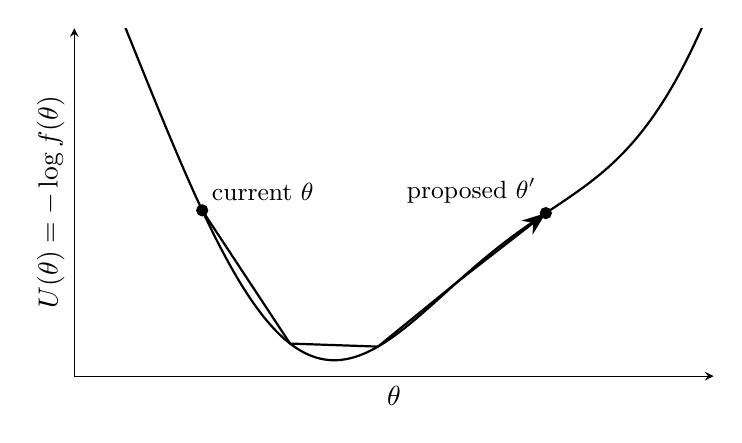
\begin{tikzpicture}
\begin{axis}[
    width=0.80\textwidth,
    height=6cm,
    xlabel={$\theta$},
    ylabel={$U(\theta) = -\log f(\theta)$},
    xmin=-4, xmax=4,
    ymin=-0.2, ymax=8.5,
    axis lines=left,
    ticks=none,
    domain=-4:4,
    samples=200,
]
% A smooth "potential energy" curve (illustrative)
\addplot[thick] {0.6*(x^2) + 1.2*sin(deg(1.2*x)) + 0.8};

% Mark a current state and a proposed far state along a "trajectory"
\addplot[only marks, mark=*, mark size=2pt] coordinates {(-2.4, {0.6*(2.4^2) + 1.2*sin(deg(1.2*(-2.4))) + 0.8})};
\addplot[only marks, mark=*, mark size=2pt] coordinates {( 1.9, {0.6*(1.9^2) + 1.2*sin(deg(1.2*( 1.9))) + 0.8})};

\node[anchor=south west] at (axis cs:-2.4, {0.6*(2.4^2) + 1.2*sin(deg(1.2*(-2.4))) + 0.8})
{\small current $\theta$};

\node[anchor=south east] at (axis cs:1.9, {0.6*(1.9^2) + 1.2*sin(deg(1.2*(1.9))) + 0.8})
{\small proposed $\theta'$};

% A stylized guided path (not exact dynamics; pedagogical)
\addplot[
  thick,
  -{Stealth[length=3mm]},
] coordinates {
  (-2.4, {0.6*(2.4^2) + 1.2*sin(deg(1.2*(-2.4))) + 0.8})
  (-1.3, {0.6*(1.3^2) + 1.2*sin(deg(1.2*(-1.3))) + 0.8})
  (-0.2, {0.6*(0.2^2) + 1.2*sin(deg(1.2*(-0.2))) + 0.8})
  ( 0.8, {0.6*(0.8^2) + 1.2*sin(deg(1.2*( 0.8))) + 0.8})
  ( 1.9, {0.6*(1.9^2) + 1.2*sin(deg(1.2*( 1.9))) + 0.8})
};

\end{axis}
\end{tikzpicture}
\caption{Illustration of the HMC intuition in one dimension. The posterior density
$f(\theta)$ is converted into a potential energy $U(\theta)=-\log f(\theta)$.
Hamiltonian dynamics use gradients of $U(\theta)$ (equivalently, of $\log f(\theta)$)
to propose long, coherent moves from a current value $\theta$ to a distant candidate
$\theta'$, avoiding the diffusive behavior of random-walk proposals.}
\label{fig:hmc_potential_intuition}
\end{figure}

\subsection{Hamiltonian dynamics and the proposal mechanism}

HMC generates proposals by simulating \emph{Hamiltonian dynamics},
defined by the system of differential equations
\begin{align}
\frac{d\boldsymbol{\theta}}{dt}
&=
\phantom{-}\frac{\partial H}{\partial \boldsymbol{p}}
=
\mathbf{M}^{-1}\boldsymbol{p},
\\[4pt]
\frac{d\boldsymbol{p}}{dt}
&=
-\frac{\partial H}{\partial \boldsymbol{\theta}}
=
-\nabla_{\boldsymbol{\theta}} U(\boldsymbol{\theta})
=
\nabla_{\boldsymbol{\theta}} \log f(\boldsymbol{\theta}).
\end{align}

These equations show explicitly how the \emph{gradient of the log posterior}
is exploited. The dynamics push the parameter vector $\boldsymbol{\theta}$
toward regions of high posterior density while preserving the total
energy $H$.

Two fundamental properties of Hamiltonian dynamics are essential for MCMC:
\begin{itemize}
  \item they are \emph{volume preserving}, meaning that the transformation
        has unit Jacobian;
  \item they are \emph{time reversible}.
\end{itemize}
These properties ensure that the resulting proposal can be embedded
within a Metropolis--Hastings accept--reject step.

\subsection{The leapfrog integrator}

In practice, the differential equations above cannot be solved exactly.
HMC therefore relies on a numerical scheme known as the
\emph{leapfrog integrator}, which approximates the dynamics using a step
size $\varepsilon$.

Given a current state $(\boldsymbol{\theta}, \boldsymbol{p})$, one leapfrog
step consists of:
\begin{align*}
\boldsymbol{p}\!\left(t + \tfrac{\varepsilon}{2}\right)
&=
\boldsymbol{p}(t)
+
\tfrac{\varepsilon}{2}\,
\nabla_{\boldsymbol{\theta}} \log f(\boldsymbol{\theta}(t)),
\\
\boldsymbol{\theta}(t + \varepsilon)
&=
\boldsymbol{\theta}(t)
+
\varepsilon\, \mathbf{M}^{-1}
\boldsymbol{p}\!\left(t + \tfrac{\varepsilon}{2}\right),
\\
\boldsymbol{p}(t + \varepsilon)
&=
\boldsymbol{p}\!\left(t + \tfrac{\varepsilon}{2}\right)
+
\tfrac{\varepsilon}{2}\,
\nabla_{\boldsymbol{\theta}} \log f(\boldsymbol{\theta}(t + \varepsilon)).
\end{align*}

The leapfrog scheme is carefully designed to preserve reversibility and
volume, and to approximately conserve the Hamiltonian. As a result,
large moves in parameter space can be proposed with high acceptance
probability.


\subsection{Metropolis correction}

After $L$ leapfrog steps, the algorithm produces a proposal
$(\boldsymbol{\theta}', \boldsymbol{p}')$. Because numerical integration
introduces small errors, the Hamiltonian is not exactly preserved. The
proposal is therefore accepted with probability
\begin{equation}
\alpha
=
\min\!\left(
1,
\exp\!\left[
- H(\boldsymbol{\theta}', \boldsymbol{p}')
+ H(\boldsymbol{\theta}, \boldsymbol{p})
\right]
\right).
\end{equation}

If the proposal is accepted, the new state of the chain is
$\boldsymbol{\theta}'$; otherwise, the chain remains at
$\boldsymbol{\theta}$. This correction step guarantees that the Markov
chain has the desired stationary distribution.

\begin{figure}[ht]
\centering
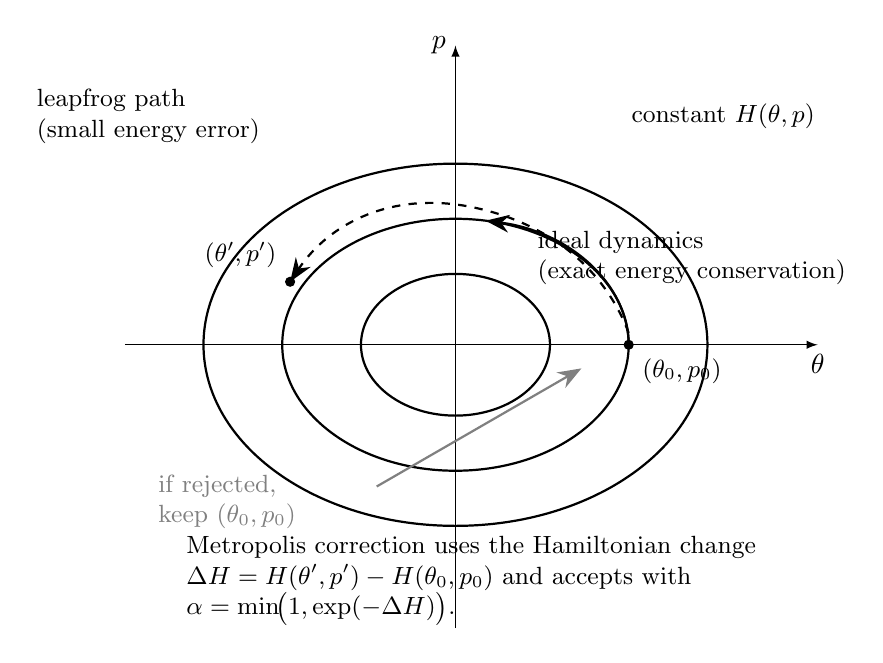
\begin{tikzpicture}[
  arr/.style={-{Stealth[length=3mm]}, thick},
  pt/.style={circle, fill, inner sep=1.3pt},
  lab/.style={font=\small}
]

% Axes
\draw[-latex] (-4.2,0) -- (4.6,0) node[below] {$\theta$};
\draw[-latex] (0,-3.6) -- (0,3.8) node[left] {$p$};

% "Energy" level sets (ellipses): H(theta,p)=U(theta)+K(p)
% Interpretable as constant-energy orbits in phase space.
\foreach \a/\b in {1.2/0.9, 2.2/1.6, 3.2/2.3} {
  \draw[thick] (0,0) ellipse (\a cm and \b cm);
}

\node[lab] at (3.4,2.9) {constant $H(\theta,p)$};

% Ideal continuous Hamiltonian trajectory: stays on one ellipse
\draw[arr] (2.2,0) arc[start angle=0, end angle=80, x radius=2.2, y radius=1.6];
\node[lab, align=left] at (3.0,1.1)
{ideal dynamics\\(exact energy conservation)};

% Leapfrog numerical trajectory: slightly off the ellipse (energy error)
% Draw a nearby "numerical" curve with a small radial drift
\draw[arr, dashed] (2.2,0.15)
  .. controls (1.9,0.95) and (1.2,1.55) .. (0.2,1.75)
  .. controls (-0.8,1.95) and (-1.6,1.55) .. (-2.1,0.8);

\node[lab, align=left] at (-3.9,2.9)
{leapfrog path\\(small energy error)};

% Mark start and end points
\node[pt, label={[lab]below right:{$(\theta_0,p_0)$}}] (s) at (2.2,0) {};
\node[pt, label={[lab]above left:{$(\theta',p')$}}] (e) at (-2.1,0.8) {};

% Explain acceptance rule
\node[lab, align=left] at (0.2,-3.0)
{Metropolis correction uses the Hamiltonian change\\
$\Delta H = H(\theta',p') - H(\theta_0,p_0)$ and accepts with\\
$\alpha = \min\!\bigl(1, \exp(-\Delta H)\bigr)$.};

% Add a small "rejection" arrow to show return to start (conceptual)
\draw[arr, gray] (-1.0,-1.8) -- (1.6,-0.3);
\node[lab, gray, align=left] at (-2.9,-2.0)
{if rejected,\\keep $(\theta_0,p_0)$};

\end{tikzpicture}
\caption{Phase-space view of HMC in one dimension. By introducing a momentum
variable $p$, the sampler simulates (approximate) Hamiltonian dynamics in the
augmented space $(\theta,p)$. Exact dynamics would conserve the Hamiltonian
$H(\theta,p)=U(\theta)+K(p)$ and move along a constant-energy contour. The leapfrog
integrator is reversible and volume preserving but introduces a small numerical
energy error $\Delta H$. The Metropolis accept/reject step corrects for this error,
accepting the proposed state with probability $\alpha=\min(1,e^{-\Delta H})$.
As the step size decreases, $\Delta H$ tends to be smaller and acceptance tends
to increase.}
\label{fig:hmc_phase_space}
\end{figure}

\subsection{Automatic tuning with NUTS}

Choosing the number of leapfrog steps $L$ is difficult in practice.
PyMC therefore uses the \emph{No-U-Turn Sampler} (NUTS), which dynamically
extends the Hamiltonian trajectory forward and backward in time until
it detects that the path is starting to reverse direction.

NUTS eliminates the need for manual tuning of $L$ while preserving the
same theoretical guarantees as HMC. From the user’s perspective, only a
target acceptance rate must be specified, and the sampler adapts
internally to the geometry of the posterior distribution.

\begin{figure}[ht]
\centering
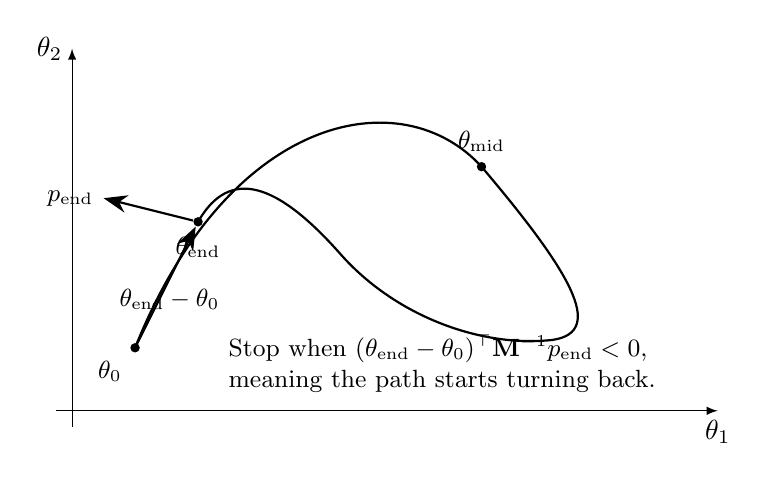
\begin{tikzpicture}[
  arr/.style={-{Stealth[length=3mm]}, thick},
  pt/.style={circle, fill, inner sep=1.2pt},
  lab/.style={font=\small}
]
% Axes
\draw[-latex] (-0.2,0) -- (8.2,0) node[below] {$\theta_1$};
\draw[-latex] (0,-0.2) -- (0,4.6) node[left] {$\theta_2$};

% A stylized trajectory
\draw[thick] (0.8,0.8)
  .. controls (2.0,3.8) and (4.2,4.2) .. (5.2,3.1)
  .. controls (6.3,1.8) and (6.8,1.0) .. (6.1,0.9)
  .. controls (5.2,0.8) and (4.1,1.2) .. (3.4,2.0)
  .. controls (2.6,2.9) and (2.0,3.1) .. (1.6,2.4);

% Mark points: start, intermediate, end
\node[pt, label={[lab]below left:{$\boldsymbol{\theta}_0$}}] (t0) at (0.8,0.8) {};
\node[pt, label={[lab]above:{$\boldsymbol{\theta}_{\text{mid}}$}}] (tm) at (5.2,3.1) {};
\node[pt, label={[lab]below:{$\boldsymbol{\theta}_{\text{end}}$}}] (te) at (1.6,2.4) {};

% A chord vector (start to end)
\draw[arr] (t0) -- node[lab, below, pos=0.55] {$\boldsymbol{\theta}_{\text{end}}-\boldsymbol{\theta}_0$} (te);

% A momentum direction at the end (stylized)
\draw[arr] (te) -- ++(-1.2,0.3) node[lab, left] {$\boldsymbol{p}_{\text{end}}$};

% U-turn condition illustration (dot product)
\node[lab, align=left] at (4.7,0.6)
{$\text{Stop when }(\boldsymbol{\theta}_{\text{end}}-\boldsymbol{\theta}_0)^\top \mathbf{M}^{-1}\boldsymbol{p}_{\text{end}} < 0,$\\
meaning the path starts turning back.};

\end{tikzpicture}
\caption{Geometric intuition for the NUTS stopping rule. NUTS grows a Hamiltonian
trajectory and stops when the direction of travel (represented by the momentum)
starts pointing back toward earlier states, indicating a ``U-turn.'' This avoids
wasting computation on trajectories that retrace their steps, and removes the need
to manually choose the number of leapfrog steps.}
\label{fig:nuts_uturn}
\end{figure}
\subsection{Implications for Bayesian estimation}

Compared to standard Metropolis--Hastings algorithms, HMC and NUTS:
\begin{itemize}
  \item exploit gradients of the log posterior to guide proposals,
  \item generate long-distance moves with high acceptance rates,
  \item handle strong posterior correlations efficiently,
  \item scale well to high-dimensional parameter spaces.
\end{itemize}

These properties explain why PyMC can reliably estimate complex Bayesian
choice models, latent-variable models, and mixture models that would be
computationally prohibitive with simpler MCMC methods.


\paragraph{Bibliographic pointers.}

The Metropolis--Hastings accept--reject framework dates to \citeasnoun{Metropolis1953} and \citeasnoun{Hastings1970}. The
original ``hybrid/Hamiltonian'' Monte Carlo construction in statistics
and lattice field theory is due to \citeasnoun{Duane1987}. A
widely cited modern reference that derives HMC from Hamiltonian
mechanics, explains the role of momentum variables and the mass
matrix, and connects energy conservation to high acceptance rates is
Neal’s handbook chapter (\cite{Neal2011}). Practical and geometric
intuition about HMC diagnostics (energy error, divergences, tuning,
mass-matrix adaptation) is emphasized by
\citeasnoun{Betancourt2017}. The No-U-Turn Sampler (NUTS), which
removes the need to hand-tune the path length, is introduced by
\citeasnoun{HoffmanGelman2014}. The leapfrog
(Störmer--Verlet) integrator used in HMC is a standard symplectic,
reversible, volume-preserving method; a canonical reference on
symplectic integrators and geometric numerical integration is \citeasnoun{HairerLubichWanner2006}. For extensions that
exploit local curvature via Riemannian geometry (conceptually related
to mass-matrix design), see \citeasnoun{GirolamiCalderhead2011}.

\section{How PyMC implements implicit integration over random parameters.}
\label{sec:pymc_random}
The key reason why Bayesian estimation in \textsc{Biogeme}, via PyMC, does not require explicit Monte--Carlo integration lies in the way the probabilistic model is constructed and sampled. In PyMC, all unknown quantities are represented as random variables within a single joint probabilistic model. This includes both the structural parameters (such as mean taste coefficients) and the random parameters associated with individual heterogeneity. In other words, the random coefficients that would traditionally be integrated out in a mixture of logit likelihood are explicitly introduced as latent variables in the model.

Formally, let $\boldsymbol{\beta}$ denote the population-level parameters and let
$\boldsymbol{\eta}_n$ denote the individual-specific random coefficients for individual $n$.
Instead of defining a marginal likelihood of the form
\[
p(y_n \mid \boldsymbol{\beta})
=
\int p(y_n \mid \boldsymbol{\eta}_n)\,
p(\boldsymbol{\eta}_n \mid \boldsymbol{\beta})\,
d\boldsymbol{\eta}_n,
\]
PyMC defines the joint posterior
\[
p(\boldsymbol{\beta}, \boldsymbol{\eta}_{1:N} \mid \mathcal{D})
\propto
\left[
\prod_{n=1}^N
p(y_n \mid \boldsymbol{\eta}_n)
\, p(\boldsymbol{\eta}_n \mid \boldsymbol{\beta})
\right]
p(\boldsymbol{\beta}),
\]
where $\mathcal{D}$ denotes the observed choices. The individual-level random
coefficients $\boldsymbol{\eta}_n$ are treated exactly like any other unknown
parameter and are sampled jointly with $\boldsymbol{\beta}$ by the MCMC
algorithm.

During sampling, PyMC repeatedly generates draws
\[
\bigl(\boldsymbol{\beta}^{(s)}, \boldsymbol{\eta}_{1:N}^{(s)}\bigr),
\qquad s = 1, \dots, S,
\]
from this joint posterior distribution. Conditional on a given draw
$\boldsymbol{\eta}_n^{(s)}$, the likelihood contribution of observation $n$
is simply the kernel of the elementary discrete choice model, typically a
logit probability. The role that numerical integration plays in classical
maximum likelihood estimation is thus replaced by averaging over posterior
draws:
\[
p(y_n \mid \boldsymbol{\beta})
\approx
\frac{1}{S} \sum_{s=1}^S
p\!\left(y_n \mid \boldsymbol{\eta}_n^{(s)}\right),
\]
where the averaging is performed implicitly by the MCMC procedure itself.

From the user's perspective, this has an important practical implication.
When specifying a mixture model in \textsc{Biogeme}, one does not write the
integrated (mixed) likelihood. Instead, one provides only the conditional
log-likelihood of the elementary model, given a realization of the random
coefficients. PyMC handles the sampling of the latent random parameters and,
through Monte--Carlo averaging over the posterior draws, automatically
approximates the required integrals. This approach is both theoretically
exact in the limit of an infinite number of draws and numerically stable,
as it avoids introducing simulation noise directly into the likelihood
evaluation.
\clearpage
\bibliographystyle{dcudoi}
\bibliography{transpor}

\end{document}


